% Possible use http://www.latextemplates.com/template/the-legrand-orange-book as template? See https://www.overleaf.com/9174958nyjxxdxbchks#/33024595/

\documentclass[11pt,letterpaper,fleqn]{memoir} % Default font size and left-justified equations


\usepackage[top=3cm,bottom=3cm,left=3cm,right=3cm,headsep=10pt,letterpaper]{geometry} % Page margins

% Theorem definitions using amsthm

\usepackage{amsthm}
\usepackage{amsmath}
\usepackage{amssymb}

% Remove line spaces between items of enumerate and itemize
\usepackage{enumitem}
\setlist{noitemsep}


% Adds double bracket symbols
\usepackage{stmaryrd}

% Latex symbol guide at http://mirrors.ibiblio.org/CTAN/info/symbols/comprehensive/symbols-letter.pdf

% LOGIC symbols
% -------------

% Allows to create negation symbols
\usepackage{MnSymbol}

\DeclareMathOperator{\truth}{truth}
\DeclareMathOperator{\poss}{possibilities}
\DeclareMathOperator{\result}{result}

\def\TRUE{\textsc{true}}
\def\FALSE{\textsc{false}}

\def\SUCCESS{\textsc{success}}
\def\FAILURE{\textsc{failure}}
\def\UNDEF{\textsc{undefined}}


% Symbols for tautology and contradiction
\def\tautology{\top}
\def\contradiction{\bot}

% Symbols for "compatibility" and "incompatibility"
\def\comp{\doublefrown}
\def\ncomp{\ndoublefrown}

% Symbols for "narrower" and "wider"
\def\narrower{\subseteq}
\def\nnarrower{\nsubseteq}
\def\broader{\supseteq}
\def\nbroader{\nsupseteq}


% Symbol for "independent" and "correlated"
\def\indep{\upmodels}
\def\nindep{\nupmodels}

% Aliases for logical operations
\def\AND{\wedge}
\def\bigAND{\bigwedge}
\def\OR{\vee}
\def\bigOR{\bigvee}
\def\NOT{\neg}


% Formatting for statements
\newcommand{\stmt}[1][s] {\mathsf{#1}}
% Formatting for experimental tests
\newcommand{\expt}[1][e] {\mathsf{#1}}
% Formatting for observations
\newcommand{\obs}[1] {\mathsf{#1}}
% Formatting for observation definition
\newcommand{\obsdef}[2] {\llparenthesis #1, #2 \rrparenthesis}

% Formatting for experimental domain
\newcommand{\edomain}[1][D] {\mathcal{#1}}

% Formatting for theoretical domain
\newcommand{\tdomain}[1][D] {\bar{\mathcal{#1}}}


% Formatting for sentence statements
\newcommand{\statement}[1] {\emph{``#1"}}


\usepackage{xcolor} % Required for specifying colors by name
\definecolor{sectionNumbers}{RGB}{44, 103, 0}


\renewcommand\thesubsection{\thesection.\Alph{subsection}}
\renewcommand{\theequation}{\thechapter.\arabic{equation}}

\newtheorem{assump}{Assumption}
\renewcommand*{\theassump}{\Roman{assump}}

\newtheorem{defn}[equation]{Definition}
\newtheorem{prop}[equation]{Proposition}

%\theoremstyle{definition}

\newenvironment{rationale}{\emph{Rationale}.}{\qed}
\newenvironment{justification}{\emph{Justification}.}{\qed}
\renewenvironment{proof}{\emph{Proof}.}{\qed}

% Style for math section
\RequirePackage[framemethod=default]{mdframed} % Required for creating the theorem, definition, exercise and corollary boxes
\newmdenv[skipabove=7pt,
skipbelow=7pt,
rightline=false,
leftline=true,
topline=false,
bottomline=false,
linecolor=sectionNumbers,
backgroundcolor=black!2,
innerleftmargin=5pt,
innerrightmargin=5pt,
innertopmargin=5pt,
leftmargin=0cm,
rightmargin=0cm,
linewidth=4pt,
innerbottommargin=5pt]{mathSection}


%----------------------------------------------------------------------------------------
%	SECTION NUMBERING IN THE MARGIN
%----------------------------------------------------------------------------------------

\makeatletter
\renewcommand{\@seccntformat}[1]{\llap{\textcolor{sectionNumbers}{\csname the#1\endcsname}\hspace{1em}}}                    
\renewcommand{\section}{\@startsection{section}{1}{\z@}
	{-4ex \@plus -1ex \@minus -.4ex}
	{1ex \@plus.2ex }
	{\normalfont\large\sffamily\bfseries}}
\renewcommand{\subsection}{\@startsection {subsection}{2}{\z@}
	{-3ex \@plus -0.1ex \@minus -.4ex}
	{0.5ex \@plus.2ex }
	{\normalfont\sffamily\bfseries}}
\renewcommand{\subsubsection}{\@startsection {subsubsection}{3}{\z@}
	{-2ex \@plus -0.1ex \@minus -.2ex}
	{.2ex \@plus.2ex }
	{\normalfont\small\sffamily\bfseries}}                        
\renewcommand\paragraph{\@startsection{paragraph}{4}{\z@}
	{-2ex \@plus-.2ex \@minus .2ex}
	{.1ex}
	{\normalfont\small\sffamily\bfseries}} % Loads the book formatting
\usepackage{tikz}

\newif\ifdraft

\drafttrue
%\draftfalse

\newcommand{\bookversion}{1.1}
\newcommand{\bookdate}{March 8, 2021}

% Adding ability to include pdfs (used to import book cover)
\usepackage{pdfpages}

% Adding pdf index and links within the document
% Custom formatting to remove default red boxes
\usepackage{hyperref}
\hypersetup{
	colorlinks=true,
    urlcolor=blue,
    linkcolor=blue
}
\urlstyle{same}
% ---------------------------

\DeclareMathOperator{\tr}{tr}

\usetikzlibrary{positioning,calc,arrows,arrows.meta, shapes}


\begin{document}
	
% Set theory (expected) \in, \subset, injective/surjective, cartesian product

% Closure of a set under an operation

% Need examples of topology and sigma algebra

% Note that sigma algebra are also closed under intersections

% TODO: language change. Possibilities are experimentally DEFINED cases. Experimentally distinguishable cases give Hausdorff.

\frontmatter
\thispagestyle{empty} % Suppress headers and footers on the title page

\includepdf{BookCover.pdf}
\newpage
\thispagestyle{empty}
~
\newpage

~
\thispagestyle{empty}

\vspace{20pt}

{\large \noindent Gabriele Carcassi, Christine A. Aidala }

\vspace{60pt}

{\Huge \noindent \textbf{Assumptions of physics}}

\vspace{30pt}

\ifdraft {\large \noindent Working DRAFT for Ver \bookversion  ~- \today}
\else {\large \noindent Ver \bookversion  ~- \bookdate}
\fi

\vfill

%\chapter*{Assumptions of physics}

\ifdraft 
\noindent \textbf{This book is a work in progress}. This draft is a development copy built on \today. It is provided as-is for the purpose of early review and feedback. You can get the latest draft from \url{https://assumptionsofphysics.org/book}. 
\else
\noindent This edition was finalized on \bookdate. For changes since then, you can get the latest draft from \url{https://assumptionsofphysics.org/book}.
\fi

\newpage
~\vfill
\thispagestyle{empty}

% Copyright notice
\noindent Copyright \copyright\ 2018-21 Gabriele Carcassi, Christine A. Aidala

\vspace{12pt}

% Link to website
\noindent \textsc{assumptionsofphysics.org/book}

\vspace{12pt}

% License
\noindent Licensed under the Attribution-NonCommercial-ShareAlike 4.0 International (CC BY-NC-SA 4.0) (the ``License"). You may not use this file except in compliance with the License. You may obtain a copy of the License at https://creativecommons.org/licenses/by-nc-sa/4.0/. This work is distributed under the License ``as is'', without warranties or conditions of any kind, either express or implied.

\chapter{Preface}

This work is part of a larger project, Assumptions of Physics (\url{https://assumptionsofphysics.org}), that aims to identify a handful of physical principles from which the basic laws can be rigorously derived. The aim is to give physics (and science more in general) a renewed foundation that is mathematically precise, physically meaningful and philosophically consistent. This work contains only the parts of the project that are considered to be mature enough to meet that high standard, and therefore will be expanded as progress is being made. We give here a brief overview of the project, which can be useful to better understand the context of this work.

\subsection{Overall goals of Assumptions of Physics}

What do the basic laws of physics describe? Why is the state of a classical particle identified by position and momentum (i.e.~a point on a symplectic manifold) while the state of a quantum system is identified by a wave function (i.e.~a vector in a Hilbert space)? What assumptions are unique to each theory? What are, instead, the basic requirements that all physical theories must satisfy? Could we have had different laws? A lack of clear answers to these questions is, we believe, the biggest obstacle in the foundations of physics and prevents the resolution of outstanding problems in the field. \textbf{Our approach is to find a minimal set of physical assumptions that are necessary and sufficient to derive the different theories within a unified framework.} If we are able to do so, then we are guaranteed that all that the laws of physics say is encoded in those assumptions and we are able to answer those questions.

We found this approach to be very fruitful. It provides new insights into physics as a whole, the role of mathematics in physical theories and a gives a more solid conceptual foundation to both. It becomes clear why some mathematical structures are pervasive in science and what exactly they are meant to represent, while others will never play a role. The downside is that we have to touch many subjects in math (logic, topological spaces, measure theory, group theory, vector spaces, differential geometry, symplectic geometry, statistics, probability theory, ...), physics (Hamiltonian mechanics, Lagrangian mechanics, thermodynamics, quantum mechanics, electromagnetism, ...) and science in general (computer science theory, information theory, system theory, ...). In other words, \textbf{the only way to properly achieve the goal is to rebuild everything from the ground up:} formal rigor, physical significance and conceptual integrity are not something that can be added at the end, but they must be present from the beginning.

The main takeaway for us is that the foundations of science are one: no real progress can be made on the foundations of one subject without making progress on the foundations of others. \textbf{What is needed is a general theory of experimental science: a theory that studies physical theories.} This provides a standard framework that defines basic concepts and requirements (e.g.~experimental verifiability, granularity of descriptions, processes and states) that serve as a common basis for all theories. Each theory, then, is recovered by studying how these common objects become specialized under different assumptions. This book aims to build over time, piece by piece, this framework.

While the topic is necessarily inter-disciplinary, \textbf{this is still first and foremost a scientific book}. The material should be accessible to the mathematician and philosopher, but understand that it needs to resonate first and foremost with the experimental physicist and the engineer. The mathematical definitions and derivations are there to make the science precise, but they are not the main focus. In fact, the book is designed so that the mathematical definitions and proofs, highlighted with a green side bar, can be skipped altogether without loss of the big picture and the important details. Along the same line, the foundational discussions are there to articulate more precisely what it means to do science, so they will not indulge in other questions which may be of interest to the philosopher but not to the scientist.

\subsection{A living work}

For the project to be successful, we need to depart from some of the norms of academic research and academic publishing. For example, one typically develops his research program as a series of articles published in a peer reviewed journal that caters to a specific community. These articles are then typically collected as is or merged into a book. This does not work for this project. As journals are specialized into sometimes very narrow fields, this would create a set of disjoint articles that cater to different audiences, with no guarantee that they can fit into a unified vision. For us, the overall picture, if and how the different perspectives combine, is the most important feature. \textbf{In this sense, the book comes first and the articles are derivative works.} We need to pool expertise and ideas from a wide range of disciplines and make sure that the result makes sense from all angles.

As the goal is broad, the framework needs to evolve as new issues are solved and old ones are better understood. If one part changes, we have to make sure that everything is updated to keep conceptual consistency. \textbf{This book, therefore, is an ongoing project.} It will continue to grow organically, adding and revising chapters. As is standard practice in open source/free software communities, we need to ``release early, release often'' to gather feedback. Each new version supersedes all prior ones and will be superseded by future ones. There is therefore no ``definitive version'' in the near future as we don't expect to ``solve all of physics'' in the near future. However, the framework will tend to converge as different parts become more settled.

The upshot is that one only needs to read the latest version of this work to be current. That is, one does not need to read a scattered set of papers, which require previous knowledge of a field, and follow how the ideas have changed. Just get the latest copy of the book, and if you do find areas you can help us expand or improve, let us know!

\subsection{A new standard for scientific rigor}

The standard of rigor mathematicians have developed for their field is not sufficient for the purpose of this project. Mathematics only deals with formal systems, whose starting points are a set of definitions and rules that are taken as is. At that point, correctness of the premise cannot be established, only self-consistency. Therefore mathematics fails to deal with the most delicate and interesting parts of the foundations of physics: the physical assumptions and how they are encoded into the formal framework. We therefore need rules and standards for rigorously handling the informal parts of the framework and, since there are no guidelines for this, we set our own standard.

We call an \textbf{axiom} a proposition that brings new objects or new properties of established objects within the formal framework. A \textbf{definition}, instead, is a proposition that further characterizes objects and properties already present in the formalism. \textbf{An axiom or a definition is well posed only when it is clear what the objects represent physically and what aspects are captured mathematically.} Therefore each axiom and definition is composed of two parts. The first characterizes the objects and properties within the informal system, tells us what they represent physically. The second part, typically preceded by ``Formally'', characterizes the part that is captured by the formal system. Axioms and definitions are followed by a \textbf{justification} when it is necessary to explain why the elements in the informal system must be mapped into the formal system in the way proposed. Some definitions are purely formal and as such do not require justifications. As this argument spans both the formal and informal systems, this cannot be a mathematical proof in the modern sense. In particular, the justification for an axiom must argue why those objects must exist.

\textbf{The above standard makes sure we have a perfect identification between formal and informal objects.} All mathematical symbols correspond to physical objects and all the relevant physical concepts are captured by the math. All subsequent propositions and proofs, then, can be carried out in the formal system, where it is easier to check for consistency and correctness. However, all the proofs can, if need be, be translated into the informal language and given physical meaning.

\section{Project overview}

Here we present a summary of the whole project and the status of each part as the layout will map to the structure of this work. As of now, the book only covers the first part of the project (experimental verifiability) as it is the only one fully developed to the required level of rigor. However, this has to be understood in the greater context of the work. There would be no point in making the beginning rigorous if we did not expect to be able to use it as a foundation for the actual physical theories.

\subsection{General theory}

The general mathematical theory of experimental science, or simply general theory, lays down the basic axioms and definitions that are required for any physical theory. \textbf{It provides a ``theory of scientific theories'' that allows us to define and study the set of all well-formed scientific theories.} The core tenet is the principle of scientific objectivity: ``Science is universal, non-contradictory and evidence based.'' This serves to define the subject and the basic formal requirements of a scientific theory. We divide the general theory into three main parts.

\begin{description}
	\item[Experimental verifiability.] This part defines a scientific theory as a set of statements. It provides the basic axioms which simply characterize the rules of logic as applied to experimentally verifiable statements. Mathematically, these requirements are captured by topologies and $\sigma$-algebras over the space of the possible cases that can be identified experimentally. This part is very well developed both conceptually and mathematically, and it is the only part currently included in this book. 
	
	\item[Informational granularity.] This part adds the ability to compare the level of description of different statements. Mathematically, this imposes a preorder on the algebra of statements which is intended to provide a common foundation to geometry, measure theory, probability theory and information theory. All those structures, in fact, provide ways to compare the size of sets of possible cases and the description provided in terms of those sets. This part is fairly developed conceptually but not yet well developed mathematically.
	
	\item[States and processes.] This part defines the basic physical notions of processes, systems and states. It serves to bring to light a series of hidden assumptions that are needed, both physically and mathematically, to be able to talk about independent systems. These will lead to notions of entropy, state spaces and the geometrical structures that accompany them. This part is still being developed conceptually, though the progress is encouraging.
\end{description}

\subsection{Physical theories}

Once the general theory is laid out, we can understand how different assumptions lead to the different physical theories. Assumptions essentially puts constraints on the logical structures defined above, and those constraints lead to more specialized mathematical structures, the ones we are already familiar with. This part is already fairly developed both conceptually and mathematically. However, it is developed in the opposite direction, by reverse engineering the current theories. Therefore it requires the reconstruction of fairly broad parts of mathematics to be brought to the level of rigor we envision and be included in this book.

\begin{description}
	\item[Determinism and reversibility:] ``The system under study undergoes deterministic and reversible evolution." Mathematically, the physical properties of the system determine which category, in the mathematical sense, is used to describe the state space and deterministic, and reversible evolution will be an isomorphism in the category (i.e.~a bijective map that preserves the physical properties of the system). Therefore the law of evolution is not just a bijective map, but is also a linear transformation, a differentiable map or an isometry depending on the context.
	
	\item[Infinitesimal reducibility:] ``Knowing the state of the whole system is equivalent to knowing the state of all its infinitesimal parts." For example, we can study the motion of a ball, but we can also mark a spot in red and study the motion of the mark. Knowing the evolution of the whole ball means knowing the evolution of any arbitrary spot and vice-versa. Mathematically, the state of the whole will be a distribution over the state space of the parts. It will need to be a distribution whose value is invariant under coordinate transformations. The state space of the infinitesimal parts, then, comes equipped with an invariant two-form upon which we can define such a distribution. The state space is therefore a symplectic manifold and the deteministic and reversible evolution is a symplectomorphism. That is, the infinitesimal parts follow classical Hamiltonian mechanics. Proper handling of the time variable will give us a relativistic version of the framework without extra assumptions.
	 
	\item[Irreducibility:] ``Knowing the state of the whole system tells us nothing about its infinitesimal parts." For example, we can study the state of an electron by scattering photons off of it. But whenever a photon interacts with the electron, it interacts with the whole electron. There is no way to mark a part of an electron and study it independently from the rest. Mathematically, the state of the electron will be a distribution that evolves deterministically where the motion of each infinitesimal part evolves randomly. A complex vector space will be the appropriate tool to keep track of the internal chaotic motion leading to quantum mechanics.
	
	\item[Kinematic equivalence:] ``Knowing the state of the system is equivalent to knowing its trajectory and vice-versa." This means that we will have to be able to transfer a distribution over state variables (i.e.~position and momentum) into a distribution over kinematic variables (i.e.~position and velocity). Mathematically, the symplectic two-form will induce a symmetric tensor over the tangent space for position. This will give us a metric and will also allow us to reformulate the laws of motion according to Lagrangian mechanics. Because the transformation is linear, we are able to constrain the Hamiltonian to the one for massive particles under scalar and vector potential forces.
\end{description}

\section*{Current plan and status}

We usually proceed concurrently in two opposite directions. The bottom-up approach extends the precise formalization of the core framework. Currently, the goal is to work on informational granularity trying to characterize how the notion of finer descriptions puts a preorder on the algebra of statements that, in some conditions, leads to measure theory. The top-down approach takes physical theories and tries to extend the framework to accommodate them. Currently, the goal is to work on non-deterministic and non-reversible processes and understand how thermodynamics and statistical mechanics can be recovered.

\section*{Changelog}

\begin{description}
	\item 2018/06/22: Ver 0.1 - Consolidated first two chapters that lay the foundation for the general theory.
	\item 2019/02/22: Ver 0.2 - Consolidated third chaper on properties, quantities and ordering.
	\item 2019/07/07: Ver 0.3 - Reviewed first two chapters to clarify the idea of possible assignments and how contexts for function spaces are constructed.
	\item 2021/03/08: Ver 1.0 - Updated the first three chapters with minor changes: renamed tautology to certainty and contradiction to impossibility as they characterize better their role in the framework; made more formal justifications for the basic axioms and some of the basic definitions; causal relationships are now proved to be continuous instead of assumed to be continuous. Added Part II to include the results that are not yet fully formalized, to give a sense of the future scope of the work.
	\item : Ver ? - Added a few diagrams on the logic section.
\end{description}


\cleardoublepage % Forces the first chapter to start on an odd page so it's on the right

\tableofcontents* % Print the table of contents itself

\cleardoublepage % Forces the first chapter to start on an odd page so it's on the right

%\pagestyle{fancy} % Print headers again

\mainmatter

\part{Reverse Physics}

TODO: Write the intro to reverse physics.

For example

\chapter{Classical mechanics}

The standard view in physics is that classical mechanics is perfectly understood. It has three different but equivalent formulations, the oldest of which, Newtonian mechanics, is based on three laws. Classical mechanics is the theory of point particles that follow those laws. Unfortunately, this view is incorrect.

We will see that the three formulations are not equivalent, in the sense that there are physical systems that are Newtonian but not Hamiltonian and vice-versa. There are also a number of questions that have been left unanswered, such as the precise nature of the Hamiltonian or the Lagrangian, and what exactly the principle of stationary action represents physically. While shedding light on these issues, we will also find that classical mechanics already contains elements that are typically associated with other theories, such as quantum mechanics/field theories (uncertainty principle, anti-particles), thermodynamics/statistical mechanics (thermodynamic and information entropy conservation) or special relativity (energy as the time component of a four-vector). In other words, the common understanding of classical mechanics is quite shallow, and its foundations are, in fact, not separate from the ones of classical statistical mechanics or special relativity.

What reverse physics shows is that the central assumption underneath classical mechanics is that of \textbf{infinitesimal reducibility}: a classical system can be thought of as made of parts, which in turn are made of parts and so on; studying the whole system is equivalent to studying all its infinitesimal parts. This assumption, together with the assumption of \textbf{independence of degrees of freedom}, is what gives us the structure of classical phase space with conjugate variables. The additional assumption of \textbf{determinism and reversibility}, the fact that the description of the system at one time is enough to predict its future or reconstruct its past, leads us to Hamiltonian mechanics. On the other hand, assuming \textbf{kinematic equivalence}, the idea that trajectories in space are enough to reconstruct the state of the system and vice-versa, leads to Newtonian mechanics. The combination of all above assumptions, instead, leads to Lagrangian mechanics and, in particular, to massive particles under (scalar and vector) potential forces.

\section{Formulations of classical mechanics}

In this section we will briefly review the three main formulations of classical mechanics. Our task is not to present them in detail, but rather to provide a brief summary of the equations so that we can proceed with the comparison. In particular, given that different conventions are used across formulations, within the same formulation and among different contexts (e.g. relativity, symplectic geometry), we will want to make the notation homogeneous to allow easier comparisons.

\subsection{Newtonian mechanics}

For all formulations, the system is modeled as a collection of point particles, though we will mostly focus on the single particle case. For a Newtonian system, the state of the system at a particular time $t$ is described by the position $x^i$ and velocity $v^i$ of all its constituents. Each particle has its mass $m$, not necessarily constant in time, and, for each particle, we define kinetic momentum as $\Pi^i = m v^i$.\footnote{We will use the letter $t$ for the time variable, $x$ for position and $v$ for velocity, which is a very common notation in Newtonian mechanics. However, we will keep using the same letters in Lagrangian mechanics as well, instead of $q$ and $\dot{q}$, for consistency. Given that the distinction between kinetic and conjugate momentum is an important one, we will denote $\Pi$ the former and $p$ the latter. The Roman letters $i,j,k,...$ will be used to span the spatial components, while we will use the Greek letters $\alpha, \beta, \gamma, ...$ to span space-time components. Unlike some texts, $x^i$ do not represent Cartesian coordinates, and therefore they should be understood already as generalized coordinates.}

The evolution of our system is given by Newton's second law:\footnote{For derivatives, we will use the shorthand $d_t$ for $\frac{d}{dt}$ and $\partial_{x^i}$ for $\frac{\partial}{\partial x^i}$. }
\begin{equation}\label{rp-cm-NewtonsSecondLaw}
	F^i(x^j, v^k, t) = d_t \Pi^i.
\end{equation}
Mathematically, if the forces $F^i$ are Lipschitz continuous, then the solution $x^i(t)$ is unique. That is, given position and velocity at a given time, we can predict the position and velocity at future times. We will assume a Newtonian system has this property.

An important aspect of Newtonian mechanics is that the equations are not invariant under coordinate transformation. To distinguish between apparent forces (i.e. those dependent on the choice of frame) and the real ones, we assume the existence of inertial frames. In an inertial frame there are no apparent forces, and therefore a free system (i.e. no forces) with constant mass proceeds in a linear uniform motion, or stays still.\footnote{Recall that linear motion simply means that it describes a line in space, while uniform motion means that the speed is constant. Therefore we can have linear non-uniform notion (e.g. an object accelerated along the same direction) or a non-linear uniform motion (e.g. an object going around in a circle at constant speed).}

\subsection{Lagrangian mechanics}

The state for a Lagrangian system is also given by position $x^i$ and velocity $v^i$. The dynamics is specified by a single function $L(x^i, v^j, t)$ called the Lagrangian. For each spatial trajectory $x^i(t)$ we define the action as $\mathcal{A}[x^i(t)] = \int_{t_0}^{t_1} L(x^i(t), d_t x^i(t), t) dt$. The trajectory taken by the system is the one that makes the action stationary:
\begin{equation}
\delta \mathcal{A}[x^i(t)] = \delta \int_{t_0}^{t_1} L\left(x^i(t), d_t x^i(t), t\right) dt=0
\end{equation}
The evolution can equivalently be specified by the Euler-Lagrange equations:
\begin{equation}\label{rp-cm-EulerLagrange}
	\partial_{x^i}L=d_t \partial_{v^i} L.
\end{equation}

Note that not all Lagrangians lead to a unique solution. For example, $L=0$ will give the same action for all trajectories and therefore, strictly speaking, all trajectories are possible. The stationary action leads to a unique solution if and only if the Lagrangian is hyperregular, which means the Hessian matrix $\partial_{v^i}\partial_{v^j} L$ is invertible. Like in the Newtonian case, we will assume Lagrangian systems satisfy this property.

Unlike Newton's second law, both the Lagrangian and the Euler-Lagrange equations are invariant under coordinate transformations. This means that Lagrangian mechanics is particularly suited to study the symmetries of the system.

\subsection{Hamiltonian mechanics}

In Hamiltonian mechanics, the state of the system is given by position $q^i$ and conjugate momentum $p_i$. The dynamics is specified by a single function $H(q^i, p_j, t)$ called the Hamiltonian.\footnote{We use a different symbol for position in Hamiltonian mechanics because, while it is true that $q^i = x^i$, it is also true that $\partial_{q^i} \neq \partial_{x^i}$: the first derivative is taken at constant conjugate momentum while the second is taken at constant velocity. This creates absolute confusion when mixing and comparing Lagrangian and Hamiltonian concepts, which our notation avoids completely.} The evolution is given by Hamilton's equations:
\begin{equation}\label{rp-cm-HamiltonEq}
	\begin{aligned}
		d_t q^i = \partial_{p_i} H \\
		d_t p_i = - \partial_{q^i} H \\
	\end{aligned}
\end{equation}
We will again want these equations to yield a unique solution, which means the Hamiltonian must be at least differentiable, and the derivatives must at least be Lipschitz continuous.

Hamilton's equations are invariant as well. The Hamiltonian itself is a scalar function which is often considered (mistakenly as we'll see later) invariant. This formulation is the most suitable for statistical mechanics as volumes of phase space correctly count the number of possible configurations.

\section{Inequivalence of formulations}\label{rp-cm-inequivalenceOfFormulations}

It is often stated in physics books that all three formulations of classical mechanics are equivalent. We will look at this claim in detail, and conclude that this is not the case: there are systems that can be described by one formulation and not another. More precisely, the set of Lagrangian systems is exactly the intersection of Newtonian and Hamiltonian systems.

We will consider two formalisms equivalent if they can be applied to exactly the same systems. That is, Newtonian and Lagrangian mechanics are equivalent if any system that can be described using Newtonian mechanics can also be described by Lagrangian mechanics and vice-versa. In general, in physics great emphasis is put on systems that can indeed be studied by all three, leaving the impression that this is always doable.\footnote{If one asks the average physicist whether Newtonian and Hamiltonian mechanics are equivalent, the answer most of the time will be  enthusiastically positive. If one then asks for the Hamiltonian for a damped harmonic oscillator, the typical reaction is annoyance due to the nonsensical question (damped harmonic oscillators do not conserve energy), followed by a realization and partial retraction of the previous claim. The moral of the story is to never take these claims at face value.} However, just with a cursory glance, we realize that this can't possibly be the case.

The dynamics of a Newtonian system, in fact, is specified by three independently chosen functions of position and velocity, the forces applied to each degree of freedom. On the other hand, the dynamics of Lagrangian and Hamiltonian systems is specified by a single function of position and velocity/momentum, the Lagrangian/Hamiltonian. Intuitively, there are more choices in the dynamics for Newtonian systems than for Lagrangian and Hamiltonian.

Now, the reality is a bit trickier because the mathematical expression of the forces is not enough to fully characterize the physical system. We need to know in which frame we are, what coordinates are being used and the mass of the system, which is potentially a function of time. On the Lagrangian side, note that the Euler-Lagrange equations are homogeneous in $L$. This means that multiplying $L$ by a constant leads to the same solutions, meaning that the same system can be described by more than one Lagrangian. The converse is also true: if one system is half as massive and is subjected to a force half as intense, the resulting Lagrangian is also simply rescaled by a constant factor. Therefore the map between Lagrangians and Lagrangians system is not one-to-one: it is many-to-may. This is why we should never look simply at mathematical structures if we want to fully understand the physics they describe.

Regardless, our task is at the moment much simpler: we only need to show that there are Newtonian systems not expressible by Lagrangian or Hamiltonian mechanics. We can therefore limit ourselves to systems with a specific constant mass $m$ in an inertial frame. Every possible expression of the force is allowed and will lead to a unique expression of the acceleration $a^i=F^i(x^j, v^k, t)/m$ which means a unique set of possible trajectories for each expression of the force. Now, we can think of trying to write a Lagrangian for each of those systems. Assuming that this is possible, the acceleration $a^i=F^i[L]/m$ is going to be some functional of that Lagrangian, which, given the Euler-Lagrange equations \ref{rp-cm-EulerLagrange} must be continuous: for small variation of the Lagrangian we must have a small variation of the equations of motion and therefore of the acceleration. But a continuous surjective map from the space of a single function (i.e. the Lagrangian) to the space of multiple functions (i.e. those that specify the forces) does not exist, and therefore there must be at least one Netwonian system with constant mass expressed in an inertial frame that is not describable using Lagrangian mechanics. The same argument applies for Hamiltonian mechanics, since the dynamics in this case is also described by a single function in the same number of arguments. We therefore reach the following conclusion:
\begin{equation}
	\textrm{Not all Netwonian systems are Lagrangian and/or Hamiltonian.}
\end{equation}

We now want to understand whether all Lagrangian systems are Newtonian. Given what we discussed, we cannot expect to reconstruct the mass and force uniquely from the expression of the Lagrangian. We consider the mass and the frame fixed by the problem, together with the Lagrangian, and therefore we must only see whether we can indeed find a unique expression for the acceleration. From the Euler-Lagrange equations \ref{rp-cm-EulerLagrange} we can write
\begin{equation}
	\begin{aligned}
	\partial_{x^i}L&=d_t \partial_{v^i} L=\partial_{q^j} \partial_{v^i} L \, d_t q^j + \partial_{v^k} \partial_{v^i} L \, d_t v^k = \partial_{q^j} \partial_{v^i} L \, v^j + \partial_{v^k} \partial_{v^i} L \, a^k \\
	\partial_{v^k} &\partial_{v^i} L \, a^k = \partial_{x^i}L - \partial_{q^j} \partial_{v^i} L \, v^j .
	\end{aligned}
\end{equation}
To be able to write the acceleration explicitly, we must be able to invert the Hessian matrix $\partial_{v^k} \partial_{v^i} L$. As we noted before, this is exactly the condition for which the principle of stationary actios leads to a unique solution, and we can better understand why. If it is not invertible at a point, the determinant is zero and therefore one eigenvalue is zero. The corresponding eigenvector corresponds to a direction for which the equation tells us nothing, and therefore a variation of the acceleration in that direction will not change the action. This is why the invertibility of the Hessian is required in order to obtain unique solutions.

What we find, then, is that for any Lagrangian system, which we assume to have a unique solution, we can explicitly write the acceleration as a function of position, velocity and time. Therefore
\begin{equation}
	\textrm{All Lagrangian systems are Newtonian.}
\end{equation}

Now we turn our attention to Hamiltonian mechanics and, similarly, we ask whether we can express the acceleration as a function of position and velocity. We have
\begin{equation}
	\begin{aligned}
		a^i &= d_t v^i = d_t d_t q^i = d_t \partial_{p_i} H = \partial_{q^j} \partial_{p_i} H d_t q^j + \partial_{p_k} \partial_{p_i} H d_t p_k \\
		&= \partial_{q^j} \partial_{p_i} H \partial_{p_j} H - \partial_{p_k} \partial_{p_i} H \partial_{q^k} H.
	\end{aligned}
\end{equation}
This tells us that the acceleration is always an explicit function, but it is, in general, an explicit function of position and momentum, not of position and velocity. To change the expression, we need to be able to write the momentum as a function of position and velocity. Note that Hamilton's equations already give a way to express the velocity in terms of position and momentum, we just need that expression to be invertible, which means the Jacobian must be invertible. We must have:
\begin{equation}
	\left|\partial_{p_i} v^j\right| = \left|\partial_{p_i}\partial_{p_j} H\right| \neq 0 .
\end{equation}
To be able to express momentum as a function of position and velocity, then, we need the Hessian of the Hamiltonian to be invertible (i.e. to have non-zero determinant).

Note that we had no such requirement for the Hamiltonian. For example, $H=0$ leads to equations $d_t q^i = 0$ and $d_t p_i = 0$, which have unique solutions: both position $q^i(t) = k_{q^i}$ and momentum $p_i(t) = k_{p_i}$ are constants of motion. The Hessian, being the zero matrix, is not invertible, and in fact we cannot write momentum as a function of position and velocity: velocity $d_t q^i$ is always zero in all cases while conjugate momentum can be any value $k_{p_i}$. Though this case may not be physically interesting, it is a perfectly valid Hamiltonian system and shows that we should always check the trivial mathematical case. However, let us go through a more physically meaningful case.

\textbf{Photon as a particle}. If we want to treat the photon as a classical particle, we can write the Hamiltonian by expressing the energy as a function of momentum
\begin{equation}
	H=\hbar | \omega| = c \hbar |k| = c |p|.
\end{equation}
If we apply Hamilton's equations, we have
\begin{equation}
	\begin{aligned}
		d_t q^i &= c \frac{p^i}{|p|} \\
		d_t p_i &= 0.
	\end{aligned}
\end{equation}
That is, the norm of the velocity is always $c$, the momentum decides its direction, and the momentum itself does not change in time. This is indeed the motion of a free photon. One can confirm, through tedious calculation, that the determinant of the Hessian is indeed zero, yet it is easier and more physically instructive to see that we cannot reconstruct the momentum from the velocity. Relativistically, all photons travel along the geodesics at the same speed, therefore two photons that differ only by the magnitude of the momentum will travel the same path.

Hamiltonian systems that are also Newtonian, then, need to satisfy this extra condition, so let us give it a name.
\renewcommand{\theassump}{KE}%
\begin{assump}[Kinematic Equivalence]\label{assum_kineq}
	The kinematics of the system is enough to reconstruct its dynamics and vice-versa.
\end{assump}
\renewcommand{\theassump}{\Roman{assump}}%
By kinematics we mean the motion in space and time and by dynamics we mean the state and its time evolution in phase space. We will need to analyze the difference between the two more in detail, but we should first finish our comparison between the different formulations.

Summing up, we find that
\begin{equation}
	\textrm{Not all Hamiltonian systems are Newtonian: only those for which  \ref{assum_kineq} is valid.}
\end{equation}


We now need to compare Lagrangian and Hamiltonian systems. The task is a lot easier because we already have a precise way to connect the two. If we are given a Lagrangian $L$, we define the conjugate momentum $p_i = \partial_{v^i} L$ and the Hamiltonian $H = p_i v^i - L$. If we are given a Hamiltonian $H$, we can define a Lagrangian $L = p_i v^i - H$ and a velocity $v^i = d_t q^i = \partial_{p_i} H$. The only detail that needs to be understood is whether this can be done for all Lagrangian and Hamiltonian systems.

While these expression are always defined, we need to check whether we can change variables; whether we can write the Lagrangian in terms of position and velocity and the Hamiltonian in terms of position and momentum. Going from a Hamiltonian to a Lagrangian, it again means that we can write momentum as a function of position and velocity, and therefore assumption \ref{assum_kineq} must hold. This makes sense: if all Lagrangian systems are Newtonian, and \ref{assum_kineq} was required for a Hamiltonian system to be Newtonian, then it also required for a Hamiltonian system to be Lagrangian. But the connection is stronger: \ref{assum_kineq} is the \emph{only} additional assumption we need to be able to write a Lagrangian given a Hamiltonian.

Going from a Lagrangian to a Hamiltonian, it means that we can write velocity as a function of position and momentum. Note that since we define conjugate momentum as the derivative of the Lagrangian, we can already express momentum as a function of position and velocity, which means we are simply asking that expression to be invertible. This is, again, assumption \ref{assum_kineq}, just in the opposite direction. We must have
\begin{equation}
	0 \neq \left| \partial_{v^i} p_j \right| = \left| \partial_{v_i} \partial_{v_j} L \right|.
\end{equation}
This means that assumption \ref{assum_kineq} is exactly the invertibility of the Hessian, the condition for unique solution of the Lagrangian. All Lagrangian systems that admit unique solutions, then, satisfy assumption \ref{assum_kineq}. In fact, we can see that the Hessian determinants are related
\begin{equation}
	\left| \partial_{v_i} \partial_{v_j} L \right| = \left| \partial_{v^i} p_j \right| = \left| \partial_{p_i} v^j \right|^{-1} = \left|\partial_{p_i}\partial_{p_j} H\right|^{-1}.
\end{equation}
This means that every Lagrangian admits a Hamiltonian, but not every Hamiltonian admits a Lagrangian. Only the Hamiltonian systems for which \ref{assum_kineq} is valid will also be Lagrangian systems, with a guaranteed unique solution given that \ref{assum_kineq} is exactly the assumption needed for that as well. Therefore we conclude that
\begin{equation}
	\textrm{Lagrangian systems are exactly those Hamiltonian systems for which \ref{assum_kineq} is valid.}
\end{equation}

The relationship between the different formulations, then, can be summarized with the following Venn diagram.

TODO: Venn diagram of the different formulations

Lagrangian mechanics is exactly the intersection of Newtonian mechanics and Lagrangian mechanics.

We have found that \ref{assum_kineq} is a constitutive assumption of Lagrangian mechanics, and that it clearly marks which Hamiltonian systems are Newtonian/Lagrangian. By constitutive assumption we mean an assumption that must be taken, either explicitly or implicitly, for a theory to be valid. But what makes a system Hamiltonian and what makes a system Newtonian? Can we find a full set of constitutive assumptions for classical mechanics?

\section{Kinematics vs dynamics}

We have seen the importance between kinematics and dynamics. In this section we will explore this link more deeply and come to the following conclusion: the kinematics of a system is not enough to reconstruct its dynamics. 

Let us first review exactly what the kinematics and dynamics are. Given a system, its kinematics is the description of its motion in space and time. Position, velocity, and acceleration are kinematic variables because they describe the motion. Kinematics is what Galileo studied and started to give a rigorous account of. The dynamics, instead, describes the cause of such motion. Force, mass, momentum, energy are dynamic quantities as they are used to describe why a body moves in a particular way. Dynamics is what Newton introduced and his second law, expressed as $F=ma$, clearly shows the link.

The link between the two concepts seems important given the constitutive role of \ref{assum_kineq} in Lagrangian mechanics. Moreover, while both Newtonian and Hamiltonian mechanics are dynamical theories, in the sense that quantities like force and momentum are intrinsic parts of the respective theories, Lagrangian mechanics seems to be a purely kinematic theory, as it is described only by kinematic variables like position and velocity. Therefore it seems useful to characterize the kinematics-dynamics link as much as possible. Let's analyze a concrete example.

Suppose we are given the following equation:
\begin{equation}\label{rp-cm-frictionEquation}
	m a = - b v .
\end{equation}
The equation is in terms of kinematics variables and, given initial conditions $x_0$ and $v_0$, it admits a unique solution, a unique trajectory.
The solution is
\begin{equation}
	\begin{aligned}
	x(t)&= x_0 + v_0 \frac{m}{b} \left( 1 - e^{-\frac{b}{m}t}\right) \\
	v(t)&= v_0 e^{-\frac{b}{m}t} \\
	a(t)&= - v_0 \frac{b}{m} e^{-\frac{b}{m}t}
	\end{aligned}
\end{equation}
Can we reconstruct the forces acting on this system?

The obvious answer seems to be that the constant $m$ represents the mass of the system and $F = -bv$ the force. This is the case of a particle under linear drag:  the system is subjected to a frictional force that is proportional and opposite to the velocity. If we set the Lagrangian
\begin{equation}\label{rp-cm-frictionLagrangian}
	L = \frac{1}{2} m v^2 e^{\frac{b}{m}t}.
\end{equation}
and apply the Euler-Lagrange equation \ref{rp-cm-EulerLagrange} we have
\begin{equation}
	\begin{aligned}
	\partial_x L &= 0 = d_t \partial_v L = d_t \left(m v e^{\frac{b}{m}t} \right)=mae^{\frac{b}{m}t} + \frac{b}{m} m v e^{\frac{b}{m}t} = e^{\frac{b}{m}t}(ma + bv) \\
	ma &= - bv.
	\end{aligned}
\end{equation}
Therefore we have a Lagrangian for the system. We can also find a Hamiltonian
\begin{equation}\label{rp-cm-kd-momentumHamiltonian}
	\begin{aligned}
	p &= \partial_v L = m v e^{\frac{b}{m}t} \\
		v &= \frac{p}{m} e^{-\frac{b}{m}t} \\
		H &= p v - L = p \frac{p}{m} e^{-\frac{b}{m}t} - \frac{1}{2} m \left( \frac{p}{m} e^{-\frac{b}{m}t} \right)^2 e^{\frac{b}{m}t} = \frac{p^2}{m}  e^{-\frac{b}{m}t} - \frac{1}{2} \frac{p^2}{m}  e^{-\frac{b}{m}t} \\ 
		&=\frac{1}{2} \frac{p^2}{m}  e^{-\frac{b}{m}t}
	\end{aligned}
\end{equation}
and apply Hamilton's equations \ref{rp-cm-HamiltonEq}
\begin{equation}
	\begin{aligned}
		d_t q &= \partial_p H = \frac{p}{m}  e^{-\frac{b}{m}t} \\
		d_t p &= - \partial_q H = 0. 
	\end{aligned}
\end{equation}
The second equation tells us momentum is constant $p_0$. Substituting the constant in the first equation, we have the velocity as a function of time, which we can integrate. We have
\begin{equation}
	\begin{aligned}
	q(t) &= q_0 + \frac{p_0}{b} \left( 1 - e^{-\frac{b}{m}t}\right) \\
	p(t) &= p_0.
	\end{aligned}
\end{equation}

The kinematics works perfectly, but the dynamics seems off. First of all, based on the physics, one would expect the momentum to be decreasing in time
\begin{equation}
	p(t)=m v(t) = m v_0 e^{-\frac{b}{m}t}.
\end{equation}
However, conjugate momentum is a constant of motion. For the energy, we would expect the Hamiltonian to match the kinetic energy
\begin{equation}
	E(t)=\frac{1}{2} m v^2(t) = \frac{1}{2} m v_0^2 e^{-2\frac{b}{m}t}
\end{equation}
but if we express the Hamiltonian in terms of velocity we have
\begin{equation}
	H(t)=\frac{1}{2} \frac{p^2}{m} e^{-\frac{b}{m}t} = \frac{1}{2} \frac{1}{m} \left( m v(t) e^{\frac{b}{m}t} \right)^2 e^{-\frac{b}{m}t}= \frac{1}{2} m v^2(t) e^{\frac{b}{m}t} = \frac{1}{2} m v_0^2 e^{-\frac{b}{m}t}.
\end{equation}
That is, the energy decreases more slowly than it should. This is not good.

Now, it is true that conjugate momentum in not the same as kinetic momentum. But the difference, as we will see much more clearly later, is caused by non-inertial non-Cartesian coordinate systems and/or the presence of vector potential forces.\footnote{The relationship is $p_i = m g_{ij} v^j + q A_i$. This reduces to $p_i = m v^i$ if and only if we are in an inertial frame with Cartesian coordinates (i.e. $g_{ij}=\delta_{ij}$) and no forces $A_i = 0$} We are not at all in that case. Also, note that at time $t=0$ the momentum and the energy do match what we expect, but not after. Therefore imagine a situation where friction is non-negligible only in a particular region. We would expect $p=mv$ to be valid before it enters, but not when it comes out. But wouldn't it come out in another region where we would expect $p=mv$ to work? This is strange. How should we proceed?

As it is typical in reverse physics, we will assume that things work in a reasonable way and that we simply have the wrong connection between physics and math. Recall that we started just with an equation, and we then interpreted $m$ to be the mass of the system. Let's just assume that $m$ is a constant with units of mass and define the actual mass of the system as the ratio between conjugate momentum and velocity. Looking back at \ref{rp-cm-kd-momentumHamiltonian}, we have 
\begin{equation}
	\begin{aligned}
	\hat{m}(t) &= p(t) / v(t) = m e^{\frac{b}{m}t} \\
	p(t) &= mv(t)e^{\frac{b}{m}t} = \hat{m}(t) v(t) \\
	H(t) &= \frac{1}{2} \frac{p^2(t)}{m}  e^{-\frac{b}{m}t} = \frac{1}{2} \frac{p^2(t)}{\hat{m}} = \frac{1}{2} \hat{m}(t) v^2(t) = E(t)
	\end{aligned}
\end{equation}
Now everything actually works perfectly: the relationship between velocity and conjugate momentum is respected, the Hamiltonian matches the kinetic energy. We just have a variable mass system. How and why does this work exactly?

Let us expand Newton's second law for a variable mass system. We have:
\begin{equation}
	\begin{aligned}
		F^i &= d_t (\hat{m}v^i) = d_t \hat{m} \, v^i + \hat{m} a^i \\
		\hat{m} a^i &= F^i - d_t \hat{m} v^i
	\end{aligned}
\end{equation}
In particular, for our one dimensional case, let us set $F=0$ and substitute $\hat{m}$
\begin{equation}
	\begin{aligned}
		m e^{\frac{b}{m}t} a &= 0 - d_t m e^{\frac{b}{m}t} v = -\frac{b}{m} m e^{\frac{b}{m}t} v \\
		ma &= -bv.
	\end{aligned}
\end{equation}
Therefore the same equation, the same kinematics, applies to a variable mass system that increases the mass over time. You can imagine, for example, a body that is absorbing mass from all directions, so that the balance of forces on the body is zero. The body, then, is not slowing down because of friction. It is slowing down because energy and momentum are conserved, and if the mass is increasing, the velocity must be decreasing.

In Newtonian mechanics, we can readily distinguish these two cases because we have to be explicit about forces and masses. In Hamiltonian mechanics things are a bit more difficult because, as we will see later more precisely, conjugate momentum is not exactly kinetic momentum and the Hamiltonian is not exactly energy. Yet, conjugate momentum and the Hamiltonian are not kinematic quantities, they are dynamic quantities and therefore we can see that these would be different in different cases. In Lagrangian mechanics this is even more difficult to see because it looks like a purely kinematic theory, while it is not: the Lagrangian itself is not a purely kinematic entity. As we saw, Lagrangian mechanics implicitly assumes \ref{assum_kineq}, which is a condition on the dynamics as well, and the Lagrangian itself is used to reconstruct conjugate momentum and the Hamiltonian. Moreover, if Lagrangian mechanics were a purely kinematic theory, and told us nothing about forces, energy or momentum, it would not be a complete formulation of classical mechanics.

So we have seen that the same kinematic equation can describe a constant mass dissipative system or variable mass non-dissipative system. Is that it? Not quite. Recall that we mentioned that kinetic and conjugate momentum will differ in non-inertial frames. Note that we implicitly assumed that $x$ and $t$ represented the variable for an inertial observer, in the same way that we originally assumed $m$ was the mass of the system. Could the same equation, then, be describing yet another system but in a non-inertial frame?

Let's compare the motion of a particle traveling at constant velocity in an inertial frame, using $t$ as the time variable, and the motion of a particle decelerating exponentially, using $\hat{t}$ as the time variable
\begin{equation}
	\begin{aligned}
		x(t) &= x_0 + v_0 t \\
		x(\hat{t}) &= x_0 + v_0 \frac{m}{b}\left(1-e^{-\frac{b}{m}\hat{t}}\right)
	\end{aligned}
\end{equation}
Note the striking similarity: we can simply set
\begin{equation}
	t = \frac{m}{b} \left(1-e^{-\frac{b}{m}\hat{t}}\right)
\end{equation}
which clearly takes us to a non-inertial frame since uniform motion is no longer uniform in the new frame.

Let's study how Newtown's second law changes if we make a change of time variable while keeping the position variables unchanged
\begin{equation}
	\begin{aligned}
		\hat{t}&=\hat{t}(t) \\
		F^i &= d_t  (m \, v^i) = d_t  (m \, d_t x^i) = d_t \hat{t} \, d_{\hat{t}}  (m \, d_t \hat{t} \, d_{\hat{t}} x^i).
	\end{aligned}
\end{equation}
If we set
\begin{equation}
	\hat{m} = m \, d_t \hat{t}
\end{equation}
we can express the previous equation in the following form
\begin{equation}
	\begin{aligned}
		F^i &= d_t \hat{t} \, d_{\hat{t}}  (\hat{m} \, d_{\hat{t}} x^i) = d_t \hat{t} \, d_{\hat{t}}  (\hat{m} \, \hat{v}^i) = d_t \hat{t} \hat{F}^i.
	\end{aligned}
\end{equation}
This tells us that the second observer will see an effective mass rescaled exactly by the ratio between the time variables. Note that this is exactly what happens in special relativity: the clock for a boosted observer is dilated by a factor of $\gamma$ which is exactly the factor used in the relativistic mass.\footnote{It may be surprising to see a proto-relativistic effect showing up given that no assumption on space-time has been made. As we will see, these types of connections between different theories come up often in reverse physics.} If $t$ is the time variable for an inertial frame and $t(\hat{t})$ is a non-linear function, the resulting frame will be non-inertial and the observer will see an effective variable mass system.

If we look at our problem this way, the rescaling of the mass, then, is not due to a truly variable mass, but a variable effective mass due to the slowing down of the clock. The body slows down because the non-inertial time is slowing down and the body appears to stop because the clock becomes infinitely slow. While this might sound like a contrived case,\footnote{TODO Reminds of black-hole} these are exactly the types of situation a fully relativistic theory (i.e. one that works for all definitions of time and space variables) needs to take into account.

We can verify that this gives us the correct effective mass
\begin{equation}
	\begin{aligned}
	d_{\hat{t}} t  &=d_{\hat{t}} \left( \frac{m}{b} (1-e^{-\frac{b}{m}\hat{t}}) \right) =\frac{m}{b} d_{\hat{t}} (1-e^{-\frac{b}{m}\hat{t}}) = - \frac{m}{b} d_{\hat{t}} e^{-\frac{b}{m}\hat{t}} = + \frac{m}{b} \frac{b}{m} e^{-\frac{b}{m}\hat{t}} = e^{-\frac{b}{m}\hat{t}} \\
	\hat{m} &= m d_t \hat{t} = m (d_{\hat{t}} t)^{-1} = m e^{\frac{b}{m}\hat{t}}.
	\end{aligned}
\end{equation}
And we can verify that we get the same equation by plugging in the time transformation in Newton's second law with a zero force
\begin{equation}
	\begin{aligned}
		0 &= d_t  (m \, v) = d_t  (m \, d_t x) = d_t \hat{t} \, d_{\hat{t}}  (m \, d_t \hat{t} \, d_{\hat{t}} x) \\ &= e^{\frac{b}{m}\hat{t}} \, d_{\hat{t}}  (m e^{\frac{b}{m}\hat{t}} \, \hat{v}) = e^{\frac{b}{m}\hat{t}} \left( m \frac{b}{m} e^{\frac{b}{m}\hat{t}} \hat{v} + m e^{\frac{b}{m}\hat{t}} \hat{a} \right)  = e^{2\frac{b}{m}\hat{t}} \left( b \hat{v} + m \hat{a} \right) \\
		m \hat{a} &= - b \hat{v}.
	\end{aligned}
\end{equation}
Note that the expressions for momentum and energy will match the previous case because the system in the non-inertial frame looks like a variable mass system.

This last case highlights a more subtle issue. In the two previous cases we were in the same inertial frame, we saw the same trajectory, the same kinematics, but we couldn't tell whether we were looking at a fixed mass system under linear drag or a variable mass system: we couldn't tell the dynamics. Now, we have the same system, a constant mass particle under no forces, described in two different frames, one inertial and one not. The motion of the system will naturally have different representations in the different frames, but this does not mean the motion or the causes of motion are different: it's the same object. Therefore we have the same kinematics even though we have different expressions for the same trajectory. The expression $x(t)$, then, is not enough to define the kinematics if we do not know exactly what $x$ and $t$ represent physically, if the frame is not given.

While typically one proceeds by defining the frame first and then the dynamics (i.e. the forces acting on the system), here we have followed a different approach: we first defined the dynamics (i.e. constant mass system under no forces) and then found the frame that matches the given kinematics (i.e. the trajectory or the relationship between velocity and acceleration). Given that Lagrangian and Hamiltonian mechanics are frame invariant, an intrinsic characterization of the system itself is exactly what we should be looking for. Saying, for example, that a system is subjected to no forces or to a linear drag is not frame invariant because forces are not frame invariant.

It is clear that the type of apparent variable mass due to non-inertial frames is unavoidable if we want to have a consistent theory with invariant laws. Therefore both Lagrangian and Hamiltonian mechanics must include these cases. However, it is not exactly clear what to do for true variable mass systems. From a cursory look, it would seem that everything is fine and there is no harm in including them. Yet again, from a cursory look we seemed to have a Lagrangian for a particle under linear drag. As we will see later, there are implicit connections between Lagrangian/Hamiltonian mechanics on one side and thermodynamics, statistical mechanics and special relativity on the other. Given that it is not clear to us whether these connections hold or not,\footnote{For example, areas of phase space are connected to entropy. Does this connection hold with a variable mass system?} we will concentrate on the constant mass case from now on.

Let's recap what we learned. The biggest point is that we can't simply look at the kinematics and understand the causes of motion. The different formulations have different ways to relate the dynamics and the kinematics. Newtonian mechanics is the most clear about the dynamics as it makes us clearly spell out what is going on. This, however, comes at a cost: the equations are not coordinate invariant. The second law, in fact, is valid only for inertial frames with Cartesian coordinates. It is only in these frames, in fact, that a body will proceed in uniform motion if no forces are applied to it. If we are in polar coordinates, for example, the trajectory expressed in radius $\rho$ and angle $\theta$ will not be linear. Even the notion of force is, if one looks closely, a bit ambiguous. In principle, we want to write both the second law $F=ma$ and the expression for work $dW = F dx$. If $dW$ is invariant under change of position variables, the force should be a covector and therefore $dW = F_i dx^i$. But since the acceleration $a$ will change like a vector, we also have $F^i = m a^i$. The notion of force in the second law and in the infinitesimal work are slightly different, and they coincide only if we are in an inertial frame and Cartesian coordinates.

TODO equations are invariant or independent?

On the other side, Hamiltonian and Lagrangian mechanics are coordinate independent: the laws remain the same if we change position variables. This makes them more useful in many contexts. Lagrangian mechanics is more useful when trying to study the symmetries of the system. Hamiltonian mechanics is more useful for statistical mechanics and to better separate degrees of freedom. However, this comes at a price. Hamiltonian and Lagrangian mechanics apply in fewer cases than Newtonian mechanics. As we saw, linear drag may look like it has a valid Hamiltonian/Lagrangian, but it doesn't. For quadratic drag or friction due to normal force, one cannot find a suitable trick, and is forced to use Rayleigh’s dissipation functions which modify the Euler-Lagrange equations. This is not a coincidence: while Newtonian mechanics links kinematics and dynamics by choosing a particular frame, Hamiltonian and Lagrangian mechanics do so by fixing a type of system. It is the implicit knowledge of the type of system that allows us to reconstruct the dynamics just by looking at the kinematics in an unknown frame. What we need to understand, then, is what exactly is this restriction.

\section{Reversing Hamiltonian mechanics}

We now turn our attention to Hamiltonian mechanics and try to understand exactly what types of systems it focuses on. We will find twelve equivalent formulations of Hamiltonian mechanics that link ideas from vector calculus, differential geometry, statistical mechanics, thermodynamics, information theory and plain statistics. The overall result is that Hamiltonian mechanics focuses on systems that are assumed to be deterministic and reversible. We will see how the physical significance of that assumption differs from mathematically naive characterizations.

To simplify our discussion, we will first concentrate on a single degree of freedom. The first characterization of Hamiltonian mechanics is naturally in terms of the equations
\begin{equation}\label{rp-cm-hsd-condEquations}
	\tag{HM-1S}
	\begin{aligned}
		d_t q &= \partial_p H \\
		d_t p &= - \partial_q H.
	\end{aligned}
\end{equation}
We will want to treat phase space as a generic two-dimensional space (i.e. manifold), like we would for a plane in physical space. Since the term coordinates is a bit too generic, we will refer to the collection of position and momentum as state variables and will note them as $\xi^a = [q, p]$. We can now define the displacement field
\begin{equation}\label{rp-cm-displacement1d}
	S^a = d_t \xi^a = [d_t q, d_t p]
\end{equation}
which is a vector field that defines the evolution of the system in time. Hamilton's equations, then, can be expressed as
\begin{equation}\label{rp-cm-hsd-displacementCurl}
	\begin{aligned}
		S^q &= \partial_p H \\
		S^p &= - \partial_q H.
	\end{aligned}
\end{equation}

To bring out the geometric meaning of the equations, we introduce the matrix
\begin{equation}\label{rp-cm-symplectic1d}
	\tag{SF-1}
	\omega_{ab} = \left[\begin{array}{cc}
		\omega_{qq} & \omega_{qp} \\
		\omega_{pq} & \omega_{pp} 
	\end{array} \right]= \left[\begin{array}{cc}
		0 & 1 \\
		-1 & 0 
	\end{array} \right]
\end{equation}
which rotates a vector by a right angle.\footnote{The notion of angle is technically ill-defined in phase space, but this slight imprecision makes it easier to get the point across.} That is, if $v^a = [v^q, v^p]$, then $v_a = v^b \omega_{ba}  = [-v^p, v^q]$.\footnote{The notation is purposely similar to how indexes are raised and lowered in general relativity by the metric tensor $g_{\alpha\beta}$, since $\omega_{ab}$ plays a similar geometric role in phase space. One should be careful, however, that $\omega_{ab}$ is not symmetric, so it matters which side is contracted. In terms of symplectic geometry, the rotated displacement field $S_a$ corresponds to the interior product of the displacement field with the symplectic form, usually noted as $\iota_S \omega$ or $S \lrcorner \, \omega$.} We can rewrite equation \ref{rp-cm-hsd-condEquations} as
\begin{equation}\label{rp-cm-hsd-condGeneralizedEquations}
	\tag{HM-1G}
	\begin{aligned}
		S_a = S^b \omega_{ba} &= \partial_a H 
	\end{aligned}
\end{equation}
which tells us that the displacement field is the gradient of the Hamiltonian rotated by a right angle. Since the gradient is the only perpendicular direction to the regions at constant energy, a right angle rotation will give us a tangent to those regions, making it geometrically evident that the value of the Hamiltonian is a constant of motion. (TODO: add picture and consider reviewing the text) Condition \ref{rp-cm-hsd-condGeneralizedEquations} is just a re-expression of \ref{rp-cm-hsd-condEquations}. Though it is useful, we want to find different mathematical conditions which turn out to be equivalent to the equations.

We start by noting that the displacement field as expressed by \ref{rp-cm-hsd-displacementCurl} looks very similar to a curl of $H$, except that it is a two dimensional version. In vector calculus, a vector field is the curl of another field if and only if its divergence is zero.\footnote{We will leave for now topological requirements as they would be a distraction from the overall point.} This holds here as well. First, we can verify that
\begin{equation}
	\partial_a S^a = \partial_q S^q + \partial_p S^p = \partial_q \partial_p H - \partial_p \partial_q H = 0.
\end{equation}
Geometrically, this means that the flow of $S^a$ through a closed region $\oint \left( S^q dp - S^p dq \right) = 0$ is always zero. Note that, since we are in a two dimensional space, a hyper-surface has dimension $n-1 = 2-1 = 1$ and therefore hyper-surfaces are lines. Therefore we have 
\begin{equation}
	\oint \left( S^q dp - S^p dq \right) = \oint \left( \partial_p H dp + \partial_q H dq \right) = \oint dH = 0.
\end{equation}
That is, the flow of the displacement field is the line integral of the gradient of $H$, which is zero over a closed curve.

Conversely, we can see that each divergenceless field in two dimensions admits a stream function $H$ that satisfies \ref{rp-cm-hsd-condEquations}. Geometrically, we can construct $H$ in the following way. Take a reference point $O$ and assign $H(O) = 0$. For any other point $P$, consider the flow of $S$ through any two lines that connect $O$ and $P$. Given that the flow through the region contoured by those lines must be zero, the flow through each line must be equal. Therefore the flow through a line that connects $O$ and $P$ only depends on the points, it is path independent. We can assign $H(P) = \int_{OP} \left( S^q dp - S^p dq \right)$. If we expand the differential of $H$ we have
\begin{equation}
	dH = \partial_q H dq + \partial_p H dp = - S^p dq + S^q dp.
\end{equation}
If we equate the components, we recover \ref{rp-cm-hsd-condEquations}. Geometrically, at least for the one dimensional degree of freedom, we can understand the difference of the Hamiltonian between two points as the flow of the displacement field between them.

We conclude that the following condition
\begin{equation}\label{rp-cm-hsd-condDivergenceDisplacement}
	\tag{HM-2}
	\text{The displacement field is divergenceless: } \; \partial_a S^a = 0
\end{equation}
is equivalent to \ref{rp-cm-hsd-condEquations}. Unlike \ref{rp-cm-hsd-condGeneralizedEquations}, this is a truly different mathematical condition.

Having looked at the flow through a region, we turn our attention to how regions themselves are transported by the evolution. Liouville's theorem states that volumes of phase space are preserved during Hamiltonian evolution, which in our case will be areas over the $q-p$ plane. To see this, let us review the transformation rules for infinitesimal volumes:
\begin{equation}\label{rp-cm-volumeTransformation1d}
	\begin{aligned}
		\hat{\xi}^a &= \hat{\xi}^a(\xi^b) \\
		d\hat{\xi}^a &= \partial_b \hat{\xi}^a d\xi^b \\
		d\hat{\xi}^1 \cdots d\hat{\xi}^n &= \left| \partial_b \hat{\xi}^a \right| d\xi^1 \cdots d\xi^n \\
		d\hat{q} d\hat{p} &= \left|\begin{array}{ c c }
			\partial_q \hat{q} & \partial_p \hat{q} \\
			\partial_q \hat{p} & \partial_p \hat{p} \\
		\end{array} \right| dq dp \\
	\end{aligned}	
\end{equation}

This tells us that, mathematically, a transformation is volume preserving if the determinant of the Jacobian $\partial_b \hat{\xi}^a$ is unitary. If $\hat{q}$ and $\hat{p}$ represent the evolution of $q$ and $p$ after an infinitesimal time step $\delta t$, we have
\begin{equation}
	\begin{aligned}
	\hat{q} &= q + S^q \delta t \\ 
	\hat{p} &= p + S^p \delta t \\ 
	\partial_b \hat{\xi}^a &= \left[\begin{array}{ c c }
		1 + \partial_q S^q \delta t & \partial_p S^q \delta t \\
		\partial_q S^p \delta t & 1 + \partial_p S^p \delta t \\
	\end{array} \right] \\
	\left|\partial_b \hat{\xi}^a\right| &= (1 + \partial_q S^q \delta t) (1 + \partial_p S^p \delta t) - \partial_p S^q \, \partial_q S^p \, \delta t^2  = 1 + \left(\partial_q S^q + \partial_p S^p \right) \delta t + O(\delta t^2). 
	\end{aligned}
\end{equation}
Note that the first order term is proportional to the divergence of the displacement field, therefore the Jacobian determinant is equal to one if and only if the displacement is divergenceless. In other words, condition
\begin{equation}\label{rp-cm-hsd-condUnitaryJacobian}
	\tag{HM-3}
	\text{The Jacobian of time evolution is unitary: } \; \left|\partial_b \hat{\xi}^a\right|=1
\end{equation}
and condition
\begin{equation}\label{rp-cm-hsd-condConservedVolume}
	\tag{HM-4}
	\text{Volumes are conserved through the evolution: } \; d\hat{\xi}^n = d\xi^n.
\end{equation}
are equivalent to \ref{rp-cm-hsd-condDivergenceDisplacement}. We have found a third and a fourth way to characterize Hamiltonian evolution.

While condition \ref{rp-cm-hsd-condConservedVolume} is expressed in terms of areas, similar considerations will work for densities because a density is a quantity divided by an infinitesimal area. In fact densities
\begin{equation}\label{rp-cm-densityTransformation1d}
	\begin{aligned}
		\left| \partial_b \hat{\xi}^a \right| \hat{\rho}(\hat{\xi}^a) &= \rho(\xi^b).
	\end{aligned}	
\end{equation}
transform in an equal and opposite way with respect to areas (i.e. the Jacobian determinant is on the other side of the equality). The unitarity of the Jacobian determinant, then, is equivalent to requiring that the density at an initial state is always equal to the density at the corresponding final state. Both areas and densities are transported unchanged by Hamiltonian evolution. Therefore
\begin{equation}\label{rp-cm-hsd-condConservedDensity}
	\tag{HM-5}
	\text{Densities are conserved through the evolution: } \; \hat{\rho}(\hat{\xi}^a) = \rho(\xi^b).
\end{equation}
is yet another equivalent characterization.

To get a yet different perspective, we can reframe these arguments in terms of $\omega_{ab}$ and $S_a$. Given two vectors $v^a$ and $w^a$, the area of the parallelogram they form is $v^q w^p - v^p w^q$. This can be rewritten as $v^a \omega_{ab} w^b$, which means we can think of $\omega_{ab}$ as a tensor that, given two vectors, returns the area of the parallelogram they form.\footnote{More properly, it is a two-form.} If we denote $\hat{v}^a = \partial_b \hat{\xi}^a \, v^b$ and $\hat{w}^a = \partial_b \hat{\xi}^a \, w^b$ the transformed vectors, the invariance of the area can be written as
\begin{equation}
	v^a \omega_{ab} w^b = \hat{v}^c \omega_{cd} \hat{w}^d.
\end{equation}
Since
\begin{equation}
	\hat{v}^c \omega_{cd} \hat{w}^d = v^a \, \partial_a \hat{\xi}^c \omega_{cd} \, \partial_b \hat{\xi}^d \, w^b = v^a \, \hat{\omega}_{ab} w^b
\end{equation}
the previous equivalence means that $\omega_{ab} = \hat{\omega}_{ab}$, that is $\omega_{ab}$ remains unchanged. In other words, preserving the area for all possible pairs of vectors is the same as preserving the tensor $\omega_{ab}$ that returns the areas. We now see that $\omega_{ab}$ plays such an important geometric role that
\begin{equation}\label{rp-cm-hsd-condConservedSymplectic}
	\tag{HM-6}
	\text{The evolution leaves $\omega_{ab}$ invariant: } \; \hat{\omega}_{ab} = \omega_{ab}.
\end{equation}
is yet another equivalent characterization of Hamiltonian mechanics.


It is useful to look more closely at the definition of the Poisson bracket
\begin{equation}
	\{f, g\} = \partial_q f \, \partial_p g - \partial_p f \, \partial_q g = \left|\begin{array}{ c c }
		\partial_q f & \partial_p f \\
		\partial_q g & \partial_p g \\
	\end{array} \right|.
\end{equation}
For a single degree of freedom, the Poisson bracket coincides with the Jacobian determinant, where $f$ and $g$ are the two new variables. It essentially tells us how the volume changes if we change state variable from $[q, p]$ to $[f, g]$. Canonical coordinates and transformations, then, are those that do not change the units of area. The Poisson bracket can be expressed\footnote{To see how our definitions and notation map to that used in differential geometry, let us define $\partial^a H = \omega^{ab} \partial_a H$. Note that $\partial^a H$ corresponds to the Hamiltonian vector field of $H$ usually noted $X_H$. The Poisson bracket is usually defined as $\omega(X_f, X_g)$. In our notation this becomes $\partial^a f \omega_{ab} \partial^b g = \omega^{ac} \partial_c f \omega_{ab} \omega^{bd} \partial_d g = \omega^{ac} \partial_c f \delta_a^d \partial_d g = \omega^{ac} \partial_c f \partial_a g$. One can see how the notation mimics the Einstein notation of general relativity and avoids the introduction of ad-hoc symbols.} as
\begin{equation}
	\{f, g\} = - \partial_a f \omega^{ab} \partial_b g = \partial_b g \omega^{ba} \partial_a f
\end{equation}
where 
\begin{equation}
	\omega^{ab} = \left[\begin{array}{cc}
		\omega^{qq} & \omega^{qp} \\
		\omega^{pq} & \omega^{pp} 
	\end{array} \right]= \left[\begin{array}{cc}
		0 & -1 \\
		1 & 0 
	\end{array} \right]
\end{equation}
is the inverse of $\omega_{ab}$. The invariance of the Poisson brackets is equivalent to the invariance of the inverse of $\omega_{ab}$, which is equivalent to \ref{rp-cm-hsd-condConservedSymplectic}. Therefore
\begin{equation}\label{rp-cm-hsd-condConservedPoisson}
	\tag{HM-7}
	\text{The evolution leaves the Poisson brackets invariant}
\end{equation}
is yet another equivalent characterization. So, again, we see how $\omega_{ab}$ plays a fundamental geometrical role.

We can also write rewrite the flow of the displacement field
\begin{equation}
	\int \left( S^q dp - S^p dq \right) = \int S^a \omega_{ab} d\xi^b = \int S_b d\xi^b
\end{equation}
as the line integral of the rotated displacement field $S_a$. We can do that because in two dimension the flow through a boundary is effectively a line integral along the boundary with the field rotated 90 degrees. This means that the following condition
\begin{equation}\label{rp-cm-hsd-condCurlRotatedDisplacement}
	\tag{HM-8}
	\text{The rotated displacement field is curl free: } \; \partial_a S_b - \partial_b S_a = 0
\end{equation}
is equivalent to condition \ref{rp-cm-hsd-condDivergenceDisplacement}.\footnote{Those familiar with relativistic electromagnetism will recognize the expression $\partial_a S_b - \partial_b S_a$ as the generalization of the curl. More properly, it is the exterior derivative applied to a one-form.} In fact, we can read equation \ref{rp-cm-hsd-condGeneralizedEquations} as saying that the rotated displacement field is the gradient of the scalar potential $H$.

We can see that we have found plenty of alternative characterizations of Hamilton's equations \ref{rp-cm-hsd-condEquations} (or \ref{rp-cm-hsd-condGeneralizedEquations}). Conditions  \ref{rp-cm-hsd-condDivergenceDisplacement}, \ref{rp-cm-hsd-condUnitaryJacobian}, \ref{rp-cm-hsd-condConservedVolume} and \ref{rp-cm-hsd-condConservedDensity} relate more directly to the displacement field $S^a$, while conditions \ref{rp-cm-hsd-condConservedSymplectic}, \ref{rp-cm-hsd-condConservedPoisson} and \ref{rp-cm-hsd-condCurlRotatedDisplacement} relate more directly to $\omega_{ab}$ and the rotated displacement field $S_a$. Nonetheless, they are all in terms of the mathematical description. While these are useful, the final goal of reverse physics is to find physical assumptions, not just equivalent mathematical definitions. So it is time to step back and try to understand what the math is really about.

Let us first reflect on what we just found out: the defining characteristic of Hamiltonian mechanics is not the transport of points, but the transport of areas and densities. If classical Hamiltonian mechanics were really about and only about point particles, there would be no reason for it to be characterized by \ref{rp-cm-hsd-condDivergenceDisplacement}, \ref{rp-cm-hsd-condConservedVolume} or \ref{rp-cm-hsd-condConservedDensity}. In fact, there would be no reason for the equations of motion \ref{rp-cm-hsd-condEquations} to be differentiable. Differentiable equations are exactly needed if we need to define the Jacobian, the transport of areas, or of densities defined on those areas. Classical point particles, then, are more aptly conceived not as points, but as infinitesimal regions of phase space, as distributions so peaked that only the mean value is important.

This, in retrospect, matches how classical mechanics is used in practice: planets, cannonballs, pendulums, beads on a wire, all the objects we study with classical mechanics are not point-like objects. They can be considered point-like if their size is negligible compared to the scale of the problem. If the distance between two celestial bodies is smaller than the sum of their radii, the point particle approximation clearly fails. This is also consistent with fluid dynamics and continuous mechanics, where we are literally studying the motion of infinitesimal parts of a material. It is interesting to see echoes of these considerations present in the mathematics.\footnote{We will want to investigate this link in more detail later.}

If we look at physics more broadly, we realize that in statistical mechanics we already have a physical interpretation for volumes of regions in phase space: they represent the number of states. Hamiltonian mechanics, then, maps regions while preserving the number of states. This means that, for each initial state there is one and only one final state, which leads to the following condition:
\begin{equation}\label{rp-cm-hsd-condDetRev}
	\tag{HM-9}
	\text{The evolution is deterministic and reversible.}	
\end{equation}
Note that by reversible here we mean that given the final state we can reconstruct the initial state. Given that areas measure the number of states, \ref{rp-cm-hsd-condDetRev} is equivalent to \ref{rp-cm-hsd-condConservedVolume}, which means this is another characterization of Hamiltonian mechanics. We can also see a connection to \ref{rp-cm-hsd-condConservedDensity}. If we assign a density to an initial state, and we claim that all and only the elements that start in that initial state will end in a particular final state, we will expect the density of the corresponding final state to match. That is, if the evolution is deterministic and reversible, it may shuffle around a distribution, but it will never be able to spread it or concentrate it.

This makes us understand, at a conceptual level, why a dissipative system, like a particle under linear drag, is not a Hamiltonian system. A dissipative system will have an attractor: a point or a region to which the system will tend given enough time. This means that, in time, the area around the attractor must shrink, the density will concentrate over the attractor, but this is exactly what Hamiltonian systems cannot do. Therefore Hamiltonian systems cannot have attractors, they cannot be dissipative. By the same argument, they can't have unstable points or regions from which the system always goes away.

What may be confusing is that the motion of a particle under linear drag may seem reversible, in the sense that we are able to, given the final position and momentum, reconstruct the initial values. Mathematically, it maps points one-to-one and would seem to satisfy \ref{rp-cm-hsd-condDetRev}, even though it is not a Hamiltonian system. This is a perfect example of how focusing on just the points leads to the wrong physical intuition. Physically, we would say that a one meter range of position allows for more configurations than a one centimeter range, even though mathematically they have the same number of points. If we understand that states are infinitesimal areas of phase space, we can see that a dissipative system, though it does map the center points of infinitesimal areas one-to-one, it does not map the full infinitesimal area one-to-one. In this sense dissipative systems fail to be reversible.

Let that sink in: we found that, if the system is deterministic and reversible, it admits a Hamiltonian, a notion of energy, and that energy is conserved over time. This may seem like a surprising and unexpected result. In retrospect, we can make an argument for it based on familiar physics considerations. If a system is deterministic and reversible it means that its evolution only depends on the state of the system itself. This means that it does not depend on the state of anything else. A system whose evolution does not depend on anything else is an isolated system. Therefore a deterministic and reversible system is isolated, and from thermodynamics we know that an isolated system conserves energy. It should not be surprising, then, that a deterministic and reversible system conserves energy. However, we found that not only does it conserve energy, it defines it. Therefore this link between mechanics and thermodynamics is actually deeper than we may think at first, and we should explore it further.

The idea that a dissipative system is not reversible sounds true on thermodynamic grounds. But thermodynamic reversibility is not the ability to reconstruct the initial state, but rather the existence of a process that can undo the change. Alternatively, a process is  thermodynamically reversible if it conserves thermodynamic entropy, which is a more precise characterization.\footnote{The actual existence of a reverse process is not something that can always be guaranteed.} We should not, then, confuse the two notions of reversibility, but we can easily show their relationship. The fundamental postulate of statistical mechanics tells us that the thermodynamic entropy $S = k_B \log W$ is the logarithm of the count of states, which corresponds to volume in phase space. Since the logarithm is a bijective function, conservation of areas of phase space is equivalent to conservation of entropy. Therefore
\begin{equation}\label{rp-cm-hsd-condThermoRev}
	\tag{HM-10}
	\text{The evolution is deterministic and thermodynamically reversible}	
\end{equation}
is yet another characterization of Hamiltonian mechanics.

There is another type of entropy that is also fundamental in both statistical mechanics and information theory: the Gibbs/Shannon entropy $I[\rho(\xi^a)]=-\int \rho \log \rho \, d\xi^1 \cdots d\xi^n$ which is defined for each distribution $\rho(\xi^a)$. Recalling the transformation rules for both volumes \ref{rp-cm-volumeTransformation1d} and densities \ref{rp-cm-densityTransformation1d}, we have
\begin{equation}
	\begin{aligned}
	I[\rho(\xi^a)] &= - \int \rho(\xi^a) \log \rho(\xi^a) \, d\xi^1 \cdots d\xi^n \\
&= - \int  \hat{\rho}(\hat{\xi}^b) \left| \partial_a \hat{\xi^b} \right| \log \left( \hat{\rho}(\hat{\xi}^b) \left| \partial_a \hat{\xi^b} \right| \right) \, d\xi^1 \cdots d\xi^n \\
&= - \int \hat{\rho}(\hat{\xi}^b) \log \left( \hat{\rho}(\hat{\xi}^b) \left| \partial_a \hat{\xi^b} \right| \right) \, d\hat{\xi}^1 \cdots d\hat{\xi}^n \\
&= - \int \hat{\rho}(\hat{\xi}^b) \log \hat{\rho}(\hat{\xi}^b) \, d\hat{\xi}^1 \cdots d\hat{\xi}^n - \int \hat{\rho}(\hat{\xi}^b) \log \left| \partial_a \hat{\xi^b} \right| \, d\hat{\xi}^1 \cdots d\hat{\xi}^n \\
&= I[\hat{\rho}(\hat{\xi}^b)] - \int \hat{\rho}(\hat{\xi}^b) \log \left| \partial_a \hat{\xi^b} \right| \, d\hat{\xi}^1 \cdots d\hat{\xi}^n.
	\end{aligned}
\end{equation}
Information entropy, then, remains constant if and only if the logarithm of the Jacobian determinant is zero, which means the Jacobian determinant is one. Therefore
\begin{equation}\label{rp-cm-hsd-condInformation}
	\tag{HM-11}
	\text{The evolution conserves information entropy}	
\end{equation}
is equivalent to \ref{rp-cm-hsd-condConservedVolume} and is yet another characterization of Hamiltonian mechanics.

The fact that determinism and reversibility is equivalent to conservation of information entropy should not be, in retrospect, surprising. Given a distribution, its information entropy quantifies the average amount of information needed to specify a particular element chosen according to that distribution. If the evolution is deterministic and reversible, giving the initial state is equivalent to giving the final state and therefore the information to describe one or the other must be the same. Determinism and reversibility, then, can be understood as the informational equivalence between past and future descriptions.

Lastly, given that entropy is often associated with uncertainty, it may be useful to understand how Hamiltonian evolution affects uncertainty. Given a multivariate distribution, the uncertainty is characterized by the covariance matrix
\begin{equation}
	cov(\xi^a, \xi^b) = \left[\begin{array}{ c c }
		\sigma^2_q & cov_{q, p} \\
		cov_{p, q} & \sigma^2_p \\
	\end{array} \right].
\end{equation}
The determinant of the covariance matrix gives us a coordinate independent quantity to characterize the uncertainty. If the distribution is narrow enough, we can use the linearized transformation to see how the uncertainty evolves after an infinitesimal time step $\delta t$. We have
\begin{equation}
	\left| cov(\hat{\xi}^c, \hat{\xi}^d) \right| = \left| \partial_a \hat{\xi}^c  \, cov(\xi^a, \xi^b) \, \partial_b \hat{\xi}^d  \right| = \left| \partial_a \hat{\xi}^c \right| \left| cov(\xi^a, \xi^b) \right| \left| \partial_b \hat{\xi}^d  \right|,
\end{equation}
which means the uncertainty remains unchanged if and only if the Jacobian is unitary. So
\begin{equation}\label{rp-cm-hsd-condUncertainty}
	\tag{HM-12}
	\text{The evolution conserves the uncertainty of peaked distributions}	
\end{equation}
is equivalent to \ref{rp-cm-hsd-condConservedVolume} and is another characterization of Hamiltonian mechanics.

This connection gives us yet another insight on the nature of determinism and reversibility in physics. Given that all physically meaningful descriptions are finite precision, a system is deterministic and reversible in a physically meaningful sense if and only if the past/future descriptions can be reconstructed/predicted at the same level of precision. This gives us another perspective as to why areas and densities must be conserved.

We have found twelve equivalent characterizations that link Hamiltonian mechanics, vector calculus, differential geometry, statistical mechanics, thermodynamics, information theory and plain statistics. Though we only talked about the case of a single degree of freedom, it gives us a much better idea of what systems Hamiltonian mechanics is supposed to describe, those that satisfy the following
\renewcommand{\theassump}{DR}
\begin{assump}[Determinism and Reversibility]\label{assum_detrev}
	The system undergoes deterministic and reversible evolution.
\end{assump}
\renewcommand{\theassump}{\Roman{assump}}
We can see how this concept is implemented mathematically: it is not simply a one-to-one map between points. Classical particles should be more properly thought of as infinitesimal regions of phase space. Conceptually, the count of states, the thermodynamic entropy and information entropy are all conserved, and are all equivalent characterizations of determinism and reversibility. In terms of physical measurement, past and future states are given at the same level of uncertainty. But the most important lesson is that the foundations of classical mechanics are not disconnected from the foundations of all other disciplines we encountered. A full understanding of classical mechanics means understanding those connections as well.

\section{Multiple degrees of freedom}

We have seen how \ref{assum_detrev} is a constitutive assumption for Hamiltonian mechanics, and in fact is equivalent to Hamiltonian mechanics for one degree of freedom. We now turn our attention to the general case, and we will find that \ref{assum_detrev}, by itself, is not enough to recover the equations. We will need an additional assumption, that of the independence of degrees of freedom.

First, let's take Hamilton's equations for multiple degrees of freedom
\begin{equation}\label{rp-cm-hmd-condEquations}
	\tag{HM-1M}
	\begin{aligned}
		d_t q^i &= \partial_{p_i} H \\
		d_t p_i &= - \partial_{q^i} H
	\end{aligned}
\end{equation}
and re-express them in terms of generalized state variables. These will be noted as $\xi^a = [q^i, p_i]$ and will span a $2n$-dimensional space (i.e. manifold). The displacement field will be
\begin{equation}\label{rp-cm-displacementNd}
	S^a = d_t \xi^a = [d_t q^i, d_t p_i]
\end{equation}
which again is the vector field that defines the evolution of the system in time. Hamilton's equations, then, can be expressed as
\begin{equation}
	\begin{aligned}
		S^{q^i} &= \partial_{p_i} H \\
		S^{p_i} &= - \partial_{q^i} H.
	\end{aligned}
\end{equation}

Similarly to the previous case, let's introduce the following matrix
\begin{equation}\label{rp-cm-hmd-symplecticForm}
	\tag{SF-N}
	\omega_{ab} = \left[\begin{array}{cc}
		\omega_{q^i q^j} & \omega_{q^i p_j} \\
		\omega_{p_i q^j} & \omega_{p_i p_j} 
	\end{array} \right]= \left[\begin{array}{cc}
		0 & I_n \\
		- I_n & 0 
	\end{array} \right] = \left[\begin{array}{cc}
	0 & 1 \\
	-1 & 0 
\end{array} \right] \otimes I_n
\end{equation}
which performs a 90 degree rotation within each degree of freedom, switching the component between position and momentum. That is, if $v^a = [v^{q^i}, v^{p_i}]$, then $v_a = v^b \omega_{ba}  = [-v^{p_i}, v^{q^i}]$.\footnote{For those versed in symplectic geometry, $v^a \omega_{ab}$ are the components of the one-form $\omega(v, \cdot)$. However, we are not going to call it a one-form as that assumes that the whole object is a map from a vector field to a scalar field, and we do not know whether that is the correct physical understanding. In other words, we want simply to understand what the quantities are doing without being tied, as much as possible, to a particular way to frame it. Full reverse engineering of differential geometry will be done in a later chapter, once the physics we need to be describing is clear.} We can rewrite equation \ref{rp-cm-hmd-condEquations} as
\begin{equation}\label{rp-hm-HamiltonSymp}
	\begin{aligned}
		S_a = S^b \omega_{ba}  &= \partial_a H 
	\end{aligned}
\end{equation}
which notationally is the same as \ref{rp-cm-hsd-condGeneralizedEquations}. The insight that the displacement field is equal to the gradient of $H$ rotated 90 degrees still applies, except there are now multiple ways, in principle, to do that rotation. It is only the one defined by $\omega_{ab}$ that works.

Conditions \ref{rp-cm-hsd-condDivergenceDisplacement}, \ref{rp-cm-hsd-condUnitaryJacobian}, \ref{rp-cm-hsd-condConservedVolume} and \ref{rp-cm-hsd-condConservedDensity} are still satisfied and equivalent to each other. In fact, the divergence of the displacement field is zero
\begin{equation}
	\partial_a S^a = \partial_{q^i} S^{q^i} + \partial_{p_i} S^{p_i} = \partial_{q^i} \partial_{p_i} H - \partial_{p_i} \partial_{q^i} H = 0
\end{equation}
and the Jacobian is unitary
\begin{equation}
	\begin{aligned}
		\hat{q}^i &= q^i + S^{q^i} \delta t \\ 
		\hat{p}_i &= p_i + S^{p_i} \delta t \\ 
		\partial_{b} \hat{\xi}^a &= \left[\begin{array}{ c c }
			\delta_j^i + \partial_{q^j} S^{q^i} \delta t & \partial_{p_j} S^{q^i} \delta t \\
			\partial_{q^j} S^{p_i} \delta t & \delta_i^j + \partial_{p_j} S^{p_i} \delta t \\
		\end{array} \right] \\
		\left|\partial_{b} \hat{\xi}^a\right| &= \left|\delta_j^i + \partial_{q^j} S^{q^i} \delta t\right| \left|\delta_i^j + \partial_{p_j} S^{p_i} \delta t\right| - \left|\partial_{p_j} S^{q^i} \, \delta t \right| \, \left| \partial_{q^j} S^{p_i} \, \delta t \right| \\
		&= 1 + \left(\partial_{q^i} S^{q^i} + \partial_{p_i} S^{p_i} \right) \delta t + O(\delta t^2)
	\end{aligned}
\end{equation}
since the first-order term is again the divergence. The Jacobian is still the multiplicative factor between past/future areas/densities, and therefore they are conserved even in the case of multiple degrees of freedom.

However, these conditions are not equivalent to \ref{rp-cm-hmd-condEquations}. The displacement field $S^a$ has $2n$ components and is therefore specified by $2n$ functions. The above conditions specify the same single constraint, bringing down to $2n -1$ the number of independent components. The choice of Hamiltonian provides another constraint, leaving $2n - 2$ choices undetermined. In the single degree of freedom case, $n=1$ and no choices would be left, but in the general case this is not enough. Therefore \ref{rp-cm-hmd-condEquations} implies \ref{rp-cm-hsd-condDivergenceDisplacement}, \ref{rp-cm-hsd-condUnitaryJacobian}, \ref{rp-cm-hsd-condConservedVolume} and \ref{rp-cm-hsd-condConservedDensity}, but the converse is not true.

Let's see what happens to condition \ref{rp-cm-hsd-condConservedSymplectic}, the invariance of $\omega$ in the general case. We have
\begin{equation}
	\begin{aligned}
	\hat{\omega}_{ab} &= \partial_a \hat{\xi}^c \omega_{cd} \partial_b \hat{\xi}^d \\ &= \left(\delta_a^c + \partial_a S^c \delta t\right) \omega_{cd} \left(\delta_b^d + \partial_b S^d \delta t\right) \\
	&= \omega_{ab} + \left(\partial_a S^c \omega_{cb} + \omega_{ad} \partial_b S^d \right) \delta t + O(\delta t^2) \\
	&= \omega_{ab} + \left(\partial_a (S^c \omega_{cb}) + \partial_b ( S^d \omega_{ad}) \right) \delta t + O(\delta t^2) \\
	&= \omega_{ab} + \left(\partial_a (S^c \omega_{cb}) - \partial_b ( S^d \omega_{d a}  ) \right) \delta t + O(\delta t^2).
	\end{aligned}
\end{equation}
Therefore, the invariance of $\omega_{ab}$ is equivalent to
\begin{equation}
	\begin{aligned}
	\partial_a &(S^c \omega_{cb} ) - \partial_b (S^c \omega_{ca} ) = 0.
	\end{aligned}
\end{equation}
In terms of the rotated displacement field $S_a$ we have the more compact form
\begin{equation}
	\partial_a S_b - \partial_b S_a = 0.
\end{equation}
This tells us that the rotated displacement field $S_a$ is curl free, which is the same condition as \ref{rp-cm-hsd-condCurlRotatedDisplacement}, therefore \ref{rp-cm-hsd-condCurlRotatedDisplacement} and \ref{rp-cm-hsd-condConservedSymplectic} are equivalent conditions also in the general case.

Note that Hamilton's equations state that the rotated displacement field is the gradient of the Hamiltonian, and therefore
\begin{equation}
	\partial_a S_b - \partial_b S_a = \partial_a (S^c \omega_{cb}) - \partial_b (S^c \omega_{ca}) =  \partial_a \partial_b H - \partial_b \partial_a H = 0,
\end{equation}
which simply verifies that the curl of the gradient is zero. Conversely, if $S_a$ is curl-free, then it admits a scalar potential $H$ such that
\begin{equation}
	S_a = S^b \omega_{ba} = \partial_a H
\end{equation}
which recovers Hamilton's equations. Therefore \ref{rp-cm-hmd-condEquations}, \ref{rp-cm-hsd-condCurlRotatedDisplacement} and \ref{rp-cm-hsd-condConservedSymplectic} are equivalent.

The relationship between Poisson brackets and $\omega^{ab}$ is the same in the general case, therefore \ref{rp-cm-hsd-condConservedPoisson} and \ref{rp-cm-hsd-condConservedSymplectic} are equivalent as well.

To sum up, in the general case \ref{rp-cm-hmd-condEquations}, \ref{rp-cm-hsd-condGeneralizedEquations}, \ref{rp-cm-hsd-condConservedSymplectic}, \ref{rp-cm-hsd-condConservedPoisson} and \ref{rp-cm-hsd-condCurlRotatedDisplacement} are all equivalent and therefore full characterizations of Hamiltonian mechanics in the general case. These imply \ref{rp-cm-hsd-condDivergenceDisplacement}, \ref{rp-cm-hsd-condUnitaryJacobian}, \ref{rp-cm-hsd-condConservedVolume} and \ref{rp-cm-hsd-condConservedDensity}, which are all equivalent to one another, but weaker conditions that cannot recover Hamiltonian mechanics in full. For the second set of conditions, we already have an intuitive geometrical picture: the net flow of the displacement within a region is zero, volumes are preserved and so are densities. We need to build a stronger geometrical intuition for the first set, which is actually the more fundamental one.

Condition \ref{rp-cm-hsd-condConservedSymplectic} tells us that $v^a \omega_{ab} w^b$ is a conserved quantity, no matter what vectors $v^a$ and $w^b$ we choose. In the case of a single degree of freedom, this represented the area of the parallelogram formed by the two vectors, which also was the volume of the region. In the general case, we still have two vectors, but the situation is a bit more complicated.

We can gain an understanding by looking at the outer product decomposition for $\omega_{ab}$ we saw in \ref{rp-cm-hmd-symplecticForm}. This tells us that what happens within a degree of freedom is different from what happens across degrees of freedom. If we pick a single degree of freedom $1 \leq x \leq n$ and two vectors $v = v^q e_{q^x} + v^p e_{p_x}$ and $w = w^q e_{q^x} + w^p e_{p_x}$ that stretch along that degree of freedom, then we have
\begin{equation}
	v^a \omega_{ab} w^b =  v^q w^p - v^p w^q.
\end{equation}
That is, within each degree of freedom, $\omega_{ab}$ computes the area of the parallelogram. Since $\omega_{ab}$ is conserved, parallelograms within any degree of freedom will be mapped to parallelograms of the same size.

If we pick two different d.o.f. $x$ and $y$ and two corresponding vectors $v = v^q e_{q^x} + v^p e_{p_x}$ and $w = w^q e_{q^y} + w^p e_{p_y}$, then we have
\begin{equation}
	v^a \omega_{ab} w^b =  0.
\end{equation}
This defines a notion of orthogonality between different degrees of freedom. Since $\omega_{ab}$ is conserved, this notion of orthogonality is preserved during the evolution: orthogonal degrees of freedom are mapped to orthogonal degrees of freedom.

Those familiar with general relativity and/or Riemannian geometry may gain more insight by the following analogy. In those cases, the metric tensor $g_{ij}$ defines the geometry by defining the scalar product between vectors. That is, given two vectors $v^i$ and $w^j$, $v^i g_{ij} w^j = |v| |w| \cos \theta_{vw}$. Therefore the metric tensor defines the length and angles for vectors. In Cartesian coordinates, the metric tensor is a unitary matrix of the same dimension of the space. The form $\omega_{ab}$ does something in some sense similar and in some sense different. It defines areas within degrees of freedom and angles between them. Hamiltonian evolution preserves these areas and angles.

If areas and orthogonality are preserved, then volumes are preserved as well. The volume of a parallelepiped formed by parallelograms on orthogonal degrees of freedom will simply be the product of the areas of the parallelograms. Therefore we can understand why Hamiltonian mechanics satisfies \ref{rp-cm-hsd-condConservedVolume}. We can also understand why \ref{rp-cm-hsd-condConservedVolume} is not enough to recover Hamiltonian mechanics. An evolution could stretch one degree of freedom while shrinking another by the same amount. The total volume would remain the same, even though the area in each degree of freedom wouldn't. For example, take the system of equations:
\begin{equation}
	\begin{aligned}
	d_t q^1 &= S^{q^1} = \frac{p_1}{m} \\
	d_t p_1 &= S^{p_1} = - b p_1 \\
	d_t q^2 &= S^{q^2} = \frac{p_2}{m} \\
	d_t p_2 &= S^{p_2} = b p_2 \\
	\end{aligned}
\end{equation}
The first degree of freedom is a particle under linear drag, while the second is a particle accelerated (not decelerated) proportionally to its momentum by the same coefficient. We can verify that
\begin{equation}
	\partial_a S^a = \partial_{q^1} \frac{p_1}{m} + \partial_{p_1} (-b p_1) + \partial_{q^2} \frac{p_2}{m} + \partial_{p_2} (b p_2) = - b +b = 0
\end{equation}
the diverges is zero and therefore \ref{rp-cm-hsd-condDivergenceDisplacement} and \ref{rp-cm-hsd-condConservedVolume} are satisfied. However
\begin{equation}
	\partial_{q^1} S_{p_1} - \partial_{p_1} S_{q^1} = \partial_{q^1} S^{q^1} \omega_{q^1 p_1} - \partial_{p_1} S^{p_1} \omega_{p_1 q^1} = \partial_{q^1} \frac{p_1}{m} (1) - \partial_{p_1} (-b p_1) (-1) = -b.
\end{equation}
The curl of $S_a$, then, is not zero, \ref{rp-cm-hsd-condCurlRotatedDisplacement} is not satisfied, neither are \ref{rp-cm-hsd-condConservedSymplectic} and \ref{rp-cm-hmd-condEquations}. The system is not Hamiltonian precisely because we are not preserving the areas within each independent d.o.f.: the first is shrunk and the second stretched.

Now that we have a more precise understanding of the mathematics and the geometry, we should turn to the physics. Note that all the previous physical conditions \ref{rp-cm-hsd-condDetRev}, \ref{rp-cm-hsd-condThermoRev}, \ref{rp-cm-hsd-condInformation} and \ref{rp-cm-hsd-condUncertainty} are equivalent to \ref{rp-cm-hsd-condConservedVolume} and \ref{rp-cm-hsd-condUnitaryJacobian}. Therefore determinism and reversibility is clearly a constitutive assumption of Hamiltonian mechanics in the general case, but it cannot be the only one. Ideally, we would like to find a condition that is independent of \ref{assum_detrev}. However, we saw that \ref{rp-cm-hsd-condConservedSymplectic} implies \ref{rp-cm-hsd-condConservedVolume}, therefore the mathematics does not already give us two independent conditions we can map to the physics.

This is an important aspect to understand for reverse physics: the mapping between physical and mathematical conditions need not necessarily be one to one. A single mathematical condition can map to multiple physical ones, or the same physical condition can map to multiple mathematical ones. We saw before that determinism and reversibility forces the evolution map to be both bijective and volume preserving. Mathematically, these are two independent conditions. We can have a bijection that is not volume preserving (e.g. a linear transformation that stretches one side) or a volume preserving map that is not bijective (e.g. a map from $\mathbb{R}$ to $\mathbb{R}$ that maps all rationals to $0$ while leaving all the irrationals the same). Yet, a physically meaningful deterministic and reversible map must do both. Here we have the opposite: Hamiltonian mechanics implies determinism and reversibility, but is also implying at least another physical condition, and we need to understand which and whether it is physically independent.

Let's start from what we have already established: the phase space volume quantifies the number of states in the region. It stands to reason that the area on each degree of freedom identifies the number of configurations for that degree of freedom. Therefore, given two vectors, $v = v^q e_{q^x} + v^p e_{p_x}$ and $w = w^q e_{q^x} + w^p e_{p_x}$, constrained on a single degree of freedom $x$, the area of the parallelogram they identify, $v^q w^p - v^p w^q$, quantifies the number of configurations. Therefore $\omega_{ab}$ returns the number of configurations within each degree of freedom. What about between degrees for freedom?

As we saw, the conserved volume, which means the total number of states, is the product of those degrees of freedom that are orthogonal. In terms of $\omega_{ab}$, $x$ and $y$ are orthogonal if $\omega_{q^x q^y} = \omega_{q^x p_y} = \omega_{p_x q^y} = \omega_{p_x p_y} = 0$. In this case, the volume is simply the product of the phase space areas on the $x$ and $y$ degrees of freedom. This means that the total number of states is the product of the configurations of each degree of freedom. Physically, it means that a configuration choice for $x$ does not constrain the configurations for $y$. This means that the degrees of freedom are independent.

Given that there are different notions of independence, let us go through an example. Suppose we have a rabbit farm and describe its state with the number of males and females. These two variables are independent: if we say there are 231 females it doesn't, in principle, tell us anything about the number of males. Now, we may expect the population of both sexes to be about equal, and we may even find that in most rabbit farms that is the case, but this does not describe something about the nature of the variables themselves: it describes the nature of rabbit farms. Chicken farms, for example, would be predominantly females, as those are the ones that lay eggs.

Now we could choose to describe the rabbit farm with another set of variables: the number of females and the total number of rabbits. In this case, the variables are not independent. If we find that there are 231 females, it tells, in principle, that there must be at least 231 rabbits. Conversely, if we find that there are 231 rabbits, there can only be up to 231 females. This dependence is not a feature of the rabbit farms. It does not just happen to be that there are no farms where the number of female rabbits exceeds the total number of rabbits. There can't be one.

This type of independence is very different from the notion of independence in terms of statistics and probability. The latter is in terms of whether the probability distribution factorizes. That is, if $P(f,m)$ is the probability that a particular rabbit farm has $f$ females and $m$ males, the distributions of males $P(m)$ and females $P(f)$ are independent if $P(f,m) = P(f) P(m)$. 

We therefore have two notions of independence. One is on the variables themselves and whether they can allow (i.e. whether we can measure) different combinations. One is on the probability distribution we may have in a particular case and whether it factorizes. The orthogonal directions in phase space, then, are independent in the first, stronger, sense. The degrees of freedom themselves are independent, regardless of what probability distribution one may put on top.

One may ask whether there is a link between the two, and in fact there is. Going back to our rabbits, we can easily see that, given any distribution $P(f)$ on the females, we can choose any distribution $P(m)$ on the males and set $P(f,m)=P(f)P(m)$. However, this does not happen for the total number. Suppose we chose $P(f)$ and we wanted to find a $P(f+m)$ such that $P(f, f+m) = P(f)P(f+m)$. The probability of the total number of rabbits could not change based on the number of females. If the probability of having 231 females is non-zero, then the probability of having less than 231 total rabbits in that case must be zero. But since we want the probability of having less than 231 rabbits independent of the number of females, then it must be zero for all cases. That is, the probability $P(f+m)$ must be zero for all numbers smaller than the greatest value of $f$ such that $P(f) \neq 0$. If there is no such greatest value of $f$, for example $f$ follows a geometric distribution, no $P(f+m)$ can exist that is independent of $P(f)$.

[TODO: add a drawing showing that we are essentially trying to find a rectangular area on which to create the joint distribution. The diagonal constraint poses a problem. ]

The conclusion is that only independent variables can support independent distributions.\footnote{Formally, let $(\Omega, \mathcal{F}, P)$ be a probability space, let $X : \Omega \to E_X$ and $Y : \Omega \to E_Y$ be two random variables and $Z : \Omega \to E_X \times E_Y$ be their joint random variable (i.e. $Z(\omega) = (X(\omega), Y(\omega))$. Then $X$ and $Y$ are independent in this stronger sense if $Z(\Omega) = X(\Omega) \times Y(\Omega)$ and are statistically independent if the cumulative distribution function $F_Z(x,y)=F_X(x)F_Y(y)$ factorizes. Alternatively, they are independent if the $\sigma$-algebra generated by the joint distribution $Z$ is the product of the $\sigma$-algebras generated by $X$ and $Y$, and are statistically independent if the $\sigma$-algebras generated by $X$ and $Y$ are independent in the standard probability sense. } It should be clear that this observation is something that goes beyond the physical underpinning of Hamiltonian mechanics: it is something that applies to any variable to which we want to assign a probability distribution. As such, we do not want to expand the scope too much at this point, though clearly we will need to explore this more in full.

Here we limit ourselves to concluding that the following four conditions
\begin{align}
	\tag{HM-IC}\label{rp-cm-hmd-condIndepDof}
	&\text{The system is decomposable into independent d.o.f.} \\
	\tag{HM-ID}\label{rp-cm-hmd-condIndepDistr}
	&\text{The system allows statistically independent distributions over each d.o.f.} \\
	\tag{HM-II}\label{rp-cm-hmd-condIndepEntropy}
	&\text{The system allows informationally independent distributions over each d.o.f.} \\
	\tag{HM-IU}\label{rp-cm-hmd-condIndepUncertainty}
	&\parbox{5in}{The system allows peaked distributions where the uncertainty is the product of the uncertainty on each d.o.f.}
\end{align}
are equivalent. The first means that the count of states factorizes, the second that probability distributions can factorize, the third that the information entropy can sum, and the fourth that the determinant of the covariance matrix can factorize. Since only independent variables can support statistically independent distributions, \ref{rp-cm-hmd-condIndepDof} is equivalent to \ref{rp-cm-hmd-condIndepDistr}. Statistical independence of random variables coincides with independence of information entropy, therefore \ref{rp-cm-hmd-condIndepDistr} is equivalent to \ref{rp-cm-hmd-condIndepEntropy}. The uncertainty for peaked distributions factorizes if and only if the joint distribution is the product of independent distributions, therefore  \ref{rp-cm-hmd-condIndepDistr} is equivalent to \ref{rp-cm-hmd-condIndepUncertainty}.

Clearly these conditions are independent from \ref{assum_detrev}. We can imagine a deterministic and reversible system that cannot be broken into separate independent degrees of freedom, and we can imagine a system that can be broken into separate independent degrees of freedom that does not evolve deterministically or reversibly. The question is whether assuming independent degrees of freedom and deterministic and reversible evolution is enough to recover Hamiltonian mechanics. 

The first thing to check, then, is whether we have enough constraints to recover $\omega_{ab}$. Assuming that the system can be broken up into independent degrees of freedom, we must be able to define the count of configurations for each degree of freedom, and independent degrees of freedom must be orthogonal. The fact that $\omega_{ab}$ will return zero if it acts on directions belonging to independent degrees of freedom is really telling us that $\omega_{ab}$ counts not just configurations, but independent configurations. This, in retrospect, makes sense. But, so far this seems to restrict $\omega_{ab}$ to be
\begin{equation}
	\omega_{ab} = \left[\begin{array}{cc}
		0 & 1 \\
		-1 & 0 
	\end{array} \right] \otimes   \left[ {\begin{array}{cccc}
		a_{1} & 0 & \cdots & 0\\
		0 & a_{2} & \cdots & 0\\
		\vdots & \vdots & \ddots & \vdots\\
		0 & 0 & \cdots & a_{n}\\
\end{array} } \right].
\end{equation}
The fact that $\omega_{ab}$ must return the area in each degree of freedom constrains the left matrix of the outer product to the one above. The fact that $\omega_{ab}$ needs to return zero across independent degrees of freedom constrains the right matrix of the outer product to be diagonal. However, there is nothing, at this point, that seems to constrain the area of each d.o.f. to map to the same count of configurations. Naturally, we could simply rescale conjugate momentum in each d.o.f. to homogenize the count, but this would be an arbitrary freedom. Is there something forcing all the $a_i$ to be the same?

Note that $q^i$ and $p_i$ are not the only variables that form independent degrees of freedom. If we take two independent d.o.f. $x$ and $y$, $x+y$ and $x-y$ will also form independent degrees of freedom. That is, $\omega_{ab}$ defines orthogonality for all d.o.f., not just those of a particular basis. Changing $x$ and $y$ to $x+y$ and $x-y$ will effectively apply a rotation on the diagonal matrix, which will remain diagonal only if the coefficients on the diagonal are the same.

This tells us that if we want $\omega_{ab}$ to properly capture the independence of linear combinations of independent d.o.f., the diagonal matrix must have the same coefficient. This coefficient represents the freedom we have in choosing the units of omega with respect to the units of everything else. We can set the coefficient to 1 if the product between $q^i$ and $p_i$ is in $J\cdot s$ (i.e. the same units of $\hbar$ and angular momentum). Therefore expressing the number of configurations with the same units for all d.o.f. is not an extra constraint, but it is necessary to keep track of the dependency relationship for all degrees of freedom.

Therefore the other constitutive assumption of Hamiltonian mechanics is
\renewcommand{\theassump}{IND}
\begin{assump}[Independent d.o.f.]\label{assum_indep}
	The system is decomposable into independent degrees of freedom.
\end{assump}
\renewcommand{\theassump}{\Roman{assump}}
This assumption leads to conditions \ref{rp-cm-hmd-condIndepDof}, \ref{rp-cm-hmd-condIndepDistr}, \ref{rp-cm-hmd-condIndepEntropy} and
\ref{rp-cm-hmd-condIndepUncertainty}, which we saw implies the existence of a form $\omega_{ab}$ that defines the independence of d.o.f. together with the count of independent configurations for each d.o.f.. Conversely, assuming \ref{rp-cm-hmd-condEquations} means defining an $\omega_{ab}$ such that \ref{assum_indep} is satisfied. The last question is whether \ref{assum_detrev} and \ref{assum_indep} are enough to recover \ref{rp-cm-hmd-condEquations}.

As we saw, \ref{assum_indep} by itself means the existence of the counting form $\omega_{ab}$. Meanwhile, \ref{assum_detrev} by itself means the conservation of the total number of states, the volume. These two mathematical conditions, by themselves, do not lead to Hamiltonian mechanics. We need that the counting form itself is conserved, meaning that d.o.f. independence and the configuration count is preserved. This boils down to the following question: does it make sense, on physical grounds, to have a deterministic and reversible evolution that takes a system decomposable into independent degrees of freedom and turns it into a system that is no longer decomposable? More specifically, can deterministic and reversible evolution take two independent degrees of freedom and break their independence?

We should remind ourselves that independence here is not statistical independence. Clearly, Hamiltonian evolution can add correlations, and therefore evolve the product of two independent distributions into something that is no longer factorizable. This is not the question at hand. The notion of independence on the table is the one that tells us that all the combinations of configurations are at least possible. Recall the example of the rabbits: number of females and total rabbits are not independent because we cannot have more females than rabbits. This is the type of independence we are interested in. Can deterministic and reversible evolution lose this type of independence?

The answer is, as you may expect, no. This is easily seen in the finite case. Suppose we have two integer variables, $1 \leq x \leq 3$ and $1 \leq y \leq 3$. If they are independent, we have a total of $9$ distinct cases. If the evolution is deterministic and reversible, we will still have $9$ distinct cases, which means the variables must remain independent. Note that we may introduce a correlation between $x$ and $y$. But still, we need $9$ total cases.

The issue here is that the case of independent variables is maximal as it posits that all combinations of configurations are possible. Therefore, the only way to make variables no longer independent is to decrease the number of distinct cases, which cannot happen during deterministic and reversible evolution. The same must happen in the infinite or the continuous case, because finite ranges must still be comparable with finite sizes which must hold the same property. Therefore when we take both physical assumptions \ref{assum_indep} and \ref{assum_detrev}, the physics tells us that independence of degrees of freedom must be preserved, which means preserving $\omega_{ab}$ as well. In other words:
\begin{equation}
	\parbox{5in}{Hamiltonian mechanics is exactly the deterministic and reversible evolution of a system decomposable into a finite collection of independent degrees of freedom.}
\end{equation} 

This conclusion is yet another example of why just looking at the math is not enough. Two physical conditions taken separately may each impose one mathematical condition, but it is not necessarily true that imposing them together will only impose the conjunction of the two mathematical conditions. More than a problem with math in general, we believe it is an indication that the math we currently use is not the ``physically correct'' one as it does not seem to be capturing the entirety of the physical conditions. 

Note that, in principle, we could ask the evolution to preserve the independence of d.o.f. without requiring \ref{assum_detrev}. As we saw, fixing all independent d.o.f. fixes $\omega_{ab}$ up to a scalar factor, which could change during the evolution. The volume would stretch or shrink depending on the factor, stretching or shrinking each d.o.f. by the same amount. An example of this would be a particle under linear drag in three dimensions. Since a faster moving object will be subjected to a greater frictional force, a spread in momentum $\Delta p$ will become smaller in time, and will tend to zero as time increases. Given that the friction coefficient is the same for all directions, all degrees of freedom will shrink at the same rate. If we understand the volume as entropy, this tells us that the only way we can add or remove entropy to/from a system while preserving the independence of the degrees of freedom is by dividing that entropy contribution equally among each d.o.f.. In other words, preservation of d.o.f. independence gives us a sort of equipartition of entropy change. It is again striking to find these connections between disciplines at such a basic level.

To conclude, we now have a mathematically and physically precise way to characterize Hamiltonian evolution. We had found that Hamiltonian mechanics did not apply to all cases, and now we know exactly to which cases it applies: systems described by finitely many independent degrees of freedom undergoing deterministic and reversible evolution.

\section{Reversing differential topology}

In the previous sections, we saw that elements of differential topology and differential geometry started appearing: we employed a generalization of the curl and we used the form $\omega_{ab}$ to lower indexes, much like one does in general relativity with the metric tensor $g_{\alpha\beta}$. Since we will use these tools more and more, we should take a detour and understand the physical significance of the tools themselves. We will end up with a generalized notion of integral and of differential operations that work with an arbitrary number of dimensions. We will also conclude that to reach the full potential of reverse physics, we need to apply the same techniques not just to the equations themselves, but to the mathematical tools we use to formulate them.

The main reason we are forced to abandon vector calculus in favor of differential topology and geometry is that vector calculus does not generalize to an arbitrary dimensional space. Special and general relativity, for example, live on a four-dimensional space-time; Hamiltonian and Lagrangian mechanics live in phase-space, which can have an arbitrarily large number of degrees of freedom. Similarly to what we have done with the equations, we will start from the expressions of vector calculus, see their limitations, and construct generalized ones. We warn the reader who is already familiar with differential topology that this process will give us notation and concepts that are slightly different from what is used by mathematicians. We will discuss this difference at the end of the section.

The first tool we need to generalize is that of line, surface and volume integrals. For example, the mass $m$ within a region $V$ can be understood as the sum of the contributions of a mass density $\rho$ within each infinitesimal volume $dV$:
\begin{equation}
	m(V) = \iiint_V \rho dV.
\end{equation}
Similarly, the magnetic flux $\Phi$ through a surface $\Sigma$ can be understood as the sum of the contributions of the magnetic field $\vec{B}$ over each infinitesimal $\vec{d\Sigma}$:
\begin{equation*}
	\Phi(\Sigma) = \iint_\Sigma \vec{B} \cdot \vec{d\Sigma}.
\end{equation*}
Lastly, the work $W$ over a path $\lambda$ can be understood as the sum of the contributions of a force field $\vec{f}$ over each infinitesimal segment $\vec{d\gamma}$:
\begin{equation*}
	W(\gamma) = \int_\gamma \vec{f} \cdot \vec{d\gamma}.
\end{equation*}

Note the pattern: the functionals $W$, $\Phi$ and $m$ all take a region of space while $\vec{f}$, $\vec{B}$ and $\rho$ act on infinitesimal regions. However the pattern is not completely consistent. In the line integral case, we have the product between a vector representing the force and a vector representing the displacement along the line. In the surface integral case we have the product between a pseudo-vector representing the magnetic force and a pseudo-vector representing the normal to the surface element. In the volume integral case we have the product between a pseudo-scalar representing the density and a scalar representing the volume of the infinitesimal region. Each operation is slightly ad-hoc. Moreover, a surface has a single perpendicular direction only in three dimensions. In four dimensions, for example, there are multiple different perpendiculars to the same plane. Lastly, they all require a notion of product between vectors, an inner product, which in differential geometry is only defined on Riemannian spaces, those that define a metric tensor. That is, those spaces in which angles and distances are well defined. In physics we are so used to working with spaces that have an inner product that it may seem that all spaces provide one, but that is not the case. In phase space, there is no way to compare differences in position with differences in momentum, therefore we do not have a metric to take a scalar product; there is no overall notion of distance and angle. In general, if we imagine the space that represents all possible outcomes of a blood test, this will form a manifold as each test can be fully described by a finite set of continuous quantities. In this space, there is no natural notion of distance and angles between directions, there is no notion of geometry. As we will see, the notion of integral, the idea of a quantity that can be understood as the sum of infinitely many infinitesimally small contributions, does not require either a particular number of dimensions or a notion of distance and angle.

Suppose we understood $f$, $B$ and $\rho$ not as above, but as maps that for each infinitesimal region return an infinitesimal contribution $dW$, $d\Phi$ and $dm$. We could simply write
\begin{equation*}
	\begin{aligned}
		W(\gamma) &= \int_\gamma dW = \int_\gamma f(d\gamma) \\
		\Phi(\Sigma) &= \iint_\Sigma d\Phi = \iint_\Sigma B(d\Sigma) \\
		m(V) &= \iiint_V dm = \iiint_V \rho(dV).
	\end{aligned}
\end{equation*}
This pattern is straightforward and more easily generalized. We call $k$-forms these functions of infinitesimal regions, where $k$ is the dimensionality of the infinitesimal region they take as an argument. The force, in this notation, is a one-form (or covector) as it takes one dimensional infinitesimal regions (i.e. vectors); the magnetic field is a two-form; the density is a three-form. We can also say that a scalar field, like the temperature, is a zero-form, as it takes points, zero dimensional objects.

Since $k$-forms act over infinitesimal regions, they will have some key properties.  First, note that each infinitesimal region can be understood as a parallelepiped, and a parallelepiped is fully identified by its sides. Therefore, a $k$-form can be understood as acting on a set of infinitesimal displacements, the sides of the parallelepiped, whose number matches the dimensionality of the form. A one-form will take one displacement, a two-form two displacements and so on. Second, as they are linear functions of the infinitesimal regions, they will also be linear functions of the vectors that define these infinitesimal regions. Lastly, all forms must be anti-symmetric because switching the order of the sides does not change the parallelepiped, but it changes its orientation.

We can write displacements and forms in terms of components and basis elements
\begin{equation}
	\begin{aligned}
	dP &= dx^i e_i \\
		f &= f_i e^i \\
		B &= B_{ij} e^i \otimes e^j \\
		\rho &= \rho_{ijk} e^i \otimes e^j \otimes e^k.
	\end{aligned}
\end{equation}
The anti-symmetry means that switching the indexes introduces a minus since. For example, $B_{ij} = - B_{ji}$ and $\rho_{ijk} = - \rho_{jik}$. Therefore, our integrals can be written as
\begin{equation}
	\begin{aligned}
		W(\lambda) &= \int_\lambda f_i \, dx^i \\
		\Phi(\Sigma) &= \iint_\Sigma B_{ij} \, dx_1^i \, dx_2^j \\
		m(V) &= \iiint_V \rho_{ijk} \, dx_1^i \, dx_2^j \, dx_3^k.
	\end{aligned}
\end{equation}
Each $k$-form, then, is a fully anti-symmetric covariant tensor, with one index for each dimension of the form. In this view, the $B^x$ component of the magnetic field, then, becomes the $B_{yz}$ component. That is, instead of being the component that gives us the magnetic flux along the $x$ direction, it is the component gives us the flux through the $yz$ plane. Similarly, $\rho_{xyz}$ is better understood not as the value of the mass density at a point, but rather the value of the density over the $xyz$ volume. The indexes make unit dependency apparent as well: $B_{yz}$ must be in units of magnetic flux divided by the units of $y$ and $z$; $\rho_{xyz}$ must be in units of mass divided by the units of $x$, $y$ and $z$; in spherical coordinates, $B_{r\theta}$ must be in units of magnetic flux divided by units of $r$ and $\theta$. In fact, one can argue that these tools are here exactly to keep track of the units of the components.

We can go further, and rewrite the integrals in terms of parametrizations of the surfaces and the components of the forms along said parametrization. We have
\begin{equation}
	\begin{aligned}
		W(\lambda) &= \int_\lambda f_i dx^i = \int_{a_u}^{b_u} f_i \partial_u x^i du = \int_{a_u}^{b_u} f_u du \\
		\Phi(\Sigma) &= \iint_\Sigma B_{ij} \, dx_1^i \, dx_2^j = \int_{a_u}^{b_u} \int_{a_v}^{b_v} B_{ij} \, \partial_u x_1^i du \, \partial_v x_2^j dv = \int_{a_u}^{b_u} \int_{a_v}^{b_v} B_{uv} du dv \\
		m(V) &= \iiint_V \rho_{ijk} \, dx_1^i \, dx_2^j \, dx_3^k = \int_{a_u}^{b_u} \int_{a_v}^{b_v} \int_{a_w}^{b_w} \rho_{ijk} \,  \partial_u x_1^i du \, \partial_v x_2^j dv \, \partial_w x_3^k dw \\
		&= \int_{a_u}^{b_u} \int_{a_v}^{b_v} \int_{a_w}^{b_w} \rho_{uvw} du dv dw.
	\end{aligned}
\end{equation}
These expressions are useful to write the integrals in terms of an integral of $k$ variables. This is particularly useful if the surfaces possess different symmetries than the forms, which allows one to use the parametrization appropriately.

We now have expressions that are easier to generalize. If we denote $S^k$ the space of all the $k$-dimensional subregions of an $n$-dimensional manifold, a $k$-functional $F_k : S^k \to \mathbb{R}$ is an additive functional that takes a $k$-surface $\sigma^k$ and returns a number. This can be expressed as
\begin{equation}
	\begin{aligned}
		F_k(\sigma^k) &= \int_{\sigma^k} \omega_k (d\sigma^k) = \int_{\sigma^k} \omega_{i_1 i_2 \cdots i_k} \, dx_1^{i_1} \, dx_2^{i_2} \, \cdots \, dx_k^{i_k} \\
		&= \int_{a_{u_1}}^{b_{u_1}} \int_{a_{u_2}}^{b_{u_2}} \cdots \int_{a_{u_k}}^{b_{u_k}} \omega_{u_1 u_2 \cdots u_k} \, du_1 \, du_2 \, \cdots \, du_k,
	\end{aligned}
\end{equation}
which is the integral of a $k$-form $\omega_k : V^k \to \mathbb{R}$ that takes an infinitesimal $k$-surface $d\sigma^k$, defined by a set of $k$ vectors, and returns a number. We now have a way to express local objects and integrals in a generalized way.

In the spirit of reverse physics, we ask: what are the physical assumptions that are required to use these mathematical objects? Note that we do not measure mass density $\rho$ directly: we measure mass $m$ within a finite region $V$ and the size of the finite region $V$, and we calculate the mass density by dividing the first by the second. The mass $\rho$  is the limit for which the region $V$ shrinks to a point.\footnote{This is essentially the definition of the Radon-Nikodym derivative used in measure theory.} The same happens with the other quantities. We do not measure a force $f$ directly, but rather the work that a force performs, for example, by deforming a spring. In other words, we measure the finite value of the functional $F$ over a finite region $\sigma$, and the form $\omega$ returns the limit of $F$ for infinitesimal regions. Note that it is crucial for $F$ to be additive, that is, if $\sigma_1$ and $\sigma_2$ are two disjoint regions, $F(\sigma_1 \cup \sigma_2) = F(\sigma_1) + F(\sigma_2)$. Physically, it means that the contribution of one sub-region is independent from the other, because if this isn't the case, we cannot assign a unique value to each region. While this may seem a relatively harmless assumption, it may not hold in general. For example, suppose we have a system distributed in space. Given the mass/energy equivalence, the mass is an additive functional only if the interaction between the parts can be neglected. In fact, if the interaction energy at the boundary is so large that it is of the same scale of the mass within the regions, then it is not true that the total mass is simply the mass within each region. Therefore, if we write the mass density $\rho$, we have implicitly assumed that the interaction energy between parts can be neglected. While this is going to be true in a large number of cases, it is something we have to keep in mind. The functional $F$, in fact, is a more general physical object as it may exist even though infinitesimal additivity fails.

If the functional $F$ respects the limits, in the sense that small variations of the region result in small variations of the value of the functional, then we can express the functional $F$ as the integral of a form $\omega$.\footnote{Mathematically, one needs to be precise as to what these small variations are, and what the space of regions is. Effectively, we need to define what it means for $k$-surfaces to be differentiable. This is more in the scope of physical mathematics then reverse physics.} Note that the standard mathematical definitions are inverted with respect to what makes physical sense. Mathematically, we first define the form and then its integration, and we may worry whether the integral exists or diverges; physically, we first define the functional of finite regions and worry about the existence of an infinitesimal limit, the form, under additional physical assumptions. This is important because, as we said before, it tells us that it is the functional that survives when the assumption fails, not the form. It also means that, if we want to get a robust physical intuition, we should concentrate on the functionals, the finite objects, rather than the forms, the infinitesimal objects.

We would be tempted to conclude something along the lines of
\begin{equation}
	\parbox{5in}{Differential $k$-forms represent the infinitesimal contributions of an infinitesimally additive quantity $F_k$ that depends on a $k$-dimensional surface.}
\end{equation} 
The issue here is that while we have a sense that, mutatis mutandi, an infinitesimally additive functional corresponds to a differential form, we would need to show that differential forms cannot represent anything else. We currently do not have such an argument, though we suspect it should exist. One may first note that no measurement can really be conducted at a point, and therefore it has to extend, at least in principle, over a $k$-dimensional region. Therefore we could argue that all measurements are functionals, additive or not. This means that we would need a map between the value of the components of the form at all points and the value of the functional over all regions. To reach our goal, we would need to show that this map can be established only if the functional is infinitesimally additive, which may not be a strong enough condition by itself. While we are already implicitly assuming the map to be differentiable, we could impose further requirements on the measurement functional. We could impose locality, in the sense that changes of the form within a region must change the value of the functional for said region; it would also mean that changes outside of the region do not affect measurements in the region. While we do not know whether these requirements are sufficient, these are the types of questions we would need to answer in order to have a fully physically meaningful treatment of differential forms.

Having generalized the idea of integration, let us now turn to differential operators such as gradient, curl and divergence. Suppose that $T$ is a scalar field, like the temperature. Then we have the following relationship
\begin{equation}\label{rp-cm-dg-gradientTheorem}
	\int_{\lambda} \vec{\nabla} T \cdot d\vec{\lambda} = T(B) - T(A).
\end{equation}
That is, the integral of the gradient of $T$ along $\lambda$ gives us the difference of $T$ evaluated at the endpoints, the boundary of the line. If $\vec{f}$ is a vector field, like the force, we have
\begin{equation}\label{rp-cm-dg-curlTheorem}
	\int_{\Sigma} \vec{\nabla} \times \vec{f} \cdot d\vec{\Sigma} = \int_{\lambda = \partial \Sigma} \vec{f} \cdot d\vec{\lambda} = W(\lambda)
\end{equation}
That is, the integral of the curl of $\vec{f}$ over a surface $\Sigma$ is equal to the line integral of $\vec{f}$ over the boundary. If $\vec{B}$ is a pseudo-vector field, like the magnetic field, we have
\begin{equation}\label{rp-cm-dg-divergenceTheorem}
	\int_{V} \vec{\nabla} \cdot \vec{B} \, dV = \int_{\Sigma = \partial V} \vec{B} \cdot d\vec{\Sigma} = \Phi(\Sigma).
\end{equation}
That is, the integral of the divergence of $\vec{B}$ over a region $V$ is equal to the surface integral of $\vec{B}$ over the boundary. Note the pattern: the integral of the differential operator applied to the bulk becomes the integral of the original object over the boundary.

Let us understand how this works in terms of functionals. Given the temperature $T(P)$, we can construct a line functional that for each line returns the difference in temperature at the endpoints. Given the work line functional $W(\lambda)$, we can construct a surface functional that for each surface returns the work needed to go around the contour. Given the magnetic flux surface functional $\Phi(\Sigma)$, we can construct a volume functional that for each volume returns the magnetic flux over the boundary. In general, suppose we have a $k$-functional $F_k : S^k \to \mathbb{R}$. To each $k$-surface $\sigma^k$ we can associate a quantity $F_k(\sigma^k)$. Now, suppose we are given a $(k+1)$-surface $\sigma^{k+1}$. While $F_k$ cannot act on $\sigma^{k+1}$, the boundary $\partial \sigma^{k+1}$ is a $k$-surface, therefore we can evaluate $F_k(\partial \sigma^{k+1})$. Therefore, we can define the $(k+1)$-functional $\partial F_k$ such that $\partial F_k (\sigma^{k+1}) \mapsto F_k(\partial \sigma^{k+1})$, which we call the exterior functional of $F_k$.\footnote{Mathematically, we would have to prove that $\partial F_k$ is a functional. Again, these mathematical details are left for the physical mathematics section. For now, we are more interested in the conceptual understanding.} Since the exterior functional is an additive functional, it will have a corresponding form that acts on the infinitesimal region. Conceptually, the gradient of $T$ is the one-form that corresponds to the boundary functional of $T$; the curl of $\vec{f}$ is the two-form that corresponds to the boundary functional of the work $W$, the line integral of $\vec{f}$; the divergence of $\vec{B}$ is the three-form that corresponds to the boundary functional of the magnetic flux $\Phi$, the surface integral of $\vec{B}$. The problem is, again, that the gradient, curl and divergence are not expressed in a way that is easy to generalize.

Given that all three operators are in terms of $\nabla$, which in components is written $\partial_i$, we would like to write something along the lines of 
\begin{equation}\label{rp-cm-dg-generalizedStokes}
	\begin{aligned}
		\partial F_k(\sigma^{k+1}) &=\int_{\sigma^{k+1}} \partial_{i_0} \wedge \omega_{i_1 i_2 \cdots i_k} dx^{i_0} dx^{i_1} dx^{i_2} \cdots dx^{i_k} \\
		&= \int_{\partial \sigma^{k+1}} \omega_{i_1 i_2 \cdots i_k} dx^{i_1} dx^{i_2} \cdots dx^{i_k} = F_k(\partial \sigma^{k+1}).
	\end{aligned}
\end{equation}
The operation $\wedge$, which we call exterior product, must be such that we recover something consistent to the previous operations. That is, we need
\begin{equation}
	\begin{aligned}
		\partial_i \wedge T &= \partial_i T \\
		\partial_i \wedge F_j &= \partial_i F_j - \partial_j F_i \\
		\partial_i \wedge B_{jk} &= \partial_{i} B_{jk} + \partial_{j} B_{ki} + \partial_{k} B_{ij} 
	\end{aligned}
\end{equation}
These would be the expressions we need to recover the gradient, curl and divergence respectively. Let us study them to see the pattern. Fist of all, each expression takes a $k$-form and returns a $(k+1)$-form by adding a derivation along each index. Given that we have a derivation for each index, the number of terms matches the number of indexes of the final form, which is $k+1$. Each term changes index by taking a cyclic permutation. Recall that the forms are anti-symmetric, therefore each permutation of two indexes introduces a minus sign. A cyclic permutation of $k+1$ elements corresponds to $k$ pair swaps. If $k+1$ is odd, then, each cyclic permutation will correspond to an even number of sign switches, which cancel out. The pattern, then, generalizes in the following way
\begin{equation}
	\begin{aligned}
		\partial_{i_0} \wedge \omega_{i_1 i_2 \cdots i_k} &= \partial_{i_0} \omega_{i_1 i_2 \cdots i_k} + (-1)^{k} \partial_{i_1} \omega_{i_2 \cdots i_k i_0} + (-1)^{2\cdot k} \partial_{i_2} \omega_{i_3 \cdots i_k i_0 i_1} + \cdots \\
		&+ (-1)^{k\cdot k} \partial_{i_k} \omega_{i_0 i_1 \cdots i_{k-1}} \\
		&= \sum_{j=0}^{j=k} (-1)^{j\cdot k} \partial_{i_{j \bmod k+1}} \omega_{i_{j+1 \bmod k+1} i_{j+2 \bmod k+1} \cdots i_{j+k \bmod k+1}}.
	\end{aligned}
\end{equation}
The use of $\mod k+1$ in the generalized expression makes sure that the index jumps from $i_k$ to $i_0$. This gives us a fully anti-symmetric tensor which matches the gradient, curl and divergence in the simple cases.\footnote{In principle, we could write the expression in different equivalent ways. Here we used cyclic permutations as it gives a more elegant expression.} This operation is called the exterior derivative.

While we have the expression for the exterior derivative, we would like to understand why and how the expression works. Geometrically, we can imagine integrating along a parallelepiped, which becomes
\begingroup
\allowdisplaybreaks
\begin{align*}
		\int_{\sigma^{k+1}} (\partial \wedge \omega_k) (d\sigma^{k+1}) &= \int_{\sigma^{k+1}} \partial_{i_0} \wedge \omega_{i_1 i_2 \cdots i_k} \, dx_0^{i_0} \, dx_1^{i_1} \, \cdots \, dx_k^{i_k} \\
		&= \int_{a_{u_0}}^{b_{u_0}} \int_{a_{u_1}}^{b_{u_1}} \cdots \int_{a_{u_k}}^{b_{u_k}} (\partial_{u_0} \omega_{u_1 u_2 \cdots u_k} + (-1)^{k} \partial_{u_1} \omega_{u_2 \cdots u_k u_0} \\
		&+ \cdots 
		+ (-1)^{k \cdot k} \partial_{u_k} \omega_{u_0 u_1 \cdots u_{k-1}} )du_0 \,du_1 \, du_2 \, \cdots \, du_k \\
		&= \int_{a_{u_1}}^{b_{u_1}} \cdots \int_{a_{u_k}}^{b_{u_k}} \int_{a_{u_0}}^{b_{u_0}} du_0 \partial_{u_0} \omega_{u_1 u_2 \cdots u_k} \,du_1 \, du_2 \, \cdots \, du_k \\
		&+ (-1)^{k} \int_{a_{u_0}}^{b_{u_0}} \int_{a_{u_2}}^{b_{u_2}} \cdots \int_{a_{u_k}}^{b_{u_k}} \int_{a_{u_1}}^{b_{u_1}} du_1 \partial_{u_1}  \omega_{u_2 \cdots u_k u_0} \,du_0 \, du_2 \, \cdots \, du_k \\
		&+ \cdots + (-1)^{k \cdot k} \int_{a_{u_0}}^{b_{u_0}} \int_{a_{u_1}}^{b_{u_1}} \cdots \int_{a_{u_{k}}}^{b_{u_k}} du_k  \partial_{u_k} \omega_{u_0 u_1 \cdots u_{k-1}} \,du_0 \, du_1 \, \cdots \, du_{k-1} \\
		&= \left[ \int_{a_{u_1}}^{b_{u_1}} \cdots \int_{a_{u_k}}^{b_{u_k}} \omega_{u_1 u_2 \cdots u_k} \,du_1 \, du_2 \, \cdots \, du_k \right]_{a_{u_0}}^{b_{u_0}} \\
		&+ (-1)^{k} \left[ \int_{a_{u_0}}^{b_{u_0}} \int_{a_{u_2}}^{b_{u_2}} \cdots \int_{a_{u_k}}^{b_{u_k}}\omega_{u_2 \cdots u_k u_0} \,du_0 \, du_2 \, \cdots \, du_k \right]_{a_{u_1}}^{b_{u_1}} \\
		&+ \cdots + (-1)^{k \cdot k} \left[ \int_{a_{u_0}}^{b_{u_0}} \int_{a_{u_1}}^{b_{u_1}} \cdots \int_{a_{u_{k-1}}}^{b_{u_{k-1}}} \omega_{u_0 u_1 \cdots u_{k-1}} \,du_0 \, du_1 \, \cdots \, du_{k-1} \right]_{a_{u_{k}}}^{b_{u_k}} \\
		&= \int_{\partial \sigma^{k+1}} \omega_k (d\partial\sigma^{k+1}).
\end{align*}
\endgroup
What happens is that each direction of integration will match a derivative in the same direction, and therefore will reduce to the integration of $\omega$ on opposing sides of the parallelepiped. This happens for each direction, and therefore the whole integral will reduce to the integration of $\omega$ on the surface of the parallelepiped. We have verified that equation \ref{rp-cm-dg-generalizedStokes}, which is known as the generalized Stokes theorem, indeed works and it includes, as particular cases, the gradient theorem \ref{rp-cm-dg-gradientTheorem}, the curl theorem \ref{rp-cm-dg-curlTheorem} and the divergence theorem \ref{rp-cm-dg-divergenceTheorem}.

Another aspect of vector calculus is given by the following identities
\begin{equation}
	\begin{aligned}
		&\vec{\nabla} \times \vec{\nabla} T = 0 \\
		&\vec{\nabla} \cdot \vec{\nabla} \times \vec{f} = 0.
	\end{aligned}
\end{equation}
To generalize them, we note that the exterior product $\wedge$ is an anti-commutative and associative operation. Therefore we have
\begin{equation}
	\begin{aligned}
		\partial_{i} \wedge \partial_{j} \wedge \omega_{l_1 l_2 \cdots l_{k}} &= (\partial_i \partial_j - \partial_j \partial_i) \wedge \omega_{l_1 l_2 \cdots l_{k}} = 0 \wedge \omega_{l_1 l_2 \cdots l_{k}} = 0.
	\end{aligned}
\end{equation}
In other words, the exterior derivative applied twice returns zero, no matter on what form it is applied. Given that the curl is the exterior derivative applied to one forms and the gradient is the exterior derivative applied to zero forms, the fact that the curl of the gradient is zero is simply an application of the more general property. The same applies for the divergence of the curl. As we saw, mathematically the property is easy enough to verify, but we get no insight into its meaning. To understand the geometrical significance of the generalized relationship, recall that the exterior derivative of the form is associated with the exterior functional. We should, then, look at what happens when we construct the exterior functional of an exterior functional. We have
\begin{equation}
	\begin{aligned}
		\partial \partial F_k (\sigma^{k+2}) &= \partial F_k (\partial \sigma^{k+2}) = F_k (\partial \partial \sigma^{k+2}) = F_k(\emptyset) = 0.
	\end{aligned}
\end{equation}
In words, the exterior of the exterior functional of $F_k$ equals $F_k$ applied to the boundary of the boundary. However, the boundary of a boundary is always the empty set, and any functional applied to the empty set must be zero. In fact, since functionals are additive, we must have
\begin{equation}
	\begin{aligned}
		F_k(\sigma^k) &= F_k(\sigma^k \cup \emptyset) = F_k(\sigma^k) + F_k(\emptyset).
	\end{aligned}
\end{equation}
Therefore, we can see that the identity $\partial \wedge \partial \wedge \omega = 0$ for every form $\omega$ is ultimately a direct consequence that $\partial \partial U = \emptyset$ for every set $U$.\footnote{Note that we are talking about the boundary of a manifold, not the boundary of a set in the topological sense.} This shows how studying differential relationships in terms of finite functionals can give a more geometrically meaningful picture.

The last element of vector calculus we need to generalize is the idea of potentials. That is,
\begin{equation}
	\begin{aligned}
		\vec{\nabla} \times \vec{f} = 0 &\Rightarrow \vec{f} = \vec{\nabla} V \\
		\vec{\nabla} \cdot \vec{B} = 0 &\Rightarrow \vec{B} = \vec{\nabla} \times \vec{A} .
	\end{aligned}
\end{equation}
These are generalized by the following formula
\begin{equation}
	\begin{aligned}
		\partial_i \wedge \omega_{l_1 l_2 \cdots l_{k}} = 0 &\Rightarrow   \omega_{l_1 l_2 \cdots l_{k}} = \partial_{l_1} \wedge \theta_{l_2 \cdots l_{k}} .
	\end{aligned}
\end{equation}
That is, if the exterior derivative of a $k$-form is zero, then there exists a $(k-1)$-form whose exterior derivative is the original $k$-form.\footnote{
Technically, closed forms (i.e. those whose exterior derivative is zero) are not necessarily exact forms (i.e. those that are the exterior derivative of another form). This is true only on contractible regions (i.e. those regions that can be continuously shrunk to a point, that do not have holes). While this is a subtle mathematical point, we can understand it by looking at the corresponding functionals. An exact form corresponds to a functional that returns zero for any closed surface. A closed form, however, is guaranteed to return zero only on closed surfaces that are contractible, that can be continuously shrunk to a point. For example, the functional associated with a closed form may return non-zero over a closed surface that encloses a hole, something the functional associated with an exact form cannot do. Therefore, all exact forms are closed, but not all closed forms are exact. However, if we restrict ourselves to a contractible region, the two definitions are the same.}

To sum up, we have generalized the idea of integration over $k$-dimensional submanifolds of an $n$-dimensional space, which leads to the idea of $k$-functionals over finite regions and $k$-forms over the infinitesimal ones; we have seen that the finite functionals are physically more fundamental than the infinitesimal forms. We have seen how $k$-functionals induce $(k+1)$-functionals by acting on the boundaries of the $k+1$ dimensional regions. We have seen that the exterior derivative gives us the form associated to the exterior functionals, and that this operation generalizes the notion of gradient, curl and divergence. While this does not exhaust all that can be done in differential topology and differential geometry, this is enough for what we need to use in the following sections.

Those already familiar with differential topology will have noticed that our notation and definitions do not quite match the ones typically used in math textbooks. The issue is that said notation and definitions do not match what we need to physically capture, and therefore it would be a mistake to employ them. Let us briefly see why. First of all, in the context of differential topology vectors are defined as directional derivative. That is, a vector $v = v^i \partial_i$ is an operator that acts on scalar functions. A velocity, which in physics we think of as a vector, is not a derivation. In differential topology, a covector $\theta = \theta_i dx^i $ is defined as a map from a vector to a scalar number. Conjugate momentum, whose components change as a covector, is not a map. In differential topology, a differential $dx^i$ is a covector, and it is the exterior derivative of the coordinate $x^i$. This means that differentials are maps such that $dx^i(\partial_{x^j}) = \delta^i_j$. In physics, this is not how we think of differentials and integration. In fact, consider the expression $\int f_i dx^i$. To write it in terms of invariant objects, we would have $f = f_i e^i$ and $dx = dx^i e_i$, where $e^i$ and $e_i$ are the basis and co-basis respectively, and therefore $e^i(e_j) = \delta^i_j$. So we obtain $\int f( dx ) = \int f_i e^i(dx^j e_j) = \int f_i dx^i$. Therefore, in physics, the differential $dx$ is more properly thought of as a vector, where the $dx^i$ are the contravariant components, while $f$ as a map from a vector $dx$ to the differential $df$, which is what is integrated. Therefore the differential is the vector, while the force is the covector. This is in contrast to the use in differential topology. Moreover, in differential topology there is a notion of a single tangent space where all vectors live, which is not compatible with the idea of units. Consider the basis $\partial_i$. Given that coordinates are expressed in different units, we cannot simply sum derivatives along different directions. For example, in polar coordinates $\partial_r$ may have units of inverse meters while $\partial_\theta$ of inverse radians. Worst of all, a directional derivative is taken with respect to a parameter, which will also have units and physical dimension. For example, if $v$ represents a velocity, the components $v^i$ would also depend on the units of space and time. This would mean that units of vectors, the tangent space of a manifold, depend not only on the physical dimensions of the space, but also on the physical dimensions of all possible parameters along which we may want to define a derivation. This would mean that the tangent space is not definable only in terms of the units of the manifold itself, and therefore is not defined just in terms of the manifold itself.

The takeaway message here is the following: the mathematical tools we inherit from mathematics are not necessarily designed to capture the physical relationships we need to capture. Mathematicians only care about formal definitions, regardless of what, or if, they represent physically. In physics we do not have this luxury. If we want to have meaningful physical theories, which is ultimately the goal of reverse physics, we need to revisit the mathematical tools we use to formulate them.


\section{Reversing Lagrangian mechanics}

Now that we have a good geometrical and physical feel for Hamiltonian mechanics, and that we have a general understanding of what the tools of differential topology describe physically, we will analyze Lagrangian mechanics more in detail. Conceptually, we already know that Lagrangian mechanics is Hamiltonian mechanics plus assumption \ref{assum_kineq}. We will see that the displacement field admits a vector potential and the Lagrangian is the scalar product between that potential and the displacement field itself. The principle of least action, instead, is geometrically equivalent to asking for paths that are always tangent to the displacement field. Moreover, the principle of least action is better understood as a property of Hamiltonian evolution, and assumption \ref{assum_kineq} is only required to express it in terms of velocity instead of momentum.

\subsubsection{Kinematic assumption revisited}

As we saw in section \ref{rp-cm-inequivalenceOfFormulations}, Lagrangian mechanics is the subset of Hamiltonian mechanics for which assumption \ref{assum_kineq} is valid, which means Lagrangian mechanics is equivalent to assuming \ref{assum_detrev}, \ref{assum_indep} and \ref{assum_kineq}. For the first two assumptions, we found a host of equivalent mathematical, geometrical and physical formulations. Let's see what can we find of \ref{assum_kineq}.

First of all, let us summarize the conditions we have already found. Hamilton's equation always imposes that the velocity is a function of the state variable:
\begin{equation}
	v^i = d_t q^i = \partial_{p_i} H.
\end{equation}
At fixed position, the Jacobian of the transformation is therefore the Hessian of the Hamiltonian
\begin{equation}
	\partial_{p_i} v^j = \partial_{p_i}\partial_{p_j} H.
\end{equation}
There condition
\begin{equation}\label{rp-cm-lm-condVelocityFromMomentum}
	\tag{KE-1}
	\parbox{5in}{At every position, the relationship between momentum and velocity is invertible and differentiable}
\end{equation}
and condition
\begin{equation}\label{rp-cm-lm-condHyperregularity}
	\tag{KE-2}
	\parbox{5in}{At every point, the Hessian of the Hamiltonian is non-singular (hyperregularity of $H$): $|\partial_{p_i}\partial_{p_j} H|\neq 0$}
\end{equation}
are equivalent to each other. The non-singularity of the Hessian can also be understood as strict monotonicity of the derivative along momentum. Therefore 
\begin{equation}\label{rp-cm-lm-condConcavity}
	\tag{KE-3}
	\parbox{5in}{The Hamiltonian is twice differential and concave (or convex) in momentum}
\end{equation}
is another equivalent condition.

Note that the relationship between velocity and momentum is not just invertible, but differentiable as well. This may seem like an additional condition from \ref{assum_kineq}, but recall that the dynamics is not in terms of points, but rather cells of phase-space and density distributions. Therefore we should calculate the Jacobian determinant of the transformation from state variables to kinematic variable. We have
\begin{equation}
	\begin{aligned}
		|J| &= \begin{vmatrix}
			\partial_{q^j} x^i & \partial_{p_j} x^i  \\
			\partial_{q^j} v^i & \partial_{p_j} v^i
		\end{vmatrix}
		= \begin{vmatrix}
			\delta^i_j & 0 \\
			\partial_{q^j} v^i & \partial_{p_j} v^i
		\end{vmatrix} 
		= \left|\delta^i_j\right| \left|\partial_{p_j} v^i\right| - |0| \left|\partial_{q^j} v^i\right| = \left|\partial_{p_j} v^i\right|.
	\end{aligned}
\end{equation}
The Jacobian determinant of the change of variable, then, coincide of the Jacobian determinant of relationship between velocity and momentum at constant position. Therefore the following conditions
\begin{align}
	\tag{KE-4}\label{rp-cm-lm-condJacobianNonSingular}
	&\parbox{5in}{The Jacobian of the transformation between state variables and kinematic variables is non-singular} \\
	\tag{KE-5}\label{rp-cm-lm-condDensities}
	&\parbox{5in}{Densities over phase space can be expressed in terms of position and velocity: $\rho(x^i, v^j) |J| = \rho(q^i, p_j)$} \\
	\tag{KE-6}\label{rp-cm-lm-condAreas}
	&\parbox{5in}{Areas and volumes in phase space can be expressed in kinematic variables: $dx^1 \cdots dx^n \, dv^1 \cdots dv^n = |J| \, dq^1 \cdots dq^n \, dp_1 \cdots dp_n$} \\
	\tag{KE-7}\label{rp-cm-lm-condSymplectic}
	&\parbox{5in}{The symplectic form $\omega_{ab}$ can be expressed in kinematic variables} \\
	\tag{KE-8}\label{rp-cm-lm-condDisplacement}
	&\parbox{5in}{The displacement field $S^a$ can be expressed in kinematic variables}
\end{align}
are all equivalent to each other and to assumptions \ref{assum_kineq}.

The insight is that differentiability between state variables and kinematic variables is required to be able to express the objects we used to characterize the deterministic and reversible dynamics. The only physical requirement, then, is to be able to express the dynamics in terms of the kinematics, which is exactly what assumption \ref{assum_kineq} already requires.

\subsubsection{On the physical meaning of the Lagrangian}

The first question we want to have a clear answer for is: what does the Lagrangian represent physically? It is typically introduced as the difference between kinetic and potential energy. However, this does not work in general. Take the Lagrangian for a particle with charge $\mathfrak{q}$ under an electromagnetic field with electric potential $V$ and magnetic potential $A_i$.
\begin{equation}
	L = \frac{1}{2} m |v^i|^2 + \mathfrak{q} v^i A_i -\mathfrak{q} V.
\end{equation}
The first term is clearly potential energy, the last clearly potential energy, but what about the middle term? It depends on velocity, so it would appear to be a kinetic term, but it also depends on the potential. It's both and neither. What about the energy of an electromagnetic field: should we consider that kinetic or potential? The characterization of Lagrangian as difference between kinetic and potential energy, then, works for some systems but not in general.

Another problem in understanding what the Lagrangian represents is that it is not unique. Now, a similar problem exists for the Hamiltonian, in the sense that we can sum an arbitrary constant to any Hamiltonian without changing the equations of motions. Physically, this tells us that there is an arbitrariness of the zero of energy. However, the degeneracy for a Lagrangian is far worse. For example, let $f(x^i,t)$ be an arbitrary function of position and time. We can set
\begin{equation}\label{rp-cm-lm-gaugeChange}
	L' = L + \partial_{x^i} f(x^i, t) v^i + \partial_t f(x^i, t).
\end{equation}
We have 
\begin{equation}
	\begin{aligned}
		\partial_{x^i}L' - d_t \partial_{v^i} L' &= \partial_{x^i} L + \partial_{x^i} \partial_{x^j} f v^j + \partial_{x^i} \partial_t f - d_t \left( \partial_{v^i} L + \partial_{x^i} f \right) \\
		&= \partial_{x^i} L - d_t \partial_{v^i} L + \partial_{x^i} \partial_{x^j} f v^j + \partial_{x^i} \partial_t f - \partial_{x^j}\partial_{x^i} f d_t x^j - \partial_t \partial_{x^i} f d_t t \\
		&= \partial_{x^i} L - d_t \partial_{v^i} L + \partial_{x^i} \partial_{x^j} f v^j + \partial_{x^i} \partial_t f - \partial_{x^j}\partial_{x^i} f v^j - \partial_t \partial_{x^i} f \\
		&= \partial_{x^i} L - d_t \partial_{v^i} L.
	\end{aligned}
\end{equation}
That is, the equation of motions given by $L'$ are the same as the ones given by $L$. Therefore the actual value, or the difference of values, of the Lagrangian is physically meaningless. This makes the question even more puzzling: what is the Lagrangian?

\subsubsection{The extended phase space}

Given that we have a good understanding of Hamiltonian mechanics, let's work on the equations that link the two. We have
\begin{equation}
	\begin{aligned}
		L &= p_i v^i - H \\
		&= p_i d_t q^i - H d_t t \\
		&= 
		\begin{bmatrix}
			p_i & 0 & -H
		\end{bmatrix} 
	\raisebox{-1.2em}{$
		\begin{bmatrix}
			d_t q^i \\
			d_t p_i \\
			d_t t
		\end{bmatrix}
		$}.
	\end{aligned}
\end{equation}
The Lagrangian, then, can be understood as the scalar product of two vectors. The second one looks like the displacement vector, however it is the displacement vector not just in phase space, but in phase space extended by time. Let us, then, redefine $\xi^a = [q^i, p_i , t]$ to include the time variable, and have
\begin{equation}
	\begin{aligned}
		S^a &= d_t \xi^a = \begin{bmatrix}
			d_t q^i & d_t p_i & d_t t
		\end{bmatrix} \\
		\theta_a &= \begin{bmatrix}
			p_i & 0 & - H
		\end{bmatrix}.
	\end{aligned}
\end{equation}

We also need to generalize $\omega_{ab}$ to the extended phase space. Looking at equation \ref{rp-cm-hsd-condGeneralizedEquations}, the idea is to put the gradient of the Hamiltonian in the time component. If we set
\begin{equation}\label{rp-cm-lm-contactForm}
	\tag{SF-E}
	\omega_{ab} = \left[\begin{array}{ccc}
		\omega_{q^i q^j} & \omega_{q^i p_j} & \omega_{q^i t} \\
		\omega_{p_i q^j} & \omega_{p_i p_j} & \omega_{p_i t} \\
		\omega_{t q^j} & \omega_{t p_j} & \omega_{t t} 
	\end{array} \right]= \left[\begin{array}{ccc}
		0 & I_n & \partial_{q^i} H \\
		- I_n & 0 & \partial_{p_i} H \\
		- \partial_{q^j} H & -\partial_{p_j} H & 0
	\end{array} \right] ,
\end{equation}
we have
\begin{equation}
	\begin{aligned}
		S^a \omega_{a q^j} &= S^{q^i}\omega_{q^i q^j} + S^{p_i}\omega_{p_i q^j} + S^{t} \omega_{t q^j} \\
		&= - S^{p_j} - S^{t} \partial_{q^j} H = - S^{p_j} -  \partial_{q^j} H = 0 \\
		S^a \omega_{a p_j} &= S^{q^i}\omega_{q^i p_j} + S^{p_i}\omega_{p_i p_j} + S^{t} \omega_{t p_j} \\
		&= S^{q^j} - S^{t} \partial_{p_j} H = S^{q^j} -  \partial_{p_j} H = 0 \\
		S^a \omega_{a t} &= S^{q^i}\omega_{q^i t} + S^{p_i}\omega_{p_i t} + S^{t} \omega_{t t} \\
		&= S^{q^i} \partial_{q^i} H + S^{p_i} \partial_{p_i} H \\
		&= \partial_{p_i} H \partial_{q^i} H - \partial_{q^i} H \partial_{p_i} H = 0.
	\end{aligned}
\end{equation}
This means that, on the phase space extended by time, Hamilton's equations become
\begin{equation}\label{rp-cm-lm-ExtPSEquation}
	\tag{HM-1E}
	S_a = S^b \omega_{ba} = 0.
\end{equation}
Note that while the position and momentum components of $S_a$ still perform a rotation, the time component does not. So we can't understand $S_a$ as a rotated displacement. Recall that $v^a \omega_{ab} w^b = v_b w^b$ quantified the number of states in the parallelepiped formed by $v^a$ and $w^b$. If $v_b w^b = 0$, then the parallelepiped does not identify states on an independent d.o.f.. For each vector $v^a$, the covector $v_a$ identifies the direction that forms an independent d.o.f. with $v^a$. If we only have position and momentum, we can see that you get the direction rotated by ninety degrees along each d.o.f.. If we extend phase space with time, time does not add a new independent degree of freedom. In fact, the direction given by the displacement field $S^a$ should give us no new independent states: there should be no direction $v^b$ in phase space such that $S^a \omega_{ab} v^b \neq 0$. In other words, $S_b = S^a \omega_{ab}$ must be zero and this is what equation \ref{rp-cm-lm-ExtPSEquation} says.

\subsubsection{Potential of the flow - 1 d.o.f. case}

We still need to understand what $\theta_a$ is. If we compare it to  $\omega_{ab}$, we note that the first has the Hamiltonian as component, while the second has its derivative. Given that $\omega_{ab}$ is anti-symmetric, it is a two-form, we may want to calculate the anti-symmetrized derivative of $\theta_a$, the exterior derivative. We have
\begin{equation}
	\begin{aligned}
		\partial_a \theta_b - \partial_b \theta_a &=
		\left[\begin{array}{ccc}
			\partial_{q^i} \theta_{q^j} - \partial_{q^j} \theta_{q^i} & \partial_{q^i} \theta_{p_j} - \partial_{p_j} \theta_{q^i} & \partial_{q^i} \theta_{t} - \partial_{t} \theta_{q^i} \\
			\partial_{p_i} \theta_{q^j} - \partial_{q^j} \theta_{p_i} & \partial_{p_i} \theta_{p_j} - \partial_{p_j} \theta_{p_i} & \partial_{p_i} \theta_{t} - \partial_{t} \theta_{p_i} \\
			\partial_{t} \theta_{q^j} - \partial_{q^j} \theta_{t} &
			\partial_{t} \theta_{p_j} - \partial_{p_j} \theta_{t} &
			\partial_{t} \theta_{t} - \partial_{t} \theta_{t} 
		\end{array} \right] \\
		&= \left[\begin{array}{ccc}
			\partial_{q^i} p_j - \partial_{q^j} p_i & \partial_{q^i} 0 - \partial_{p_j} p_i & \partial_{q^i} (-H) - \partial_{t} p_i \\
			\partial_{p_i} p_j - \partial_{q^j} 0 & \partial_{p_i} 0 - \partial_{p_j} 0 & \partial_{p_i} (-H) - \partial_{t} 0 \\
			\partial_{t} p_j - \partial_{q^j} (-H) &
			\partial_{t} 0 - \partial_{p_j} (-H) &
			\partial_{t} (-H) - \partial_{t} (-H) 
		\end{array} \right] \\
		&= \left[\begin{array}{ccc}
		0 - 0 & 0 - \delta_i^j & - \partial_{q^i} H - 0 \\
		\delta^i_j - 0 &  0 - 0 & - \partial_{p_i} H - 0 \\
		0 + \partial_{q^j} H &
		0 + \partial_{p_j} H &
		- \partial_{t} H + \partial_{t} H 
	\end{array} \right] \\
		&= \left[\begin{array}{ccc}
			0 & -\delta_i^j & - \partial_{q^i} H \\
			\delta^i_j &  0 & - \partial_{p_i} H \\
			\partial_{q^j} H &
			\partial_{p_j} H &
			0
		\end{array} \right].
	\end{aligned}
\end{equation}
This means that
\begin{equation}\label{rp-cm-lm-formPotential}
	\begin{aligned}
	\omega_{ab} &= - (\partial_a \theta_b - \partial_b \theta_a) = - \partial_a \wedge \theta_b \\
\theta_a &= \begin{bmatrix}
	p_i & 0 & - H
\end{bmatrix},
	\end{aligned}
\end{equation}
the form $\omega_{ab}$ is minus the exterior derivative of $- \theta_a$. In other words, $\omega_{ab}$ has a null exterior derivative and $\theta_a$ is its potential.

Given that the extended phase space for a single degree of freedom is three dimensional, we can use standard vector calculus for a simple physical understanding. In this case, we have
\begin{equation}
	\begin{aligned}
	\theta_a &= \begin{bmatrix}
		p & 0 & - H
	\end{bmatrix} \\
\omega_{ab} &= \left[\begin{array}{ccc}
	0 & 1 & \partial_{q} H \\
	- 1 & 0 & \partial_{p} H \\
	- \partial_{q} H & -\partial_{p} H & 0
\end{array} \right]
= \left[\begin{array}{ccc}
	0 & S^t & - S^p \\
	- S^t & 0 & S^q \\
	S^p & - S^q & 0
\end{array} \right] = \epsilon_{abc}S^c
	\end{aligned}
\end{equation}
where $\epsilon_{abc}$ is the fully anti-symmetric Levi-Civita symbol which returns the sign of the permutation of the variables (i.e. $\epsilon_{qpt} = \epsilon_{ptq} = \epsilon_{tqp} = 1$ while $\epsilon_{tpq} = \epsilon_{pqt} = \epsilon_{qtp} = -1$). We then have the following relationship
\begin{equation}\label{rp-cm-lm-displacementFormComponents}
	\begin{aligned}
	\epsilon_{abc}S^c &= \omega_{ab} = - \partial_a \wedge \theta_b = - (\partial_a \theta_b - \partial_b \theta_a) \\
	\vec{S} &= - \vec{\nabla} \times \vec{\theta_b} \\
	\end{aligned}
\end{equation}
Apart from the minus, this is the same relationship we would have between the magnetic field $B^i$ and its vector potential $A_i$. Therefore the same vector calculus apply: $S^a$ is divergenceless, admits a vector potential and the flow of the displacement over a closed surface is zero. We can understand this as assumption \ref{assum_detrev} implemented in the extended phase space. Moreover, we have the following relationship:
\begin{equation}
	\int_{\Sigma} \omega_{ab} dx_1^a dx_1^b = \int_{\Sigma} \epsilon_{abc}S^c dx_1^a dx_1^b
\end{equation}
That is, the integral of the form $\omega_{ab}$ corresponds to the surface integral of the displacement field $S^a$.\footnote{Note that, strictly speaking, while $\omega_{ab}$ is a tensor, $\epsilon_{abc}$ and $S^a$ are not. Relationship \ref{rp-cm-lm-displacementFormComponents}, then, is valid only if we chose position, momentum and time as variables. Yet, as we will see much later, we can change the position variable and time variable and still have the same expression by redifining momentum and energy appropriately.} In phase space extended by time, then, $\omega_{ab}$ quantifies both the number of states over a surface and the flow of $S^a$ through the surface. Under assumption \ref{assum_detrev} this works because we have one and only one evolution for each state, therefore quantifying the number of evolutions that intersect a given surface is the same as quantifying the number of states that flow through them.

One striking feature of the vector potential $\theta_a$ is that it is fully characterized by a single arbitrary component, the time component $-H$. The vector potential $A_i$, instead, is characterized by two arbitrary components. Why is that?

Suppose that we know that $S^a$ is a divergenceless field, we say that it is minus the curl of a potential
\begin{equation}
	\theta_a = \begin{bmatrix}
	\theta_q & \theta_p & \theta_t
\end{bmatrix} .
\end{equation}
Vector potentials are defined up to the gradient of an arbitrary function, up to a gauge, since $\nabla \times (\theta + \nabla f) = \nabla \times \theta$. We can choose $f$ such that $\partial_p f = - \theta_p$, and therefore we can set, without loss of generality, the momentum component to zero
\begin{equation}
	\theta_a = \begin{bmatrix}
		\theta_q & 0 & \theta_t
	\end{bmatrix} .
\end{equation}
So far, this procedure can be applied to any potential of a divergenceless field. However, the displacement field $S^a$ is particular in that its time component $S^t = d_t t = 1$ is unitary. That is, states flow at the same rate in time. Therefore we must have
\begin{equation}
	S^t = - (\partial_q \theta_p - \partial_p \theta_q) = \partial_p \theta_q = 1.
\end{equation}
Integrating the relationship we find that $\theta_q = p + c$, where $c$ is an arbitrary constant that we can set to zero without loss of generality. We have
\begin{equation}
	\theta_a = \begin{bmatrix}
		p & 0 & \theta_t
	\end{bmatrix}.
\end{equation}
At this point, we simply rename the last component to $-H$ and have
\begin{equation}
	\theta_a = \begin{bmatrix}
		p & 0 & -H
	\end{bmatrix}.
\end{equation}
The form of the vector potential, then, is set by the fact that the flow of $S^a$ is both divergenceless and uniform along the time direction.

This discussion tells us exactly what $\theta_a$ is in the case of a single degree of freedom: it is the potential of the displacement field $S^a$ or, equivalently, of the form $\omega_{ab}$. Since we are in the single degree of freedom, assumption \ref{assum_detrev} is enough to recover Hamiltonian mechanics, and this is the same in the extended phase space formulation.

\subsubsection{Lagrangian and action}

Now that we have seen what $\theta_a$ is, we can go back to the Lagrangian and the action. Suppose that we have a path $\gamma$, not necessarily an actual evolution, but that traverses all time once and only once. That is, we can write
\begin{equation}
	\begin{aligned}
		\gamma &= [q^i(t), p_i(t), t] \\
		d\gamma &= d_t \xi^a \, dt.
	\end{aligned}
\end{equation}
and use the time variable as its affine parameter. Note that, in this case, the displacement is along the generic path $\gamma$, which is not necessarily an actual evolution, and therefore it is not necessary that $d_t \xi^a = S^a$. That equation is satisfied if and only if $\gamma$ is an actual evolution of the system. Regardless of whether that's true, we can write:
\begin{equation}
	\begin{aligned}
		L &= p_i v^i - H = \theta_a d_t \xi^a \\
		\mathcal{A}[\gamma] &= \int_\gamma L dt =  \int_\gamma \theta_a d_t \xi^a dt = \int_\gamma \theta_a d\xi^a = \int_\gamma \theta d\gamma
	\end{aligned}
\end{equation}
This tells us that
\begin{equation}
	\parbox{5in}{The action along a path $\gamma$ is the line integral of the vector potential $\theta_a$ of the form $\omega_{ab}$.}
\end{equation} 
We now have a precise geometrical characterization of the action and of the Lagrangian. As for the physics, it tells us conclusively that both the Lagrangian and the action, by themselves, are unphysical. That is, the value of the Lagrangian at a given position, velocity and time, or the value of the action for a given path is not a physically meaningful value. The vector potential is not a physical quantity: it depends on a choice of gauge, which does not correspond to a physically well-defined object.

We are now in the position to understand why, as we have seen before, the Lagrangian for a given system is not unique: it depends on the vector potential, and the vector potential is not uniquely defined. We can see how the change of Lagrangian \ref{rp-cm-lm-gaugeChange} corresponds to redefining the vector potential as
\begin{equation}
	\theta'_{a} = \theta_a + \partial_a f(q^i,t).
\end{equation}
We have
\begin{equation}
	\begin{aligned}
		L &= \theta_a d_t \xi^a \\
		L' &= \theta'_a d_t \xi^a = \theta_a d_t \xi^a + \partial_a f d_t \xi^a = L + \partial_{q^i} f \, d_t {q^i} + \partial_t f \, d_t t \\
		&= L + \partial_{x^i} f(x^i, t) v^i + \partial_t f(x^i, t).
	\end{aligned}
\end{equation}
which is the same expression we had in \ref{rp-cm-lm-gaugeChange}.

But if the action and the Lagrangian are unphysical, how can we use them to derive the laws of evolution, which are clearly physical? Note that the laws are not expressed in terms of the action, but in terms of the variation of the action. Let $\gamma'$, then, be a small variation of the path $\gamma$ with the same endpoint. Note that $\gamma$ and $\gamma'$ form a closed loop. Take a surface $\Sigma$ that is enclosed by that boundary, we can use Stoke's theorem:
\begin{equation}
	\begin{aligned}
		\delta \mathcal{A}[\gamma] &= \delta \int_\gamma L dt = \delta \int_\gamma \theta_a d\xi^a = \int_{\Sigma} \partial_a \wedge \theta_b  d\xi^a d\eta^b \\
		&= - \int_{\Sigma} \omega_{ab} d\xi^a d\eta^b, 
	\end{aligned}
\end{equation}
where $d\eta^b$ is the displacement of the point from $\gamma$ to the variation $\gamma'$. The variation of the action, then, corresponds to the integral of $\omega_{ab}$, which is physical. Geometrically, it corresponds to the flow of the evolutions through the surface enclosed by the path and its variation. Note that, because the flow is divergenceless, it does not matter which surface is chosen, since all surfaces that share the same boundaries will correspond to the same flow. This is a striking observation: while the action is unphysical, its variation is physical.

We now are in a perfect position to fully understand the principle of stationary action. This states that actual evolutions are given by paths for which the variation is zero. That is, $\int_{\Sigma} \omega_{ab} d\xi^a d\eta^b$ has to be zero for all possible $d\eta^b$. This means we must have $\omega_{ab} d\xi^a = 0$. Since $S^a$ is the only degenerate direction for $\omega_{ab}$, we must have $d\xi^a = S^a dt$. In other words, the paths that make the action stationary are exactly the paths whose tangent vector applied to $\omega_{ab}$ return zero.

Geometrically, if a path $\gamma$ is an evolution, it is always be tangent to the displacement field $S^a$. If we make a small variation $\gamma'$, the two paths will enclose a tiny strip $\Sigma$ which will be tangent to $S^a$ as well. Therefore the flow of $S^a$ through $\Sigma$ will be zero. Given that the flow through $\Sigma$ is minus the variation of the action, the variation of the action for all evolutions will be zero. Conversely, if a path is not an evolution, at some point its tangent will be different from the displacement field. Therefore we will be able to find a variation $\gamma'$ for which the surface $\Sigma$ will ``catch'' some flow. Therefore we will have a variation of the path for which the variation of the action is non-zero. In other words, the action principle is a geometrically roundabout way to ask for those paths that are always tangent to the displacement field $S^a$, which is divergenceless and has constant flow in time.

Note that the geometrical and physical interpretation we have given to the Lagrangian and the action lives in the extended phase space, which is part of the Hamiltonian formulation. In fact, the only place where we need assumption \ref{assum_kineq} is when we want to write $p_i d_t q^i - H$ as a function of velocity instead of momentum. The integral of the vector potential and its variation, in fact, can still be written even in terms of momentum, and therefore the geometrical and physical characterization of the principle of stationary action applies for all Hamiltonian systems, not just the Lagrangian subset. In other words, the principle of stationary action is really more a property of Hamiltonian mechanics than Lagrangian mechanics. The only difference is that in Lagrangian mechanics, since assumption \ref{assum_kineq} applies, it can be expressed purely in terms of kinematic variables.

\subsubsection{Multiple d.o.f.}

The above discussion capture all the important elements of Lagrangian mechanics and the action principle even if it is limited to the single d.o.f. case. Still, we should generalize to the multiple d.o.f. case. Note that the equations we wrote for the Lagrangian and the action are already in generalized form. The only thing that we need to do is derive the expression for the vector potential $\theta_a$ in the general case.

If we compare \ref{rp-cm-lm-contactForm} with \ref{rp-cm-hmd-symplecticForm}, we find that within non-temporal direction the form is identical. Therefore, we can still understand it as quantifying the number of configurations within each d.o.f. and the degree of independence across d.o.f., while adding the idea that the displacement field does not contribute new configurations. Mathematically, the displacement field is the only direction in which the form $\omega_{ab}$ is degenerate. Let us see what those components tell us in terms of the potential. We have:
\begin{equation}\label{rp-cm-lm-potenialConditions}
	\begin{aligned}
		\omega(e^{q^i}, e^{p_j}) &= (-\partial\theta)_{q^i p_j} = -(\partial_{q^i}\theta_{p_j} - \partial_{p_j}\theta_{q^i}) = \delta^i_j \\
		\omega(e^{q^i}, e^{q^j}) &= (-\partial\theta)_{q^i q^j} = -(\partial_{q^i}\theta_{q^j} - \partial_{q^j}\theta_{q^i}) = 0 \\
		\omega(e^{p_i}, e^{p_j}) &= (-\partial\theta)_{p_i p_j} = -(\partial_{p_i}\theta_{p_j} - \partial_{p_j}\theta_{p_i}) = 0
	\end{aligned}
\end{equation}
We can use our gauge freedom to set $\theta_{p_1} = 0$, much in the same way we did before. We now have $\partial_{q^1} \theta_{p_1} = 0$ and, by the first condition, $\partial_{p_1} \theta_{q^1} = 1$. Integrating, we have $\theta_{q^1} = p_1 + g(q^i, p_2, p_3, ..., t)$ where $g$ is an arbitrary function which we can set to zero. Therefore we have:
\begin{equation}
	\theta_a =  \begin{bmatrix}
		p_1 & \theta_{q^2} & \cdots & \theta_{q^n} & 0 & \theta_{p_2} & \cdots & \theta_{p_n} & \theta_{t}
	\end{bmatrix}. 
\end{equation}

Note that the components for the first degree of freedom do not depend on the other degrees of freedom. That is, for all $i>1$, $\partial_{q^i} \theta_{q^1} = \partial_{p_i} \theta_{q^1} = \partial_{q^i} \theta_{p_1} = \partial_{p_i} \theta_{p_1} = 0$. But by using conditions \ref{rp-cm-lm-potenialConditions}, we find that the converse is true as well: the components of all other degrees of freedom do not depend on the first. That is, for all $i>1$, $\partial_{q^1} \theta_{q^i} = \partial_{p_1} \theta_{q^i} = \partial_{q^1} \theta_{p_i} = \partial_{p_1} \theta_{p_i} = 0$.

We can then use, again, our gauge freedom with a function that does not depend on the first two variables to set $\theta_{p_2} = 0$. And, with the same reasoning, we will be able to set $\theta_{q^2} = p_2$. And then, again, find that the first two degrees of freedom do not depend on the others, etc. This will exhaust all d.o.f. and we can set $\theta_t = -H$ as before. This will find \ref{rp-cm-lm-formPotential}.

To recap, we have found that the expression of \ref{rp-cm-lm-contactForm} is equivalent to assuming \ref{assum_detrev} and \ref{assum_indep} and is also equivalent to \ref{rp-cm-lm-formPotential}. Note that the expression of $\omega_{ab}$ and $\theta_a$ are in terms of specific coordinates, while the fact that $\omega_{ab}$ is the exterior derivative of $\theta_a$, instead, is coordinate independent. However, there is a characterization of $\omega_{ab}$ that is fully coordinate independent.

Since $\omega_{ab}$ admits a potential, its exterior derivative is zero. We also have that the displacement field identify the only degenerate direction. That is, if $v^a\omega_{ab} = 0$ then $v^a = f S^a$ for some scalar function $f$. Physically, this means that temporal displacement is the only direction that does not provide independent configurations. It turns out that these are enough conditions to find canonical coordinates $[ q^i, p_i, t]$ such that we can express $\omega_{ab}$ as \ref{rp-cm-lm-contactForm}.\footnote{This result is known as the Darboux's theorem. Unfortunately we haven't been able to find a proof that is short and/or physically significant, though we suspect such a proof should exist.} Therefore
\begin{equation}\label{rp-cm-lm-condSymplecticFormDef}
	\tag{HM-12}
	\parbox{5in}{The two-form $\omega_{ab}$ that quantifies independent configurations is closed \\ (i.e. zero exterior derivative)  and its only direction of degeneracy \\ is identified by the displacement field $S^a$}
\end{equation}
is an equivalent characterization of Hamiltonian mechanics in the extended phase space.

The above condition must imply both \ref{assum_detrev} and \ref{assum_detrev}. We can break down the two contributions in the following way. Assumption \ref{assum_detrev} tells us we have a way to measure the flow of the evolutions over a hyper-surface, which corresponds to a $n-1$-form $\Omega_{a_1 \cdots a_{2n}}$ such that:
\begin{equation}
	S^{a_1} \Omega_{a_1 \cdots a_{2n}} = 0.
\end{equation}
If the space is charted with position, momentum and time, we can write:
\begin{equation}
	\begin{aligned}
	&\Omega_{a_1 \cdots a_{2n}} = \epsilon_{a_1 \cdots a_{2n}a_{2n+1}} S^{a_{2n+1}} \\
	&\int \epsilon_{a_1 \cdots a_{2n}a_{2n+1}} S^{a_{2n+1}} d\xi^{a_1}\cdots d\xi^{a_n} = \int \Omega_{a_1 \cdots a_{2n}} d\xi^{a_1}\cdots d\xi^{a_n}.
	\end{aligned}
\end{equation}
This means that the overall flow is conserved, but the independence of d.o.f. is not. Note that, under \ref{assum_detrev}, we have one and only one evolution for each state, therefore measuring the flow of evolutions is equivalent to measuring the number of states that travel through the surface. If we add \ref{assum_indep}, then we can write:
\begin{equation}
	\Omega_{a_1 \cdots a_{2n}} = \omega_{a_1 a_2} \wedge \cdots \wedge \omega_{a_{2n-1} a_{2n}}.
\end{equation}
This tells us that the total state count becomes the product of the configurations along each degree of freedom.

The geometrical and physical understanding of the action and the Lagrangian are the same as in the single d.o.f. case: the action is the line integral of the vector potential $\theta_a$ and the variation of the action is minus the surface integral of $\omega_{ab}$ between the path and its variation. The only difference is that this corresponds not to the flow of total states, but to the flow of configurations for a single degree of freedom. Still, the flow is zero only if the path is everywhere tangent to the displacement field $S^a$, and therefore if the path is an actual evolution of the system.

\section{Full kinematic equivalence and massive particles}

In the previous section we recovered Lagrangian mechanics by formulating the principle of stationary action in Hamiltonian form, and then used assumption \ref{assum_kineq} simply to express it in terms of the kinematic variable. This is the weakest use of the assumption, as it simply assumes we can map dynamic variables to kinematic variables point-by-point. However, while reversing Hamiltonian mechanics we saw that it is infinitesimal cells of phase space, not the points, that are physically significant. The full version of assumption \ref{assum_kineq}, then, requires us to map cells, areas and distributions between dynamic and kinematic variables as well. This requires the map between velocity and conjugate momentum to be linear, which in turns fixes the dynamics to the one of massive particles under scalar and vector potential forces.

Assumption \ref{assum_kineq} imposes, at every position, an invertible relationship $p_i = p_i(q^j, v^j)$ between momentum and velocity which, at first glance, can be arbitrary. We should note, however, that both velocity and momentum are linear objects, and therefore it would seem natural to require a linear relationship between the two. Though we do not have a clear physical reason to impose this restriction, let's see what would it impose.

If the relationship between momentum and velocity at every point is linear, we have that the Jacobian is only a function of position. Moreover, since it is a linear map between a vector and a covector, the map must be a tensor. We have
\begin{equation}\label{rp-cm-lm-metricTensor}
	\partial_{v^i} p_j = m g_{ij}
\end{equation}
where $m$ is a constant that transforms units of velocity to units of momentum while $g_{ij}$ is the actual linear map. Since $p_j = \partial_{v^j} L$, we have
\begin{equation}
	m g_{ij} = \partial_{v^i} p_j = \partial_{v^i} \partial_{v^j} L = \partial_{v^j} \partial_{v^i} L  = \partial_{v^j} p_i =  m g_{ji}
\end{equation}
and find that the tensor $g_{ij}$ is symmetric.

If we integrate equation \ref{rp-cm-lm-metricTensor} we have
\begin{equation}
	p_i = m g_{ij} v^j + A_i
\end{equation}
where $A_i$ are arbitrary functions of positions. Since $g_{ij}$ and $A_i$ are functions of position only, we can see that, if we fix position, the relationship is a line where $mg_{ij}$ is the slope and $A_j$ the value of momentum for zero velocity. Note that
\begin{equation}
	v^i = d_t q^i = \partial_{p_i} H = \frac{1}{m} g^{ij}(p_j - A_j).
\end{equation}
If we integrate again we find
\begin{equation}
	H = \frac{1}{2m}(p_i - A_i)g^{ij}(p_j - A_j) + V
\end{equation}
where $V$ is yet another arbitrary function. This is exactly the Hamiltonian for a massive particle under scalar and vector potential forces: $m$ is the mass, $g_{ij}$ is the metric tensor, $A_i$ is a vector potential and $V$ is the scalar potential.\footnote{Note that we have not separated the charge from the potentials.} Additionally, if we impose the above Hamiltonian, we find that a linear relationship between conjugate momentum and velocity. Therefore condition
\begin{equation}\label{rp-cm-fke-condLinearRelationship}
	\tag{FKE-1}
	\parbox{5in}{There is a linear relationship between conjugate momentum and velocity.}
\end{equation}
and condition
\begin{equation}\label{rp-cm-fke-condMassiveParticle}
	\tag{FKE-2}
	\parbox{5in}{The system under study is a massive particle under scalar and vector potential forces.}
\end{equation}
are equivalent. At this point, having seen enough of reverse physics, it should be clear that this can't simply be a coincidence. Let's try and find other equivalent characterizations.

Since $m g_{ij}$ is the Jacobian between velocity and momentum, and the Jacobian determinant of the transformation from state variables to kinematic variables was equal to the Jacobian determinant of the relationship between velocity and momentum, we find
\begin{equation}
	\begin{aligned}
		\partial_{p_i} v^j &= \frac{1}{m}g^{ij} \\
		|J| &= |\partial_{p_i} v^j | = \frac{|g^{ij}|}{m} = \frac{1}{m \,|g_{ij}|}. 
	\end{aligned}
\end{equation}
We therefore have that the following conditions
\begin{align}
	\tag{FKE-3}\label{rp-cm-fke-condJacobianOfPosition}
	&\parbox{5in}{The Jacobian of the transformation between state variables and kinematic variables is a non-singular function of position only} \\
	\tag{FKE-4}\label{rp-cm-fke-condDensitiesOfPosition}
	&\parbox{5in}{Densities over phase space can be expressed in terms of position and velocity by rescaling the value at each point: $\rho(x^i, v^j) |J(x^i)| = \rho(q^i, p_j)$} \\
	\tag{FKE-5}\label{rp-cm-fke-condAreasOfPosition}
	&\parbox{5in}{Areas and volumes in phase space can be expressed in kinematic variables, and the transformation depends on position only: $dx^1 \cdots dx^n \, dv^1 \cdots dv^n = |J(x^i)| \, dq^1 \cdots dq^n \, dp_1 \cdots dp_n$} \\
	\tag{FKE-6}\label{rp-cm-fke-condSymplecticOfPosition}
	&\parbox{5in}{The symplectic form $\omega_{ab}$ can be expressed in kinematic variables, and its components are a function of position only}
\end{align}
are equivalent to each other and equivalent to \ref{rp-cm-fke-condLinearRelationship} and \ref{rp-cm-fke-condMassiveParticle}.

To understand what these conditions, let us look at how densities and areas map from state variables to kinematic variables. Since there is a factor of a Jacobian determinant between the corresponding expressions, if, given two states, the density is the same as expressed in position and momentum, it will not be necessarily the same as expressed in position and velocity. Position and momentum have a special property in that volumes and areas are uniform in those coordinates, and therefore comparing densities in those variables is simply a matter of comparing the value of the density. Canonical coordinates are exactly those state variables for which this property holds. Kinematic variables are, in general, non-canonical. But the linearity between velocity and momentum imposes imposes a lesser of this property: it makes it so that, at least at the same position, we can compare areas and density. Therefore if we have $\rho_{xv}(x^i, v_1^j) = \rho_{xv}(x^i, v_2^j)$, the density for two different values of velocity at the same point matches, then we really have the same density of states. Therefore
\begin{equation}
	\tag{FKE-7}\label{rp-cm-fke-condDensityVelocity}
	\parbox{5in}{Density expressed in velocity at the same point are proportional to the density over states}
\end{equation}
is another equivalent condition.

In this formulation, one starts to wonder whether the lack of this property would make physical sense. We can understand that non-linear transformation of position, since they stretch and shrink space differently at different points, would make it more complicated to understand whether two densities at two different points are the same. On the other hand, velocity is defined locally over infinitesimal changes of positions, therefore non-linear changes in velocity do not arise when changing units and coordinates.

Another way of looking at it is the following. Suppose we have a density $\rho(q^i, p_j)$ defined over a finite region of phase space that is constant along momentum. That is, $\rho(q^i, p^1_j) = \rho(q^i, p^2_j)$ for all $p^1_j$ and $p^2_j$. Assuming we have a linear relationship between momentum and velocity we have
\begin{equation}
	\begin{aligned}
		\rho_{xv}(x^i, v_1^j) &= m |g_{ij}| \rho_{qp}(q^i, m g_{ij}v_1^j + A_i) = m |g_{ij}| \rho_{qp}(q^i, m g_{ij}v_2^j + A_i) \\
		&= \rho_{xv}(x^i, v_2^j).
	\end{aligned}
\end{equation}
Therefore if we have a linear map between velocity and momentum, uniform distributions along momentum correspond to uniform distributions along velocity. The converse is also true: if uniform distributions along momentum correspond to uniform distributions along velocity, then, the Jacobian of the transformation cannot depend on either, and it must depend on position only. Therefore
\begin{equation}
	\tag{FKE-8}\label{rp-cm-fke-condUniformDistributions}
	\parbox{5in}{Uniform distributions along momentum correspond to uniform distributions along velocity}
\end{equation}
is another equivalent characterization of \ref{rp-cm-fke-condLinearRelationship}. Failure of this condition, then, would mean that physical states are not uniformely distributed over velocity at the same position, and some velocities correspond to higher state densities than others. This does not sound like something that would mesh well with the principle of relativity.

We can go one step further. Suppose we can find a coordinate system for which $g_{ij}$ over a finite region is the identity matrix $\delta_{ij}$. Physically, this corresponds to a Cartesian coordinate system in an inertial frame. In this frame, $|g_{ij}| = 1$ and therefore densities over kinematic variables differ from densities over phase space by a constant of proportionality: the mass. We have the following characterization of mass
\begin{equation}
	\tag{IM}
	\parbox{5in}{Inertial mass tells us how many states are there per unit of areas of position/velocity in an inertial (Cartesian) frame.}
\end{equation}
This characterization of mass works even for massless particles, while the standard one does not. In fact, if we define mass to be the resistance of a body to acceleration, we would expect a zero mass body to be extremely easy to accelerate, while this is not the case: a massless particle travels at the same constant speed and cannot be accelerated at all. On the other hand, as we saw before, massless particles do not satisfy \ref{assum_kineq}, and therefore the state cannot be reconstructed from position and velocity: areas of position/velocity correspond to zero states. So why are more massive bodies harder to accelerate? The more massive the body, the more states per unit of velocity, and therefore reaching the same velocity means going through more states. If we understand a force as a change of state per unit time, then we have an intuitive explanation that matches the new characterization.

Note that we focused on Cartesian coordinates, not just inertial frames. That is not a coincidence: the motion appears linear and uniform only in these coordinates. That is, trajectories obey the linear expression $x^i = v^i t + x_0^i$ only in Cartesian coordinates. The first law of Newton, the fact that in an inertial frame a body travels in linear and uniform motion, implicitly implies the existence of Cartesian coordinates. But, in light of what we have seen before, it also implies the existence of mass. In fact, we can, in true Reverse Physics spirit, turn this on its head. Suppose that we have a particle that always moves in a straight line. The velocity will remain the same; the distance between two particles moving at the same velocity will also remain the same. Therefore consider a region of the position/velocity plane shaped like a parallelogram where two sides are at constant velocity. The area would be the length of those sides $\Delta x$ times the height, which will be given by the difference in velocity $\Delta v$. As time evolves, the sides at constant velocity will move but will remain at the same velocity. The parallelogram will remain a parallelogram with the same height and base: the area is conserved. The system is definitely deterministic and reversible, position and velocity identify all states and already provide an area that is conserved over time. It must be, then, that the count of states is proportional, and therefore we have the relationship $p=mv$. In other words, the existence of inertial frames already tells us that mass, as characterized above, must exist.

The above discussion links the linearity between velocity and momentum to the existence of inertial frames. Therefore
\begin{equation}
	\tag{FKE-8}\label{rp-cm-fke-condInertial}
	\parbox{5in}{At each position, there exist a local inertial frame}
\end{equation}
is equivalent to \ref{rp-cm-fke-condLinearRelationship}. To see that only local inertial frames, instead of extended of to a finite region, note that a change of position coordinates fully determines the change of both position and velocity. Therefore a change of coordinate can neither introduce nor remove a velocity dependency from the expression $\partial_{v^i} p_i$. If $\partial_{v^i} p_i = g_{ij}$ has no velocity dependency, we can always find local spatial coordinates such that $g_{ij}=\delta_{ij}$. Therefore, $\partial_{v^i} p_i$ has no velocity dependency if and only if we can find a local inertial (Cartesian) frame.

This insight tells why, in the previous section, we had a hard time to understand how mass exactly was mapped to Hamiltonian and Lagrangian mechanics. Hamiltonian mechanics applies even when \ref{rp-cm-lm-condVelocityFromMomentum} is not satisfied, therefore \ref{rp-cm-fke-condLinearRelationship} does not apply either. Lagrangian mechanics allows us to describe systems that satisfy \ref{rp-cm-lm-condVelocityFromMomentum} but not \ref{rp-cm-fke-condLinearRelationship}. In principle, the Euler-Lagrange equations will give us equations in terms of the acceleration, which can be then plugged in Newtonian mechanics to get the same trajectories. However, it is not clear at this point what is the physical significance of the dynamic variables (e.g. mass, energy and momentum) one takes from Lagrangian mechanics. Given that mass and inertia play such a fundamental role in physics, and for other reasons we will see later, we believe that \ref{rp-cm-fke-condLinearRelationship} is actually physically necessary once \ref{assum_kineq} is assumed. Therefore we call \ref{rp-cm-fke-condLinearRelationship} full kinematic equivalence, and we call \ref{rp-cm-lm-condVelocityFromMomentum} weak kinematic equivalence. Both of these are implementations of assumption \ref{assum_kineq}, though we believe \ref{rp-cm-fke-condLinearRelationship} to be the complete consequence of the physical assumption.


\section{Reversing Newtonian mechanics}

Predictable and retrodictable?

\section{Relativistic mechanics}

Motivation: add space-time coordinate transformations.

Fully extended phase-space.

\section{Reversing phase-space}

Gauge transformations



\part{Physical Mathematics}

TODO Introduce the ideas behind Physical Mathematics

\chapter{Verifiable statements and experimental domains}

In this chapter we lay the foundations for our general mathematical theory of experimental science: a formalism that is broad enough to be applied to any area of scientific investigation. It is based on the idea of \textbf{verifiable statements}, assertions that are either true or false and that can be validated experimentally. Whether it is physics or chemistry, economics or psychology, medicine or biology, the goal is always to find some objective truth about the natural world that is supported by experimental data.

We group verifiable statements into \textbf{experimental domains} which represent the list of all possible testable answers to a particular scientific question. From those, we define \textbf{theoretical domains} which add those statements that, though not directly testable, can be used to describe predictions. Within each theoretical domain, we find those particular statements that, if true, predict the truthfulness or falsehood of all other statements. We call these the \textbf{possibilities} of the domain as they identify the complete descriptions that are admissible. To answer a scientific question, then, is to find which possibility is consistent with experimental data: the one that correctly predicts the result of all experimental tests.

We'll see how the above organization always exists on any given set of verifiable statements. That is, it is a fundamental structure for all sciences. We'll also see that these concepts are deeply intertwined with fundamental mathematical tools: experimental domains map to topologies while theoretical domains map to $\sigma$-algebras. These two core mathematical structures provide the foundation for differential geometry, Lie algebras, measure theory, probability theory and other mathematical branches that are heavily used in physics and other sciences.

As a consequence of this connection, we can build a more precise, intuitive and insightful understanding of what these mathematical structures are meant to represent in the scientific world. It also reveals why these mathematical tools are so pervasive and successful in science.

\section{Statements}

Statements, like \statement{the mass of the electron is $511 \pm 0.5$ keV} or \statement{that animal is a cat}, will be the cornerstone of our general mathematical theory of experimental science. In this section we will outline the basic definitions that allow us to combine statements into other statements (e.g. \statement{that animal is black} and \statement{that animal a cat} gives \statement{that animal is a black cat}) and to compare their content (e.g. \statement{the mass of the electron is $511 \pm 0.5$ keV} and \statement{the mass of the electron is $0.511 \pm 0.0005$ MeV} are equivalent).

We will start from a somewhat different starting point than what is customary in order to address a few issues. The first is that we need to develop a formal framework to handle the relationship of statements that are not themselves formally defined.\footnote{This is the main reason we cannot simply use the tools of mathematical logic.} The second issue is that the truth values in our context are in general found experimentally, not through deduction. The role of the logic framework is to keep track of the consistency between the possible hypothetical cases. That is, we need relationships that capture the idea of causal relationship, that one is true because the other is true, and not merely by coincidence.\footnote{In contrast, in standard logic ``the moon is a satellite of earth" implies ``5 is prime".} We remind the reader that the mathematical sections, highlighted with a green bar on the side, can be skipped without loss of conceptual understanding in case one is not interested in all the details. 

As a starting point, we need to define what science is: the systematic study of the physical world through observation and experimentation. We therefore introduce the principle of scientific objectivity that will guide us throughout this work. This states that science is universal, non-contradictory and evidence based.

\begin{mathSection}
	\textbf{Principle of scientific objectivity}.
		Science is universal, non-contradictory and evidence based.
\end{mathSection}

Consider assertions like \statement{jazz is marvelous} or \statement{green and red go well together}. These are not objective: there is no agreed upon definition or procedure for what constitutes marvelous music or good color combination. Because of their nature, they can't be the subject of scientific inquiry. This does not mean that marvelous music or good color combinations do not exist or are not worth studying.\footnote{In fact, one can argue that most of the things that make life worth living (e.g. love, friendship, arts, purpose and so on) defy objective characterization and, therefore, that science gives us certain truth about trifling matters.} What the principle tells us is simply that if we choose to do science, we are limiting ourselves to those assertions that are either true or false (i.e.~non-contradictory) for everybody (i.e.~universal): assertions that have a single truth value. We call these assertions statements: they are the basic building blocks of a scientific description as only these can be studied scientifically.

Logical consistency, though, is not just a property of individual statements. Consider the following two sentences:
\begin{description}
	\item \statement{the next sentence is true}
	\item \statement{the previous sentence is false}
\end{description}
Each assertion, by itself, would be fine but their combination makes it impossible to assign truth values to both in a way that is logically consistent. For this reason we group statements into logical contexts, sets of statements for which it is possible to assign truth values to all in a way that is logically consistent.

\begin{mathSection}
\begin{defn}
	The \textbf{Boolean domain} is the set $\Bool = \{\FALSE, \TRUE\}$ of all possible truth values.
\end{defn}


\begin{axiom}[Axiom of context]\label{ax_statement}
	A \textbf{statement} $\stmt$ is an assertion that is either true or false. A \textbf{logical context} $\logCtx$ is a collection of statements with well defined logical relationships. Formally, a logical context $\logCtx$ is a collection of elements called statements upon which is defined a function $\truth: \logCtx \to \Bool$.
\end{axiom}

\begin{justification}
	As science is universal and non-contradictory, it must deal with assertions that have clear meaning, well-defined logical relationships and are associated with a unique truth value. A priori, we only assume these objects exist, simply because we cannot proceed if we do not. A posteriori, we see that a particular set of statements works in practice, which shows that science could indeed be done with those statements. We are therefore justified to assume the existence of sets of assertions that have the aforementioned properties. We call a logical context such a group of assertions and we represent it formally as a set $\logCtx$. We call statement each assertion within a logical context and represent it formally with an element $\stmt$. We say $\stmt \in \logCtx$ if the statement $\stmt$ belongs to the logical context $\logCtx$.
	
	Given a context, we are also justified to assume the existence of a function $\truth : \logCtx \to \Bool$ such that $\truth(\stmt) = \TRUE$ for all $\stmt \in \logCtx$ that are true for everybody and $\truth(\stmt) = \FALSE$ for all $\stmt \in \logCtx$ that are false for everybody. In fact, note that no $\stmt \in \logCtx$ can be both true and false for everybody as it would be contradictory. Note that no $\stmt \in \logCtx$ can be both true for some and false for others as it would not be universal. Note that no $\stmt \in \logCtx$ can be neither true nor false for everybody. Suppose it were. Then its truth can never be, even potentially, settled with experimental evidence. Therefore either $\truth(\stmt) = \TRUE$ or $\truth(\stmt) = \FALSE$ for all $\stmt \in \logCtx$.

	Note that the statement is the concept asserted, not the words used to express the concept. A sentence in a particular language is neither necessary nor sufficient to define a statement. Consider the English language and take the sentence \statement{Snoopy is a dog}. The truth will depend on whether or not a fictional character qualifies as a dog. The sentence, by itself, is not enough to determine the truth value. Conversely, take the idea that a particular animal is a dog. We can express the concept in Italian as \statement{quell'animale \`e un cane} without using an English sentence. Therefore English sentences are neither necessary nor sufficient to express a statement. This will be true of any other language. Therefore, the basic notion of statement is considered prime, 
	independent of its expression. Moreover, all statements are considered equally prime.
	
	Also note that logical consistency is not a property of an individual statement but rather of a set of statements. Consider the two statements: \statement{the next sentence is true} and \statement{the previous sentence is false}. The two statements together are not logically consistent as assuming one to be true leads to a proof for it to be false and vice-versa. If we changed the latter statement to \statement{the previous sentence is true} then both statements would be true and logically consistent. Therefore logical consistency is defined on the logical context, and each statement has to be defined as belonging to a context.
	
	Finally, note that the existence of a truth function on the context imposes logical consistency on the logical context without worrying about the details of how this is achieved.
	
\end{justification}

\end{mathSection}

The idea of statements has their origin in the philosophical tradition of classical logic, \statement{Socrates is a man} being a classic example. Any language can be used to form them, formal or natural, as indeed any language is used in practice. This means we are not going to care what particular syntax (i.e.~symbols and grammar rules) is used.\footnote{In general, statements in this context are not necessarily well formed formulas, predicates or similar concepts in the context of mathematical or propositional logic. Scientific investigation in the broad sense of learning from experimentation predates math and formal languages: information about agriculture, astronomy, metallurgy, botany and the like were collected and used even before the written word. Moreover, cognitive scientists have shown that children start using deliberate experimentation at a very young age to understand the world around them, even before their speech is fully developed. Ultimately, that knowledge is encoded in the language of electrical and biochemical signals. Formal languages are indeed extremely helpful in that they allow us to be more precise and to better keep track of possible inconsistencies, but ultimately one always needs natural language to give meaning and context to the mathematical symbols.} In fact, even a grammatically incorrect statement is fine as long as the intent is clear. On the other hand, we are going to care about the semantics of the statements (i.e.~their content and meaning). Therefore we will consider \statement{Socrates is a man} and \statement{Socrate e' un uomo} to be the same statement because they provide the same assertion but in different languages.

Moreover, when we say \statement{Socrates is a man} it has to be clear who is Socrates and what a man is. If it weren't, we would have no idea what to experimentally test and how. This is also important because the mere content of a set of statements puts constraints on what can be found to be true or false. Consider the statement \statement{that cat is a swan}. There is nothing to experimentally test here: based on the definitions of cat and swan we know the statement can never be true, no matter what particular cat we are considering. The statement provides no new information. Consider, instead, the statements \statement{that animal is a mammal} and \statement{that animal is a bird}. Based on the content, each of the statements can be found true or false separately, but they can't be found true together simply by how mammals and birds are defined.

We want each logical context to keep track not only of the truth value of each statement, but also of which truth combinations are possible merely because of the content. Given a logical context $\logCtx$ we will call an assignment for $\logCtx$ a map $a : \logCtx \to \Bool$ that for each statement gives a truth value. For example, consider the following table:
\begin{center}
	\begin{tabular}{c|c|c|c}
		\statement{that animal is a cat} & \statement{that animal is a mammal} & \statement{that animal is a bird} & ... \\
		\hline
		T & T & T & ... \\
		T & T & F & ... \\
		F & F & T & ... \\
		F & T & F & ... \\
	\end{tabular}
\end{center}
Each line represents an assignment for all statements, each represented by a column. The set of all assignments is the set of all functions from $\logCtx$ to $\Bool$, which in set theory notation is $\Bool^\logCtx$, and corresponds to all possible permutations. Some assignments, like the one in the first line, are not consistent with the content of the statements. We will call possible the ones that are allowed and impossible the ones that aren't. Naturally, the truth must be one of the possible assignments. As the context itself needs to tell us which assignments are possible, we can imagine it comes equipped with the set $\pAss \subseteq \Bool^\logCtx$ of all possible assignments for that context.\footnote{In the same way that we do not try to capture how statements are constructed, we are not going to capture how logical consistency is established. We just assume a mechanism is available and therefore one can check whether an assignment is possible or not.}

Some statements may be allowed to either be true or false while others may only be allowed one option. We will call certainty a statement that can only be true, like \statement{that cat is an animal}. We will call impossibility a statement that can only be false, like \statement{that cat is a swan}. We will call a contingent statement one that can be either true or false as its truth is contingent on the assignment, like \statement{that animal is a cat}.

Note that the semantics, the meaning of the statements, plays an important role in defining the possible assignments but, in general, does not define the truth values.\footnote{In other formalisms the semantics is said to define the truth values, not in ours.} For example, even if the meaning of \statement{the next race is going to be won by Secretariat} is clear, and so is its logical relationship to \statement{the next race is going to be lost by Secretariat}, we may be none the wiser about its truthfulness. 

\begin{mathSection}
\begin{defn}
	Given a set of statements, an \textbf{assignment} associates a truth value with each statement. Formally, an assignment for a logical context $\logCtx$ is a map $a : \logCtx \to \Bool$, an element of $\Bool^\logCtx$. An assignment for a set of statements $S \subseteq \logCtx$ is a map $a : S \to \Bool$ while an assignment for a statement $\stmt \in \logCtx$ is a truth value $t \in \Bool$.
\end{defn}

\begin{justification}
	Given that an assignment for a set $S \subseteq \logCtx$ associates a truth value to each statement, it is identified by a map $a : S \to \Bool$. The assignment for a single statement is given by a single truth value $t \in \Bool$.
\end{justification}

\begin{axiom}[Axiom of possibility]\label{ax_possible_assignemetns}
	A \textbf{possible assignment} for a logical context $\logCtx$ is a map $a : \logCtx \to \Bool$ that assigns a truth value to each statement in a way consistent with the content of the statements. Formally, each logical context comes equipped with a set $\pAss \subseteq \Bool^{\logCtx}$ such that $\truth \in \pAss$. A map $a : \logCtx \to \Bool$ is a possible assignment for $\logCtx$ if $a \in \pAss$.
\end{axiom}

\begin{justification}
	The meaning associated to each statement in the context may prevent some assignments from being logically consistent. Consider, for example, the statements \statement{that animal is a cat} and \statement{that animal is a dog}. Given that an animal cannot be both a cat and a dog, an assignment that associated true to both statements would not be logically consistent. Given that the context must give clear meaning to all statements, it must be able to clarify whether an assignment $a \in \Bool^{\logCtx}$ is consistent with the meaning of all statements. We call these possible assignments.
	
	For each logical context, then, we are justified to assume the existence of a set $\pAss \subseteq \Bool^{\logCtx}$ such that $a \in \pAss$ if and only if $a$ is a possible assignment.
\end{justification}

\begin{defn}
	Let $S \subseteq \logCtx$ be a set of statements. Then $a : S \to \Bool$ is a possible assignment for $S$ if there exists $\bar{a} \in \pAss$ such that $\bar{a}(\stmt) = a(\stmt)$ for all $\stmt \in S$. Let $\stmt \in \logCtx$ be a statement. Then $t \in \Bool$ is a possible assignment for $\stmt$ if there exists $\bar{a} \in \pAss$ such that $\bar{a}(\stmt) = t$.
\end{defn}

\begin{justification}
	Let $S \in \logCtx$ be a set of statements. If $a : S \to \Bool$ is a possible assignment then there must be a way to assign the remaining statements in the domain in a way that is logically consistent. Therefore there must be an $\bar{a} \in \pAss$ such that $\bar{a}(\stmt) = a(\stmt)$ for all $\stmt \in S$. Similarly, $t \in \Bool$ is a possible assignment for $\stmt$ if there exists $\bar{a} \in \pAss$ such that $\bar{a}(\stmt) = t$. This justifies the definition.
\end{justification}

\begin{defn}
	Statements are categorized based on their possible assignments.
	
	\begin{itemize}
		\item A certain statement, or \textbf{certainty}, is a statement $\certainty$ that must be true simply because of its content. Formally, $a(\certainty) = \TRUE$ for all possible assignments $a \in \pAss$.
		\item An impossible statement, or \textbf{impossibility}, is a statement $\impossibility$ that must be false simply because of its content. Formally, $a(\impossibility) = \FALSE$ for all possible assignments $a \in \pAss$.
		\item A statement is \textbf{contingent} if it is neither certain nor impossible.
	\end{itemize}
	
\end{defn}

\begin{justification}
	Since a certainty must be true, no possible assignment can assign it to be false. Therefore $a(\certainty) = \TRUE$ for all $a \in \pAss$. Similarly, an impossibility must be false and no possible assignment can assign it to be true. Therefore $a(\impossibility) = \FALSE$ for all $a \in \pAss$. This justifies the definitions.
\end{justification}

\begin{coro}
	A statement $\stmt \in \logCtx$ can only be exactly one of the following: impossible, contingent, certain.
\end{coro}

\begin{proof}
	Let $\stmt \in \logCtx$ be a statement. If it is contingent, by definition, it is neither certain nor impossible. If it is not contingent, it is either certain or impossible. If $\stmt$ is certain, then $a(\stmt) = \TRUE$ for all possible assignments $a \in \pAss$. This means $a(\stmt) \neq \FALSE$ for all possible assignments $a \in \pAss$ and therefore $\stmt$ is not impossible. If $\stmt$ is impossible, then $a(\stmt) = \FALSE$ for all possible assignments $a \in \pAss$. This means $a(\stmt) \neq \TRUE$ for all possible assignments $a \in \pAss$ and therefore $\stmt$ is not certain.
\end{proof}

\end{mathSection}

Next we want to keep track of statements whose truth depends on the truth of other statements. Consider \statement{that animal is a cat} and \statement{that animal is not a cat}: if the first one is true then the second is false and vice-versa. In this sense, the second statement depends on the first. Therefore, in general, a statement depends on other statements if its truth is determined by the truth values of the other statements in every possible assignment.

Since statements are intangible, there are no limits to the number of arguments one statement may depend on. For example, consider the statement \statement{the mass of the electron is $511 \pm 0.5$ keV} and the set of all the statements of the form \statement{the mass of the electron is exactly $x$ keV} with $510.5 < x < 511.5$. If any of the latter is true then the original statement is true as well. Given that $x$ is a real number, that is uncountably many statements so the original statement can be seen as a function of uncountably many statements. Therefore we will assume we can always create a statement that arbitrarily depends on an arbitrary set of statements.

\begin{mathSection}
	\begin{defn}\label{def_dependence}
	Let $\bar{\stmt} \in \logCtx$ be a statement and $S \subseteq \logCtx$ be a set of statements. Then $\bar{\stmt}$ \textbf{depends on} $S$ (or it is a function of $S$)  if we can find an $f_\Bool : \Bool^S \to \Bool$ such that
	$$a(\bar{\stmt}) = f_\Bool (\{a(\stmt)\}_{\stmt \in S})$$
	for every possible assignment $a \in \pAss$. We say $\bar{s}$ depends on $S$ \textbf{through} $f_\Bool$. The relationship is illustrated by the following diagram:
\end{defn}

\begin{center}
	\begin{tabular}{  c  c  c | c |  c | c  c  c  c  }
		\multicolumn{2}{c}{} & \multicolumn{4}{c}{$\overbrace{\rule{2.2cm}{0pt}}^{S \subseteq \logCtx}$} \\
		
		{  } & {  }  & $\stmt_1$ & $\stmt_2$ & $\stmt_3$ & ... & {  } & $\bar{\stmt}$ &    \\
		\cline{3-6}
		\cline{8-8}
		\multirow{4}{0.5cm}{$\pAss \left\{ \parbox[][2cm]{0cm}{} \right.$} & $a_1$ & T & T & F & ... & \multirow{2}*{$f_\Bool$}  & T & $a_1(\bar{\stmt})=f_\Bool$({T,T,F}) \\
		
		& $a_2$ &	T & F & T & ... & \multirow{2}*{$\overrightarrow{\rule{2.2cm}{0pt}}$} & T & $a_2(\bar{\stmt})=f_\Bool$({T,F,T})  \\
		
		& $a_3$ &	T & F & F & ... & \multirow{2}*{$\stmt_1$ AND ($\stmt_2$ OR $\stmt_3$) } & F & $a_3(\bar{\stmt})=f_\Bool$({T,F,F})  \\
		
		& $...$ &	... & ... & ... & ... & {   } & ... & $f_\Bool$({...,...,...})  \\
	\end{tabular}
\end{center}

	\begin{axiom}[Axiom of closure]\label{ax_functions_of_statement}
		We can always find a statement whose truth value arbitrarily depends on an arbitrary set of statements. Formally, let $S \subseteq \logCtx$ be a set of statements and $f_{\Bool} : \Bool^S \to \Bool$ an arbitrary function from an assignment of $S$ to a truth value. Then we can always find a statement $\bar{\stmt} \in \logCtx$ that depends on $S$ through $f_{\Bool}$.
	\end{axiom}
\begin{justification}
	Let $S \subseteq \logCtx$ be a set of statements and let $f_{\Bool} : \Bool^S \to \Bool$ be an arbitrary function. Consider the statement \statement{this statement is true if the function $f_{\Bool}$ applied to the truth values of $S$ is true}. This statement has a well defined meaning that assigns a truth value that is the same for everybody. It is therefore logically consistent with all other statements in $\logCtx$. We are therefore justified to assume it is in the context, for, if it is not, it can be added without problem. 
\end{justification}

\begin{coro}
	Functions on truth values induce functions on statements. Formally, let $I$ be an index set and $f_\Bool : \Bool^I \to \Bool$ be a function. There exists a function $f : \logCtx^I \to \logCtx$ such that
	$$a(f(\{\stmt_i\}_{i \in I})) = f_{\Bool}(\{a(\stmt_i)\}_{i \in I})$$
	for every indexed set $\{\stmt_i\}_{i \in I} \subseteq \logCtx$ and possible assignment $a \in \pAss$.
\end{coro}
\begin{proof}
	Given $I$ and $f_\Bool : \Bool^I \to \Bool$ we can construct $f : \logCtx^I \to \logCtx$ as follows. Given an indexed set $\{\stmt_i\}_{i \in I} \in \logCtx^I$, let $S \subseteq \logCtx$ be the set of elements in the indexed set and define $\bar{f}_\Bool : \Bool^S \to \Bool$ such that $\bar{f}_\Bool(\{a(\stmt)\}_{\stmt \in S}) = f_{\Bool}(\{a(\stmt_i)\}_{i \in I})$. Then by axiom \ref{ax_functions_of_statement} we can find a statement $\bar{\stmt}$ that depends on $S$ through $\bar{f}_\Bool$ and we can set $f(\{\stmt_i\}_{i \in I}) = \bar{\stmt}$. We have $a(f(\{\stmt_i\}_{i \in I})) = f_{\Bool}(\{a(\stmt_i)\}_{i \in I})$ for all indexed sets and for all possible assignments.
\end{proof}
\end{mathSection}

To better characterize truth functions, we borrow ideas and definitions from Boolean algebra which is the branch of algebra that operates on truth values. Boolean algebra is fundamental in logic and computer science, since every digital circuit ultimately is implemented on two-state systems (e.g. high/low voltage, up/down magnetization).  The most fundamental elements in that algebra are the following three simple operations: negation (i.e.~logical NOT), conjunction (i.e.~logical AND) and disjunction (i.e.~logical OR).

Suppose $\stmt_1$ = \emph{``the sauce is sweet"} and $\stmt_2$ = \emph{``the sauce is sour"}. We can apply the three operations to make this table:

\begin{table}[h]
	\centering
	\begin{tabular}{p{0.2\textwidth} p{0.1\textwidth} p{0.1\textwidth} p{0.5\textwidth}}
		Operator & Gate & Symbol & Example \\ 
		\hline 
		Negation & NOT & $\NOT \stmt_1$ &  \emph{``the sauce is not sweet"} \\ 
		Conjunction & AND & $\stmt_1 \AND \stmt_2$ & \emph{``the sauce is sweet and sour"} \\ 
		Disjunction & OR & $\stmt_1 \OR \stmt_2$ & \emph{``the sauce is at least sweet or sour"}
	\end{tabular} 
	\caption{Boolean operations on statements.}
\end{table}

Most languages, natural or symbolic, typically already provide similar operations, as the examples show. Technically, though, we should consider the ones defined here as meta-operations that are defined outside the language of the statements. For example, \statement{x is the position of a ball}$\AND$\statement{$\,\frac{d^2 x}{dt^2} = - g$} stitches together an English statement with a calculus statement into a new statement that is neither. This kind of mix should be allowed as it does happen in practice.

\begin{mathSection}
	\begin{defn}
		The \textbf{negation or logical NOT} is the function $\NOT : \Bool \to \Bool$ that takes a truth value and returns its opposite. That is: $\NOT \TRUE = \FALSE$ and $\NOT \FALSE = \TRUE$. We also call negation $\NOT: \logCtx \to \logCtx$ the related function on statements.
	\end{defn}
	
	\begin{defn}
		The \textbf{conjunction or logical AND} is the function $\AND : \Bool \times \Bool \to \Bool$ that returns $\TRUE$ only if all the arguments are $\TRUE$. That is: $\TRUE \AND \TRUE = \TRUE$ and $\TRUE \AND \FALSE =\FALSE \AND \TRUE =\FALSE \AND \FALSE = \FALSE$. We also call conjunction $\AND : \logCtx \times \logCtx \to \logCtx$ the related function on statements.
	\end{defn}
	
	\begin{defn}
		The \textbf{disjunction or logical OR} is the function $\OR : \Bool \times \Bool \to \Bool$ that returns $\FALSE$ only if all the arguments are $\FALSE$. That is: $\FALSE \OR \FALSE = \FALSE$ and $\TRUE \OR \FALSE =\FALSE \OR \TRUE =\TRUE \OR \TRUE = \TRUE$.  We also call disjunction $\OR : \logCtx \times \logCtx \to \logCtx$ the related function on statements.
	\end{defn}

	\begin{prop}
	A logical context $\logCtx$ is closed under negation, arbitrary conjunction and arbitrary disjunction.
\end{prop}
\begin{proof}
	Negation, arbitrary conjunction and arbitrary disjunction are particular truth functions. Their output always exists by axiom \eqref{ax_functions_of_statement}.
\end{proof}\end{mathSection}

Now we have all the elements to define when two statements have the same logical content. Consider the two statements \statement{that animal is a bird} and \statement{that animal has feathers}: since all birds and only birds have feathers they give us the same information. Consider \statement{the mass of the electron is $511 \pm 0.5$ keV} and \statement{the mass of the electron is $0.511 \pm 0.0005$ MeV}: they represent the same measurement but in different units. So, how can we express the fact that two statements $\stmt_1$ and $\stmt_2$ give us the same information? The idea is that they can never be assigned opposite truth values. If we assigned true to the first, then the second must be true as well. If we assigned false to the first, then the second must be false.\footnote{This technique allows us to do something analogous to model theory. Two statements are equivalent if their truth is equal for all consistent truth assignments, which in our framework play the part of the models of model theory. But in our context the assignments are only hypothetical: there isn't a model in which \statement{this is a cat} and another in which \statement{this is a dog}. There is only one truth value, the one we find experimentally.}

\begin{mathSection}

\begin{defn}
	Two statements $\stmt_1$ and $\stmt_2$ are \textbf{equivalent} $\stmt_1 \equiv \stmt_2$ if they must be equally true or false simply because of their content. Formally, $\stmt_1 \equiv \stmt_2$ if and only if $a(\stmt_1)=a(\stmt_2)$ for all possible assignments $a \in \pAss$.
\end{defn}

\begin{justification}
	If two statements must be equally true or false simply because of their content, then their value must be the same in all possible assignments, which justifies the definition.
\end{justification}

\end{mathSection}

Again, we want to stress that this notion of equivalence is not based on the truth value (i.e.~whether the statements happen to be both true or false) or on whether they are the same statement (i.e.~whether they assert the same thing): it is based on the possible assignment (i.e.~whether there exists a possible assignment in which the two statements have a different truth value) and therefore on the content of the statements. We sum up the difference in the following table.


\begin{table}[h]
	\centering
	%	\begin{tabular}{p{0.2\textwidth} p{0.1\textwidth} p{0.1\textwidth} p{0.5\textwidth}}
	\begin{tabular}{p{0.10\textwidth} c p{0.2\textwidth} p{0.25\textwidth} p{0.10\textwidth}}
		& & & & Also \\ 
		Relationship & Symbol & First statement & Second statement & known as \\ 
		\hline 
		Statement & $\stmt_1 = \stmt_2$ & \statement{Swans are birds} & \statement{I cigni sono uccelli} & Semantic \\ 
		equality & & & & equivalence \\ 
		Statement & $\stmt_1 \equiv \stmt_2$ & \statement{Swans are birds}  & \statement{Swans have feathers} & Logical \\ 
		equivalence & & & & equivalence \\ 
		Truth & $\truth(\stmt_1) = \truth(\stmt_2)$ & \statement{Swans are birds}  & \statement{The earth is round} & Material \\ 
		equality & & & & equivalence \\ 
	\end{tabular}
	\caption{Different types of statement relationships.}
\end{table}

Note that the relationships in the table are ordered by strength: if two statements are equal, they are also equivalent; if two statements are equivalent, they have equal truth. The reverse is not true in general: two statements with equal truth may not be equivalent; two equivalent statements may not be equal.

Intuitively, statement equivalence answers the question: do these two statements carry the same information? Is experimentally testing the first the same as experimentally testing the second? If that's the case, they are essentially equivalent to us. So much so, that from now on we will implicitly assume two different statements to be inequivalent.\footnote{Technically, when we'll say that $\stmt$ is a statement we actually mean $\stmt$ is an equivalence class of statements. We are not going to be explicit about the distinction, though, as we feel it simply distracts without adding greater clarity. We'll let the context determine what is meant.}

There are a number of useful properties that statement equivalence satisfies.

\begin{mathSection}

\begin{coro}
	All certainties are equivalent. All impossibilities are equivalent.
\end{coro}
\begin{proof}
	Let $\certainty_1, \certainty_2 \in \logCtx$ be two certainties. Then for every possible assignment $a \in \pAss$ we have $a(\certainty_1) = \TRUE = a(\certainty_2)$ and therefore $\certainty_1 \equiv \certainty_2$ by definition.
	
	Let $\impossibility_1, \impossibility_2 \in \logCtx$ be two impossibilities. Then for every possible assignment $a \in \pAss$ we have $a(\impossibility_1) = \FALSE = a(\impossibility_2)$ and therefore $\impossibility_1 \equiv \impossibility_2$ by definition.
\end{proof}

\begin{coro}
	Two statements $\stmt_1$ and $\stmt_2$ are equivalent if and only if $(\stmt_1 \AND \stmt_2) \OR (\NOT\stmt_1 \AND \NOT\stmt_2) \equiv \certainty$.
\end{coro}
\begin{proof}
	Let $a \in \pAss$ and $\stmt = ( \stmt_1 \AND \stmt_2) \OR (\NOT\stmt_1 \AND \NOT\stmt_2)$. We have $a(\stmt) = (a(\stmt_1) \AND a(\stmt_2)) \OR (\NOT a(\stmt_1) \AND \NOT a(\stmt_2))$. We have the following truth table
	\begin{center}
	\begin{tabular}{c|c|c}
		$\stmt_1$ & $\stmt_2$ & $\stmt$\\
		\hline
		T & T & T \\
		T & F & F \\
		F & T & F \\
		F & F & T\\
	\end{tabular}
	\end{center}
	Note that the assignments for which $a(\stmt_1) = a(\stmt_2)$ are exactly the assignments for which $a(\stmt) = \TRUE$. Therefore $\stmt_1 \equiv \stmt_2$ if and only if $\stmt$ is a certainty.
\end{proof}

\begin{coro}
	Statement equivalence satisfies the following properties:
	\begin{itemize}
		\item reflexivity: $\stmt \equiv \stmt$
		\item symmetry: if $\stmt_1 \equiv \stmt_2$ then $\stmt_2 \equiv \stmt_1$
		\item transitivity: if $\stmt_1 \equiv \stmt_2$ and $\stmt_2 \equiv \stmt_3$ then $\stmt_1 \equiv \stmt_3$
	\end{itemize}
	and is therefore an \textbf{equivalence relationship}.
\end{coro}
\begin{proof}
	Statement equivalence is defined in terms of truth equality within all possible assignments and will inherit reflexivity, symmetry and transitivity from it.
\end{proof}

\begin{coro}\label{boolean_properties}
	A logical context $\logCtx$ satisfies the following properties:
	\begin{itemize}
		\item associativity: $a \OR (b \OR c) \equiv (a \OR b) \OR c$, $a \AND (b \AND c) \equiv (a \AND b) \AND c$
		\item commutativity: $a \OR b \equiv b \OR a$, $a \AND b \equiv b \AND a$
		\item absorption: $a \OR (a \AND b) \equiv a$, $a \AND (a \OR b) \equiv a$
		\item identity: $a \OR \impossibility \equiv a
		$, $a \AND \certainty \equiv a$
		\item distributivity: $a \OR (b \AND c) \equiv (a \OR b) \AND (a \OR c)$, $a \AND (b \OR c) \equiv (a \AND b) \OR (a \AND c)$
		\item complements: $a \OR \NOT a \equiv \certainty$, $a \AND \NOT a \equiv \impossibility$
		\item De Morgan: $\NOT a \OR \NOT b \equiv \NOT (a \AND b)$, $\NOT a \AND \NOT b \equiv \NOT (a \OR b)$
	\end{itemize}
	Therefore $\logCtx$ is a \textbf{Boolean algebra} by definition.
\end{coro}
\begin{proof}
	The left and right expressions for each equivalence correspond to the same truth function applied to the same statements. Therefore, the left side is true if and only if the right side is true and they are therefore equivalent by definition.
\end{proof}
\end{mathSection}

These operations and properties define the \textbf{algebra of statements}. While we started from a slightly different premise, the relationships we found are the logical identities of classical logic. These are exactly what we need to make sure the truth values of all our statements are consistent.

Equivalence is not the only semantic relationship that we want to capture. Consider the contents of the following:
\begin{description}
	\item $\stmt_1=$\statement{that animal is a cat}
	\item $\stmt_2=$\statement{that animal is a mammal}
	\item $\stmt_3=$\statement{that animal is a dog}
	\item $\stmt_4=$\statement{that animal is black}
\end{description}
The second will be true whenever the first is true. In this case we say the first statement is narrower than the second ($\stmt_1$ $\narrower$ $\stmt_2$) because \statement{that animal is a cat} is more specific than \statement{that animal is a mammal}. The third will be false whenever the first is true. In this case we say that they are incompatible ($\stmt_1$ $\ncomp$ $\stmt_3$) because \statement{that animal is a dog} and \statement{that animal is a cat} can never be true at the same time. The fourth will be true or false regardless of whether the first is true. In this case we say that they are independent ($\stmt_1$ $\indep$ $\stmt_4$) because knowing whether \statement{that animal is a cat} tells us nothing about whether \statement{that animal is black}. As for equivalence, we can define these relationships upon the previous definitions.

\begin{mathSection}

\begin{defn}\label{def_statement_narrowness_and_compatibility}
	Given two statements $\stmt_1$ and $\stmt_2$, we say that:
	\begin{itemize}
		\item $\stmt_1$ \textbf{is narrower than} $\stmt_2$ (noted $\stmt_1 \narrower \stmt_2$) if $\stmt_2$ is true whenever $\stmt_1$ is true simply because of their content. That is, for all $a \in \pAss$ if $a(\stmt_1)=\TRUE$ then $a(\stmt_2)=\TRUE$.
		\item $\stmt_1$ \textbf{is broader than} $\stmt_2$ (noted $\stmt_1 \broader \stmt_2$) if $\stmt_2 \narrower \stmt_1$.
		\item $\stmt_1$ \textbf{is compatible to} $\stmt_2$ (noted $\stmt_1 \comp \stmt_2$) if their content allows them to be true at the same time. That is, there exists $a \in \pAss$ such that $a(\stmt_1)=a(\stmt_2)=\TRUE$.
	\end{itemize}
	The negation of these properties will be noted by $\nnarrower$, $\nbroader$ , $\ncomp$ respectively.
\end{defn}
\begin{defn}\label{def_independent_statements}
	The elements of a set of statements $S \subseteq \logCtx$ are said to be \textbf{independent} (noted $\stmt_1 \indep \stmt_2$ for a set of two) if the assignment of any subset of statements does not depend on the assignment of the others. That is, a set of statements $S \subseteq \logCtx$ is independent if given a family  $\{t_{\stmt}\}_{\stmt \in S}$ such that each $t_{\stmt} \in \Bool$ is a possible assignment for the respective $\stmt$ we can always find $a \in \pAss$ such that $a(\stmt) = t_{\stmt}$ for all $\stmt \in S$.
\end{defn}

\begin{prop}\label{prop_narrowness_properties}
	The above operations obey the following relationships:
	\begin{enumerate}[label=(\roman*)]
		\item 	$\stmt_1 \narrower \stmt_2$ if and only if $\stmt_1 \AND \NOT \stmt_2 \equiv \impossibility$
		\item 	$\stmt_1 \narrower \stmt_2$ if and only if $\stmt_1 \AND \stmt_2 \equiv \stmt_1$
		\item 	$\stmt_1 \narrower \stmt_2$ if and only if $\stmt_1 \OR \stmt_2 \equiv \stmt_2$
		\item 	$\stmt_1 \comp \stmt_2$ if and only if $\stmt_1 \AND \stmt_2 \nequiv \impossibility$
		\item 	$\stmt_1 \ncomp \stmt_2$ if and only if $\stmt_1 \AND \NOT \stmt_2 \equiv \stmt_1$
		\item 	$\stmt_1 \narrower \stmt_1 \OR \stmt_2$
		\item 	$\stmt_1 \AND \stmt_2 \narrower \stmt_1$
		\item 	$\stmt_1 \narrower \stmt_2$ if and only if $\NOT \stmt_1 \OR \stmt_2 \equiv \certainty$
	\end{enumerate}	
\end{prop}

\begin{proof}
	For (i), consider the following truth table 
\begin{center}
	\begin{tabular}{c|c|c}
		$\stmt_1$ & $\stmt_2$ & $\stmt_1 \AND \NOT \stmt_2$\\
		\hline
		T & T & F \\
		T & F & T \\
		F & T & F \\
		F & F & F \\
	\end{tabular}
\end{center}
	The assignment for which $a(\stmt_1) = \TRUE$ and $a(\stmt_2) = \FALSE$ is exactly the assignment for which $a(\stmt_1 \AND \NOT \stmt_2) = \TRUE$. Therefore $\stmt_1 \narrower \stmt_2$ if and only if $\stmt_1 \AND \NOT \stmt_2$ is impossible.
	
	For (ii), consider $\stmt_1 \AND \stmt_2 \equiv \stmt_1 \AND \stmt_2 \OR \impossibility$. Since $\stmt_1 \narrower \stmt_2$, $\stmt_1 \AND \NOT \stmt_2 \equiv \impossibility$. We have $\stmt_1 \AND \stmt_2 \OR \impossibility \equiv ( \stmt_1 \AND \stmt_2 ) \OR (\stmt_1 \AND \NOT \stmt_2) \equiv \stmt_1 \AND (\stmt_2 \OR \NOT \stmt_2) \equiv \stmt_1 \AND \certainty \equiv \stmt_1$. Therefore $\stmt_1 \AND \stmt_2 \equiv \stmt_1$. The same logic can be applied in reverse.
	
	For (iii), consider $\stmt_1 \OR \stmt_2 \equiv \stmt_1 \OR \stmt_2 \AND \certainty \equiv (\stmt_1 \OR \stmt_2) \AND (\NOT \stmt_2 \OR \stmt_2) \equiv (\stmt_1 \AND \NOT \stmt_2) \OR \stmt_2$. Since $\stmt_1 \narrower \stmt_2$, $\stmt_1 \AND \NOT \stmt_2 \equiv \impossibility$. We have $(\stmt_1 \AND \NOT \stmt_2) \OR \stmt_2 \equiv \impossibility \OR \stmt_2 \equiv \stmt_2$. Therefore $\stmt_1 \AND \stmt_2 \equiv \stmt_2$. The same logic can be applied in reverse.
	
	For (iv), consider the following truth table 
\begin{center}
	\begin{tabular}{c|c|c}
		$\stmt_1$ & $\stmt_2$ & $\stmt_1 \AND \stmt_2$\\
		\hline
		T & T & T \\
		T & F & F \\
		F & T & F \\
		F & F & F \\
	\end{tabular}
\end{center}
The assignment for which $a(\stmt_1) = a(\stmt_2) = \TRUE$ is exactly the assignment for which $a(\stmt_1 \AND \stmt_2) = \TRUE$. Therefore $\stmt_1 \comp \stmt_2$ if and only if $\stmt_1 \AND \stmt_2$ is not impossible.

	For (v), consider $\stmt_1 \AND \NOT \stmt_2 \equiv \stmt_1 \AND \NOT \stmt_2 \OR \impossibility$. Since $\stmt_1 \ncomp \stmt_2$, $\stmt_1 \AND \stmt_2 \equiv \impossibility$. We have $\stmt_1 \AND \NOT \stmt_2 \OR \impossibility \equiv ( \stmt_1 \AND \NOT \stmt_2 ) \OR (\stmt_1 \AND \stmt_2) \equiv \stmt_1 \AND (\NOT \stmt_2 \OR \stmt_2) \equiv \stmt_1 \AND \certainty \equiv \stmt_1$. Therefore $\stmt_1 \AND \NOT \stmt_2 \equiv \stmt_1$. The same logic can be applied in reverse.
	
	For (vi), we have $\stmt_1 \AND \NOT (\stmt_1 \OR \stmt_2) \equiv \stmt_1 \AND \NOT \stmt_1 \AND \NOT \stmt_2 \equiv \impossibility \AND \NOT \stmt_2 \equiv \impossibility$. Therefore $\stmt_1 \narrower \stmt_1 \OR \stmt_2$.
	
	For (vii), we have $\stmt_1 \AND \stmt_2 \AND \NOT \stmt_1 \equiv \stmt_1 \AND \NOT \stmt_1 \AND \stmt_2 \equiv \impossibility \AND \stmt_2 \equiv \impossibility$. Therefore $\stmt_1 \AND \stmt_2 \narrower \stmt_1$.
	
	For (viii), suppose $\stmt_1 \narrower \stmt_2$. We have $\NOT \stmt_1 \OR \stmt_2 \equiv \NOT \stmt_1 \OR ( \stmt_1 \OR \stmt_2 ) \equiv (\NOT \stmt_1 \OR \stmt_1) \OR \stmt_2 \equiv \certainty \OR \stmt_2 \equiv \certainty$. Conversely, suppose $\NOT \stmt_1 \OR \stmt_2 \equiv \certainty$. We have $\stmt_1 \OR \stmt_2 \equiv \stmt_1 \OR \stmt_2 \OR \certainty \equiv \stmt_1 \OR \stmt_2 \OR (\NOT \stmt_1 \OR \stmt_2) \equiv (\stmt_1 \OR \NOT \stmt_1) \OR \stmt_2 \equiv \certainty \OR \stmt_2 \equiv \stmt_2$ and therefore $\stmt_1 \narrower \stmt_2$.
\end{proof}

\begin{prop}
	Statement narrowness satisfies the following properties:
	\begin{itemize}
		\item reflexivity: $\stmt \narrower \stmt$
		\item antisymmetry: if $\stmt_1 \narrower \stmt_2$ and  $\stmt_2 \narrower \stmt_1$ then $\stmt_1 \equiv \stmt_2$
		\item transitivity: if $\stmt_1 \narrower \stmt_2$ and $\stmt_2 \narrower \stmt_3$ then $\stmt_1 \narrower \stmt_3$
	\end{itemize}
	and is therefore a \textbf{partial order}.
\end{prop}
\begin{proof}
	For reflexivity, $\stmt \AND \NOT \stmt \equiv \impossibility$ and therefore $s \narrower s$ by \ref{prop_narrowness_properties}.
	
	For antisymmetry, $\stmt_1 \AND \stmt_2 \equiv \stmt_1$ since $\stmt_1 \narrower \stmt_2$ and $\stmt_1 \AND \stmt_2 \equiv \stmt_2$ since $\stmt_2 \narrower \stmt_1$. Therefore $\stmt_1 \equiv \stmt_2$. Conversely, suppose $\stmt_1 \equiv \stmt_2$. Then $\stmt_1 \AND \stmt_2 \equiv \stmt_1 \equiv \stmt_2$. Therefore $\stmt_1 \narrower \stmt_2$ and $\stmt_1 \broader \stmt_2$.
	
	For transitivity, we have $\stmt_1 \equiv \stmt_1 \AND \stmt_2 \equiv \stmt_1 \AND \stmt_2 \AND \stmt_3 \equiv \stmt_1 \AND \stmt_3$ and therefore $\stmt_1 \narrower \stmt_3$.
\end{proof}

\begin{prop}
	Every subset $S \subseteq \logCtx$ of statements has a supremum. That is, there exists an element $\bar{\stmt} \in \logCtx$ such that $\stmt \narrower \bar{\stmt}$ for all $\stmt \in S$. This, by definition, means the $\logCtx$ is a \textbf{complete} Boolean algebra and, as a consequence, that the distributivity and De Morgan laws in \ref{boolean_properties} hold in the infinite case.
\end{prop}

\begin{proof}
	Let $S \subseteq \logCtx$ be an arbitrary set of statements. Consider $\bar{\stmt}=\bigOR\limits_{\stmt[e] \in S} \stmt[e]$. This statement exists by \ref{ax_functions_of_statement}. Let $\stmt \in S$. Using the properties in \ref{boolean_properties} we have $\stmt \OR \bar{\stmt} \equiv \stmt \OR \big(\bigOR\limits_{\stmt[e] \in S} \stmt[e] \big) \equiv \stmt \OR \stmt \OR \big(\bigOR\limits_{\stmt[e] \in (S \setminus \{\stmt\})} \stmt[e] \big) \equiv \stmt \OR \big(\bigOR\limits_{\stmt[e] \in (S \setminus \{\stmt\})} \stmt[e] \big) \equiv \bigOR\limits_{\stmt[e] \in S} \stmt[e] = \bar{\stmt}$. By \ref{prop_narrowness_properties} we have $\stmt \narrower \bar{\stmt}$ for any $\stmt \in S$. Therefore any $S \subseteq \logCtx$ admits a supremum $\bar{\stmt}$.
	
	A complete Boolean algebra is one such that every subset admits a supremum, therefore the algebra of statements is complete by definition. For a complete Boolean algebra infinite distributivity and De Morgan laws hold, therefore they will hold in the algebra of statements as well.
\end{proof}

\end{mathSection}

It should be noted that statement narrowness captures more than just the idea of one statement being more specific than another. Consider \statement{this harp seal is white} and \statement{this harp seal is less than one year old}. Since harp seals have white fur only for their first month, the first one can never be true while the second is not. Therefore \statement{this harp seal is white} $\narrower$ \statement{this harp seal is less than one year old}. By the same token, we also have \statement{I lighted the fuse} $\narrower$ \statement{the bomb will go off}. That is, narrowness can also capture causal relationships, which is essential if we want to develop a basic theory of scientific investigation.\footnote{We considered using the term implication directly, but it seems that it leads to confusion. Implication in classical logic is something different: it is simply another truth function. Moreover, saying that an impossibility is narrower than all other statements sounds better than saying that an impossibility implies all other statements.} Intuitively, a statement is narrower than another if it provides at least as much or more information when true. If we experimentally verified the narrower statement, then we already know that the broader one is also verified.

It should also be noted that independence is not transitive and pair-wise independence is not sufficient. Consider the following statements for an ideal gas:
\begin{enumerate}
	\item \statement{the pressure is $101\pm1$ kPa}
	\item \statement{the volume is $1\pm0.1$ $m^3$}
	\item \statement{the temperature is $293\pm1$ Kelvin}
\end{enumerate}
Since the three quantities are linked by the equation of state $PV=nRT$, any two statements are independent but the three together aren't. This notion of independence is similar, and in fact related, to statistical independence and linear independence.

We finish this section by showing how every logical dependence among statements can be naturally expressed in terms of negation, conjunction and disjunction. Consider the statement $\stmt=$\statement{the sauce is sweet and sour or it is neither}. This depends on the two statements $\stmt_1=$\statement{the sauce is sweet} and $\stmt_2=$\statement{the sauce is sour} defined before: if we know whether $\stmt_1$ and $\stmt_2$ are true, we can tell whether $\stmt$ is true as well. The idea is that we can express the dependence as all possible assignments for $\{\stmt_1, \stmt_2 \}$ that make the result true. For example, $\stmt$ will be true if the sauce is sweet and sour or if it is not sweet and not sour. That is: $(\stmt_1 \AND \stmt_2) \OR (\NOT \stmt_1 \AND \NOT \stmt_2)$. Similarly, the statement \statement{the sauce is not sweet-and-sour} can be expressed as $(\stmt_1 \AND \NOT \stmt_2) \OR (\NOT \stmt_1 \AND \stmt_2) \OR (\NOT \stmt_1 \AND \NOT \stmt_2)$ since it is going to be true in all cases except the one where the sauce is sweet and sour.

Each of the cases is the conjunction of all independent statements where each one appears only once, negated or not. We call these expressions minterms. A function can always be expressed as the disjunction of all the minterms for which the function is true. This is called its disjunctive normal form because it is a canonical way to express the function in terms of disjunctions.

\begin{mathSection}
\begin{defn}\label{def_minterm}
	Let $S \subseteq \logCtx$ be a set of statements. A \textbf{minterm} of $S$ is a conjunction where each element appears once and only once, either negated or not. That is, it is a statement $\stmt[m] \in \logCtx$ that can be written as $\stmt[m] \equiv \bigAND \limits_{\stmt \in S} (\NOT)^{a(\stmt)} \, \stmt$ where $a : S \to \Bool$, $\NOT ^ \TRUE \, \stmt = \stmt$ and $\NOT ^ \FALSE \, \stmt = \NOT \stmt$. In this notation, in a given $a_0 \in \Bool^\logCtx$ we have $a_0(\stmt[m]) = \TRUE$ if and only if $a_0(\stmt) = a(\stmt)$ for all $\stmt \in S$.
\end{defn}
	
	\begin{prop}\label{prop_disjunctive_normal_form}
		Let $\bar{\stmt} \in \logCtx$ be a statement that depends on a set of statements $S \subseteq \logCtx$ through $f_\Bool : \Bool^S \to \Bool$. Then we can express $\bar{\stmt}$ in its \textbf{disjunctive normal form} as a disjuction of minterms of $S$, that is $\bar{\stmt} \equiv \bigOR \limits_{a \in A} \left( \bigAND \limits_{\stmt \in S} (\NOT)^{a(\stmt)} \, \stmt \right)$ where $A \subseteq \Bool^S$ is a set of assignments for $S$. In this notation, in a given $a_0 \in \Bool^\logCtx$ we have $a_0(\bar{\stmt}) = \TRUE$ if and only if there is an $a \in A$ such that $a_0(\stmt) = a(\stmt)$ for all $\stmt \in S$.
	\end{prop}
	\begin{proof}
		We first show that this can be done for a function $f_\Bool$ that returns $\TRUE$ for only one assignment. Let $a : S \to \Bool$ be an assignment for $S$ and suppose $f_\Bool: \Bool^S \to \Bool$ is such that $f_\Bool(\bar{a}) = \TRUE$ if and only if $\bar{a} = a$. Now consider the minterm $\stmt[m]_a = \bigAND \limits_{\stmt \in S} (\NOT)^{a(\stmt)} \, \stmt$ and an assignment $\bar{a} : \logCtx \to \Bool$ for the whole context. We have that $\bar{a}(\stmt[m]_a) = \TRUE$ if and only if $\bar{a}(\stmt) = a(\stmt)$ for all $\stmt \in S$. Then $\bar{a}(\bar{\stmt}) = \bar{a}(\stmt[m]_a)$ for all possible assignments $\bar{a} \in \pAss$ and therefore $\bar{\stmt} \equiv \bigAND \limits_{\stmt \in S} (\NOT)^{a(\stmt)} \, \stmt$.

		Now we generalize the result for arbitrary functions. Let $f_\Bool : \Bool^S \to \Bool$ be a generic function. Let $A = \{ a \in \Bool^S \, | \, f_\Bool(a) = \TRUE \}$. Let $\stmt[m]_a = \bigAND \limits_{\stmt \in S} (\NOT)^{a(\stmt)} \, \stmt$ be the minterm associated with an assignment $a \in A$. Consider $\bar{\stmt[m]} = \bigOR \limits_{a \in A} \stmt[m]_a$ and an assignment $\bar{a} : \logCtx \to \Bool$ for the whole context. We have that $\bar{a}(\bar{\stmt[m]}) = \TRUE$ if and only if $\bar{a}(\stmt) = a(\stmt)$ for some $a \in A$ and for all $\stmt \in S$. Then $\bar{a}(\bar{\stmt}) = \bar{a}(\bar{\stmt[m]})$ for all possible assignments $\bar{a} \in \pAss$ and therefore $\bar{\stmt} \equiv \bigOR \limits_{a \in A} \left( \bigAND \limits_{\stmt \in S} (\NOT)^{a(\stmt)} \, \stmt \right)$
	\end{proof}
\end{mathSection}

With these tools in place we are in a position to formulate models that are universal and non-contradictory. These models will be a collection of statements with a well defined content and well defined possible cases. Each statement's truth value will be discovered experimentally.

\section{Verifiable statements and experimental domains}

We now focus on those statements that are verifiable: we have a way to experimentally confirm that the statement is true. The main result of this section is that not all functions of verifiable statements are verifiable statements. For example, since a test has to finish in a finite amount of time we are not going to be able to verify a statement that is the conjunction (i.e.~logical AND) of infinitely many statements. We are also going to group verifiable statements into experimental domains which represent all the experimental evidence about a scientific subject that can be acquired in an indefinite amount of time.

The previous section took care of universality and non-contradiction, but the principle of scientific objectivity requires science to be evidence based. Consider the statements \statement{23 is a prime number}, \statement{it is immoral to kill a person exclusively for monetary gain} or \statement{God is eternal}. They deal with abstract concepts that cannot be defined operationally and therefore cannot be experimentally verified conclusively.  Again, this does not mean these concepts are of less significance, just that they cannot be the subject of scientific inquiry.\footnote{In fact, one may be more interested in them precisely because of their abstract, and therefore less transient, nature.}

Limiting the scope of our discussion to objects and properties that are well defined physically is also not enough. For example, \emph{``the electron is green"} or \emph{``1 meter is equal to 5 Kelvin"} are still not suitable scientific statements as the relationships established are not physically meaningful. Even when the relationship is meaningful, we may still not be able to validate it experimentally. For example, \emph{``there is no extra-terrestrial life"} or \emph{``the mass of the electron is exactly $9.109 \times 10^{-31}$ kg"} are not statements that can be verified in practice. In the first case, we would need to check every corner of the universe and find none, with the closest galaxy like ours, Andromeda, being 2.5 million light-years away; in the second case, we will always have an uncertainty associated with the measurement, however small.

So we have to narrow the scope to those and only those statements that can be verified experimentally. That is, we have to provide an experimental test: a repeatable experimental procedure (i.e.~evidence based) that anyone (i.e.~universal) can in principle execute and obtain consistent results (i.e.~non-contradictory). This is both the power and the limit of scientific inquiry: it gives us a way to construct a coherent description of the physical world but it is limited to those aspects that can be reliably studied experimentally.

Note that certainty and impossibility are trivially verifiable since we know a priori that they are true and false respectively. Also note that if we have two statements that are equivalent, having a test that verifies one means we have a test that verifies the other as well. For example, since \statement{that animal is a bird} is equivalent to \statement{that animal has feathers}, checking whether the animal has feathers is equivalent to checking whether the animal is a bird. The subtlety here is that the evidence may be indirect and it is only the relationship between statements (i.e.~the theoretical model) that guarantees the validity of the verification. This should not worry us, though, because in this strict sense most experimental data is indirect. It comes from a chain of inductions (e.g. the pulse of light is produced, bounces off a moving target and changes frequency due to the Doppler effect, the light signal is transduced to an electronic signal which finally is displayed on the device) and therefore needs a theoretical framework to be properly understood.

\begin{mathSection}
\begin{axiom}[Axiom of verifiability]\label{ax_verifiable_statements}
	A \textbf{verifiable statement} is a statement that, if true, can be shown to be so experimentally. Formally, each logical context $\logCtx$ contains a set of statements $\vstmtSet \subseteq \logCtx$ whose elements are said to be verifiable. Moreover, we have the following properties:
	\begin{itemize}
		\item every certainty $\certainty \in \logCtx$ is verifiable
		\item every impossibility $\impossibility \in \logCtx$ is verifiable
		\item a statement equivalent to a verifiable statement is verifiable
	\end{itemize}
\end{axiom}
\begin{justification}
	To give a better justification for this and later axioms, we introduce the following pseudo-mathematical concepts. As science is evidence based, for each logical context $\logCtx$ we must have at our disposal a set of \textbf{experimental tests}, which we indicate with $\exptSet$. Each element $\expt \in \exptSet$ is a repeatable procedure (i.e.~it can be restarted and stopped at any time) that anybody can execute and will always terminate successfully, terminate unsuccessfully or never terminate. As the tests must provide evidence, the output of the test must depend on the truth values of the statements; therefore we can assume we have a function $\result: \mathcal{E} \times \pAss \to \{\SUCCESS, \FAILURE, \UNDEF\}$. For a statement $\stmt$ to be verifiable, there must be an experimental test $\expt$ that succeeds if and only if the statement is true. That is, for all $a \in \pAss$, $\result(\expt, a) = \SUCCESS$ if and only if $a(\stmt) = \TRUE$.
	
	Certainties and impossibilities can be associated with trivial tests that always terminate successfully or unsuccessfully respectively. This justifies assuming them to be verifiable. As for equivalence and verifiability, let $\stmt_1, \stmt_2 \in \logCtx$ and suppose $\stmt_1$ is verifiable. This means there is a test $\expt \in \exptSet$ such that $\result(\expt, a) = \SUCCESS$ if and only if $a(\stmt_1) = \TRUE$. Since the statements are equivalent, $a(\stmt_1) = \TRUE$ if and only if $a(\stmt_2) = \TRUE$. Therefore $\result(\expt, a) = \SUCCESS$ if and only if $a(\stmt_2) = \TRUE$. We are therefore justified to assume $\stmt_2$ is verifiable.
	
	Precisely defining experimental tests as procedures will present the same type of problems in defining statements or logical consistency, therefore we leave them as primary concepts. But as primary concepts they only complicate the formal framework without adding insights, therefore we use them only as part of the justifications for the axioms.
\end{justification}
\end{mathSection}

Experimental tests are the second and last building block of our general mathematical theory of experimental science. As with statements, any language (e.g. natural, formal, engineering drawings, computer programs, ...) can in principle be used to describe the procedure, which can be arbitrarily complicated. It may require building detectors, gathering large amounts of data and performing complicated computations. We are not going to care how these procedures are described, just that it is done in a way that allows us to execute the test.\footnote{Trying to formalize a universal language for experimental tests is not only impractical but also conceptually problematic. To know what we can test experimentally is to know what is physically possible, which is equivalent to knowing the laws of physics, which is what we are trying to construct a framework for.}

As an example, consider a procedure along the lines of:
\begin{enumerate}
	\item find a swan
	\item if it's black terminate successfully
	\item go to step 1
\end{enumerate}
If a black swan exists, at some point we'll find it and the test will be successful. If a black swan does not exist, then the procedure will never terminate and the result is undefined. This is something anybody can do and will eventually always provide the same result: it is an experimental test. It also terminates successfully if and only if a black swan exists, so the statement \statement{black swans exist} is verifiable.

Note that, in principle, science can also study statements that can be refuted experimentally. But the negation of those is a statement that can be verified experimentally. Therefore we lose nothing by only focusing on verification.\footnote{Mathematically, the spaces of verifiable statements and refutable statements are dual to each other.}

In the previous section we saw that we can combine statements into new statements. How about verifiable statements? Can we always combine verifiable statements into other verifiable statements? Since all truth functions can be constructed from the three basic Boolean operations, the question becomes: can we construct experimental tests for the negation, conjunction and disjunction of verifiable statements?

The first important result is that the negation of an experimental test, an experimental test that is successful when the first is not successful, does not necessarily exist. Consider our black swan example, an experimental test for the negation would be a procedure that terminates successfully if black swans do not exist. But the given procedure never finishes in that case, so it is not just a matter of switching success with failure. Because of non-termination, not-successful does not necessarily mean failure.\footnote{In this case, the old adage ``absence of evidence is not evidence of absence" applies.} Moreover, it is a result of computability theory that some problems are undecidable: they do not allow the construction of an algorithm that always terminates with a correct yes-or-no answer. So we know that in some cases this is not actually possible.

In the same vein we are able to confirm experimentally that \statement{the mass of this particle is not zero} but not that \statement{the mass of this particle is exactly zero} since we always have uncertainty in our measurements of mass. Even if we could continue shrinking the uncertainty arbitrarily, we would ideally need infinite time to shrink it to zero. What this means is that not all answers to the same question can be equally verified. Is the mass of the photon exactly zero? We can either give a precise ``no" or an imprecise ``it's within this range." Is there extra-terrestrial life? We can either give a precise ``yes" or an imprecise ``we haven't found it so far."\footnote{Note that we are on purpose avoiding induction. It does not play any role in our general mathematical theory of experimental science since the decision of when and how to apply induction violates the principle of scientific objectivity.}

\begin{mathSection}
	\begin{remark}
	The \textbf{negation or logical NOT} of a verifiable statement is not necessarily a verifiable statement.
	\end{remark}

	\begin{justification}
		A statement $\stmt \in \logCtx$ is verifiable if we can find $\expt \in \exptSet$ such that $\result(\expt, a) = \SUCCESS$ if and only if $a(\stmt) = \TRUE$ for all $a \in \pAss$. This means that for some $a \in \pAss$ we may have $a(\stmt) = \FALSE$ and $\result(\expt, a) = \UNDEF$. That is, the test is not guaranteed to terminate if the statement is false. Therefore we cannot, in general, use $\expt$ to construct a statement that terminates whenever $\stmt$ is false. Therefore we are not justified, in general, to assume that the negation of a verifiable statement is verifiable.
	\end{justification}
\end{mathSection}

While this is true in general, we can still test the negation of many verifiable statements. Consider the statement \statement{this swan is black}. It allows the following experimental test:
\begin{enumerate}
	\item look at the swan
	\item if it's black terminate successfully
	\item terminate unsuccessfully
\end{enumerate}
Note that, since the test always terminates, we can switch failure to success and vice-versa. In this case we can test the negation and we say that the statement is decidable: we can decide experimentally whether it is true or false. It is precisely when and only when the test is guaranteed to terminate, that we can test the negation.

\begin{mathSection}
	\begin{defn}
		A \textbf{falsifiable statement} is a statement that, if false, can be shown to be so experimentally. Formally, a statement $\stmt$ is falsifiable if its negation $\NOT\stmt \in \vstmtSet$ is a verifiable statement.
	\end{defn}
	\begin{justification}
		Note that the informal definition is based on experimentally showing that the statement is false, while the formal definition is based on the falsifiable statement to be the negation of a verifiable one. We have to show they are equivalent.
		
		For a statement $\stmt \in \logCtx$ to be falsifiable, there must be an experimental test $\expt \in \exptSet$ that fails if and only if the statement is false. That is, for all $a \in \pAss$, $\result(\expt, a) = \FAILURE$ if and only if $a(\stmt) = \FALSE$.
		
		Let $\expt \in \exptSet$ be an experimental test and consider $\expt_\NOT(\expt)$ defined as follows:
		\begin{enumerate}
			\item run test $\expt$
			\item if $\expt$ is unsuccessful terminate successfully
			\item if $\expt$ is successful terminate unsuccessfully.
		\end{enumerate}
		Since $\expt$ is repeatable and can be executed by anybody, $\expt_\NOT(\expt)$ is also repeatable and can be executed by anybody. Therefore we are justified to assume $\expt_\NOT(\expt) \in \exptSet$.
		
		Now let $\stmt$ be a verifiable statement, then we can find $\expt \in \exptSet$ such that $\result(\expt, a) = \SUCCESS$ if and only if $a(\stmt) = \TRUE$. We also have $\result(\expt_\NOT(\expt), a) = \FAILURE$ if and only if $\result(\expt, a) = \SUCCESS$ and $a(\NOT\stmt) = \FALSE$ if and only if $a(\stmt) = \TRUE$. Therefore for all $a \in \pAss$, $\result(\expt_\NOT(\expt), a) = \FAILURE$ if and only if $a(\NOT\stmt) = \FALSE$. Which means $\NOT\stmt$ is falsifiable if and only if $\stmt$ is verifiable. This justifies the definition.
	\end{justification}
	\begin{defn}
		A \textbf{decidable statement} is a statement that can be shown to be either true or false experimentally. Formally, a statement $\stmt$ is decidable if $\stmt \in \vstmtSet$ and $\NOT\stmt \in \vstmtSet$. We denote $\dstmtSet \subseteq \vstmtSet$ the set of all decidable statements.
	\end{defn}
	\begin{justification}
		Note that the informal definition is based on experimentally showing that the statement is either true or false, while the formal definition is based on both the decidable statement and its negation to be verifiable. We have to show they are equivalent.
		
		Let $\stmt \in \logCtx$ be a decidable statement and $\expt \in \mathcal{E}$ an experimental test that verifies whether the statement is true or false. That is, $\result(\expt, a) = \SUCCESS$ if and only if $a(\stmt) = \TRUE$ and $\result(\expt, a) = \FAILURE$ if and only if $a(\stmt) = \FALSE$ for all $a \in \pAss$. Then $\stmt$ is verifiable. We also have $\result(\expt_\NOT(\expt), a) = \SUCCESS$ if and only if $a(\NOT\stmt) = \TRUE$. Therefore $\stmt$ is also verifiable.

		Conversely, let $\stmt \in \logCtx$ be a verifiable statement such that $\NOT\stmt$ is also verifiable. Let $\expt, \expt_\NOT \in \mathcal{E}$ be their respective experimental tests. We have to be careful as $\expt$ and $\expt_\NOT$ may not terminate. Consider the procedure $\hat{\expt}(\expt, \expt_\NOT)$ defined as follows:
		\begin{enumerate}
			\item initialize $n$ to 1
			\item run the test $\expt$ for $n$ seconds
			\item if $\expt$ is successful, terminate successfully
			\item run the test $\expt_\NOT$ for $n$ seconds
			\item if $\expt_\NOT$ is successful, terminate unsuccessfully
			\item increment $n$ and go to step 2
		\end{enumerate}
	    The procedure is repeatable and can be executed by anybody therefore $\hat{\expt}(\expt, \expt_\NOT) \in \exptSet$. Both $\expt$ and $\expt_\NOT$ are eventually run an arbitrarily long amount of time therefore $\result(\hat{\expt}(\expt, \expt_\NOT), a) \in \{\SUCCESS, \FAILURE \}$, that is the test will always terminate. We have $\result(\hat{\expt}(\expt, \expt_\NOT), a) = \SUCCESS $ if and only if $\result(\expt, a) = \SUCCESS$ if and only if $a(\stmt) = \TRUE$. We also have $\result(\hat{\expt}(\expt, \expt_\NOT), a) = \FAILURE$ if and only if $\result(\expt_\NOT, a) = \SUCCESS$ if and only if $a(\NOT\stmt) = \TRUE$ if and only if $a(\stmt) = \FALSE$. Therefore $\stmt$ is decidable. This justifies the definition.
	\end{justification}

\begin{coro}
	Certainties and impossibilities are decidable statements.
\end{coro}
\begin{proof}
	Let $\certainty \in \logCtx$ be a certainty and $\impossibility \in \logCtx$ be an impossibility. By \ref{ax_verifiable_statements} they are verifiable statements. We also have $\certainty \equiv \NOT \impossibility$ therefore they are decidable by definition.
\end{proof}

\end{mathSection}

We introduce decidable statements here because their definition and related properties clarify what happens during negation, but they do not play a major role in our framework. They represent a special case which will we turn to time and time again over the course of this work.

Combining verifiable statements with conjunction (i.e.~the logical AND) is more straightforward. If we are able to verify that \emph{``that animal is a swan"} and that \emph{``that animal is black"}, we can verify that \emph{``that animal is a black swan"} by verifying both. If the tests for both are successful, then the test for the conjunction is successful. That is, if we have two or more verifiable statements, we can always construct an experimental test for the logical AND by running all tests one at a time and check if they are successful. Yet, the number of tests needs to be finite or we would never terminate, so we are limited to the conjunction of a finite number of verifiable statements.

\begin{mathSection}
	\begin{axiom}[Axiom of finite conjunction verifiability]\label{ax_verifiable_AND}
	The conjunction of a finite collection of verifiable statements is a verifiable statement. Formally, let $\{\stmt_i\}_{i=1}^{n} \subseteq \vstmtSet$ be a finite collection of verifiable statements. Then the conjunction $\bigAND\limits_{i=1}^{n} \stmt_i \in \vstmtSet$ is a verifiable statement.
	\end{axiom}
	\begin{justification}
		Let $\{\stmt_i\}_{i=1}^{n} \subseteq \vstmtSet$ be a finite collection of verifiable statements. Then we can find a corresponding set of experimental tests $\{\expt_i\}_{i=1}^{n} \subseteq \exptSet$ such that $\result(\expt_i, a) = \SUCCESS$ if and only if $a(\stmt_i) = \TRUE$ for all $a \in \pAss$.
		
		Let $\bigAND\limits_{i=1}^{n} \expt_i$ be the experimental procedure defined as follows:
		\begin{enumerate}
			\item for each $i=1..n$ run the test $\mathsf{e}_i$
			\item if all tests terminate successfully then terminate successfully
			\item terminate unsuccessfully.
		\end{enumerate}
		The experimental procedure so defined is repeatable, can be executed by anybody, therefore $\bigAND\limits_{i=1}^{n} \expt_i \in \exptSet$. We have, for every $a \in \pAss$, $\result(\bigAND\limits_{i=1}^{n} \expt_i, a) = \SUCCESS$ if and only if $\result(\expt_i, a) = \SUCCESS$ for all $i$ if and only if $a(\stmt_i) = \TRUE$ for all $i$ if and only if $a(\bigAND\limits_{i=1}^{n}\stmt_i) = \TRUE$. Therefore $\bigAND\limits_{i=1}^{n}\stmt_i$ is a verifiable statement. We are therefore justified to assume that the finite conjunction of verifiable statements is a verifiable statement.
		
		Note that this cannot be generalized to infinite collections as the procedure would not be guaranteed to terminate. In fact, if the only way to test the infinite conjunction is to test each statement individually, then we are guaranteed to take infinite time and the test will never terminate. Therefore we are not justified to assume the infinite conjunction of verifiable statements is verifiable.
	\end{justification}
\end{mathSection}	

Combining verifiable statements with disjunction (i.e.~the logical OR) is also straightforward. To verify that \emph{``the swan is black or white"} we can first test that \emph{``the swan is black"}. If that is verified that's enough: the swan is black or white. If not, we test that \emph{``the swan is white"}. That is, if we have two or more verifiable statements we can always construct an experimental test for the logical OR by running all tests and stopping at the first one that is successful. Because we stop at the first success, the number of tests can be countably infinite. As long as one test succeeds, which will always be the case when the overall test succeeds, it does not matter how many elements we are not going to verify later. But it cannot be more than countably infinite since the only way we have to find if one experimental test in the set is successful is testing them all one by one. Therefore we are limited to the disjunction of a countable number of verifiable statements.

\begin{mathSection}
	\begin{axiom}[Axiom of countable disjunction verifiability]\label{ax_verifiable_OR}
	The disjunction of a countable collection of verifiable statements is a verifiable statement. Formally, let $\{\stmt_i\}_{i=1}^{\infty} \subseteq \vstmtSet$ be a countable collection of verifiable statements. Then the disjunction $\bigOR\limits_{i=1}^{\infty} \stmt_i \in \vstmtSet$ is a verifiable statement.
	\end{axiom}
	\begin{justification}
		Let $\{\stmt_i\}_{i=1}^{\infty} \subseteq \vstmtSet$ be a countable collection of verifiable statements. Then we can find a corresponding set of experimental tests $\{\expt_i\}_{i=1}^{\infty} \subseteq \exptSet$ such that $\result(\expt_i, a) = \SUCCESS$ if and only if $a(\stmt_i) = \TRUE$ for all $a \in \pAss$.
		
		
		In this case, we have to be careful to handle tests that may not terminate. Let $\bigOR\limits_{i=1}^{\infty} \expt_i$ be the experimental procedure defined as follows:
		\begin{enumerate}
			\item initialize $n$ to 1
			\item for each $i=1..n$
			\begin{enumerate}
				\item run the test $\mathsf{e}_i$ for $n$ seconds
				\item if $\mathsf{e}_i$ terminates successfully then terminate successfully
			\end{enumerate}
			\item increment $n$ and go to step 2
		\end{enumerate}
		The experimental procedure so defined is repeatable, can be executed by anybody, therefore $\bigOR\limits_{i=1}^{\infty} \expt_i \in \exptSet$. The procedure will eventually run all tests for an arbitrarily long amount of time. Therefore, for every $a \in \pAss$, $\result(\bigOR\limits_{i=1}^{\infty} \expt_i, a) = \SUCCESS$ if and only if $\result(\expt_i, a) = \SUCCESS$ for some $i$ if and only if $a(\stmt_i) = \TRUE$ for some $i$ if and only if $a(\bigOR\limits_{i=1}^{\infty}\stmt_i) = \TRUE$. Therefore $\bigOR\limits_{i=1}^{\infty}\stmt_i$ is a verifiable statement. We are therefore justified to assume that the countable disjunction of verifiable statements is a verifiable statement.

		Note that this cannot be generalized to uncountable infinite collections as the procedure would not be guaranteed to eventually run all tests. In fact, suppose the only way to test the uncountable disjunction is to test each statement individually. We would then need to, at least, run all of them for a finite time, say one minute. Even assuming arbitrary long time, we would only have countably many minutes at our disposal. Since the set of tests is uncountable, we are not going to be able to run each test for one minute. Therefore we are not justified to assume the uncountable disjunction of verifiable statements is verifiable.
	\end{justification}
	\begin{prop}\label{prop_decidable_AND_OR}
		The conjunction and disjunction of a finite collection of decidable statements are decidable. Formally, let $\{\stmt_i\}_{i=1}^{n} \subseteq \dstmtSet$ be a finite collection of decidable statements. Then the conjunction $\bigAND\limits_{i=1}^{n} \stmt_i \in \dstmtSet$ and the disjuction $\bigOR\limits_{i=1}^{n} \stmt_i \in \dstmtSet$ are decidable statements.
	\end{prop}
\begin{proof}
	Let $\{\stmt_i\}_{i=1}^{n} \subseteq \dstmtSet$ be a finite collection of decidable statements. Then $\{\stmt_i\}_{i=1}^{n} \subseteq \vstmtSet$ and $\{\NOT\stmt_i\}_{i=1}^{n} \subseteq \vstmtSet$ are verifiable. Consider $\bigAND\limits_{i=1}^{n} \stmt_i$: this is the finite conjunction of verifiable statements and is therefore a verifiable statement by \ref{ax_verifiable_AND}. Consider its negation $\NOT \bigAND\limits_{i=1}^{n} \stmt_i \equiv \bigOR\limits_{i=1}^{n} \NOT \stmt_i$: this is the finite disjunction of verifiable statements and is therefore a verifiable statement by \ref{ax_verifiable_OR}. The finite conjunction of decidable statements is decidable by definition.
	
	Similarly, consider $\bigOR\limits_{i=1}^{n} \stmt_i$: this is the finite disjunction of verifiable statements and is therefore a verifiable statement by \ref{ax_verifiable_OR}. Consider its negation $\NOT \bigOR\limits_{i=1}^{n} \stmt_i \equiv \bigAND\limits_{i=1}^{n} \NOT \stmt_i$: this is the finite conjunction of verifiable statements and is therefore a verifiable statement by \ref{ax_verifiable_AND}. The finite disjunction of decidable statements is decidable by definition.
	
	Note that this cannot be generalized to infinite collection as it would require closure under infinite conjunction. Also note that this result is consistent with the experimental tests given in \ref{ax_verifiable_AND} and \ref{ax_verifiable_OR}.
\end{proof}
\end{mathSection}

Taken as a whole, finite conjunction and countable disjunction define the \textbf{algebra of verifiable statements}. It is limited compared to the algebra of statements and it tells us that, in practice, we are not going to be able in general to construct an experimental test whose success is an arbitrary function of the success of other tests.

\begin{table}[h]
	\centering
\begin{tabular}{p{0.14\textwidth} p{0.08\textwidth} p{0.13\textwidth} p{0.22\textwidth} p{0.23\textwidth}}
	Operator & Gate & Statement & Verifiable Statement & Decidable Statement  \\ 
	\hline 
	Negation & NOT & allowed & disallowed & allowed \\ 
	Conjunction & AND & arbitrary  & finite & finite \\ 
	Disjunction & OR & arbitrary  & countable & finite \\ 
\end{tabular}
	\caption{Comparing algebras of statements.}
\end{table}

Before we continue, it is interesting and useful to stop and understand the interplay between scientific and mathematical constructs.\footnote{It took us many many confusing years to fully understand where the scientific argument ends and the mathematical argument begins, what makes sense to assume physically and what makes sense to prove rigorously. Part of the confusion is that this line is not objective but it is based on what is considered ``precise" by a mathematician, which has evolved considerably through the centuries. The rule we follow is: in the mathematical formalism the only objects that can be left unspecified are the elements of a set.} Technically, \ref{ax_statement}, \ref{ax_possible_assignemetns}, \ref{ax_functions_of_statement}, \ref{ax_verifiable_statements}, \ref{ax_verifiable_AND} and \ref{ax_verifiable_OR} are the axioms of our mathematical formalism for statements. Note that the actual content of the statements, the methodology for which an assignment is deemed possible and the procedures for experimental verification are not formally defined: the math simply uses symbols to label and identify them. The only assumptions are that statements exist (organized in logical contexts with possible assignments, one of which is the true one), that some of them are verifiable and that they admit the associated algebra. The mathematical formalism does not know what the symbols actually represent: they may as well be pieces of cardboard painted black or white. The math can only derive consequence given the premise, but it does not know whether the premise makes actual sense. In other words, the way that we are making the framework mathematically precise is not by making everything mathematically precise: it is by omitting the details that are not amenable to a precise specification.

We should stress this for a couple of reasons. First, the part that is not formalized is \emph{the most important part}. Discovering new science is exactly finding new things to study (i.e.~new statements), new connections between known objects (i.e.~new logical relationships) or devising new measurement techniques (i.e.~new experimental tests). The content of the statements, their semantic relationships and the procedure of the experimental tests \emph{is} the actual science. Everything that follows is, in a sense, the trivial bit and that is why it can be done generally. Which leads to the second reason: understanding whether statements and verifiable statements \emph{actually} follow the algebras we defined is crucial. The math just takes it at face value, it does not prove it. The justifications for our axioms, then, are the most critical part of this work and they are not mathematical proofs. If we botch them, we'll have a nice, consistent, rich but meaningless mathematical framework. Lastly, it has to be clear that something gets lost in the formalization. The mathematical framework cannot carry all the physics content: we removed the most important part! Different systems may have the same mathematical description, so the scientific content can never be entirely reconstructed from the math. That is why we always have to carefully bring it along.

Now that we have characterized verifiable statements we want to understand how to characterize groups of them. Consider the verifiable statements
\begin{description}
	\item \statement{that animal is a duck}
	\item \statement{that animal is a swan}
	\item \statement{that animal is white}
	\item \statement{that animal is black}
	\item \statement{that animal is a black swan}
	\item \statement{that animal is a white duck}
	\item \statement{that animal is a duck or a swan}
\end{description}
Since some depend on others, we do not need to actually run all the tests. Once we have tested the first four we have gathered enough information for the others. We call this set a basis.\footnote{The term basis is used in general to define a set of objects from which, through a series of operations, one can construct the full space. It is the same for a vector space: from a basis one can construct any other vector through linear combination. What changes is what objects are combined and what operations are used.}

\begin{mathSection}
	\begin{defn}
		Given a set $\edomain$ of verifiable statements, $\basis \subseteq \edomain$ is a \textbf{basis} if the truth values of $\basis$ are enough to deduce the truth values of the set. Formally, all elements of $\edomain$ can be generated from $\basis$ using finite conjunction and countable disjunction.
	\end{defn}
% Canary
\end{mathSection}

Note that once we have tested the basis, we have tested any other verifiable statement that can be constructed from it. In the example before, once we tested the first four we have implicitly tested \statement{that animal is a black duck}. It is also true that impossibilities and certainties don't really need to be tested. We already know that \statement{that animal is a duck and a swan} is false. The idea, then, is to group verifiable statements into experimental domains that can be seen as all the experimental information one can gather for a particular subject. These will include the certainty, the impossibility and any other verifiable statement that can be constructed from a basis. The basis, though, has to be countable so that, by running one test at a time, we can hope to eventually reach any element.

\begin{mathSection}
\begin{defn}
	An \textbf{experimental domain} $\edomain$ represents a set of verifiable statements that can be tested and possibly verified  in an indefinite amount of time. Formally, it is a set of statements, closed under finite conjunction and countable disjunction, that includes precisely the certainty, the impossibility, and a set of verifiable statements that can be generated from a countable basis.
\end{defn}
\begin{justification}
	In principle, indefinite is different from infinite. Having infinite time at our disposal literally means that we can go on forever, which we cannot do. Having indefinite time means that, while at some point we have to stop, we have to be prepared to keep going on because we do not know when we will stop. In practice, in both cases we have to make a plan for an infinite amount of time. In the indefinite case, our plan will be cut short.
	
	As we have already argued, we cannot run uncountably many tests in infinite time. Let $E \subset \exptSet$ be an uncountable set of experimental tests. Let $t_0$ be the amount ot time that the shortest test will take to run. Each test must at least run for $t_0$ time. Given that each test will succeed in finite non-zero time, at best $t_0$ is a finite number. We can divide time into slots of $t_0$ time. The slots will be countable. As $E$ is uncountable, we cannot associate each test to a slot. We cannot test uncountably many tests.
	
	We can, however, test countably many tests. Let $\basis = \{\expt_i\}_{i=1}^{\infty} \in \exptSet$ be a countable set of tests. Ee can proceed as follows:
	\begin{enumerate}
		\item initialize $n$ to 1
		\item for each $i=1..n$
		\begin{enumerate}
			\item run the test $\mathsf{e}_i$ for $n$ seconds
		\end{enumerate}
		\item increment $n$ and go to step 2
	\end{enumerate}	
	This will run all tests for an indefinite amount of time.
	
	Now let $\edomain \subseteq \logCtx$ be the set of statements generated by $\basis$ using finite conjunction and countable disjunction. Then $\edomain \subseteq \vstmtSet$ is a set of verifiable statements. Furthermore, testing $\basis$ will eventually verify each true statement in $\edomain$.
	
	Therefore we are justified to assume that a set $\edomain \subseteq \vstmtSet$ of verifiable statements that can be tested in an indefinite amount of time must have a countable basis. We are also justified to assume that it contains the certainty and the impossibility as these are two verifiable statements, and two verifiable statements can always be added to a countable basis and keep it countable. This justifies the definition.
\end{justification}
\end{mathSection}

We can think of an experimental domain as the enumeration of all possible verifiable answers to a scientific question. For example, the domain related to the question ``what is that animal?" would include \emph{``it is a mammal"}, \emph{``it is a dog"}, \emph{``it is an animal with feathers"} and so on. If two statements are possible answers to that question, then their conjunction and disjunction will also be possible answers. For example: \emph{``it is a dog or a cat"} or \emph{``it is a mammal and it lays eggs"}.

While each statement only needs finite time to be verified, we allow indefinite time for the domain because we want to capture those questions that can be answered only approximately. The idea is that, given more time, we can always get a better answer so, in principle, we have an infinite sequence of tests to perform and continue indefinitely.

The basis not only serves as a way to constrain the size of the experimental domain, but most of the time it will also serve to define the experimental domain itself. We will typically start by characterizing a set of verifiable statements (e.g. a set of characteristics of animals and how to identify them) and then consider the domain of all the verifiable statements that can be constructed from them (e.g. the set of all animals and groups of animals we can identify).

\section{Theoretical domains and possibilities}

The basis for an experimental domain allows us to create a procedure that will eventually test any verifiable statement. But to fully characterize a domain we want to find those statements, like \statement{that animal is a cat} or \statement{the mass of the photon is exactly 0 eV}, that, if true, determine the truth value of all verifiable statements in the domain. The main result of this section is that these statements, which we call possibilities for the domain, are not necessarily verifiable themselves. We will therefore need to introduce theoretical domains which consist of those statements we can use to give predictions for an experimental domain. We will also be able to conclude that the set of possibilities for an arbitrary experimental domain has at most the cardinality of the continuum, thus putting a hard constraint on what type of mathematical objects are useful in science.

Suppose $\edomain_X$ is the domain of animal species identification. It will contain verifiable statements such as \statement{that animal has feathers}, \statement{that animal has claws}, \statement{that animal has paws}. Some statements are broader and some are narrower. But some statements, like \statement{that animal is a mute swan (Cygnus olor)} or \statement{that animal is a mallard duck (Anas platyrhynchos)}, are special because if we verify those then we are able to know which other statements are true or false. Once we verify those we are essentially done. These are what we call the possibilities of the domain and enumerating them means characterizing the experimental domain.

Unfortunately, not all possibilities are verifiable statements. Consider the statements $s_1=$\statement{there is extra-terrestrial life} and $s_2$=\statement{there is no extra-terrestrial life}. We can create an experimental test for the first (i.e.~find extra-terrestrial life somewhere) but not for the second (it would require us to check every place in the universe which is something we cannot do). So, for this question, the experimental domain $\edomain_X = \{s_1, \certainty, \impossibility\}$ is composed of the first statement, the certainty and the impossibility. But $s_2$ is conceptually still one of the possibilities: if true we have a complete answer for the domain.

What happens is that while the negation of a verifiable statement is not always a verifiable statement, it is still a statement that can be used to characterize the outcome of some experimental test. While we cannot verify non-termination of an experimental test, we can still predict it. To be able to find all possibilities, then, we have to create the set of statements that can be used to make predictions which include negations. We call this set the theoretical domain and theoretical statements its elements.

%TODO: theoretical statements are those associated to a test (regardless of termination)

\begin{mathSection}
\begin{defn}\label{1_def_theoretical_domain}
	The \textbf{theoretical domain} $\tdomain$ of an experimental domain $\edomain$ is the set of statements constructed from $\edomain$ to which we can associate a prediction. We call \textbf{theoretical statement} a statement that is part of a theoretical domain. More formally, $\tdomain$ is the set of all statements generated from $\edomain$ using negation, finite conjunction and countable disjunction.
\end{defn}
\begin{justification}
	The theoretical domain is defined to contain all statements that depend on the verifiable statements for which we can associate a prediction. A statement in the theoretical domain, therefore, must be associated to a procedure that can be constructed in terms of the tests of the verifiable statements, regardless of whether the procedure is guaranteed to terminate.
	
	First of all, any verifiable statement is a theoretical statement. In fact, let $\stmt \in \edomain$ be a verifiable statement. Then there is a test $\expt \in \exptSet$ associated to $\stmt$. Therefore $\stmt \in \tdomain$ is a theoretical statement.
	
	In the previous justifications, we saw how to construct tests for negation, finite conjunction and countable disjunction. We can use these to construct tests of theoretical statements from other theoretical statements. Let $\stmt \in \tdomain$ be a theoretical statement. Then there is a test $\expt \in \exptSet$ associated to $\stmt$. Consider $\NOT\stmt$. This can be associated with the test $\expt_\NOT(\expt) \in \exptSet$. Therefore $\NOT\stmt$ is a theoretical statement. Let $\{\stmt_i\}_{i=1}^{n} \in \tdomain$ be a finite collection of theoretical statements. Then there is a finite collection of tests $\{\expt_i\}_{i=1}^{n} \subseteq \exptSet$ each associated to the respective statement. Consider $\bigAND\limits_{i=1}^{n} \stmt_i$. This can be associated with the test $\bigAND\limits_{i=1}^{n} \expt_i \in \exptSet$. Therefore $\bigAND\limits_{i=1}^{n} \stmt_i$ is a theoretical statement. Let $\{\stmt_i\}_{i=1}^{\infty} \in \tdomain$ be a countable collection of theoretical statements. Then there is a countable collection of tests $\{\expt_i\}_{i=1}^{\infty} \subseteq \exptSet$ each associated to the respective statement. Consider $\bigOR\limits_{i=1}^{\infty} \stmt_i$. This can be associated with the test $\bigOR\limits_{i=1}^{\infty} \expt_i \in \exptSet$. Therefore $\bigOR\limits_{i=1}^{\infty} \stmt_i$ is a theoretical statement.
	
	Therefore we are justified to assume the theoretical domain contains the closure of the experimental domain under negation, finite conjunction and countable disjuction. As shown later, this will automatically include countable conjunction as well.
	
	Note that, as before, this cannot be generalized to uncountable operations, as a procedure can be composed only of countably many non-zero-time operations. Therefore we are not justified to close under uncountable operations.
\end{justification}
\end{mathSection}

Because of its construction, the theoretical domain will also include all the limits of all the sequences of verifiable statements. Consider the experimental domain for the mass of the photon. It will contain verifiable statements such as
\begin{description}
	\item $\stmt_1$ =\statement{the mass of the photon is smaller than $10^{-1}$ eV}
	\item $\stmt_2$ =\statement{the mass of the photon is smaller than $10^{-2}$ eV}
	\item $\stmt_3$ =\statement{the mass of the photon is smaller than $10^{-3}$ eV}
	\item ...
\end{description}
It will not contain the statement $\stmt=$\statement{the mass of the photon is exactly 0 eV}, though, as we cannot measure a continuous quantity with infinite precision.

Note $\stmt$ can be seen as the limit of the sequence of ever increasing precision, but can also be seen as the conjunction for all those statements $\stmt=\bigAND\limits_{i=1}^{\infty} \stmt_i$. In fact, the mass of the photon is exactly 0 if and only if all the finite precision measurements will contain 0 in the range. It makes sense, then, that it is not part of the experimental domain because only finite conjunctions of verifiable statements are verifiable. But we expect $\stmt$ to be a possibility for the mass of the photon. Why should it be in the theoretical domain?

Because of the De Morgan properties in \ref{boolean_properties}, we can express conjunctions in terms of negation and disjunction. So we have $\stmt=\bigAND\limits_{i=1}^{\infty} \stmt_i=\NOT \bigOR\limits_{i=1}^{\infty} \NOT\stmt_i$. Therefore by allowing negation we are also allowing countable conjunction and therefore we are including all the limits of sequences of verifiable statements.

% Not being used at this point, but keep around to cannibalize later. As we saw before, not all possibilities are verifiable statements. For example, if we are able to only verify \statement{there is extra-terrestrial life}, the opposite possibility will never have experimental confirmation. The possibility \statement{the mass of the photon is exactly 0 eV} is also not verifiable since we can only measure mass with finite precision. The second case, though, is different from the first. Given two different values of mass, we can in principle always find a resolution such that we can tell the two values apart experimentally. Similarly, we can tell the house sparrow (Passer domesticus) apart from the Italian sparrow (Passer italiae) because we have at least two verifiable statements (``it has a dark gray crown", ``it has a chestnut crown") that are incompatible with each other, but each compatible with one bird. In these cases, we say that the domain is experimentally distinguishable.

\begin{mathSection}
	\begin{prop}
		All theoretical domains are closed under countable conjunction.
	\end{prop}
	
	\begin{proof}
		Any countable conjunction $\stmt = \bigAND\limits_{i=1}^{\infty} \stmt_i$ is equivalent to the negation of disjunction of the negation: $\stmt = \NOT\bigOR\limits_{i=1}^{\infty} \NOT\stmt_i$. As the theoretical domain is closed under negation and countable disjunction, so it is closed under countable conjunction.  
	\end{proof}

	\begin{defn}\label{def_approximately_verifiable}
		A theoretical statement $\stmt \in \tdomain$ is \textbf{approximately verifiable} if it is the limit of some sequence of verifiable statements. Formally, $\stmt \in \tdomain$ is approximately verifiable if there exists a sequence $\{\stmt_i\}_{i=1}^{\infty} \in \edomain$ such that $\stmt = \bigAND\limits_{i=1}^{\infty} \stmt_i$.
	\end{defn}
\end{mathSection}

Note that we are closed under countable operations and not arbitrary (e.g. uncountable). Therefore there could be statements that can be constructed from verifiable statements that are not even theoretical statements. One such statement, for example, could be constructed given a set $U$ of possible mass values for a particle that is uncountable, has an uncountable complement, and where the elements are picked arbitrarily and not according to a simple rule.\footnote{Mathematically, we are looking for a set of real numbers that is not a Borel set.} The statement \statement{the mass of the particle expressed in eV is in the set $U$} can only be tested by checking each value individually. But since the set is uncountable and a procedure can only be made of countably many steps, it will be impossible to construct a test for such a statement.

A theoretical statement, then, is one for which we can at least conceive an experimental test. This may not always terminate if the statement is true or it may not always terminate if the statement is false, but at least we have one. The statements that depend on the experimental domain but are not part of the theoretical domain do not even hypothetically allow for a procedure, regardless of the fact that it can terminate, and therefore we do not consider them part of our scientific discourse, even theoretically.

In general, given a theoretical statement $\bar{\stmt}$, we would like to characterize what experimental test can be associated to it. Ideally, we want the experimental test for that statement that terminates, successfully or unsuccessfully, in the most cases. Consider all the verifiable statements that are narrower than $\bar{\stmt}$. If we take their disjunction we get the broadest verifiable statement that is still narrower than $\bar{\stmt}$. We call this the verifiable part of $\bar{\stmt}$, noted $\ver(\bar{\stmt})$. Testing $\ver(\bar{\stmt})$ means running the test that is guaranteed to terminate successfully in the broadest situations in which $\bar{\stmt}$ is true. In fact, if $\bar{\stmt}$ is itself verifiable then $\ver(\bar{\stmt})$ will be exactly $\bar{\stmt}$.

Conversely, consider all the verifiable statements that are incompatible with $\bar{\stmt}$. If we take their disjunction we get the broadest verifiable statement that is still incompatible with $\bar{\stmt}$. We call this the falsifiable part of $\bar{\stmt}$, noted $\fal(\bar{\stmt})$. Testing $\fal(\bar{\stmt})$ means running the test that is guaranteed to terminate successfully in the broadest situations in which $\bar{\stmt}$ is false. In fact, if $\bar{\stmt}$ is itself falsifiable then $\fal(\bar{\stmt})$ will be exactly $\NOT\bar{\stmt}$.

To each theoretical statement, then, we associate the experimental test constructed by returning successfully if the test for the verifiable part succeeds and returning unsuccessfully if the test for the falsifiable part succeeds. We will not be able to terminate if either of those doesn't terminate, which will correspond to the statement $\NOT \ver(\bar{\stmt}) \AND \NOT \fal(\bar{\stmt})$ being true. We call this the undecidable part of $\bar{\stmt}$, noted $\und(\bar{\stmt})$.

In light of this, consider $\stmt=$\statement{the mass of the photon is rational as expressed in eV}. It is the disjunction of all possibilities with rational numbers, which is countable, and therefore is a theoretical statement. Since we can only experimentally verify finite precision intervals, each verifiable statement will include infinitely many rational (and irrational) numbers. Therefore no verifiable statement is narrower than $\stmt$ and therefore $\ver(\stmt) \equiv \impossibility$. But for the same reason no verifiable statement is incompatible with  $\stmt$ and therefore $\fal(\stmt) \equiv \impossibility$. Which means $\und(\bar{\stmt}) \equiv \certainty$. This means that the experimental test for $\stmt$ will never terminate either successfully or unsuccessfully. We call this type of statements undecidable as we will never be able to experimentally test anything about them.

\begin{mathSection}
\begin{defn}
	Let $\bar{\stmt} \in \tdomain$ be a theoretical statement. We call the \textbf{verifiable part} $\ver(\bar{\stmt}) = \bigOR_{\stmt \in \edomain \, | \, \stmt \narrower \bar{\stmt}} \stmt$ the broadest verifiable statement that is narrower than $\bar{\stmt}$. We call the \textbf{falsifiable part} $\fal(\bar{\stmt}) = \bigOR_{\stmt \in \edomain \, | \, \stmt \ncomp \bar{\stmt}} \stmt$ the broadest verifiable statement that is incompatible with $\bar{\stmt}$. We call the \textbf{undecidable part} $\und(\bar{\stmt}) = \NOT \ver(\bar{\stmt}) \AND \NOT \fal(\bar{\stmt})$ the broadest statement incompatible with both the verifiable and the falsifiable part.
\end{defn}
\begin{justification}
	Let $\expt_{\tstmt}$ be the optimal test for $\tstmt \in \tdomain$, that is the experimental test constructible from those associated to $\edomain$ that terminates under most condition. Let $\ver(\tstmt)$ be the verifiable statement associated with that test. We must have $\ver(\tstmt) \in \edomain$ since it is constructible from elements of the domain. Consider $\stmt_{\OR} = \bigOR_{\stmt \in \edomain \, | \, \stmt \narrower \tstmt} \stmt$. We have $\stmt_{\OR} \narrower \tstmt$ and therefore the test $\expt$ associated with $\stmt_{\OR}$ must terminate successfully whenever $\tstmt$ is true. Since $\expt_{\tstmt}$ terminates under most conditions, it must terminates successfully whenever $\expt$ terminates successfully. If it didn't, we could construct the test $\expt_{\tstmt} \OR \expt$ which would terminate in more cases, and therefore $\expt_{\tstmt}$ would not be optimal. Therefore we must have $\ver(\tstmt) \broader \stmt_{\OR}$.  However, we cannot have $\ver(\tstmt) \sbroader \stmt_{\OR}$. Since $\ver(\bar{\stmt}) \in \edomain$, this would imply $\ver(\bar{\stmt}) \sbroader \ver(\bar{\stmt})$. Therefore we must have $\ver(\bar{\stmt}) = \bigOR_{\stmt \in \edomain \, | \, \stmt \narrower \tstmt} \stmt$.
	
	Along the same lines, let $\fal(\stmt)$ be the verifiable statement associated with $\expt_\NOT(\expt_{\tstmt})$. Noting that $\stmt \narrower \NOT \tstmt$ if and only if $\stmt \ncomp \tstmt$, we find $\fal(\bar{\stmt}) = \bigOR_{\stmt \in \edomain \, | \, \stmt \ncomp \tstmt} \stmt$. This justifies the definitions.
\end{justification}


% TODO: Could add justification as to why verifiable/falsifiable/undecidable part are correct name for what it is defined

\begin{coro}
	The verifiable, falsifiable and undecidable part partition the certainty. That is, for every $\bar{\stmt} \in \tdomain$ we have $\certainty \equiv \ver(\bar{\stmt}) \OR \und(\bar{\stmt}) \OR \fal(\bar{\stmt})$ while $\ver(\bar{\stmt}) \ncomp \und(\bar{\stmt})$, $\ver(\bar{\stmt}) \ncomp \fal(\bar{\stmt})$ and $\und(\bar{\stmt}) \ncomp \fal(\bar{\stmt})$.
\end{coro}
	
\begin{proof}
	We have $\und(\bar{\stmt}) = \NOT \ver(\bar{\stmt}) \AND \NOT \fal(\bar{\stmt}) \equiv \NOT (\ver(\bar{\stmt}) \OR \fal(\bar{\stmt}))$. Therefore $\certainty \equiv \und(\bar{\stmt}) \OR \NOT \und(\bar{\stmt}) \equiv \und(\bar{\stmt}) \OR \ver(\bar{\stmt}) \OR \fal(\bar{\stmt})$.
	
	Since $\ver(\bar{\stmt}) \narrower \bar{\stmt}$ and $\fal(\bar{\stmt}) \ncomp \bar{\stmt}$ we have $\ver(\bar{\stmt}) \ncomp \fal(\bar{\stmt})$. Since $\und(\bar{\stmt}) \equiv \NOT \ver(\bar{\stmt}) \AND \NOT \fal(\bar{\stmt}) \narrower \NOT \ver(\bar{\stmt})$ and therefore $\und(\bar{\stmt}) \ncomp \ver(\bar{\stmt})$. Similarly, we have $\und(\bar{\stmt}) \narrower \NOT \fal(\bar{\stmt})$ and therefore $\und(\bar{\stmt}) \ncomp \fal(\bar{\stmt})$.
\end{proof}
	
\begin{coro}
	A theoretical statement $\bar{\stmt} \in \tdomain$ is verifiable if and only if $\bar{\stmt} \equiv \ver(\bar{\stmt})$. It is falsifiable if and only if $\NOT\bar{\stmt} \equiv \fal(\bar{\stmt})$. It is decidable if and only if $\und(\bar{\stmt}) \equiv \impossibility$.
\end{coro}
\begin{proof}
	Let $\bar{\stmt}$ be a verifiable statement. Then $\bar{\stmt}$ itself is the broadest verifiable statement compatible with itself and therefore $\bar{\stmt} \equiv \ver(\bar{\stmt})$. Conversely, let $\bar{\stmt} \equiv \ver(\bar{\stmt})$, then $\bar{\stmt}$ is equivalent to a verifiable statement and is therefore verifiable.
	
	Let $\bar{\stmt}$ be a falsifiable statement. Then $\NOT\bar{\stmt}$ itself is the broadest verifiable statement incompatible with $\bar{\stmt}$ and therefore $\NOT\bar{\stmt} \equiv \fal(\bar{\stmt})$. Conversely, let $\NOT\bar{\stmt} \equiv \fal(\bar{\stmt})$, then $\NOT\bar{\stmt}$ is equivalent to a verifiable statement and $\bar{\stmt}$ is therefore falsifiable.
	
	Let $\bar{\stmt}$ be a decidable statement. Then $\und(\bar{\stmt}) = \NOT \ver(\bar{\stmt}) \AND \NOT \fal(\bar{\stmt}) \equiv \NOT \bar{\stmt} \AND \NOT \NOT \bar{\stmt} \equiv \NOT \bar{\stmt} \AND \bar{\stmt} \equiv \impossibility$. Conversely, let $\und(\bar{\stmt}) \equiv \impossibility$. Then $\ver(\bar{\stmt})$ and $\fal(\bar{\stmt})$ are two incompatible statements whose disjunction is a certainty. This means $\ver(\bar{\stmt}) \equiv \NOT \fal(\bar{\stmt})$. Since $\NOT \fal(\bar{\stmt}) \equiv \ver(\bar{\stmt}) \narrower \bar{\stmt} \narrower \NOT \fal(\bar{\stmt}) \equiv \ver(\bar{\stmt})$ then $\bar{\stmt} \equiv \ver(\bar{\stmt})$ and $\NOT\bar{\stmt} \equiv \fal(\bar{\stmt})$. Therefore $\bar{\stmt}$ is decidable.	
\end{proof}

\begin{coro}
	For every theoretical statement $\bar{\stmt}$, the undecidable part $\und(\bar{\stmt})$ is a falsifiable statement.
\end{coro}

\begin{proof}
	Since $\und(\bar{\stmt}) \equiv \NOT (\ver(\bar{\stmt}) \OR \fal(\bar{\stmt}))$ then it is the negation of a verifiable statement and is therefore falsifiable.
\end{proof}

\begin{defn}
	A theoretical statement $\bar{\stmt} \in \tdomain$ is \textbf{undecidable} if $\und(\bar{\stmt}) \equiv \certainty$.
\end{defn}
% TODO: Could add justification as to why the expression does find things we can't say anything experimentally
\end{mathSection}

The theoretical domain, then, contains all sort of edge cases. Similar to undecidable statements, we could have statements that can just never be verified experimentally (i.e.~$\ver(\stmt) \equiv \impossibility$) or just never falsified (i.e.~$\fal(\stmt) \equiv \impossibility$). The possible presence of these types of statements means we have to be cautious in giving physical significance to all theoretical statements, as the only thing we may be able to say about some is that nothing can be said about them.\footnote{It will be a recurrent theme of this work to make a precise distinction between mathematical objects that represent physical entities (e.g.~verifiable statements), those that represent idealizations of physical entities (e.g.~theoretical statements) and those that do not have scientific standing (e.g.~statements that are neither verifiable nor theoretical).}

In particular, we want to be able to understand when two statements represent two distinct situations that we can tell apart experimentally. If the two statements are verifiable (e.g.~\statement{the mass is between 1 and 2 Kg} and \statement{the mass is between 2 and 3 Kg}), incompatibility will be enough to tell us that the two cases are distinct (only one can happen at a time) since verifying one will be enough to exclude the other. If the statements are not both verifiable (e.g.~\statement{the mass is between 1 and 2 Kg} and \statement{the mass is exactly 2 Kg}) being incompatible is not enough: one may lie in the undecidable part of the other in which case we cannot verify one and exclude the other at the same time. In that case, we would not be able to distinguish the two cases experimentally.

For two statements $\bar{\stmt}_1$ and $\bar{\stmt}_2$ to be experimentally distinguishable, then, we need to have an experimental test that always terminates successfully in one case and always terminates unsuccessfully in the other. That is, we need to have a third statement $\bar{\stmt}$ whose verifiable part is broader than one (e.g.~$\ver(\bar{\stmt}) \broader \bar{\stmt}_1$) and whose falsifiable part is broader than the other (e.g.~$\fal(\bar{\stmt}) \broader \bar{\stmt}_2$). This way if $\bar{\stmt}$ is found to be true experimentally, we know that $\bar{\stmt}_1$ may be true and $\bar{\stmt}_2$ must be false; if $\bar{\stmt}$ is found to be false experimentally, we know that $\bar{\stmt}_1$ must be false and $\bar{\stmt}_2$ may be true; if the test for $\bar{\stmt}$ does not terminate, then both statements must be false so we are in neither of those cases.

\begin{mathSection}
\begin{defn}\label{1_def_experimentally_distinguishable}
	Let $\tstmt_1, \tstmt_2 \in \tdomain$ be two theoretical statements. We say they are \textbf{experimentally distinguishable} if there is an experimental test that can tell them apart. Formally, we can find a theoretical statement $\tstmt \in \tdomain$ such that $\tstmt_1 \narrower \ver(\tstmt)$ and $\tstmt_2 \narrower \fal(\tstmt)$.
\end{defn}
\begin{justification}
	Suppose we have an experimental test $\expt$ constructible from those associated to $\edomain$ that can tell $\tstmt_1$ and $\tstmt_2$ apart. Then we must have that, without loss of generality, $\result(\expt, a) = \SUCCESS$ for all $a \in \pAss$ for which $a(\tstmt_1) = \TRUE$ and $\result(\expt, a) = \FAILURE$ for all $a \in \pAss$ for which $a(\tstmt_2) = \TRUE$. Without loss of generality, we can take $\expt$ to be an optimal test, since we could make it optimal by combining it with other tests. Let $\tstmt$ be a statement associated with that optimal test. Then we have $\tstmt_1 \narrower \ver(\tstmt)$ and $\tstmt_2 \narrower \fal(\tstmt)$. This justifies the definition.
\end{justification}

\begin{prop}\label{1_prop_experimentally_distinguishable_is_disjoint_approximations}
	Two theoretical statements $\bar{\stmt}_1, \bar{\stmt}_2 \in \tdomain$ are experimentally distinguishable if and only if we can find two verifiable statements $\stmt_1, \stmt_2 \in \tdomain$ such that $\stmt_1 \ncomp \stmt_2$, $\bar{\stmt}_1 \narrower \stmt_1$ and $\bar{\stmt}_2 \narrower \stmt_2$.
\end{prop}
\begin{proof}
	Let $\bar{\stmt}_1, \bar{\stmt}_2 \in \tdomain$ be experimentally distinguishable. Then we can find $\bar{\stmt}$ such that $\bar{\stmt}_1 \narrower \ver(\bar{\stmt})$ and $\bar{\stmt}_2 \narrower \fal(\bar{\stmt})$. Moreover, $\ver(\bar{\stmt}) \ncomp \fal(\bar{\stmt})$. Therefore $\ver(\bar{\stmt})$ and $\fal(\bar{\stmt})$ are verifiable statements that satisfy the condition in the proposition.
	
	Conversely, let $\stmt_1, \stmt_2 \in \tdomain$ such that $\stmt_1 \ncomp \stmt_2$, $\bar{\stmt}_1 \narrower \stmt_1$ and $\bar{\stmt}_2 \narrower \stmt_2$. We have $\bar{\stmt}_1 \narrower \stmt_1 \equiv \ver(\stmt_1)$. We also have $\bar{\stmt}_2 \narrower \stmt_2 \narrower \fal(\stmt_1)$ because $\fal(\stmt_1)$ by definition is broader than all verifiable statements incompatible with $\stmt_1$. Therefore $\bar{\stmt}_1, \bar{\stmt}_2 \in \tdomain$ are experimentally distinguishable.
\end{proof}
\end{mathSection}

To sum up, verifiable statements are the only ones that, perhaps under some simplifying assumption, we can think of as tangible scientific objects (e.g. the idea that we can measure mass with finite precision). From these we construct theoretical statements that represent our idealizations (e.g. the infinitely precise value for the mass of a particle or the idea that said value is a rational number expressed in a particular unit). And then there are statements that are not even physically meaningful as they have no well defined experimental consequences.

We have seen that the theoretical domain may contain more statements, but we want to make it clear that it never contains more information. That is, if we knew which verifiable statements were true and which weren't, we would automatically know which theoretical statements would be true or not. So it is not adding extra cases. It is essentially completing the list of answers by adding a ``no" if only ``yes" can be experimentally verified and vice-versa. To see that this is the case, we can show that a basis for an experimental domain $\edomain$ is also a basis for its theoretical domain $\tdomain$. That is, all verifiable and theoretical statements can be expressed as functions of the same basis. The difference is that a theoretical statement can be a function of the negation of the element of a basis.

\begin{mathSection}
\begin{prop}\label{prop_basis_for_theoretical_domain}
	The truth values of the statements of a basis $\basis$ for an experimental domain $\edomain$ are enough to determine the truth values for all statements in the associated theoretical domain $\tdomain$. More formally, all statements in the theoretical domain $\tdomain$ can be generated by negation, countable conjunction and countable disjunction from a basis $\basis$ of $\edomain$.
\end{prop}

\begin{proof}
	By definition of basis, any verifiable statement within the experimental domain $\edomain$ can be generated from $\basis$ using only finite conjunction and countable disjunction. The certainty may be generated through negation and disjunction from any verifiable statement therefore $\basis$ generates $\edomain$ which in turn generates $\tdomain$ by definition. This means that $\basis$, through negation, countable conjunction and countable disjunction, generates all of $\tdomain$.
\end{proof}
\end{mathSection}

Having defined what a theoretical domain is, we can finally define what the possibilities of a domain are: those statements that if known to be true determine the truth value of all other statements.

\begin{mathSection}

\begin{defn}\label{1_def_possibilities}
	A \textbf{possibility} for an experimental domain $\edomain$ is a statement $x \in \tdomain$ that, when true, determines the truth value for all statements in the theoretical domain. Formally, $x \nequiv \impossibility$ and for each $\mathsf{s} \in \tdomain$, either $x \narrower \mathsf{s}$ or $x \ncomp \mathsf{s}$. The \textbf{full possibilities}, or simply the \textbf{possibilities}, $X$ for $\edomain$ are the collection of all possibilities.
\end{defn}

\end{mathSection}

A possibility represents a complete answer for a scientific question. Only one of them can be true and one of them must be true since the theoretical domain contains all negations. But how can we construct them? Suppose $\edomain$ is the experimental domain for animal species identification. There will be a set of possible truth assignments for it. Suppose $\basis \subset \edomain$ is a basis of statements, like \statement{that animal has feathers}, \statement{that animal has claws}, \statement{that animal has paws} and so on, that allows us to fully identify the animal species. Then each possible assignment for the basis will correspond to one and only one assignment for the domain. Consider a minterm, a conjunction where each statement appears once either negated or not. For example, \statement{that animal has feathers}$\AND$\statement{that animal has claws}$\AND\NOT$\statement{that animal has paws}$\AND$... . If that statement is true, it will determine the truth value of all the basis, it will select one possible truth assignment for the whole domain. Then a possibility for the domain is simply a minterm of a basis that corresponds to a possible assignment for the domain.

\begin{mathSection}
	
\begin{prop}\label{prop_poss_is_minterm}
	Let $\edomain$ be an experimental domain. A possibility for $\edomain$ is any minterm of a basis that is not impossible.
\end{prop}

\begin{proof}
	Let $\basis \subseteq \edomain$ be a basis for $\edomain$. Let $x$ be a minterm of $\basis$. Any theoretical statement $\stmt \in \tdomain$ can be expressed as the disjunction of minterms of $\basis$ by \ref{prop_disjunctive_normal_form} and by \ref{prop_basis_for_theoretical_domain}. $x$ is either within the minterms needed to express $\stmt$, or not. If it is, $x \AND \stmt \equiv x$ and therefore $x \narrower \stmt$. If it's not, $x \AND \NOT \stmt \equiv x$ and therefore $x \ncomp \stmt$. Therefore a minterm is either narrower or incompatible with all theoretical statements and, if it is not impossible, it is a possibility by definition.
	
	Conversely, suppose $x \in \tdomain$ is a possibility. As it is a theoretical statement, it can be expressed as a disjunction of minterms of a basis $\basis$. Suppose it is the disjunction of more than one minterm. Then each minterm would be narrower than $x$, which cannot be. $x$ must be expressed by a single minterm. Therefore any possibility is a minterm.
\end{proof}

\begin{prop}[No other possibilities]
	All statements that determine and only determine the truth value of all statements in a theoretical domain $\tdomain$ are possibilities of $\edomain$. Formally, there is no statement $\stmt \in \logCtx$ that has all the properties of a possibility except that $\stmt \notin \tdomain$.
\end{prop}

\begin{proof}
	Let $x \in \logCtx$ be a statement that determines and only determines all truth values of all statements in a theoretical domain $\tdomain$. This is equivalent to determining the truth values and only the truth values of all elements of a basis $\basis \subseteq \edomain$. As we can find a countable basis, the statement $x$ is equivalent to the countable conjunction of statements of $\basis$ or their negation. Therefore $x \in \tdomain$ as it is generated by the statements of the basis by negation and countable conjunction. But a statement in $\tdomain$ that determines all truth values of the statements in $\tdomain$ is a possibility by definition. Therefore $x$ is a possibility.
\end{proof}
\end{mathSection}

There is one possibility that is often forgotten and sometimes needs special handling. Suppose one is trying to identify an illness by going through a series of known markers. It may happen that no match for the disease is found because we are dealing with a new kind of illness. In the same way, we may fail to measure the value of a quantity because it lies outside the sensitive range of our equipment. In other words, it may be possible that none of our tests succeed and none of the verifiable statements is verified. We call this possibility the residual because it's what remains after we went through all the cases we already know.

Note, though, that the residual possibility does not exist for all domains. Suppose we have a basket of fruit and we want to count how many whole apples there are. There can only be a finite number of them, and we can successfully identify all finite numbers: there is no ``something else" to be found in this case.

\begin{mathSection}
	\begin{defn}
		The \textbf{residual possibility} $\mathring{x}$ for an experimental domain $\edomain$ is, if it exists, the possibility that predicts that no test will be successful. Formally, let $\basis \subseteq \edomain$ be a basis then  $\mathring{x} = \bigAND\limits_{\stmt[e] \in \basis} \NOT e$ if it is not impossible. An experimental domain is \textbf{complete} if it doesn't admit a residual possibility.
	\end{defn}

	\begin{defn}
	The \textbf{established possibilities} $\dot{X}=X\setminus\{\mathring{x}\}$ for an experimental domain is the set of all possibilities excluding the residual possibility.
\end{defn}
\end{mathSection}

As we refine our understanding and techniques for a domain of knowledge, we may find that the residual possibility actually corresponds to multiple cases that weren't previously cataloged. So, intuitively, it is better thought of as a bucket that contains all that is yet to be experimentally discovered within the particular domain of knowledge. Because of its special nature, the residual possibility sometimes behaves differently than the other possibilities. Therefore we will find that some theorems are more elegantly expressed in terms of the established possibilities and some in terms of the full possibilities.

To sum up the mathematical structure of the domain, consider the following table:
\begin{center}
	\begin{tabular}{c|c|c|c|c|c|c|c|c|c|c|c|c|c}
		\multicolumn{14}{c}{$\overbrace{\rule{10.4cm}{0pt}}^{\tdomain}$} \\		\multicolumn{6}{c|}{$\overbrace{\rule{4.2cm}{0pt}}^{\edomain}$} & \multicolumn{6}{c}{}  \\		\multicolumn{3}{c|}{$\overbrace{\rule{2.1cm}{0pt}}^{\basis}$} & \multicolumn{3}{c|}{} & \multicolumn{3}{c|}{} & \multicolumn{5}{c}{$\overbrace{\rule{3.5cm}{0pt}}^{X}$} \\
		$\stmt[b]_1$ & $\stmt[b]_2$ & ... & $\stmt_1$ & $\stmt_2$ & ... & $\bar{\stmt}_1$ & $\bar{\stmt}_2$ & ... & $x_1$ & $x_2$ & $x_3$ &$x_4$ & ... \\
		\hline
		T & F & ... & T & F & ... & F & F & ... & T & F & F & F & ... \\
		T & T & ... & T & F & ... & F & T & ... & F & T & F & F & ... \\
		F & F & ... & T & T & ... & F & F & ... & F & F & T & F & ... \\
		T & F & ... & F & F & ... & T & T & ... & F & F & F & T & ... \\
	\end{tabular}
\end{center}
On the left we find the basis elements $\stmt[b] \in \basis$. From these, through finite conjunction and countable disjunction we construct all verifiable statements $\stmt \in \edomain$. From these, through negation, countable conjunction and countable disjunction, we construct all theoretical statements $\bar{\stmt} \in \tdomain$. Within these we find the possibilities $x \in X$. Each row corresponds to a possible truth assignment for the domain. Each possibility is true in one and only one possible assignment. The mathematical structure, then, is simply there to keep track of the logical relationships between all the statements, which assignments are possible and which statements are verifiable.

With our definitions in mind, we can answer the following fundamental question: what is the maximum number of possibilities that an experimental domain can have? In other words: what is the maximum number of cases among which we can distinguish experimentally? As we saw before, a possibility is a statement that defines the truth values of a basis. Since a basis is countable, we can uniquely identify a possibility by a countable sequence of $\TRUE$ or $\FALSE$. Note that a real number expressed in a binary basis (e.g. 0.10110001...) will also be uniquely identified by such a sequence: the cardinality of the possibilities is at most that of the continuum.

\begin{mathSection}
	\begin{thrm}
		The possibilities $X$ for an experimental domain $\edomain$ have at most the cardinality of the continuum.
	\end{thrm}
	
	\begin{proof}
		Let $\basis = \{\stmt[e]_i\}_{i=1}^{\infty} \subseteq \edomain$ be a countable basis. Let $2^{\mathbb{N}}$ denote the set of infinite binary sequences. We define the function $F:X\to\Bool^{\mathbb{N}}$ such that $F(x) = \{F(x)_i\}_{i=1}^{\infty}$ is given by: 
		$$
		F(x)_i = 
		\begin{cases}
		\TRUE & x \comp \stmt[e]_i \\
		\FALSE & x \ncomp \stmt[e]_i
		\end{cases}
		$$
		For each $x \in X$ we have $x = \bigAND\limits_{i=1}^{\infty} \NOT^{F(x)_i} \stmt[e]_i$. Suppose $x_1 \neq x_2$, then $F(x_1)_i \neq F(x_2)_i$ for some $i$, therefore $F$ is injective. We then have $|X| \leq |2^{\mathbb{N}}|=|\mathbb{R}|$. $X$ has at most the cardinality of the continuum.
	\end{proof}
\end{mathSection}

This means we have an upper bound on how many cases can be distinguished experimentally: only up to the continuum. We are not going to be able to tell apart experimentally more possibilities than those. This result gives us a basic requirement for any mathematical object we want to use in a scientific theory: if the cardinality is greater than the continuum, it cannot have a well defined experimental meaning. For example, while the set of all continuous functions between real numbers has the cardinality of the continuum, the set of all functions (including discontinuous ones) has greater cardinality. We can already conclude that the first set may be useful to represent physical objects and the second may not.

As we are looking into the cardinality of the possibilities of a domain, it should not be surprising that the only way we can have infinitely many possibilities is if we are given infinitely many verifiable statements. As each verifiable statement can distinguish between two cases (i.e.~true or false), we need infinitely many of these distinctions to reach infinitely many cases.

\begin{mathSection}
\begin{prop}
	Let $\edomain_X$ be an experimental domain. The following are equivalent:
	\begin{enumerate}
		\item the set of possibilities is finite
		\item the experimental domain contains finitely many verifiable statements
		\item there exists a finite basis
	\end{enumerate}
\end{prop}
\begin{proof}
	To prove 2 from 1, let $\edomain_X$ be an experimental domain and $X$ its possibilities. Suppose $X$ is finite. Since any statement in $\edomain_X$ can generated from $X$ using finite conjunction, $\edomain_X$ must be finite as well.
	
	To prove 3 from 2, let $\edomain_X$ contain finitely many verifiable statements. Then a basis will consist of finitely many statements as it is a subset of the domain.
	
	To prove 1 from 3, suppose $\basis$ is a finite basis for the domain. Since the possibilities are minterms of the basis, we have $|X| \leq |2^{|\basis|}|$. Since the basis is finite, $X$ is finite as well.
\end{proof}
\end{mathSection}

We have now presented the fundamental objects of our general mathematical theory of experimental science. In our framework, a ``scientific theory" or a ``scientific model" \emph{is} an experimental domain: a set of statements, what they mean and how to verify them experimentally.

The starting point is often a basis: a set of verifiable statements which defines all the domain knowledge that we can gather experimentally. The content of the statements determines what combinations can be true at the same time, which defines the possibilities for our domain. Everything in the domain is grounded within the verifiable statements: there is nothing else in it. This also maps well to the practice of most scientific fields, where one defines states and other physical objects based on what can be measured.

As we'll see later, some verifiable statements may be idealizations. For example, we may assume that a quantity can be measured with arbitrary level of precision, which we know not to be strictly true. We may assume a volume of gas to have a well defined temperature, which we know not be true if it is not at equilibrium. This type of simplification makes a domain applicable only within the realm of validity of those idealizations, but does not change the formal structure we have identified here. In fact, the focus of much of this work will be deriving the details of different experimental domains under different physical assumptions.

The main point of our framework is that this conceptual structure is inescapable once we set the principle of scientific objectivity. We will always need a set of statements and a way to test them and, if we are given those, we have all we need. These elements are necessary and sufficient to be able to do science. And by being clear about which statements can be considered physically meaningful, and which are an idealization, we can then be more precise on the physical status of each component of a particular scientific theory.

\section{Topological spaces}

Now that we have defined what experimental domains are, we want to explore the link between them and some fundamental mathematical structures. The main result of this section is that an experimental domain provides a natural topology for its possibilities. Each verifiable statement can be seen as the disjunction of a set of possibilities. Performing finite conjunction and countable disjunction of verifiable statements means performing finite union and countable intersection on those sets of possibilities.

Topological spaces were developed in the first half of the 1900s as a generalization of metric spaces. The idea is to define a notion of closeness without having to define an actual distance.\footnote{In science and engineering, one talks about topology also when discussing the structure of a molecule, an electronic circuit or a computer network. These types of structures (i.e.~nodes connected by vertices) are studied by graph theory and should not be confused with point-set topology.} Other branches of math (e.g. metric spaces, differential geometry, Lie algebras) now see their foundation on topological spaces, which therefore play a very important role in mathematics as a whole. In our case, this notion of closeness will map to how hard it is to tell possibilities apart. That is, possibilities that are topologically closer are more difficult to distinguish experimentally.

Let's first review what a topology is. The general idea is that we have a set $X$ of elements, which we call points, and a collection of subsets of $X$ such that it is closed under finite intersection and arbitrary union, contains the empty set and contains the whole set $X$. For example, suppose $X=\{1,2,3\}$ then $\{\{\}, \{1\}, \{2\},\{1,2,3\}\}$ is not a topology while $\{\{\}, \{1\}, \{2\},\{1,2\},\{1,2,3\}\}$ is. The first one is missing the union of $\{1\}$ and $\{2\}$.

\begin{mathSection}
	\begin{defn}
		Let $X$ be a set. A \textbf{topology} on $X$ is a collection $\mathsf{T}_X$ of subsets of $X$ closed under finite intersection and arbitrary union such that it contains $X$ and $\emptyset$. A \textbf{topological space} is a tuple $(X, \mathsf{T}_X)$ of a set and a topology defined on it.
	\end{defn}
\end{mathSection}

Mathematicians designed this abstract mathematical structure because it is a useful and general tool to study the notion of continuity. It also happens that all the mathematical structures used in science are topological spaces. Why is that? What is it that topological spaces capture?

Let's go back to our verifiable statements and possibilities. For example, consider $\stmt_1=$\statement{the mass of the photon is less than $10^{-10}$ eV}. This can be expressed as $\stmt_1=\bigOR\limits_{0\leq x<10^{-10}}$\statement{the mass of the photon is precisely x eV}: the precise value must be in the given range of possibilities. Consider $\stmt_2=$\statement{the mass of the photon is greater than $10^{-20}$ eV}$=\bigOR\limits_{x>10^{-20}}$\statement{the mass of the photon is precisely x eV}. The conjunction is the intersection of the possible values: $\stmt_1\AND\stmt_2=$\statement{the mass of the photon is between $10^{-20}$ and $10^{-10}$ eV}$=\bigOR\limits_{10^{-20}< x<10^{-10}}$\statement{the mass of the photon is precisely x eV}. The disjunction is the union of the possible values: $\stmt_1\OR\stmt_2=$\statement{the mass of the photon can be anything}$=\bigOR\limits_{x\geq0}$\statement{the mass of the photon is precisely x eV}.

This is something that works in general. In Proposition \ref{prop_disjunctive_normal_form} we saw that, if a statement is a function of other statements, it can be expressed as the disjunction of minterms of the arguments. A verifiable statement is a function of basis, so it can be expressed as the disjunction of minterms of a basis. But we have also seen that the minterms of a basis are the possibilities, so each verifiable statement can be expressed as the disjunction of possibilities.


Therefore each statement in the experimental domain defines a set of possibilities, which we call a verifiable set. Since certainty and impossibility are in the domain, the empty set and the full set of possibilities are verifiable sets. Since we can take finite conjunction and countable disjunction of verifiable statements, we can take finite intersection and countable union of verifiable sets. The collection of all verifiable sets forms a topology on the set of possibilities.

\begin{mathSection}
	
\begin{defn}
	Let $\edomain$ be an experimental domain and $X$ its possibilities. We define the map $U : \edomain \rightarrow 2^X$ that for each statement $\stmt \in \edomain$ returns the set of possibilities compatible with it. That is: $U(\stmt)\equiv\{ x \in X \, | \, x \comp \stmt\}$. We call $U(\stmt)$ the \textbf{verifiable set} of possibilities associated with $\stmt$.
\end{defn}

\begin{prop}
	A statement $\stmt \in \edomain$ is equivalent to the disjunction of the possibilities in its verifiable set $U(\stmt)$. That is, $\stmt \equiv \bigOR\limits_{x \in U(\stmt)} x$.
\end{prop}
\begin{proof}
	First we show each statement is the disjunction of some set of possibilities. Let $\edomain$ be an experimental domain, $\stmt \in \edomain$ a verifiable statement and $\basis \subseteq \edomain$ a basis. Since $\stmt$ is a function of the basis, it can be expressed as a disjunction of minterms of $\basis$. The minterms of $\basis$ that are impossible can be ignored since $\stmt \OR \impossibility \equiv \stmt$. But the minterms of $\basis$ that are not impossible are possibilities of $\edomain$ so $\stmt=\bigOR\limits_{x \in U} x$ for some $U \subseteq X$.
	
	Now we show it is the disjunction of its verifiable set. Let $x \in X$ be a possibility and consider $x \AND \stmt$. If $x\in U$ then $x \AND \stmt = x \AND \bigOR\limits_{\hat{x} \in U} \hat{x} = \bigOR\limits_{\hat{x} \in U} ( x \AND \hat{x}) \equiv x \nequiv \impossibility$. Therefore $x \comp \stmt$. If $x \notin U$ then $x \AND \stmt \equiv \impossibility$. Therefore $x \ncomp \stmt$. This means $U=U(\stmt)$ as it contains and only contains all the possibilities compatible with $\stmt$.
\end{proof}

\begin{prop}
	Let $X$ be the set of possibilities for an experimental domain $\edomain$. $X$ has a natural topology given by the collection of all verifiable sets $\mathsf{T}_X=U(\edomain)$.
\end{prop}

\begin{proof}
	The verifiable sets for the certainty and the impossibility correspond to the full set and empty set respectively. Formally, $U(\certainty) = \{ x \in X \, | \, x \comp \certainty\} = X$ while $U(\impossibility) = \{ x \in X \, | \, x \comp \impossibility\} = \emptyset$. Therefore $X, \emptyset \in U(\edomain)$ since $\certainty, \impossibility \in \edomain$.

	The finite intersection of verifiable sets corresponds to the verifiable set of the finite conjunction and therefore it is a verifiable set. Formally, $U(\stmt_1\AND\stmt_2) = \{ x \in X \, | \, x \comp (\stmt_1\AND\stmt_2)\} =  \{ x \in X \, | \, x \comp \stmt_1 \, and \, x \comp \stmt_2\} = \{ x \in X \, | \, x \comp \stmt_1\} \cap \{ x \in X \, | \, x \comp \stmt_2\} = U(\stmt_1) \cap U(\stmt_2)$.

	The countable union of verifiable sets corresponds to the verifiable set of the countable disjunction and therefore it is a verifiable set. Formally, $U(\stmt_1\OR\stmt_2) = \{ x \in X \, | \, x \comp (\stmt_1\OR\stmt_2)\} =  \{ x \in X \, | \, x \comp \stmt_1 \, or \, x \comp \stmt_2\} = \{ x \in X \, | \, x \comp \stmt_1\} \cup \{ x \in X \, | \, x \comp \stmt_2\} = U(\stmt_1) \cup U(\stmt_2)$. This generalizes to countable disjunctions. Arbitrary disjunctions can be re-expressed as countable disjunctions, since any verifiable statement can always be expressed in terms of a countable basis.

	The collection $\mathsf{T}_X=U(\edomain)$ is therefore a topology by definition since it satisfies all its properties.
\end{proof}
\end{mathSection}

Mainly for historical reasons, the sets in a topology are called open sets. The complements of open sets are called closed sets. In metric spaces, such as the Euclidean space with the standard topology, these will map to the standard notion of open and closed intervals. But, in general, they do not and this may lead to confusion. For example, if we take the integers with their standard topology, any subset is both open and closed.

Given that we are only interested in the natural topologies of possibilities, we are going to refer to the sets in our topology as verifiable sets and we will occasionally call falsifiable sets their complements. For example, when counting apples a subset of the integers is both verifiable and falsifiable: we can test whether the apple count is within or outside that set of possible numbers. While this terminology does not follow math convention, we find it more intuitive and meaningful in the context of this work.

We can also re-express the semantic relationships between statements in terms of set operations on the verifiable sets. For example, \statement{that animal is a cat} is narrower than \statement{that animal is a mammal} because the set of possibilities for which the first is true is a subset of the possibilities for which the second is true. Conversely, \statement{that animal is a cat} and \statement{that animal is a dog} are incompatible because the set of possibilities in which both are true is empty.

In the following table we summarize how statement operations and relationships are expressed in terms of operations and relationships between sets of possibilities.

\begin{table}[h]
	\centering
	\begin{tabular}{p{0.075\textwidth} p{0.275\textwidth} p{0.2\textwidth} p{0.3\textwidth}}
		& Statement relationship & & Set relationship  \\ 
		\hline 
		$\stmt_1 \AND \stmt_2$ & (Conjunction) & $U(\stmt_1) \cap U(\stmt_2)$ & (Intersection) \\ 
		$\stmt_1 \OR \stmt_2$ & (Disjunction) & $U(\stmt_1) \cup U(\stmt_2)$ & (Union) \\ 
		$\NOT \stmt$ & (Negation) & $U(\stmt)^C$ & (Complement) \\ 
		$\ver(\stmt)$ & (Verifiable part) & $\interior(U(\stmt))$ & (Interior) \\ 
		$\fal(\stmt)$ & (Falsifiable part) & $\exterior(U(\stmt))$ & (Exterior) \\ 
		$\und(\stmt)$ & (Undecidable part) & $\partial U(\stmt)$ & (Boundary) \\ 
		$\stmt_1 \equiv \stmt_2$ & (Equivalence) & $U(\stmt_1) = U(\stmt_2)$ & (Equality) \\ 
		$\stmt_1 \narrower \stmt_2$ & (Narrower than) & $U(\stmt_1) \subseteq U(\stmt_2)$ & (Subset) \\ 
		$\stmt_1 \broader \stmt_2$ & (Broader than) & $U(\stmt_1) \supseteq U(\stmt_2)$ & (Superset) \\ 
		$\stmt_1 \comp \stmt_2$ & (Compatibility) & $U(\stmt_1) \cap U(\stmt_2) \neq \emptyset$ & (Intersection not empty)
	\end{tabular} 
	\caption{Correspondence between statement operators and set operators.}
\end{table}

Let's review the definition of basis and sub-basis for a topology: a collection of sets from which we can generate the whole topology through finite intersection and countable union (for a sub-basis) or just through countable union (for a basis). Bases are important since they are often used in proofs and calculations. Moreover, many properties of topologies can be shown to be equivalent to properties of one of their bases. Countability, and in particular second-countability, is one such property which characterizes the number of verifiable sets in the topology.

\begin{mathSection}
\begin{defn}
	A collection $\mathcal{B} \subseteq \mathsf{T}_X$ of verifiable sets of $X$ is a \textbf{sub-basis} if every verifiable set in $X$ is the union of finite intersections of elements of $\mathcal{B}$. It is a \textbf{basis} if every verifiable set in $X$ is the union of elements of $\mathcal{B}$.
\end{defn}
\begin{defn}
	A topology for $X$ is \textbf{second-countable} if it admits a countable basis.
\end{defn}
\end{mathSection}

There is a link between the basis of an experimental domain and a sub-basis of a topology. If every statement in the experimental domain can be constructed from a basis through finite conjunction and countable disjunction, then each corresponding verifiable set can be generated through intersection and union of the verifiable set corresponding to the basis. Therefore the verifiable set corresponding to the basis of the experimental domain forms a sub-basis in the topology. Since experimental domains must have a countable basis to make sure we can test any verifiable statement given enough time, the topologies we'll be interested in must be second-countable.

\begin{mathSection}
	\begin{prop}
		Let $X$ be the set of possibilities of an experimental domain $\edomain$. Let $\basis \subseteq \edomain$ be a basis for the domain, then the collection of verifiable sets $U(\basis)\cup\{X\}$ forms a sub-basis for the natural topology of $X$.
	\end{prop}
	\begin{proof}
		Since every verifiable statement of a domain can be generated by finite conjunction and countable disjunction from a basis $\basis \subseteq \edomain$, its corresponding verifiable set can be generated by finite intersection and countable union from the verifiable sets $U(\basis)$ corresponding to the basis. Note that the certainty, though, is not necessarily the union of $U(\basis)$: if the domain is not complete, the residual possibility is not contained in any verifiable sets. Therefore $U(\basis)\cup\{X\}$ can generate all verifiable sets, including the one for the certainty, and is a sub-basis.
	\end{proof}
	\begin{prop}
		The natural topology for the possibilities of an experimental domain is second-countable.
	\end{prop}
	\begin{proof}
		Since each experimental domain admits a countable basis, its verifiable sets form a countable sub-basis for the natural topology. We can close the sub-basis over finite intersection, forming a countable basis for the topology. The natural topology is therefore second-countable as it admits a countable basis.
\end{proof}
\end{mathSection}

Another important property to classify topological spaces is the degree of separation of their elements: how well one can use verifiable sets to tell points and sets apart. A Kolmogorov, or $\mathsf{T}_0$, space is one in which for every pair of points there is always a verifiable set that contains one but not the other. This property is significant because it allows all points to be distinguished through verifiable sets. A Fr\'echet, or $\mathsf{T}_1$, space is one in which for every pair of points we can find two verifiable sets each containing only one. In a Hausdorff, or $\mathsf{T}_2$, space the two verifiable sets containing the points are disjoint. This implies the uniqueness of limits of sequences of points.

\begin{center}
	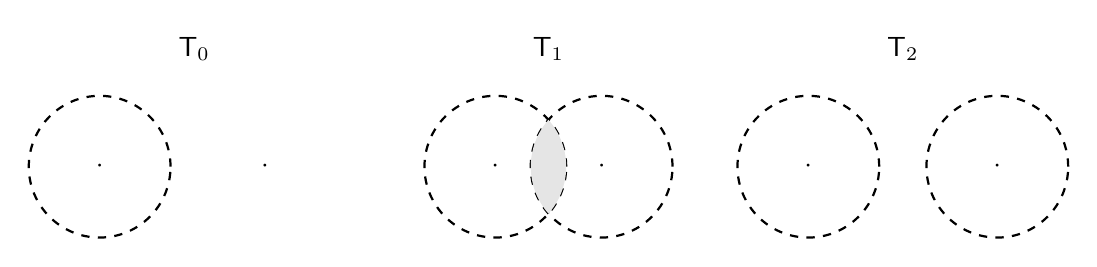
\begin{tikzpicture}[scale = 0.3]
		\draw[black,thick,dashed] (4,0) circle (3); 
		\node at (4,0) {$\cdot$};
		\node at (8,5) {$\mathsf{T}_0$};
		\node at (11,0) {$\cdot$};
		
		\draw[black,thick,dashed] (20.75,0) circle (3);
		\node at (20.75,0) {$\cdot$};
		\node at (23, 5) {$\mathsf{T}_1$};
		\draw[black,thick,dashed] (25.25,0) circle (3);
		\node at (25.25,0) {$\cdot$};
		
		\begin{scope}
			\clip (20.75,0) circle (3);
			\fill[black!10] (25.25,0) circle (3);
		\end{scope}
		
		\draw[black,thick,dashed] (34,0) circle (3);
		\node at (34,0) {$\cdot$};
		\node at (38,5) {$\mathsf{T}_2$};
		\draw[black,thick,dashed] (42,0) circle (3);
		\node at (42,0) {$\cdot$};
	\end{tikzpicture}
\end{center}

\begin{mathSection}
	\begin{defn}
		A topology for $X$ is \textbf{Kolmogorov} (or $\mathsf{T}_0$) if for every two elements $x_1, x_2 \in X$ there exists a verifiable set $U \in \mathsf{T}_X$ containing one element but not the other. That is: either $x_1 \in U$ while $x_2 \notin U$ or $x_1 \notin U$ while $x_2 \in U$.
	\end{defn}
	\begin{defn}
	A topology for $X$ is \textbf{Fr\'echet} (or $\mathsf{T}_1$) if for every two elements $x_1, x_2 \in X$ there exist two, not necessarily disjoint, verifiable sets $U_1, U_2 \in \mathsf{T}_X$ each containing only one element. That is: $x_1 
	\in U_1$ and $x_2 \in U_2$.
\end{defn}
	\begin{defn}
	A topology for $X$ is \textbf{Hausdorff} (or $\mathsf{T}_2$) if for every two elements $x_1, x_2 \in X$ there exist two disjoint verifiable sets $U_1, U_2 \in \mathsf{T}_X$ each containing one element. That is: $U_1 \cap U_2 = \emptyset$, $x_1 
	\in U_1$ and $x_2 \in U_2$.
\end{defn}
\begin{remark}
	Note that $\mathsf{T}_2$ implies $\mathsf{T}_1$ which in turn implies $\mathsf{T}_0$.
\end{remark}

\end{mathSection}

How do these properties relate to experimental domains? Consider two possibilities for a domain, for example \statement{that is a cat} and \statement{that is a swan}. We can always find a verifiable statement, such as \statement{that animal has feathers}, that we can use to distinguish one possibility from the other. This means that, given two different possibilities, we can always find a verifiable set that contains one and not the other: the natural topology for any set of possibilities is always $\mathsf{T}_0$.

Now suppose two possibilities are approximately verifiable as we defined in Definition \ref{def_approximately_verifiable}. For example, \statement{the mass of the photon is exactly 0 eV} or \statement{the mass of the photon is exactly $10^{-20}$ eV}. We can find two verifiable statements \statement{the mass of the photon is less than $10^{-25}$ eV} and \statement{the mass of the photon is more than $10^{-25}$ eV} each compatible with only one possibility. This means that, given two approximately verifiable possibilities, we can find two verifiable sets each containing only one possibility: if all possibilities are approximately verifiable then the natural topology is $\mathsf{T}_1$.

Now suppose two possibilities are experimentally distinguishable as we defined in Definition \ref{1_def_experimentally_distinguishable}. Then, by \ref{1_prop_experimentally_distinguishable_is_disjoint_approximations}, we can find two disjoint approximations. In the example before, the two verifiable statements were in fact incompatible. This means that, given two approximately verifiable possibilities, we can find two disjoint verifiable sets each containing only one possibility: if all possibilities experimentally distinguishable then the natural topology is $\mathsf{T}_2$.

\begin{mathSection}
	\begin{prop}
	The natural topology of a set of possibilities is Kolmogorov (or $\mathsf{T}_0$).
\end{prop}
\begin{proof}
	Let $X$ be the set of possibilities for an experimental domain $\edomain$. Let $x_1, x_2 \in X$ be two distinct possibilities. Each of them can be expressed as a minterm of a basis $\basis \subseteq \edomain$. Since the two possibilities are distinct, there must exist a verifiable statement $\stmt[e] \in \basis$ that appears negated in one conjunction but not the other. That is, $\stmt[e]$ is compatible with only one possibility. Since the verifiable set associated with a verifiable statement contains only the possibilities compatible with said statement, the verifiable set of $\stmt[e]$ either contains $x_1$ or $x_2$ but not both. The topology is therefore Kolmogorov (or $\mathsf{T}_0$).
\end{proof}
\begin{prop}
	The natural topology of a set of possibilities is Fr\'echet (or $\mathsf{T}_1$) if and only if all possibilities are approximately verifiable.
\end{prop}
\begin{proof}
	% TODO: Could be shorten since it is sufficient to just prove one side (I.e. given x,y in X, find U containing x but not y. No need to find another set for y. Because the points were arbitrary there is no loss of generality).
	Suppose all possibilities in $X$ for an experimental domain $\edomain_X$ are approximately verifiable. Let $x_1, x_2 \in X$ be two possibilities, then we can find two sequences of verifiable statements $\{\stmt_i^1\}_{i=1}^\infty, \{\stmt_j^2\}_{j=1}^\infty \in \edomain_X$ such that $x_1=\bigAND\limits_{i=1}^\infty \stmt_i^1$ and $x_2=\bigAND\limits_{j=1}^\infty \stmt_j^2$. We can assume the sequences are monotone with respect to narrowness, that is $\stmt_{i+1}^1 \narrower \stmt_i^1$, as we can always create a monotone sequence from one that is not by taking the sequence of finite conjunction, that is $\hat{\stmt}_k^1=\bigAND\limits_{i=1}^k \stmt_i^1$. If $x_1 \neq x_2$, then $x_1 \AND x_2 \equiv \impossibility$ since different possibilities are incompatible. Therefore we must have $x_1 \AND \stmt_j^2 \equiv \impossibility$ and $\stmt_i^1 \AND x_2 \equiv \impossibility$ from some $i,j \geq 1$ or the limits would not be incompatible. In terms of verifiable sets we have $x_2 \notin U(\stmt_i^1)$ and $x_1 \notin U(\stmt_j^2)$. For any two distinct possibilities we can find two verifiable sets each containing one: the natural topology is $\mathsf{T}_1$.

	Conversely, suppose the natural topology $\mathsf{T}_X$ for the possibilities $X$ for an experimental domain $\edomain_X$ is $\mathsf{T}_1$. Let $x \in X$ be a possibility. Consider the collection, not necessarily countable, of all verifiable sets $\{U_i\}_{i \in I} \subset \mathsf{T}_X$ such that they contain $x$. Consider their intersection $U_x = \bigcap\limits_{i \in I} U_i$. It will contain $x$ since all $U_i$ contain $x$. It will not contain anything else: since the topology is $\mathsf{T}_1$, for every other possibility $\hat{x}$ there is always an open set $U_i$ that does not contain it. Therefore $U_x = \{x\}$. Because the natural topology is second countable, we can find a countable basis $\basis$ and rewrite the arbitrary intersection into $\{x\} = \bigcap\limits_{i=1}^\infty V_i$ a countable intersection of elements $V_i \in \basis$ of the basis. Let $\{\stmt_i\}_{i=1}^\infty$ be the sequence of verifiable statements such that $U(\stmt_i) = V_i$ for every $i$. Then $x=\bigAND\limits_{i=1}^\infty \stmt_i$ which means $x$ is approximately verifiable.

\end{proof}
\begin{prop}
	The natural topology of a set of possibilities is Hausdorff (or $\mathsf{T}_2$) if and only if all possibilities are pairwise experimentally distinguishable.
\end{prop}
\begin{proof}
	Suppose all possibilities in $X$ for an experimental domain $\edomain_X$ are pairwise experimentally distinguishable. Then, by \ref{1_prop_experimentally_distinguishable_is_disjoint_approximations}, given two possibilities $x_1, x_2 \in X$ we can find two verifiable statements $\stmt_1, \stmt_2 \in \edomain_X$ such that $\stmt_1 \ncomp \stmt_2$, $x_1 \narrower \stmt_1$ and $x_2 \narrower \stmt_2$. In terms of verifiable sets we have $U(\stmt_1) \cap U(\stmt_2) = \emptyset$, $x_1 \in U(\stmt_1)$ and $x_2 \in U(\stmt_2)$. The topology is $\mathsf{T}_2$.
	
	Conversely, suppose the natural topology $\mathsf{T}_X$ for the possibilities $X$ for an experimental domain $\edomain_X$ is $\mathsf{T}_1$. Given two possibilities $x_1, x_2 \in X$ we can find two verifiable sets $U_1, U_2 \in \mathsf{T}_X$ such that $U_1 \cap U_2 = \emptyset$, $x_1 \in U_1$ and $x_2 \in U_2$. Since $U_1, U_2 \in \mathsf{T}_X$, we can find two corresponding verifiable statements $\stmt_1, \stmt_2 \in \edomain_X$ such that $U(\stmt_1) = U_1$ and $U(\stmt_2) = U_2$. We have $\stmt_1 \ncomp \stmt_2$, $x_1 \narrower \stmt_1$ and $x_2 \narrower \stmt_2$ and by \ref{1_prop_experimentally_distinguishable_is_disjoint_approximations} the possibilities are pairwise experimentally distinguishable.
\end{proof}
\end{mathSection}

\section{Sigma-algebras}

In the same way that experimental domains find a natural mathematical representation as topological spaces, theoretical domains find a natural mathematical representation in $\sigma$-algebras. The main result of this section is that a theoretical domain provides a natural $\sigma$-algebra on its possibilities.

Like topologies, $\sigma$-algebras are fundamental in mathematics as they allow us to construct measures (i.e.~assigning sizes to sets), limits for sequences of sets and probability spaces. It is again fitting that theoretical domains are associated to such a fundamental mathematical structure.

Let's first review what a $\sigma$-algebra is. The general idea is that we have a set $X$ of elements which we call points, and we have a collection of subsets of $X$ such that it is closed under complement and countable union, contains the empty set and contains the whole set $X$. For example, suppose $X = \{1,2,3\}$ then  $\{\{\},\{1\},\{1,2,3\}\}$ is not a $\sigma$-algebra while $\{\{\},\{1\}, \{2,3\},\{1,2,3\}\}$ is. The first one is missing the complement of $\{1\}$.

\begin{mathSection}
	\begin{defn}
		Let $X$ be a set. A \textbf{$\sigma$-algebra} on $X$ is a collection $\Sigma_X$ of subsets of $X$ closed under complement and countable union such that it contains $X$.
	\end{defn}
\end{mathSection}

Note that $\sigma$-algebras are also closed under countable intersections, since these can be expressed in terms of complements and countable unions.

In the previous section we saw how each verifiable statement can be expressed as the conjunction of a set of possibilities, how the operations on statements can be expressed as operations on the verifiable sets and how all the verifiable sets form a topology. The same is true for theoretical statements, with the only difference being that we will end up with a collection of sets that is closed under complement and countable union since the theoretical domain is closed under negation and countable disjunction.

\begin{mathSection}
	
	\begin{defn}
		Let $\tdomain$ be a theoretical domain and $X$ its possibilities. We define the map $A : \tdomain \rightarrow 2^X$ that for each theoretical statement $\stmt \in \tdomain$ returns the set of possibilities compatible with it. That is, $A(\stmt)\equiv\{ x \in X \, | \, x \comp \stmt\}$. We call $A(\stmt)$ the \textbf{theoretical set} of possibilities associated with $\stmt$
	\end{defn}
	
	\begin{prop}
		Let $X$ be the set of possibilities for a theoretical domain $\tdomain$. $X$ has a natural $\sigma$-algebra given by the collection of all theoretical sets $\Sigma_X=A(\tdomain)$.
	\end{prop}
	
	\begin{proof}
	The theoretical sets for the certainty and the impossibility correspond to the full set and empty set respectively. Formally, $A(\certainty) = \{ x \in X \, | \, x \comp \certainty\} = X$ while $A(\impossibility) = \{ x \in X \, | \, x \comp \impossibility\} = \emptyset$. Therefore $X, \emptyset \in A(\tdomain)$ since $\certainty, \impossibility \in \tdomain$.

	The complement of a theoretical set corresponds to the theoretical set of the negation and therefore it is a theoretical set. Formally, $A(\stmt)^C = \{ x \in X \, | \, x \ncomp \stmt\} =  \{ x \in X \, | \, x \comp \NOT\stmt\} = A(\NOT\stmt)$.

	The countable union of verifiable sets corresponds to the verifiable set of the countable disjunction and therefore it is a theoretical set. Formally, $A(\stmt_1\OR\stmt_2) = \{ x \in X \, | \, x \comp \stmt_1\OR\stmt_2\} =  \{ x \in X \, | \, x \comp \stmt_1 \, or \, x \comp \stmt_2\} = \{ x \in X \, | \, x \comp \stmt_1\} \cup \{ x \in X \, | \, x \comp \stmt_2\} = A(\stmt_1) \cup A(\stmt_2)$. This generalizes to countable disjunctions.

	The collection $\Sigma_X=A(\tdomain)$ is therefore a $\sigma$-algebra by definition since it satisfies all its properties.
	\end{proof}
\end{mathSection}

There is also a special link between topologies and $\sigma$-algebras. As one may want to construct measures and probability spaces on topological spaces, there is a standard way to construct a $\sigma$-algebra from a topology. This object, called Borel algebra, is the smallest $\sigma$-algebra that contains all verifiable sets defined by the topology. The $\sigma$-algebra defined by a theoretical domain is none other than the Borel algebra of the topology defined by the corresponding experimental domain.

\begin{mathSection}
	
	\begin{defn}
		Let $(X, \mathsf{T})$ be a topological space. Its \textbf{Borel algebra} is the collection $\Sigma_X$ of subsets of $X$ generated by countable union, countable intersection and complement from the verifiable sets.
	\end{defn}
	
	\begin{prop}
		The natural $\sigma$-algebra for a set of possibilities is the Borel algebra of its natural topology.
	\end{prop}
	
	\begin{proof}
		Since the theoretical domain can be generated by a basis of the experimental domain, the natural $\sigma$-algebra can be generated by a sub-basis of the natural topology. This means that it is also generated by countable union, countable intersection and negation from the verifiable sets of the natural topology.
	\end{proof}
\end{mathSection}

This fundamental link between experimental domains and topology on one side and theoretical domains and $\sigma$-algebra on the other is important for multiple reasons.

From a practical standpoint, it guarantees that these mathematical tools can always be used in science. Since experimental and theoretical domains are general constructs, any branch of scientific investigation can use techniques and results from topology and $\sigma$-algebras for calculations or for characterizing the domain at hand.

From a conceptual standpoint it provides a Rosetta stone, i.e a way to translate, between the mathematical concepts and the scientific ones. It gives a precise scientific meaning to the mathematical tools and everything built on top of them. Every single step in a calculation, every single argument in a proof can be given a clear, and possibly insightful, physical meaning. It grounds the abstract mathematical language in more concrete scientific objects. This in turn helps clarify the science described by common mathematical tools, unearthing possible hidden assumptions or simplifications about the physical systems being studied.

This connection explains why these mathematical tools have found such successful application in the physical sciences.

\section{Decidable domains}

We conclude this chapter by analyzing decidable domains, those for which we can experimentally test both the truth and the falsehood of all statements. For example, the domain for animal identification and the domain for the amount of money in my poket can be considered decidable as we can typically tell experimentally whether \statement{this animal has whiskers} or not, or whether \statement{there is more than one dollar and fifty cents in my pocket} or not.

Decidable domains have special characteristics and are easier to study. Since we can verify the negation, any theoretical statement is also verifiable. And since all theoretical statements are verifiable, so are the possibilities. That is, we can verify that \statement{this animal is a cat} and that \statement{there are two dollars and thirty cents in my pocket}. As all statements can be expressed as a disjunction of possibilities, the possibilities themselves form a countable basis. For example, \statement{there is more than one dollars and fifty cents in my pocket} can be expressed as the disjunction of the appropriate statements of the form \statement{there are x dollars and y cents in my pocket}.

\begin{mathSection}
\begin{defn}
	An experimental domain $\edomain_X$ is \textbf{decidable} if all statements in the domain are decidable. Formally, for every $\stmt \in \edomain_X$ we have $\NOT\stmt \in \edomain_X$.
\end{defn}

\begin{prop}\label{1_prop_decidable_domain_properties}
	Let $\edomain_X$ be an experimental domain. The following are equivalent:
	\begin{enumerate}
		\item the experimental domain is decidable
		\item the experimental domain and its theoretical domain coincide
		\item all possibilities are verifiable
		\item the possibilities form a countable basis.
	\end{enumerate}
\end{prop}

\begin{proof}
	To prove 2 from 1, suppose $\edomain_X$ is a decidable experimental domain. As $\edomain_X$ is decidable, it is already closed under negation and therefore all statements in its theoretical domain $\tdomain_X$ are already in $\edomain_X$.
	
	To prove 3 from 2, suppose $\edomain_X$ coincides with its theoretical domain $\tdomain_X$. As each possibility is a theoretical statement, it is also a verifiable statement.
	
	To prove 4 from 3, suppose the possibilities are verifiable. Note that the possibilities can generate all other statements through disjunction. To show $X$ is countable, consider a countable basis $\basis \subseteq \edomain_X$. Because the possibilities are verifiable statements, they can be generated from $\basis$ by finite conjunction and countable disjunction. Moreover, since the possibilities are the narrowest statements that are not impossible, they can be generated from $\basis$ using finite conjunction only. Since $\basis$ is countable and $X$ is generated by $\basis$ through finite conjunction, $X$ can be at most countable. Therefore $X$ is a countable basis.
	
	To prove 1 from 4, suppose the possibilities $X$ form a countable basis. Then each possibility is verifiable and so is their countable union. The negation of a verifiable statement can be expressed as the countable union of possibilities, and is therefore verifiable. All statements in the experimental domain are decidable and therefore the domain is decidable.
\end{proof}
\end{mathSection}

As the possibilities for a decidable domain must form a countable basis, their cardinality can't be greater than countable. That is: only domains that are non-decidable can have possibilities with cardinality of the continuum. In this sense they are more constrained and simpler to study.

Mathematically, the natural topology corresponds to the discrete topology: the one for which any subsets of the possibilities is a verifiable set. That is, the topology is simply the set of all possible sets of possibilities. The cardinality of the possibility is therefore enough to determine the topology of the space, which means that one number is enough to characterize the space.

\begin{mathSection}
\begin{defn}
	A topology $\mathsf{T}_X$ on a set $X$ is called \textbf{discrete} if it contains every subset of $X$.
\end{defn}

\begin{thrm}[Decidability is discreteness]\label{thrm_decidablity_is_discreteness}
	The natural topology of the possibilities $X$ for a domain $\edomain_X$ is discrete if and only if the domain is decidable.
\end{thrm}
\begin{proof}
	Suppose $\edomain_X$ is decidable. Let $U \subseteq X$ be a subset of possibilities. The statement $\stmt = \bigOR\limits_{x \in U} x$ is generated from $X$ through countable disjunction. Since $\edomain_X$ is decidable, $X$ is a countable basis and $\stmt$ is verifiable. Therefore $U$ is a verifiable set and it is contained in the natural topology. The natural topology of $X$ is discrete by definition.
	
	Now suppose $\edomain_X$ is such that the natural topology for its possibilities $X$ is discrete. Let $\stmt = \bigOR\limits_{x \in U} x$ be a statement. Since the topology is discrete, $U$ is part of the topology and $\stmt$ is verifiable. Consider its negation $\NOT\stmt = \bigOR\limits_{x \in U^C} x$. Since the topology is discrete, $U^C$ is also part of the topology and $\NOT\stmt$ is verifiable. This means $\stmt$ is decidable. Since every statement in $\edomain_X$ is decidable, the domain is decidable.
\end{proof}
	
\end{mathSection}

Note, though, that discrete does not imply finite or vice-versa. The domain for extra-terrestrial life is finite but is not decidable as we cannot verify that \statement{there is no extra-terrestrial life}. The domain for the amount of money in my pocket, instead, is decidable but not necessarily finite as I could potentially have an arbitrarily large amount.

\section{Summary}

In this first chapter we have laid down the foundations for our general mathematical theory of experimental science. We have seen how it is grounded in the logic of verifiable statements, which is more limited than the logic of pure statements as it has to deal with the practical constraints introduced by the termination of the tests.


\begin{center}
	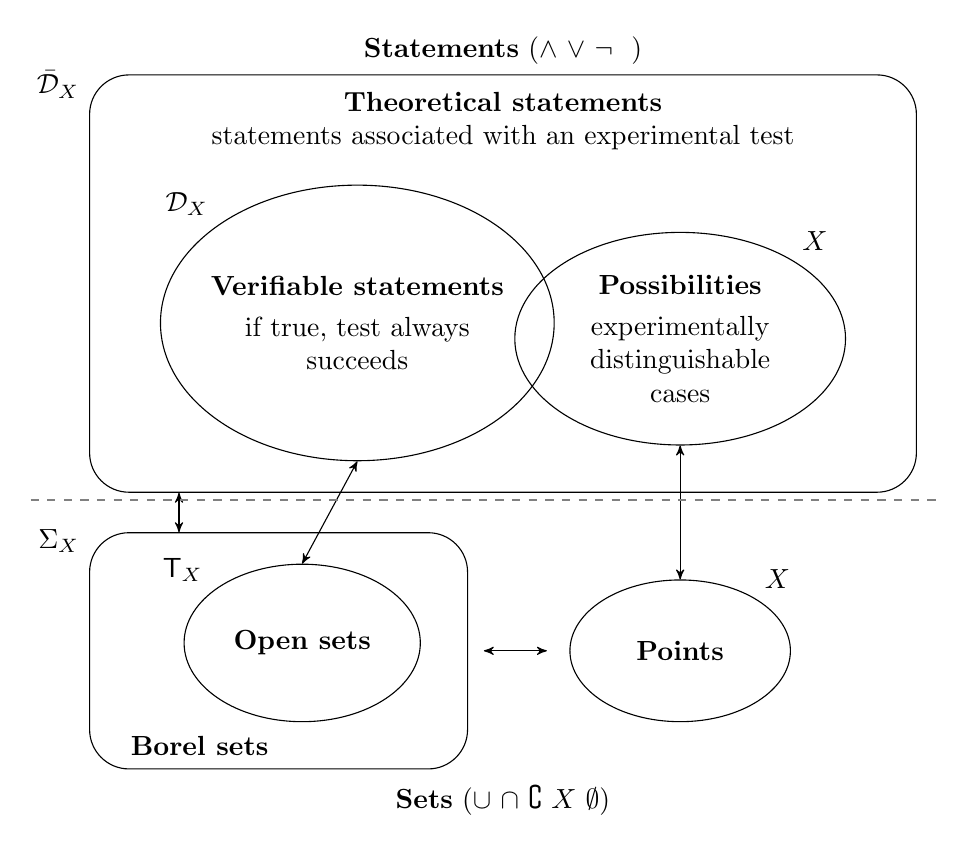
\begin{tikzpicture}
		\node[draw, minimum width=10.5cm, minimum height=5.3cm, rounded corners=5mm] (bdx) {};
		\node[align=center, below] at ([yshift=-1mm]bdx.north) {\textbf{Theoretical statements} \\statements associated with an experimental test};
		\node[align=center, above left] at (bdx.157) {$\tdomain_X$};
		\node[align=center, above] at (bdx.north) {\textbf{Statements} ($\AND$ $\OR$ $\NOT$ $\impossibility$ $\certainty$)};
		
		\node[ellipse, draw, minimum width=5cm, minimum height=3.5cm, align=center, inner xsep=-2mm] (vs) at ([xshift=-1.85cm, yshift=-5mm]bdx) {\textbf{Verifiable statements}\\[1mm]
			if true, test always\\
			succeeds};
		\node[align=center, above left] at (vs.145) {$\edomain_X$};
		\node[ellipse, draw, minimum width=4.2cm, minimum height=2.7cm, align=center,inner xsep=0mm] (poss) at ([xshift=2.25cm,yshift=-7mm]bdx) {\textbf{Possibilities}\\[1mm]
			experimentally\\
			distinguishable\\
			cases
		};
		\node[align=center, above right] at (poss.90-55) {$X$};
		
		\node[draw, minimum width=4.8cm, minimum height=3cm, rounded corners=5mm, anchor=north west] (sx) at ([yshift=-5mm]bdx.south west) {};
		\node[align=center, above] at ([xshift=-3mm,yshift=0.5mm]sx.-115) {\textbf{Borel sets}};
		\node[align=center, above left] at (sx.155) {$\Sigma_X$};
		
		\node[ellipse, minimum width=3cm, minimum height=2cm, draw] (os) at ([xshift=3mm,yshift=1mm]sx) {\textbf{Open sets}};
		\node[align=center, above left] at (os.150) {$\mathsf{T}_X$};
		\node[ellipse, minimum width=2.8cm, minimum height=1.8cm, draw] (point) at([yshift=-1mm]os-|poss)  {\textbf{Points}};
		\node[align=center, below=3.6cm] at (bdx.south) {\textbf{Sets} ($\cup$ $\cap$ $\complement$ $X$ $\emptyset$)};
		\node[align=center, above right] at (point.90-55) {$X$};
		
		\coordinate (z) at (bdx.south);
		\draw[stealth'-stealth'] (sx.130)--(z-|sx.130);
		\draw[stealth'-stealth'] (vs.south) to (os.90);
		\draw[stealth'-stealth'] (poss.south) to (point);
		\draw[stealth'-stealth'] ([xshift=2mm]sx.east)--+(8mm,0);
		
		\draw[gray, dashed, thick] (-6,-2.75)--+(11.5,0);
	\end{tikzpicture}
\end{center}


We saw that we can group verifiable statements into experimental domains which must have a countable basis to allow us to test any statement within an indefinite amount of time. We saw how to construct theoretical domains to find all the theoretical statements that we can use as predictions. And we saw how the possibilities are those statements that, if true, give a complete prediction for all statements in the domain.

We have seen that, because of the disjunctive normal form, each verifiable and theoretical statement is equivalent to a set of possibilities and how logic operations and relationships become set operations and relationships. As such, the experimental and theoretical domains respectively provide a natural topology and $\sigma$-algebra for the possibilities.

What we have ended up with is a conceptual framework that captures the necessary elements of scientific practice and codifies them into a symbolic representation with a well defined meaning. There is no guesswork as to what the points of our spaces are: they are the possibilities, statements that provide a complete prediction for the domain. We do not have to provide an ``interpretation" as to what the sets of a topology represent: they correspond to verifiable statements. All the objects have a clear definition and meaning from the start, we know which ones are necessary and to what extent they are physical or idealized. This will provide a much more solid foundation to the rest of the work, which will ultimately allow us to understand much better the fundamental physical theories and the connections between them and to other areas of scientific thought.



\newpage

\section{Reference sheet}

\begin{tabular}{p{0.2\textwidth} p{0.3\textwidth} p{0.5\textwidth}}
	& Name & Meaning  \\ 
	\hline 
	$\Bool$  & Boolean domain & the set of possible truth values \\ 
	&  & i.e.~$\Bool = \{\TRUE, \FALSE\}$ \\ 
	\hline 
	$\logCtx$ & logical context & a set of statements with well defined logical relationships \\ 
	\hline 
	$\stmt \in \logCtx$ & statement & an assertion with a well defined truth value \\ 
	\hline 
	$\truth : \logCtx \to \Bool$ & the truth function & returns whether a statement is true or not  \\ 
	\hline 
	$\pAss \subseteq \Bool^\logCtx$& possible assignments & the logically consistent truth value combinations that can be assigned to the statements \\ 
	\hline 
	$\certainty$ & certainty & a statement that can only be true (i.e.~it is true in all possible assignments) \\ 
	\hline 
	$\impossibility$ & impossibility & a statement that can never be true (i.e.~it is false in all possible assignments) \\ 
	\hline 
	& contingent statement & a statement that can be either true or false depending on the possible assignment \\ 
	\hline 
	$\NOT \stmt$ & negation (logical NOT) & the statement whose truth value is always opposite \\ 
	\hline 
	$\stmt_1 \AND \stmt_2$ & conjunction (logical AND) & the statement that is true only if all statements are true \\ 
	\hline 
	$\stmt_1 \OR \stmt_2$ & disjunction (logical OR) & the statement that is true if any of the statements is true \\ 
	\hline 
	$\stmt_1 \equiv \stmt_2$ & equivalence & whether each statement is a logical consequence of the other (i.e.~they must have the same value in every possible assignment) \\ 
	\hline 
	$\stmt_1 \narrower \stmt_2$ & narrower than & whether the first statement is more specific than the second (i.e.~in every possible assignment, if the first is true than the second must be also true) \\ 
	\hline 
	$\stmt_1 \broader \stmt_2$ & broader than & whether the second statement is narrower than the first \\ 
	\hline 
	$\stmt_1 \comp \stmt_2$ & compatibility & whether both statement can be true at the same time (i.e.~there is a possible assignment in which they are both true) \\
	\hline 
	$\stmt_1 \indep \stmt_2$ & independence & whether both statement can be true at the same time (i.e.~there is a possible assignment for each combination of their possible truths) \\
	\hline 
	& minterm & a conjunction where each statement appears once, either negated or not \\
	\hline 
	$\stmt \in \vstmtSet$ & verifiable statement & a statement that can be validated experimentally\\ 
	\hline 
	$\edomain$ & experimental domain & a set of verifiable statement that can be tested in an indefinite amount of time (i.e.~a set of statements closed under finite conjunction and countable disjunction, that precisely contains the certainty, the impossibility and a set of verifiable statements generated by a countable basis) \\ 
	\hline 
	$\basis \in \edomain$ & basis & a set of verifiable statements from which all others can be constructed\\ 
			
\end{tabular} 

\newpage

\begin{tabular}{p{0.2\textwidth} p{0.3\textwidth} p{0.5\textwidth}}
	& Name & Meaning  \\ 
	\hline 
	$\tdomain$ & theoretical domain & the set of all predictions for an experimental domain\\ 
	\hline 
	& approximately verifiable & when a statement is not verifiable but is the limit of a sequence of statements that are\\ 
	\hline 
	$X$ & possibilities of a domain & those predictions that sets the value of all verifiable statements of a domain\\ 
	\hline 
	$\estPoss$ & established possibility & a possibility for which at least a verifiable statements is true (i.e.~it can be established experimentally)\\ 
	\hline 
	$\resPoss$ & residual possibility & if it exists, the possibility for which all verifiable statements are false (i.e.~the remaining case that cannot be established experimentally)\\ 
	
\end{tabular} 


\chapter{Domain combination and relationships}

We continue our investigation of the fundamental mathematical structures for experimental science by studying what happens when we have more than one experimental domain. We will define \textbf{experimental relationships} between experimental domains, which capture either causal or inference relationships between them. We will see that these correspond to continuous functions in the natural topology.

We will take two or more domains and merge all the experimental information that can be gathered through them into a \textbf{combined domain}. We will study how the set of possibilities of the combined domain depends not only on the original domains, but also on the relationships between them. These will also determine the natural topology that can vary from the product topology all the way to the disjoint union topology.

We will also show that experimental relationships, under suitable conditions, can themselves be verified experimentally by constructing the \textbf{relationship domain} for which its possibilities correspond to the possible relationships.

\section{Dependence and equivalence between domains}

The first thing we want to be able to characterize, when dealing with more than one domain, is when there exists a relationship between them. For example, consider the domains for the temperature and height of a mercury column or the domains for the temperature and density of water. How do we express, in this framework, the fact that these domains are connected?

We have two ways to define these relationships between domains. The first is in terms of inference: any measurement on the height of a mercury column is an indirect measurement on its temperature; any experimental test on the density of water is an indirect experimental test on its temperature. The second is in terms of causes: the height of the mercury column depends on its temperature; the density of water is a function of its temperature. The main result of this section is to show that these definitions are equivalent and that the dependent domain can be seen as a sub-domain of the other.

Suppose $\edomain_X$ represents the domain for the temperature of a mercury column while $\edomain_Y$ represents the domain for its height. Since we know that an increase in temperature makes the metal expand, we can infer the temperature of the mercury column by looking at its height. For example, if we verify that \statement{the height of the mercury column is between 24 and 25 millimeters} we will be able to infer that \statement{the temperature is between 24 and 25 Celsius}. That is, given a verifiable statement $\stmt_Y$ we have another verifiable statement $\stmt_X$ that is going to be true if and only if the first one is, that is $\stmt_Y\equiv\stmt_X$.

Note that the inference is between verifiable statements and not intervals. For example, the verifiable statement \statement{the water density is between 999.8 and 999.9 kg/$m^3$} will correspond to \statement{the water temperature is between 0 and 0.52 Celsius}$\OR$\statement{the water temperature is between 7.6 and 9.12 Celsius} as water is most dense at 4 Celsius. The disjunction of verifiable statements is still a verifiable statement so we are still inferring one verifiable statement from the other. For each verifiable statement in $\edomain_Y$ we can find a verifiable statement in $\edomain_X$ that is verified if and only if the first is. That is: an inference relationship is a map from $\edomain_Y$ to $\edomain_X$ that preserves equivalence.

\begin{mathSection}
	\begin{defn}
		An \textbf{inference relationship} between two experimental domains establishes that testing a verifiable statement in one means testing a verifiable statement in the other. Formally, an inference relationship between two experimental domains $\edomain_X$ and $\edomain_Y$ is a map $\erel: \edomain_Y \to \edomain_X$ such that $\erel(\stmt_Y) \equiv \stmt_Y$. In other words: it is an equivalence-preserving map between experimental domains.
	\end{defn}
\end{mathSection}

An inference relationship is essentially an injection that preserves equivalence instead of identity. In terms of equality, the two statements \statement{the height of the mercury column is between 24 and 25 millimeters} and \statement{the temperature is between 24 and 25 Celsius} are different, but they are the same in terms of equivalence. In this sense, the dependent domain is already contained within the other domain. This means we can define domain inclusion and equivalence based on inference relationships.

\begin{mathSection}
	\begin{defn}
		An experimental domain $\edomain_Y$ is \textbf{dependent} on another experimental domain $\edomain_X$, noted $\edomain_Y \subseteq \edomain_X$, if there exists an inference relationship $\erel: \edomain_Y \to \edomain_X$.
	\end{defn}
	\begin{coro}\label{prop_domain_subset_is_dependence}
		Let $\edomain_X$ be an experimental domain. Let $\edomain_Y$ be a subset of statements of $\edomain_X$ that form an experimental domain (i.e. contains impossibility, certainty and is closed under finite conjunction and countable disjunction). Then $\edomain_Y \subseteq \edomain_X$.
	\end{coro}
	\begin{proof}
		Let $\iota : \edomain_Y \to \edomain_X$ be the inclusion map. This is an inference relationship since $\iota(\stmt_Y) = \stmt_Y \equiv \stmt_Y$ therefore $\edomain_Y$ depends on $\edomain_X$.
	\end{proof}
	\begin{defn}
		Two experimental domains $\edomain_X$ and $\edomain_Y$ are \textbf{equivalent} $\edomain_X \equiv \edomain_Y$ if $\edomain_X$ depends on $\edomain_Y$ and vice-versa.
	\end{defn}
	\begin{coro}
		Domain equivalence satisfies the following properties:
		\begin{itemize}
			\item reflexivity: $\edomain \equiv \edomain$
			\item symmetry: if $\edomain_X \equiv \edomain_Y$ then $\edomain_Y \equiv \edomain_X$
			\item transitivity: if $\edomain_X \equiv \edomain_Y$ and $\edomain_Y \equiv \edomain_Z$ then $\edomain_X \equiv \edomain_Z$
		\end{itemize}
		and is therefore an \textbf{equivalence relationship}.
	\end{coro}
	\begin{proof}
		For reflexivity, $\edomain$ is a subset of $\edomain$ that is an experimental domain, therefore $\edomain \subseteq \edomain$ by \ref{prop_domain_subset_is_dependence}. Equivalence follows by symmetry.
		
		For symmetry, suppose $\edomain_X \equiv \edomain_Y$, then $\edomain_Y \subseteq \edomain_X$ and $\edomain_X \subseteq \edomain_Y$ and therefore $\edomain_Y \equiv \edomain_X$.
		
		For transitivity, suppose $\edomain_X \equiv \edomain_Y$ and $\edomain_Y \equiv \edomain_Z$. Then we have the following inference relationships: $\erel_{XY} : \edomain_X \to \edomain_Y$, $\erel_{YX} : \edomain_Y \to \edomain_X$, $\erel_{YZ} : \edomain_Y \to \edomain_Z$, $\erel_{ZY} : \edomain_Z \to \edomain_Y$. We can define the function compositions $\erel_{XZ} = \erel_{YZ} \circ \erel_{XY}$ and $\erel_{ZX} = \erel_{YX} \circ \erel_{ZY}$. These are inference relationships since $\stmt_X \equiv \erel_{XY}(\stmt_X) \equiv \erel_{YZ}(\erel_{XY}(\stmt_X))$ and $\stmt_Z \equiv \erel_{ZY}(\stmt_Z) \equiv \erel_{YX}(\erel_{ZY}(\stmt_Z))$. Therefore $\edomain_X \equiv \edomain_Z$.
	\end{proof}
\end{mathSection}


\begin{center}
	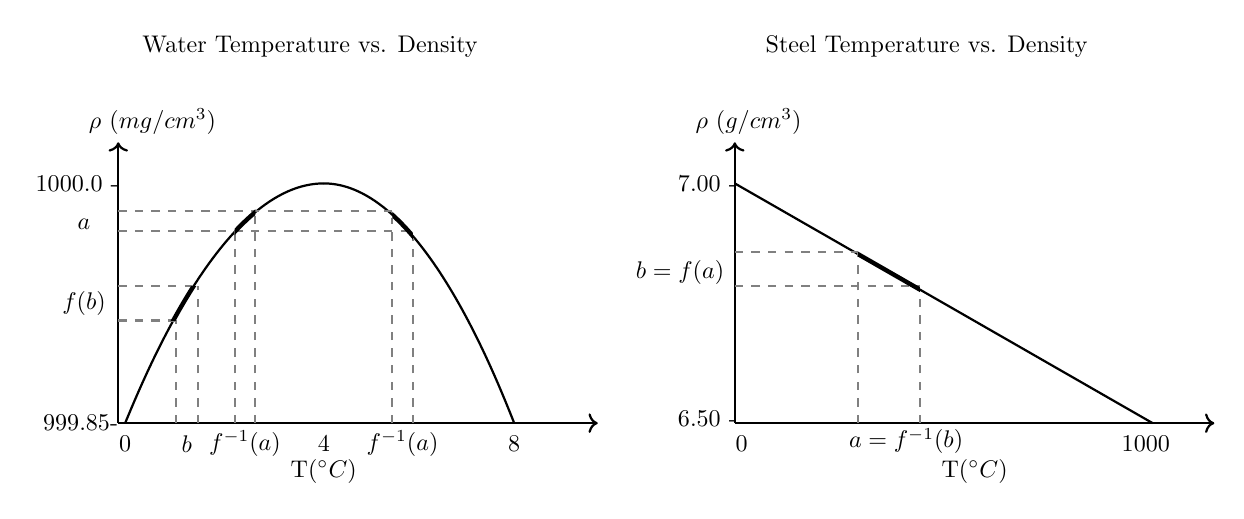
\begin{tikzpicture}[thick,scale=0.87, every node/.style={scale=0.87}]
		
		\draw[thick,->] (-1,3) -- (6,3);
		\draw[thick,->] (-1,3) -- (-1,7.1);
		
		\node at (-0.5,7.4) {$\rho$ ($mg/cm^3$)};
		\node at (2,2.3) {T($^\circ C$)};
		
		\node at (2,2.7) {4};
		\node at (4.78,2.7) {8};
		\node at (-0.9,2.7) {0};
		
		\node at (-1.6,6.5) {1000.0 -};
		\node at (-1.55,3.01) {999.85-};
		
		
		\draw (2,6.5) parabola (4.78,3);
		\draw (2,6.5) parabola (-0.9,3);
		
		\draw[gray,thick,dashed] (-1,4.5) -- (-0.16,4.5);
		\draw[gray,thick,dashed] (-1,5) -- (0.1,5);
		
		\draw[gray,thick,dashed] (-0.16,3) -- (-0.16,4.5);
		\draw[gray,thick,dashed] (0.16,3) -- (0.16,5);
		
		\node at (0,2.7) {$b$};
		\node at (-1.5,4.75) {$f(b)$};
		
		
		\draw[gray,thick,dashed] (0.7,3) -- (0.7,5.8);
		\draw[gray,thick,dashed] (1,3) -- (1,6.1);
		
		\draw[gray,thick,dashed] (-1,5.8) -- (3.25,5.8);
		\draw[gray,thick,dashed] (-1,6.1) -- (3,6.1);
		
		\draw[gray,thick,dashed] (3,3) -- (3,6);
		\draw[gray,thick,dashed] (3.3,3) -- (3.3,5.7);
		
		\node at (0.85,2.7) {$f^{-1}(a)$};
		\node at (3.15,2.7) {$f^{-1}(a)$};
		\node at (-1.5,5.9) {$a$};
		
		\begin{scope}
			\clip (-0.5,4.5) rectangle (0.2,5);
			\draw[black, ultra thick] (2,6.5) parabola (-0.9,3);
		\end{scope}
		
		\begin{scope}
			\clip (0.7,5.2) rectangle (1,6.5);
			\draw[black, ultra thick] (2,6.5) parabola (-0.9,3);
		\end{scope}
		
		\begin{scope}
			\clip (3,5) rectangle (3.3,6.3);
			\draw[black, ultra thick] (2,6.5) parabola (4.78,3);
		\end{scope}
		
		
		\draw[thick,->] (8,3) -- (15,3);
		\draw[thick,->] (8,3) -- (8,7.1);
		
		\node at (11.5,2.3) {T($^\circ C$)};
		\node at (8.2,7.4) {$\rho$ ($g/cm^3$)};
		
		\draw (8,6.5) -- (14.1,3);
		
		\node at (7.6,6.5) {7.00 -};
		\node at (7.6,3.06) {6.50 -};
		\node at (14,2.7) {1000};
		\node at (8.1,2.7) {0};
		
		\draw[gray,thick,dashed] (8,5.5) -- (9.8,5.5);
		\draw[gray,thick,dashed] (8,5) -- (10.7,5);
		
		\draw[gray,thick,dashed] (9.8,3) -- (9.8,5.5);
		\draw[gray,thick,dashed] (10.7,3) -- (10.7,4.9);
		
		\begin{scope}
			\clip (9.8,4.5) rectangle (10.7,5.5);
			\draw[black, ultra thick] (8,6.5) -- (14.1,3) ;
		\end{scope}
		
		
		\node at (10.5,2.74) {$a=f^{-1}(b)$};
		\node at (7.2,5.2) {$b=f(a)$};
		
		
		\node at (1.8,8.5) {Water Temperature vs. Density};
		\node at (10.8,8.5) {Steel Temperature vs. Density};
	\end{tikzpicture}
\end{center}


It should be evident that we cannot impose inference relationships between any two domains: it's something that the domains allow or not. The domains for the temperature of two different mercury columns are in general not related: testing the value of one does not tell us anything about the other. The topologies of the two domains, however, are going to be the same because we'll have the same possible values and the same way to experimentally test them. Equivalence between experimental domains is a much stronger relationship than equivalence of the natural topology. It carries enough of the semantic to be able to tell what spaces are truly scientifically equivalent.

Let's continue with our example. We can re-express a relationship between domains in terms of causal relationship between the two domains. If $x$ is the value of temperature of the mercury column (i.e. a possibility for $\edomain_X$) and $y$ is the height of the mercury column (i.e. a possibility for $\edomain_Y$), then we can write $y=f(x)$ since the height is determined by the temperature.

Note that the direction of the causal relationship is the opposite of the inference. $X$ causes $Y$ and from $\edomain_Y$ we can infer $\edomain_X$ . Chains of events are in terms of possibilities and start with the cause and end with the effect. Chains of inferences are in terms of verifiable statements and start with the result and end with the origin.

The other directions do not work in general. Even if we know the final possibility, we may not be able to reconstruct the initial possibility: if the water density is exactly 999.9 kg/$m^3$, the temperature could be either 0.52 or 7.6 Celsius because density peaks at 4 Celsius. For the same reason, a measurement of the cause is not always equivalent to a measurement of the effect: verifying that \statement{the water temperature is between 0 and 0.52 Celsius} will mean that \statement{the water density is between 999.8 and 999.9 kg/$m^3$} but not the other way around. Because of the peak in density, the statement about the temperature tells us more (i.e. it is narrower) than the statement about the density and therefore they are not equivalent. That is: we can learn more about the temperature by measuring it directly than indirectly through the density.

Another important consideration is that, in order to be consistent, the function $y=f(x)$ has to be continuous. The general idea is the following: if we say that we can only measure both the temperature and height of a mercury column with finite precision, we have to make sure that we can use the causal relationship for inference. Therefore a finite precision measurement of height will correspond to a finite precision measurement of temperature. This means a small change in height has to correspond to a small change in temperature: the function is continuous.

More precisely, consider the verifiable statement $\stmt_Y=$\statement{the height of the mercury column is between 24 and 25 millimeters}. The height of the mercury column $y$ is within the verifiable set $U(\stmt_Y) = (24, 25)$ millimeters. We can then infer that the temperature must be in the reverse image of the possible heights $f^{-1}(U_Y(\stmt_Y))=(24,25)$ Celsius. But this means that, indirectly, we have experimentally verified that $x$ is in $f^{-1}(U_Y(\stmt_Y))$. And if $\edomain_X$ is really the domain of the verifiable statements for the temperature, then it must contain one that matches \statement{the temperature of the mercury column is between 24 and 25 Celsius}. In other words, $f^{-1}(U_Y(\stmt_Y))$ must be a set in the topology of $X$ and the function is continuous.\footnote{In topology, continuity is defined in terms of the sets in the topology and not in terms of small changes as in analysis. When using the standard topology on real numbers, the two coincide but not in general.}

\begin{mathSection}
	\begin{defn}
		Let $(X, \mathsf{T}_X)$ and $(Y, \mathsf{T}_Y)$ be two topological spaces. A \textbf{continuous function} is a map $f: X \to Y$ such that given any verifiable set $U_Y \in \mathsf{T}_Y$ its reverse image $f^{-1}(U_Y) \in \mathsf{T}_X$ is a verifiable set. A \textbf{homeomorphism} is a continuous bijective map such that its inverse is also continuous.
	\end{defn}
	\begin{defn}
		A \textbf{causal relationship} between two experimental domains establishes that determining which possibility is true in the first domain also determines which possibility is true in the second. Formally, a causal relationship between two experimental domains $\edomain_X$ and $\edomain_Y$ is a function $f : X \to Y$ between the possibilities of the respective domains such that $x \narrower f(x)$ for all $x \in X$.
	\end{defn}
	\begin{coro}
		All causal relationships are continuous functions over the respective natural topologies.
	\end{coro}
	\begin{proof}
		Let $f : X \to Y$ be a causal relationship between $\edomain_X$ and $\edomain_Y$. Let $y \in Y$ be a possibility for $\edomain_Y$. Consider $f^{-1}(y)$: this is the set of all possibilities in $X$ that are compatible with $y$ which is, by definition, the theoretical set of $y$. Therefore we have $y \equiv \bigOR\limits_{x \in f^{-1}(y)} x$. Now consider a verifiable statement $\stmt_Y \in \edomain_Y$ and the associated verifiable set $U_Y(\stmt_Y) \subseteq Y$. We have $\stmt_Y \equiv \bigOR\limits_{y \in U_Y(\stmt_Y)} y \equiv \bigOR\limits_{y \in U_Y(\stmt_Y)} \bigOR\limits_{x \in f^{-1}(\{y\})} x \equiv \bigOR\limits_{x \in f^{-1}(U_Y(\stmt_Y))} x$. Given that $\stmt_Y$ is verifiable, $\bigOR\limits_{x \in f^{-1}(U_Y(\stmt_Y))} x$ is also verifiable because it is equivalent to a verifiable statement. Since $f^{-1}(U_Y(\stmt_Y))$ is the set of possibilities compatible with that statement, $f^{-1}(U_Y(\stmt_Y))$ must be a verifiable set and therefore $f^{-1}(U_Y(\stmt_Y)) \in \mathsf{T}_X$ must be in the natural topology of $\edomain_{X}$. Therefore $f$ is a continuous function over the respective natural topologies.
	\end{proof}
	\begin{coro}
		A causal relationship between two domains is unique if it exists.
	\end{coro}\label{prop_causal_relationship_unique}
	\begin{proof}
		Suppose $f_1 : X \to Y$ and $f_2 : X \to Y$ are two causal relationships. Let $x \in X$. We have $x \narrower f_1(x)$ and $x \narrower f_2(x)$. This means $f_1(x) \comp f_2(x)$. But these are two possibilities of the same domain, so they are either incompatible or are the same possibilities. Therefore $f_1(x) \equiv f_2(x)$ for all $x \in X$. The causal relationships are the same.
	\end{proof}
	\begin{thrm}[Experimental Relationship Theorem]\label{2_thrm_experimental_relationship}
		Inference and causal relationships are equivalent. More formally, let $\edomain_X$ and $\edomain_Y$ be two experimental domains. An inference relationship $\erel: \edomain_Y \to \edomain_X$ exists between them if and only if a causal relationship $f: X \to Y$ also exists.
	\end{thrm}
	\begin{proof}
		First we show that a causal relationship exists between the independent and the dependent domain. Suppose $\edomain_Y$ depends on $\edomain_X$. Given that for each statement in $\edomain_Y$ there exists an equivalent statement in $\edomain_X$, $\edomain_Y$ is effectively a subset of $\edomain_X$. Moreover, since the theoretical domains for both experimental domains are generated by completing under negation, the theoretical domain $\tdomain_Y$ will effectively be a subset of $\tdomain_X$. This means that a possibility $x \in \tdomain_X$, if true, will determine all the truth values of  all statements in $\tdomain_Y$, including its possibilities. Because one possibility of $Y$ must be true and because all possibilities are incompatible with each other, there must be one and only one possibility $y \in \tdomain_Y$ compatible with $x$. Therefore we can define $f : X \to Y$ the function that given a possibility $x \in X$ returns the only possibility $y=f(x) \broader x$ that is compatible with it.
		
		We still need to show that $f$ is continuous. Consider a verifiable statement $\stmt_Y \in \edomain_Y$. Let $U_Y(\stmt_Y) \in \mathsf{T}_Y$ be its verifiable set. Since $\edomain_Y$ depends on $\edomain_X$, we can find $\stmt_X \in \edomain_X$ such that $\stmt_X \equiv \stmt_Y$. Let $U_X(\stmt_X) \in \mathsf{T}_X$ be its verifiable set. This is also the set of all possibilities in $X$ that are compatible with $\stmt_Y$, which means $U_X(\stmt_X)$ contains all the possibilities that are compatible with a possibility in $U_Y(\stmt_Y)$. Since $f$ returns the only possibility in $Y$ compatible with a possibility in $X$, $f^{-1}(U_Y(\stmt_Y))$ will return all the possibilities in $X$ that are compatible with a possibility in $U_Y(\stmt_Y)$. That means $f^{-1}(U_Y(\stmt_Y)) = U_X(\stmt_X)$ and that $f^{-1}$ maps verifiable sets to verifiable sets. Therefore $f$ is continuous.
		
		Now we show that a causal relationship implies dependence between domains. Suppose we have a causal relationship $f: X \to Y$ between $\edomain_X$ and $\edomain_Y$. Let $y \in Y$ be a possibility for $\edomain_Y$. Consider  $f^{-1}(\{y\})$: this is the set of all possibilities in $X$ that are compatible with $y$ which is, by definition, the theoretical set of $y$. Therefore we have $y \equiv \bigOR\limits_{x \in f^{-1}(\{y\})} x$. Now consider a verifiable statement $\stmt_Y \in \edomain_Y$. We have $\stmt_Y \equiv \bigOR\limits_{y \in U_Y(\stmt_Y)} y \equiv \bigOR\limits_{y \in U_Y(\stmt_Y)} \bigOR\limits_{x \in f^{-1}(\{y\})} x \equiv \bigOR\limits_{x \in f^{-1}(U_Y(\stmt_Y))} x$. Because $f$ is continuous, the reverse image of a verifiable set is a verifiable set. Therefore there is an $\stmt_X \in \edomain_X$ such that $U_X(\stmt_X) = f^{-1}(U_Y(\stmt_Y))$. The two verifiable statements $\stmt_X \equiv \bigOR\limits_{x \in U_X(\stmt_X)} x \equiv \stmt_Y$ are equivalent. For each $\stmt_Y \in \edomain_Y$ we can find an equivalent $\stmt_X \in \edomain_X$ so $\edomain_Y$ depends on $\edomain_X$.
	\end{proof}

\begin{coro}
	Two experimental domains $\edomain_{X}$ and $\edomain_{Y}$ are equivalent if and only if there exists a homeomorphism $f : X \to Y$ between the possibilities such that $x \equiv f(x)$.
\end{coro}
\begin{proof}
	Let $\edomain_{X}$ and $\edomain_{Y}$ be two equivalent experimental domains. Then we can find the causal relationship $f : X \to Y$ and $g : Y \to X$. We have $x \narrower f(x) \narrower g(f(x))$. Since $g(f(x)) \in X$ is a possibility, and since $x$ is the only possibility compatible with itself, we must have $x \equiv g(f(x))$. Therefore $g$ is the inverse of $f$ and it is continuous. Therefore $f$ is a homeomorphism. We also have $x \narrower f(x) \narrower x$, therefore $f(x) \equiv x$.
	
	Now let $f : X \to Y$ be a homeomorphism between the possibilities of $\edomain_{X}$ and $\edomain_{Y}$ such that $x \equiv f(x)$. Then $f$ is a causal relationship and $\edomain_{Y}$ depends on $\edomain_{X}$. Let $g$ be the inverse of $f$, which is continuous since $f$ is a homeomorphism. We have $y \equiv f(g(y)) \equiv g(y)$. Then $g$ is also a causal relationship and $\edomain_{X}$ depends on $\edomain_{Y}$. Therefore $\edomain_{X} \equiv \edomain_{Y}$.
\end{proof}
\end{mathSection}

Since for each inference relationship we have a causal relationship and vice-versa, we will simply use the term \textbf{experimental relationship} to describe the link between the two domains.

We should stress that causal relationships and inference relationships are defined on spaces that have, in a sense, a different status in a physical theory. Inference relationships are defined on verifiable statements, on finite precision measurements, which are the objects that are directly defined experimentally. In this sense, inferences have a higher status as they are more directly related to experimental verification. However, the map $\erel : \edomain_Y \to \edomain_X$ is over-complicated and redundant precisely because it maps all possible finite precision measurements from one domain to the other. Conversely, the causal relationship $f : X \to Y$ is only defined on the possibilities, on the points, therefore there is no redundancy. However, the possibilities are not verifiable statements in general and are often the product of idealizations. In this sense, causal relationships have a lower status as they are only indirectly defined by experimental verification.

The perfect correspondence between causal and inference relationships is what rescues and justifies the predominant focus on causal relationships to describe experimental relationships: since studying one is mathematically the same as studying the other, why should we use the more complicated object? Therefore, while the inference relationship is more directly physically meaningful, the causal relationship is a much more convenient object to study and characterize. That is why, in the end, all relationships will be predominantly defined by a function over the possibilities.

We now turn our attention back to domain equivalence. We have seen that two experimental domains $\edomain_X$ and $\edomain_Y$ are equivalent if they consist of equivalent statements: if they allow a one to one correspondence that preserves the equivalence of their statements. This implies, for example, that the possibilities are also equivalent but there is more to it.

Suppose we define some type of operation on one domain. For example, on the experimental domain for the temperature of a mercury column we define an increase by one Celsius; or on the experimental domain for the amount of gasoline in a tank we define the sum of two possible amounts. These will correspond either to operations on the domain (e.g. $f : \edomain_X \to \edomain_X$) or on its possibilities (e.g. $+ : X \times X \to X$). But by doing so we are also defining them on all equivalent domains as well: in the end, they are made of equivalent statements. Therefore we are also defining an increase of the height of the mercury column and the sum of the monetary value of the gasoline.

This means that if we capture some physical feature using some mathematical structure on one domain, then all equivalent domains will inherit the same structure. Moreover, the causal relationship is a function that preserves that structure. If the possibilities of one domain form a vector space, then the possibilities of an equivalent domain form a vector space and the causal relationship is an invertible linear transformation. If the possibilities of one domain form a group, then the possibilities of an equivalent domain form a group and the causal relationship is an isomorphism.\footnote{Domain equivalence is an isomorphism in whatever category (e.g. topological space, group, vector space, ...) used to model the experimental domain.} As we'll see much later, this is fundamental since deterministic and reversible evolution means equivalence of the domains describing the past, present and future states. Therefore deterministic and reversible motion is not ``just" a one to one map.

\begin{mathSection}
	\begin{thrm}[Domain Equivalence is Isomorphism]\label{thrm_domain_equivalence_is_isomorphism}
		Let $\edomain_Y \equiv \edomain_X$ be two equivalent experimental domains. Suppose $\edomain_X$ is endowed with some mathematical structure. Then $\edomain_Y$ is also endowed with an equivalent structure and the experimental relationship preserves said structure.
	\end{thrm}
\begin{proof}
	Since an experimental domain is really defined not on the statements themselves but on their equivalence classes, the mathematical structure will also be defined on the equivalence classes. But this means that a structure defined on $\edomain_X$ is also defined on $\edomain_Y$ since they contain the same equivalence classes. Therefore $\edomain_Y$ is also endowed with an equivalent structure.
	
	The experimental relationship can either expressed as a map between possibilities $f : X \to Y$ or as a map between verifiable statements $\erel : \edomain_X \to \edomain_Y$. This means that the mathematical structure defined on $\edomain_Y$ can be transported to $\edomain_X$ using the experimental relationship. But since the mathematical structure defined on $\edomain_X$ already contains the mathematical structure defined on $\edomain_Y$, the transported mathematical structure has to be the same. That is, the experimental relationship must preserve the mathematical structure defined on $\edomain_X$.
\end{proof}
\end{mathSection}

Note that the converse is not true: two domains that are endowed with the same mathematical structure are not necessarily equivalent. Consider two similarly constructed thermometers: their respective experimental domains are not equivalent since knowing something about one tells us nothing about the other. Yet, their natural topologies are equivalent because the way we can measure temperature for both is the same. One way to look at it is that the mathematical structures ``forget" the full equivalence between statements and only look at a particular aspect. Topological spaces capture how the possibilities are distinguished in terms of verifiable statements. Therefore, while the domains for temperature of two different thermometers are not equivalent, their natural topologies are equivalent because the way we characterize all possible measurements is the same (i.e. the value is within a finite precision interval). Similarly, the $\sigma$-algebra only cares about what statements lead to valid predictions. We'll see that, in some cases, Abelian groups will capture how distributions can be composed into other distributions, that non-Abelian groups will capture how transformations can be composed into other transformations, and so on.

\section{Combining domains}

In this section we want to understand what happens when we combine statements from different domains. For example, suppose we have the experimental domain for the pressure of an ideal gas and the experimental domain for its temperature. We can mix and match verifiable statements with conjunction and disjunction as in \statement{the pressure is between 1 and 1.1 KPa}$\AND$\statement{the temperature is between 20 and 21 C} creating a new domain. How can we characterize this combined experimental domain?

The main result of this section is that the possibilities of the combined domain depend on how compatible the verifiable statements of the domains are. In particular, if the verifiable statements are independent across domains (e.g. the horizontal and vertical position of an object), then the possibilities of the combined domain will be the scalar product of those for the individual domains. On the other hand, if the verifiable statements are incompatible across domains (e.g. plant identification and animal identification), then the possibilities for the combined domain will be the disjoint union of the possibilities of the individual domains.

Suppose $\edomain_X$ is the experimental domain generated by the two verifiable statements \statement{the patient is dead} and \statement{the patient is alive} and a second one $\edomain_Y$ generated by the two verifiable statements \statement{the patient is not in a coma} and \statement{the patient is in a coma}. The given verifiable statements also correspond to the possibilities for the respective domains.

We can construct the combined domain $\edomain_X \times \edomain_Y$ by taking all possible disjunctions and conjunctions. What are the possibilities for the new domain? Since by \ref{prop_poss_is_minterm} the possibilities are minterms, we have the following cases to consider:
\begin{itemize}
	\item \statement{the patient is alive} $\AND$ \statement{the patient is in a coma}
	\item \statement{the patient is alive} $\AND$ \statement{the patient is not in a coma}
	\item \statement{the patient is dead} $\AND$ \statement{the patient is in a coma}
	\item \statement{the patient is dead} $\AND$ \statement{the patient is not in a coma}
\end{itemize}
The third one is impossible: the patient cannot be dead and in a coma. Therefore the combined domain has only three possibilities. The possibilities of the combined domain are, in general, the subset of all possible combinations (i.e. the scalar product) of the possibilities of the domains we are combining, those that are not impossible.

\begin{mathSection}
%TODO: Choose a different symbols for domain combination. Introduce somewhere "projections" as maps between domains. Show that domain combination is both the product and coproduct.
	
	\begin{defn}
		Let $\{\edomain_{X_i}\}_{i=1}^{\infty}$ be a countable set of experimental domains. The \textbf{combined experimental domain} $\edomain_{X} = \bigtimes\limits_{i=1}^{\infty} \edomain_{X_i}$ is the experimental domain generated from all statements in $\{\edomain_{X_i}\}_{i=1}^{\infty}$ by finite conjunction and countable disjunction.
	\end{defn}
	\begin{proof}
		We need to show that the combined experimental domain is indeed an experimental domain. It will contain the certainty and the impossibility since any of the original experimental domains contains them. It is closed under finite conjunction and countable disjunction by construction. To show that it has a countable basis, for each $i=1..\infty$ let $\basis_i \in \edomain_{X_i}$ be a countable basis for the respective domain. Consider $\basis=\bigcup\limits_{i=1}^\infty \basis_i$. From this set we can generate any $\edomain_{X_i}$ and therefore we can also generate all of $\edomain_{X}$. $\basis$ is a basis and it is countable since it is the union of a countable set of countable elements. Note that it is precisely because the basis needs to remain countable that we cannot extend the operation to an uncountable set of domains.
	\end{proof}
	
	\begin{prop}\label{prop_combined_possibility}
		The possibilities for a combined domain are a subset of the scalar product of the possibilities for the individual domains. Formally, let $\{\edomain_{X_i}\}_{i=1}^{\infty}$ be a countable set of experimental domains and $\{X_i\}_{i=1}^{\infty}$ their respective possibilities. Let $X$ be the set of possibilities for the combined domain $\edomain_{X} = \bigtimes\limits_{i=1}^{\infty} \edomain_{X_i}$.  Then $X = \{ x = \bigAND\limits_{i=1}^{\infty} x_i \, | \, \{x_i\}_{i=1}^{\infty} \in \bigtimes\limits_{i=1}^{\infty} X_i, \, x \nequiv \impossibility \}$.
	\end{prop}   
	\begin{proof}
		A possibility $x$ of the combined domain is a minterm of a basis $\basis \subseteq \edomain_{X}$. Since we can choose $\basis=\bigcup\limits_{i=1}^\infty \basis_i$ where $\basis_i \subseteq \edomain_{X_i}$ is a countable basis for each domain, $x$ is the conjunction $x \equiv \bigAND\limits_{i=1}^{\infty}x_i$ of minterms $x_i$ of $\basis_i$. Since $x$ is a possibility, it is not impossible and therefore none of the $x_i$ can be impossible. Since each $x_i$ is a minterm of the respective basis $\basis_i$ that is not impossible, it is a possibility by \ref{prop_poss_is_minterm}. Therefore a possibility $x$ of the combined domain is the conjunction of the possibilities $x_i$ of the original domains that is not impossible.
	\end{proof}

	\begin{prop}
		Let $\{\edomain_{X_i}\}_{i=1}^{\infty}$ be a countable set of incomplete experimental domains and $\edomain_X$ their combined experimental domain. Let $\{\resPoss_i\}_{i=1}^{\infty}$ be  the residual possibility of each respective domain. Let $\resPoss = \bigAND\limits_{i=1}^{\infty} \resPoss_i$. The combined domain $\edomain_X$ is incomplete if and only if $\resPoss \nequiv \impossibility$ in which case $\resPoss$ is the residual possibility.
	\end{prop}
	
	\begin{proof}
		For each domain, the residual possibility is the conjunction of the negation of its basis. Therefore we have $\resPoss \equiv \bigAND\limits_{\stmt[e] \in \basis} \NOT \stmt[e] \equiv \bigAND\limits_{i=1}^{\infty} \bigAND\limits_{\stmt[e] \in \basis_i} \NOT \stmt[e] \equiv \bigAND\limits_{i=1}^{\infty} \resPoss_i$. If $\resPoss \nequiv \impossibility$ then it is the residual possibility.
	\end{proof}
	
	\begin{coro}
		The residual possibility of the combined domain is narrower than the ones of the original domains. If one of the domains is complete then the combined domain is also complete.
	\end{coro}

	\begin{proof}
		Let $\resPoss$ be the residual possibility for the combined domain and $\resPoss_j$ the one for one of the original domains. We have $\resPoss_j \AND \resPoss \equiv \resPoss_j \AND \bigAND\limits_{i=1}^{\infty} \resPoss_i \equiv \bigAND\limits_{i=1}^{\infty} \resPoss_i \equiv \resPoss$. Therefore, by \ref{prop_narrowness_properties} $\resPoss \narrower \resPoss_j$.
		
		Suppose that one of the original domains $\edomain_{X_j}$ is complete. Then the conjunction of the negation of its basis $\resPoss_j$ is an impossibility. This means the conjunction of the negation of the basis of the combined domain $\resPoss$ is also an impossibility and the combined domain is complete.
	\end{proof}
\end{mathSection}

\subsection{Independent domains}

A special case is when combining two independent domains. For example, the domain for the pressure and the domain for the volume of an ideal gas are independent because a measurement on one tells us nothing about the other. Similarly, the domain for the shape and the domain for the color of an object are independent. In these cases, we can have any combination of possibilities: any pressure with any volume or any color with any shape.

In terms of topology, the possibilities of the combined domain are the Cartesian product of the possibilities of the original domains and their natural topology is the product topology.\footnote{Note that the topology is quite naturally the product topology and not the box topology. The box topology would require countable conjunction and is therefore discarded. The fact that the correct topology is the one most natural to define confirms again the appropriateness of our framework.}

\begin{figure}[h]
	\centering
	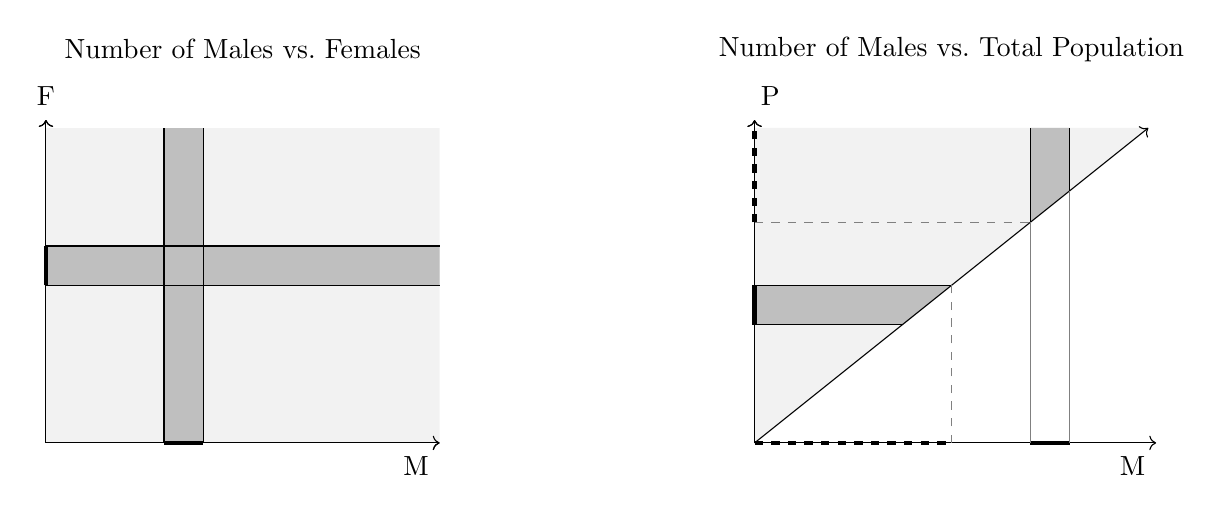
\begin{tikzpicture}
		\draw[->] (-1,3) -- (4,3);
		\draw[->] (-1,3) -- (-1,7.1);
		
		\node at (-1,7.4) {F};
		\node at (3.7,2.7) {M};
		
		\begin{scope}
			\clip (-1,3) rectangle (4,7);
			\fill[gray!10!white] (-1,3) rectangle (4,7);
		\end{scope}
		
		\begin{scope}
			\clip (-1,5) rectangle (4,5.5);
			\fill[gray!50!white] (-1,5) rectangle (4,5.5);
		\end{scope}
		
		\begin{scope}
			\clip (0.5,3) rectangle (1,7);
			\fill[gray!50!white] (0.5,3) rectangle (1,7);
		\end{scope}
		
		\begin{scope}
			\clip (0.5,5) rectangle (1,5.5);
			\fill[gray!50!white] (0.5,5) rectangle (1,5.5);
		\end{scope}
		
		\draw[black] (-1,5)--(4,5);
		\draw[black] (-1,5.5)--(4,5.5);
		
		\draw[black] (0.5,3) -- (0.5,7);
		\draw[black] (1,3) -- (1,7);
		
		
		\draw[->] (-1,3) -- (4,3);
		\draw[->] (-1,3) -- (-1,7.1);
		
		
		\draw[->] (8,3) -- (13.1,3);
		\draw[->] (8,3) -- (8,7.1);
		
		\draw[black,ultra thick] (-1,5) -- (-1,5.5);
		\draw[black,ultra thick] (0.5,3) -- (1,3);
		
		\node at (12.8,2.7) {M};
		\node at (8.2,7.4) {P};
		
		\begin{scope}
			\clip (8,3) -- (8,4.5) -- (9.89,4.5) -- (8,3);
			\fill[gray!10!white] (8,3) -- (8,4.5) -- (9.89,4.5) -- (8,3);
		\end{scope}
		\begin{scope}
			\clip (8,5) -- (10.5,5) -- (13,7) -- (8,7) -- (8,5);
			\fill[gray!10!white] (8,5) -- (10.5,5) -- (13,7) -- (8,7) -- (8,5);
		\end{scope}
		
		\begin{scope}
			\clip (8,4.5) -- (8,5) -- (10.5,5) -- (9.8,4.5) -- (8,4.5);
			\fill[gray!10!white] (8,4.5) -- (8,5) -- (10.5,5) -- (9.8,4.5) -- (8,4.5);
		\end{scope}
		
		\draw[->] (8,3) -- (8,7.1);
		
		
		\begin{scope}
			\clip (8,4.5) -- (8,5) -- (10.5,5) -- (9.89,4.5) -- (8,4.5);
			\fill[gray!50!white] (8,4.5) -- (8,5) -- (10.5,5) -- (9.89,4.5) -- (8,4.5);
		\end{scope}
		\begin{scope}
			\clip (11.5,5.8) -- (11.5,7) -- (12,7) -- (12,6.2) -- (11.5,5.8);
			\fill[gray!50!white] (11.5,5.8) -- (11.5,7) -- (12,7) -- (12,6.2) -- (11.5,5.8);
		\end{scope}
	
		\draw[->] (8,3) -- (13,7);
		
		\draw[black] (8,4.5) -- (9.89,4.5);
		\draw[black] (8,5) -- (10.5,5);	
		
		\draw[black, ultra thick, dashed] (8,3) -- (10.5,3);	
		\draw[black,ultra thick] (8,4.5) -- (8,5);
		
		\draw[gray,dashed] (10.5,3) -- (10.5,5);
		
		\draw[gray,dashed] (8,5.8) -- (11.5,5.8);
		
		\draw[black,ultra thick] (11.5,3) -- (12,3);
		\draw[black,ultra thick,dashed] (8,5.8) -- (8,7);
		
		\draw[gray] (11.5,3) -- (11.5,5.8);
		\draw[gray] (12,3) -- (12,6.2); 
		\draw[black] (11.5,5.8) -- (11.5,7);
		\draw[black] (12,6.2) -- (12,7);
		
		
		\node at (1.5,8) {Number of Males vs.~Females};
		\node at (10.5,8) { Number of Males vs.~Total Population};
\end{tikzpicture}
	\caption{Domain independence and projections. Given a population, the number of male and female members form independent domains: knowing something about one value tells us nothing about the other. Pictorially, a constraint on one side gives us a vertical or horizontal band, which projected on the other axis, gives us the full axis (i.e.~the certainty). On the other hand, the total population and the number of males are not independent domains: given the total population, the number of males cannot exceed that number; given the number of males, the total population cannot be lower than that number. Pictorially, we see that the combined domain does not span the whole plane. A constraint on one domain gives us, when projected, a constraint on the other domain.} \label{fig:2_relationships}
\end{figure}



\begin{mathSection}
	\begin{defn}
		The experimental domains of a countable set $\{\edomain_{X_i}\}_{i=1}^{\infty}$ are \textbf{independent} if taking one verifiable statement $\stmt_i \in \edomain_{X_i}$ from each domain always gives an independent set of statements.
	\end{defn}
	\begin{prop}
		Let $\{\edomain_{X_i}\}_{i=1}^{\infty}$ be a countable set of independent experimental domains and $X_i$ their respective possibilities. The set of possibilities $X$ of the combined experimental domain $\bigtimes\limits_{i=1}^{\infty} \edomain_{X_i}$ consists of all the possible conjunctions of the possibilities of each domain. That is: $X = \{ \bigAND\limits_{i=1}^{\infty} x_i \, | \, x_i \in X_i \}$. Notationally, we write $\edomain_X=\edomain_{\bigtimes\limits_{i=1}^{\infty} X_i}$.
	\end{prop}
	\begin{proof}
		A possibility $x \equiv \bigAND\limits_{i=1}^{\infty}x_i$ for the combined domain is the conjunction of possibilities of each individual domain by \ref{prop_combined_possibility}. Since the domains are independent and since possibilities are neither certainties nor impossibilities, by \ref{def_independent_statements} there exists an assignment $a \in \pAss$ such that $a(x_i) = \TRUE$ for all $i=1..\infty$ and therefore $a(x)=\TRUE$. That is, each conjunction $x=\bigAND\limits_{i=1}^{\infty}x_i$ is not impossible and therefore is a possibility.
	\end{proof}
	\begin{defn}
		Let $\{(X_i, \mathsf{T}_i)\}_{i=1}^{\infty}$ be a countable set of topological spaces. Let $X=\bigtimes\limits_{i=1}^{\infty} X_i$ be the Cartesian product of the points. Let $\mathcal{B}$ be the collection of sets of the form $\bigtimes\limits_{i=1}^{\infty} U_{i}$, with $U_i \in \mathsf{T}_i$ and $U_i \neq X_i$ only finitely many times. The topology generated by $\mathcal{B}$ is called the \textbf{product topology}.
	\end{defn}
	\begin{prop}
		Let $\{\edomain_{X_i}\}_{i=1}^{\infty}$ be a countable set of independent experimental domains. The natural topology for the possibilities of the combined experimental domain $\edomain_{\bigtimes\limits_{i=1}^{\infty} X_i}$ is the product topology of the natural topology for the possibilities of each domain.
	\end{prop}
	\begin{proof}
		Let $U_i : \edomain_{X_i} \to \mathsf{T}_{X_i}$ be the map from a verifiable statement of a domain to its verifiable set in the respective topology. Let $U : \edomain_{X} \to \mathsf{T}_X$ be the same map for the combined domain. Let $\stmt_i \in \edomain_{X_i}$ be a verifiable statement from a particular domain and $U_i(\stmt_i)$ its verifiable set in that domain. Since we also have $\stmt_i \in \edomain_{X}$, the statement is also associated with the verifiable set $U(\stmt_i)$ in the combined domain. Because the domains are independent, every possibility in $U_i(\stmt_i)$ is compatible with any possibility $x_j \in X_j$ for all $j \neq i$. This means that $U(\stmt_i)=X_1\times ... \times X_{i-1} \times U_i(\stmt_i) \times X_{i+1} \times ...$ . Given that a verifiable statement in the combined domain can be generated using finite conjunction and countable disjunction from the verifiable statements of the independent domains, the topology of the combined space can be generated by all sets of the form $\bigtimes\limits_{i=1}^{\infty} U_{i}$, with $U_i \in \mathsf{T}_i$ and $U_i \neq X_i$ only once. Using finite conjunction, this includes those sets where $U_i \neq X_i$ finitely many times. The natural topology of the combined domain is the product topology by definition.
	\end{proof}
\end{mathSection}

\subsection{Dependent domains}

Another special case is combining a domain $\edomain_X$ with another $\edomain_Y \subseteq \edomain_X$ that is dependent on it. For example, combining the domain for the temperature of a mercury column with the domain for its height. Since the height can be determined by the temperature, no new possibilities are added. The combined domain is equivalent to the independent domain $\edomain_X$ since all the verifiable statements in $\edomain_Y$ have equivalents in it.

\begin{mathSection}
	\begin{prop}
		Let $\edomain_X$ and $\edomain_Y$ be two experimental domains such that $\edomain_Y \subseteq \edomain_X$ depends on the first. Then $\edomain_X \times \edomain_Y \equiv \edomain_X$.
	\end{prop}
	\begin{proof}
		Since $\edomain_Y$ is dependent on $\edomain_X$, any statement in $\edomain_Y$ is equivalent to one in $\edomain_X$. Therefore no statement can be generated from them that is not equivalent to one already contained in $\edomain_X$. Therefore $\edomain_X \times \edomain_Y$ is equivalent to $\edomain_X$. 
	\end{proof}
	\begin{coro}
		Let $\edomain_X$ and $\edomain_Y$ be two experimental domains such that $\edomain_Y \subseteq \edomain_X$ depends on the first. The possibilities of $\edomain_X \times \edomain_Y$ are the possibilities of $\edomain_X$.
	\end{coro}
	\begin{proof}
		The possibilities of $\edomain_X \times \edomain_Y$ are the possibilities of $\edomain_X$ since they are equivalent domains. To be consistent with \ref{prop_combined_possibility}, we additionally show that they are also the subset of the scalar product. Let $f : X \to Y$ be the causal relationship between the domains, let $x$ and $y$ be two possibilities of the respective domains. We have $x \AND y \nequiv \impossibility$ if and only if $y = f(x)$, so the possibilities of $\edomain_X \times \edomain_Y$ are $x \AND f(x)$ for all $x \in X$. We also have $x \AND f(x) \equiv x$ since $x \narrower f(x)$.
	\end{proof}
\end{mathSection}


\subsection{Incompatible domains}

The last special case we consider is when the domains are incompatible, that is all verifiable statements of one are incompatible with the verifiable statements of the others. This is one case where the residual possibility behaves differently from all the others.\footnote{In fact, this is what prompted us to introduce the residual possibility.} Suppose $\edomain_X$ is the domain to classify a particular specimen as an animal and $\edomain_Y$ is the domain to classify it as a plant. If we take a verifiable statement from the first, such as \statement{that specimen has fur}, then it will be incompatible with a verifiable statement from the other, such as \statement{that specimen has lobed leaves}. The only way we can combine the possibilities is to take an established possibility of one (e.g. \statement{this specimen is a cat}) and combine it with the residual possibility of the other (e.g. \statement{this specimen is not a plant}). In other words, the combined possibilities are the union of the possibilities of the two domains (e.g. all possible plants and all possible animals).

In terms of the topology, the established possibilities of the combined domain are the disjoint union of the established possibilities of the original domains and their natural topology is the disjoint union topology (or co-product topology). 

\begin{mathSection}
	\begin{defn}
		Two experimental domains $\edomain_X$ and $\edomain_Y$ are \textbf{incompatible} if all verifiable statements in one are incompatible with all verifiable statements of the other. Formally, $\stmt_X \ncomp \stmt_Y$ for each pair of verifiable statements $\stmt_X \in \edomain_X$ and $\stmt_Y \in \edomain_Y$.
	\end{defn}
	\begin{coro}
		Let $\edomain_X$ and $\edomain_Y$ be two incompatible experimental domains. Then they must be incomplete and admit a residual possibility.
	\end{coro}
	\begin{proof}
		Let $\basis_X$ and $\basis_Y$ be a countable basis for the respective domain. Since we have $\stmt[e]_X \ncomp \stmt[e]_Y$ for all choices of $\stmt[e]_X \in \basis_X$ and $\stmt[e]_Y \in \basis_Y$, we also must have $\bigOR\limits_{\stmt[e]_X \in \basis_X} \stmt[e]_X \ncomp \bigOR\limits_{\stmt[e]_Y \in \basis_Y} \stmt[e]_Y$. Therefore $\bigOR\limits_{\stmt[e]_X \in \basis_X} \stmt[e]_X \nequiv \certainty$. Which means the residual possibility $\mathring{x} = \bigAND\limits_{\stmt[e]_X \in \basis_X} \NOT\stmt[e]_X = \NOT \bigOR\limits_{\stmt[e]_X \in \basis_X} \stmt[e]_X \nequiv \impossibility$. Therefore $\edomain_X$ is not complete and, by symmetry, neither is $\edomain_Y$.
	\end{proof}
	\begin{prop}
		Let $\{\edomain_{X_i}\}_{i=1}^{\infty}$ be a countable set of experimental domains pair-wise incompatible and $\dot{X}_i$ their respective established possibilities. The set of established possibilities $\dot{X}$ of the combined experimental domain $\bigtimes\limits_{i=1}^{\infty} \edomain_{X_i}$ consists of the disjoint union of the possibilities of each domain. That is: $\dot{X} = \coprod\limits_{i=1}^{\infty} \dot{X}_i = \bigcup\limits_{i=1}^{\infty} \dot{X}_i$ as $\dot{X}_i \cap \dot{X}_j = \emptyset$ for all $i,j \geq 1$ and $i \neq j$. Notationally, we write $\edomain_X=\edomain_{\coprod\limits_{i=1}^{\infty} X_i}$.
	\end{prop}
	\begin{proof}
		Consider two incompatible domains $\edomain_X$ and $\edomain_Y$. Let $\dot{x} \in X$ and $\dot{y} \in Y$ be two established possibilities. Then they both correspond to a minterm of the respective basis where at least one element is taken without negation. This also means that their conjunction will include the conjunction of one element of each of the basis. Since the elements of one basis are incompatible with the elements of the other, we have $\dot{x} \ncomp \dot{y}$.
		
		Now let $\dot{x} \in X$ be an established possibility, $\mathring{y} \in Y$ the residual and $\dot{Y} = Y \setminus \{\mathring{y}\}$ the established possibilities. We have $\dot{x} \equiv \dot{x} \AND \certainty \equiv \dot{x} \AND \bigOR\limits_{y \in Y} y \equiv \dot{x} \AND (\bigOR\limits_{\dot{y} \in \dot{Y}} \dot{y} \OR \mathring{y}) \equiv \bigOR\limits_{\dot{y} \in \dot{Y}} (\dot{x} \AND \dot{y}) \OR (\dot{x} \AND \mathring{y}) \equiv \impossibility \OR (\dot{x} \AND \mathring{y}) \equiv \dot{x} \AND \mathring{y}$. By symmetry, $\dot{y} \equiv \mathring{x} \AND \dot{y}$.
		
		To conclude, let $\mathring{x} \in X$ and $\mathring{y} \in Y$ be the two residual possibilities. The conjunction $\mathring{x} \AND \mathring{y}$ corresponds to a minterm where all the elements of the basis are negated. Therefore $\mathring{x} \AND \mathring{y}$ is the residual possibility of the combined domain, if it is not impossible. 
		
		Generalizing to a countable set of incompatible domains, the conjunction of all the residual possibilities $\mathring{x}= \bigAND_{i=1}^{\infty} \mathring{x}_i$ is the residual possibility of the combined domain, if it is not impossible. The only other conjunctions of the form $x= \bigAND_{i=1}^{\infty} x_i$ with $x_i \in X_i$ for all $i \geq 1$ that are not impossible are those where only one element is not a residual possibility. Those correspond to the established possibilities. But each of those conjunctions will be equivalent to the only element that is not a residual possibility. Therefore each established possibility of the combined domain is equivalent to an established possibility of one of the original domains: $\dot{X} = \bigcup\limits_{i=1}^{\infty} \dot{X}_i$. Given that the established possibilities of two incompatible domains are incompatible and therefore different, we have $\dot{X}_i \cap \dot{X}_j = \emptyset$ for all $i,j \geq 1$ and $i \neq j$. The established possibilities of the combined domains are the disjoint union of the established possibilities of the individual domains.
	\end{proof}

	\begin{defn}
		Let $\{(X_i, \mathsf{T}_i)\}_{i=1}^{\infty}$ be a countable set of topological spaces. Let $X=\coprod\limits_{i=1}^{\infty} X_i$ be the disjoint union of the points. The \textbf{disjoint union topology} $\mathsf{T}$ is the topology for which $U \in \mathsf{T}$ if and only if $U \cap X_i \in \mathsf{T}_i$ for all $i \geq 1$.
	\end{defn}

	\begin{prop}\label{prop_disjoint_union_topology_is_closure}
		The disjoint union topology is generated by closing the topologies of the initial spaces under disjoint union.
	\end{prop}
    \begin{proof}
		First we show that all disjoint unions of verifiable sets are part of the disjoint union topology. Let $\{(X_i, \mathsf{T}_i)\}_{i=1}^{\infty}$ be a countable set of topological spaces and $(X, \mathsf{T})$ their disjoint union with the disjoint union topology. Any disjoint union of verifiable sets can be put in the form $U=\coprod\limits_{i=1}^{\infty} U_i$ with $U_i \in \mathsf{T}_i$ for all $i \geq 1$. We have $U \cap X_i = \coprod\limits_{i=j}^{\infty} U_j \cap X_i = U_i$ for all $i \geq 1$. Therefore $U \in \mathsf{T}$ by definition.
		
		Now we show that any set in the disjoint union topology is the disjoint union of verifiable sets of the individual topologies. Let $U \in \mathsf{T}$. Since $U \subseteq X$ and $X$ is the disjoint union for all $X_i$, we can write $U=\coprod\limits_{i=1}^{\infty} U_i$. As before $U \cap X_i = U_i$ for all $i \geq 1$ and, since $U \cap X_i \in \mathsf{T}_i$ for all $i \geq 1$ by definition of the disjoint union topology, $U_i \in \mathsf{T}_i$ for all $i \geq 1$. Therefore any $U \in \mathsf{T}$ is the disjoint union of verifiable sets.
		
		This also shows that the disjoint union topology is a topology since it is closed under arbitrary union by definition, it is closed under finite intersection within each topology and it is closed under finite intersection across topologies since their intersection is always the empty set.
    \end{proof}

	\begin{prop}
		Let $\{\edomain_{X_i}\}_{i=1}^{\infty}$ be a countable set of pair-wise incompatible domains. The natural topology for the established possibilities of the combined experimental domain $\edomain_{\coprod\limits_{i=1}^{\infty} X_i}$ is the disjoint union topology of the natural topology for the established possibilities of each domain.
	\end{prop}
	\begin{proof}
		Given that the domains are incompatible, they are also incomplete. The only statement in each domain $\edomain_{X_i}$ compatible with the respective residual possibility $\mathring{x}_i$ will be the certainty $\certainty$. This means the natural topology restricted to the established possibilities contains all the verifiable sets associated to the impossibilities and to all verifiable statements. This will also be true for the combined domain $\edomain_{\coprod\limits_{i=1}^{\infty} X_i}$, if it is incomplete. If it is complete, then the established possibilities are the full possibilities and their natural topology coincides. Note that all verifiable statements in the combined domain can be generated from the verifiable statements of the individual domains. Also note that the conjunction between the different domains is an impossibility and therefore does not yield a new statement. Therefore all the statements whose verifiable sets form the topology on the established possibilities on the combined domain can be generated by the disjunction of all the statements whose verifiable sets form  the topology on the established possibilities on the individual domains. Therefore the topology of the combined space is simply closing the individual topologies under the disjoint union. The topology of the combined space is therefore the disjoint union topology by \ref{prop_disjoint_union_topology_is_closure}
	\end{proof}
\end{mathSection}

For topologies, as well as for other mathematical structures, we can choose between two types of products. If we have two one dimensional euclidean spaces we can decide whether to take their product (i.e. the plane) or their co-product (i.e. the disjoint union of the two lines). For experimental domains we do not choose: it is what it is. There is no way to combine the two experimental domains for temperature and height of the same mercury column and get the Cartesian product of their possibilities. Though combining two independent domains mimics the categorical product and combining two incompatible domains mimics the categorical co-product, it is the semantic (and ultimately physical) relationship between them that decides which product we have. This is another case where the mathematical structures ``forget" the full equivalence. The topology only captures how the temperature and height can be measured, and not whether they are independent, dependent or incompatible. That information lies outside of the topology and therefore needs to be added by choosing the correct combination.

\section{Experimental domain for experimental relationships}

Now that we have seen how to describe relationships between domains, we should ask: are experimental relationships themselves something we can experimentally verify? We may know that there is a relationship between the temperature of a mercury column and its height, but how can we confirm experimentally which one it is?

The main result of this section is to show that, given two related experimental domains, we can always mathematically construct from them another experimental domain for which the possibilities are continuous functions between the possibilities of the original domains. This means that, since we can recursively create relationship domains about relationship domains, the universe of discourse of our mathematical framework is closed. Yet, the availability of the experimental tests (i.e. whether the statements we construct are actually verifiable) is not guaranteed.

First of all we have to clarify within our framework what it means to experimentally verify a relationship. Suppose $\edomain_X$ is the domain for the state of a light switch, up or down being the two possibilities, and $\edomain_Y$ is the domain for the state of the light, which can be on or off. Suppose we could have three cases: the one where the switch is wired correctly, up corresponding to on, the one where the switch is wired incorrectly, up corresponding to off, and the one where the switch is not actually wired to the light, the two domains are independent. Each of these cases is represented by a different set of logical relationships, a different set of possible assignments.

\begin{table}[h]
\centering
\begin{tabular}{c|c|c|c}
\multicolumn{2}{c|}{X} & \multicolumn{2}{c}{Y} \\
	up & down & on & off \\
	\hline
	T & F & T & F \\
	F & T & F & T \\
\end{tabular}
\caption{Case 1: switch wired correctly to the light}
\end{table}

\begin{table}[h]
\centering
\begin{tabular}{c|c|c|c}
	\multicolumn{2}{c|}{X} & \multicolumn{2}{c}{Y} \\
	up & down & on & off \\
	\hline
	T & F & F & T \\
	F & T & T & F \\
\end{tabular}
\caption{Case 2: switch wired incorrectly to the light}
\end{table}

\begin{table}[h]
	\centering
	\begin{tabular}{c|c|c|c}
		\multicolumn{2}{c|}{X} & \multicolumn{2}{c}{Y} \\
		up & down & on & off \\
		\hline
		T & F & T & F \\
		T & F & F & T \\
		F & T & T & F \\
		F & T & F & T \\
	\end{tabular}
	\caption{Case 3: switch not wired to the light}
\end{table}

Each case, then, is a different model: a different logical context. To experimentally verify which model is the right one means verifying statements of the type \statement{it is possible for the switch to be up while the light is on}. This does not correspond to \statement{the switch is up} $\AND$ \statement{the light is on} but to \statement{the switch is up} $\comp$ \statement{the light is on}. These are statements about the table and they cannot be columns of the table itself. What we need to create is a metacontext, in which each line corresponds to one choice of model, to one context.

\begin{table}[h]
	\centering
	\begin{tabular}{r|c|c|c|c}
		& up $\comp$ on & down $\comp$ on & up $\comp$ off & down $\comp$ off \\
		\hline
		Case 1 & T & F & F & T \\
		Case 2 & F & T & T & F \\
		Case 3 & T & T & T & T \\
	\end{tabular}
	\caption{Possible assignments for the metacontext}
\end{table}

Each line will tell us what statements are compatible and given the truth values of the line we can reconstruct the model. The verifiable statements that distinguish between different models, therefore, live in this metacontext and so will the experimental domain for the relationships.

\begin{mathSection}
	\begin{defn}
		Let $\logCtx_1$ and $\logCtx_2$ be two logical contexts. Let $S_1 \subseteq \logCtx_1$ and $S_2 \subseteq \logCtx_2$ be sets of statements. We say $f : S_1 \to S_2$ is a \textbf{logic homomorphism} if it preserves the logical structure. That is:
		\begin{itemize}
			\item possible assignments on $S_2$ correspond to possible assignments on $S_1$: if $a_2 \in \pAss[S_2]$ then there exists $a_1 \in \pAss[S_1]$ such that $a_1(\stmt) = a_2(f(\stmt))$ for all $\stmt \in S_1$
			\item a verifiable statement of $S_1$ is mapped to a verifiable statement in $S_2$
		\end{itemize}
		Additionally, if there exists a logic homomorphism $g : S_2 \to S_1$ such that $f \circ g = \Id_{S_1}$ and $g \circ f = \Id_{S_2}$ then $f$ is a \textbf{logic isomorphism} and $g$ is the \textbf{inverse} of $f$. Two logic isomorphisms $f : S_1 \to S_2$ and $g : S_1 \to S_2$ are equivalent if $f(\stmt)\equiv g(\stmt)$ for all $\stmt \in S_1$.
	\end{defn}

\begin{coro}\label{3_coro_logic_homomorphism_preserves_boolean}
	Let $h : S_1 \to S_2$ be a logic homomorphism, then for every $\hat{\stmt} \in S_1$, $\hat{S} \subseteq S_1$ and $f_\Bool : \Bool^{\hat{S}} \to \Bool$ such that $a_1(\hat{\stmt}) = f_\Bool(\{ a_1(\stmt) \}_{\stmt \in \hat{S}})$ for all $a_1 \in \pAss[S_1]$, then $a_2(h(\hat{\stmt})) = f_\Bool(\{ a_2(h(\stmt)) \}_{\stmt \in \hat{S}})$ for all $a_2 \in \pAss[S_2]$. In particular:
	\begin{itemize}
		\item $h(\NOT \stmt) \equiv \NOT h(\stmt)$ for all $\stmt \in S_1$
		\item $h(\bigAND_{\stmt \in S} \stmt) \equiv \bigAND_{\stmt \in S} h(\stmt)$ for all $S \subseteq S_1$
		\item $h(\bigOR_{\stmt \in S} \stmt) \equiv \bigOR_{\stmt \in S} h(\stmt)$ for all $S \subseteq S_1$
	\end{itemize}
\end{coro}

\begin{proof}
	If $a_1(\hat{\stmt}) = f_\Bool(\{ a_1(\stmt) \}_{\stmt \in \hat{S}})$ for all $a_1 \in \pAss[S_1]$ then, by the first property of logic homomorphisms, there is no $a_2 \in \pAss[S_2]$ such that $a_2(h(\hat{\stmt})) \neq f_\Bool(\{ a_2(h(\stmt)) \}_{\stmt \in \hat{S}})$. Therefore $a_2(h(\hat{\stmt})) = f_\Bool(\{ a_2(h(\stmt)) \}_{\stmt \in \hat{S}})$ for all $a_2 \in \pAss[S_2]$.
	
	In particular, since the relationship holds for any arbitrary $f_\Bool$, it will hold for negation, arbitrary conjunction and arbitrary disjunction.
\end{proof}

\begin{prop}
	Let $\logCtx_1$ and $\logCtx_2$ be two logical contexts. Let $S_1 \subseteq \logCtx_1$ and $S_2 \subseteq \logCtx_2$ be sets of statements and $f : S_1 \to S_2$ a logic homomorphism. Let $\bar{S}_1 \subseteq \logCtx_1$ and $\bar{S}_2 \subseteq \logCtx_2$ be the closure of $S_1$ and $S_2$ respectively under arbitrary conjunction, arbitrary disjunction and negation. Then if there exists a logic homomorphism $\bar{f} : \bar{S}_1 \to \bar{S}_2$ such that $\bar{f}(\stmt_1) \equiv f(\stmt_1)$ for all $\stmt_1 \in S_1$ it is unique.
\end{prop}

\begin{proof}
	Let $\tstmt_1 \in \bar{S}_1$ but $\tstmt_1 \notin S_1$. Then $\tstmt_1$ depends on $S_1$ through some $g_\Bool : \Bool^{S_1} \to \Bool$. Let $\bar{f}_1 : \bar{S}_1 \to \bar{S}_2$ and $\bar{f}_2 : \bar{S}_1 \to \bar{S}_2$ be two logic homomorphisms such that $\bar{f}_1(\stmt_1) \equiv \bar{f}_2(\stmt_1) \equiv f(\stmt_1)$ for all $\stmt_1 \in S_1$. Then by \ref{3_coro_logic_homomorphism_preserves_boolean} both $\bar{f}_1(\tstmt_1)$ and $\bar{f}_2(\tstmt_1)$ depend on $S_2$ through $g_\Bool$. This means that in every possible assignment $a \in \pAss[\bar{S}_2]$ we have $a(\bar{f}_1(\tstmt_1)) = a(\bar{f}_2(\tstmt_1))$  and therefore $\bar{f}_1(\tstmt_1) \equiv \bar{f}_2(\tstmt_1)$. Then $\bar{f}_1$ and $\bar{f}_2$ are equivalent.
\end{proof}


\begin{defn}
	Let $\edomain_X, \edomain_Y \subseteq \logCtx$ be two experimental domains. The \textbf{relationship metacontext}  $\logCtx_{C(X,Y)}$ between $\edomain_X$ and $\edomain_Y$ over $\{ \logCtx_i \}_{i \in I}$ is defined by following construction. Let $I$ be an index set. Let $\{ \logCtx_i \}_{i \in I}$ be an indexed set of logical contexts, let $\{ \edomain_{X_i} \}_{i \in I}$ and $\{ \edomain_{Y_i} \}_{i \in I}$ be two indexed sets of experimental domains such that $\edomain_{X_i}, \edomain_{Y_i} \subseteq \logCtx_i$ for all $i \in I$. Let $\{f_{i}\}_{i \in I}$ be a set of logic isomorphisms such that $f_{i} : \edomain_{X} \to \edomain_{X_i}$. Let $\{g_{i}\}_{i \in I}$ be a set of logic isomorphisms such that $g_{i} : \edomain_{Y} \to \edomain_{Y_i}$.
	
	Let $S$ be the set of ordered pairs of $\edomain_{X}$ and $\edomain_{Y}$ and \statement{$\stmt_x \comp \stmt_y$} be the notation of an element of $S$ for some $\stmt_x \in \edomain_{X}$ and $\stmt_y \in \edomain_{Y}$. For each $i \in I$, let $a_i \in \Bool^S$ be such that  $a_i(``\stmt_x \comp \stmt_y") = \TRUE$ if and only if $f_{i}(\stmt_x) \comp g_{i}(\stmt_y)$. Define $\pAss = \{ a_i \, | \, \forall i \in I \}$. Assume $a_i \neq a_j$ if $i \neq j$; if not, given a subset of $I$ that leads to the same possible assignment, remove all elements but one. Pick $t \in I$ and define $\truth = a_t$.
	
	Given an arbitrary function $f_\Bool : \Bool^S \to \Bool$, we can extend the set $S$ with a new element for which the possible assignments are calculated according to the function. The relationship context $\logCtx_{C(X,Y)}$ is the closure of $S$ under all possible functions $f_\Bool \in \Bool^S$.
	
	Let $S_v \subseteq S$ be set of statements \statement{$\stmt_x \narrower \stmt_y$}=\statement{$\stmt_x \ncomp \NOT \stmt_y$}=$\NOT$\statement{$\stmt_x \comp \NOT \stmt_y$} such that $\stmt_x \in \edomain_{X}$ and $\stmt_y \in \edomain_{Y}$ are verifiable. The set of verifiable statements $\vstmtSet \subseteq \logCtx$ for the relationship context is the set of statements generated by $S_v$ using finite conjunction and countable disjunctions.
\end{defn}
\begin{justification}
	By constructions, the relationship context satisfies the axioms for a logical context. We have a set of elements and a set of possible assignments of which one is the truth, this satisfies axioms \ref{ax_statement} and \ref{ax_possible_assignemetns}. Some of the statements are verifiable and satisfy \ref{ax_verifiable_statements}. Closure for axioms \ref{ax_functions_of_statement}, \ref{ax_verifiable_AND} and \ref{ax_verifiable_OR} are satisfied by constructions. We need to clarify why and what cases this construct makes physical sense.
	
	The set $\{ \logCtx_i \}_{i \in I}$ consists of different contexts, each containing a copy of the domains $\edomain_X$ and $\edomain_Y$ with a different relationship between them. For example, if $\edomain_X$ is the domain for a light switch, up or down being the possibilities, and $\edomain_Y$ is the domain for the light, being on or off, in one context the two domain may have a causal relationship (i.e. the switch is wired to the light), in another they may have a different causal relationship (i.e. the switch is wired in the wrong way), and in yet another they may be independent (i.e. switch is not wired with the light). The logic isomorphisms $\{f_{i}\}_{i \in I}$ and $\{g_{i}\}_{i \in I}$ allow us relate the statements that represent the same  assertion in the different contexts.
	
	Note that while mathematically we can always construct the relationship metacontext, it may not exist in reality. Specifically, there is nothing that guarantees that statements of the form \statement{$\stmt_x \narrower \stmt_y$} are actually verifiable.
\end{justification}
\end{mathSection}

Now that we have the right context, we have to understand what is the right basis to generate the experimental domain. Suppose we have a way to verify experimentally statements of the type \statement{the temperature of the mercury column is between 24 and 25 Celsius}$\narrower$\statement{the height of the mercury column is between 24 and 25 millimeters}. That is, we can verify that whenever $\stmt_X=$\statement{the temperature of the mercury column is between 24 and 25 Celsius} is verified, then $\stmt_Y=$\statement{the height of the mercury column is between 24 and 25 millimeters} is verified. In that case, we can explore the connection between the two domains within different ranges at ever increasing precision. This means we can narrow the range of possible functions in the same way that we can narrow the range of possible values for a quantity. These types of statements, then, form an experimental domain where each possibility corresponds to a possible continuous function between the two initial experimental domains.

\begin{mathSection}
	\begin{defn}
		Let $\logCtx_{C(X,Y)}$ be the relationship metacontext between $\edomain_X$ and $\edomain_Y$ over $\{ \logCtx_i \}_{i \in I}$. Let $\edomain_{Y_i} \subseteq \edomain_{X_i}$ for all $i \in I$. Let $\basis_X \subseteq \edomain_X$,  $\basis_Y \subseteq \edomain_Y$ be the two countable basis of the respective domains and let $\basis = \{ ``\stmt[e]_x \narrower \stmt[e]_y" \, | \,  \stmt[e]_x \in \basis_X, \stmt[e]_y \in \basis_Y\}$. Then the \textbf{relationship domain} $\edomain_{C(X,Y)}$ is the experimental domain generated by $\basis$.
	\end{defn}
	\begin{proof}
		The only thing that needs to be checked is that the basis that generates $\edomain_{C(X,Y)}$ is countable. Since $\basis_X$ and $\basis_Y$ are countable, the set of statements of the form $\mathbin{\narrower}(\stmt[e]_x, \stmt[e]_y)$ with $\stmt[e]_x \in \basis_X$ and $ \stmt[e]_y \in \basis_Y$ is also countable.
	\end{proof}
\begin{prop}\label{2_prop_relationship_domain_is_space_of_continuous_functions}
	The possibilities for a relationship domain $\edomain_{C(X,Y)}$ coincide with the possible experimental relationships between $X$ and $Y$. That is, for each possibility $z$ of $\edomain_{C(X,Y)}$ there exists a continuous function $f_z : X \to Y$ such that $z\equiv\bigAND\limits_{x\in X} ``x \narrower f_z(x)"$ and an $i \in I$ such that $\bar{g}_i(f_z(\bar{f}_i^{-1}(x_i))) \equiv f_c (x_i)$ for all $x_i \in X_i$ where $f_c$ is the causal relationship between $\edomain_{X_i}$ and $\edomain_{Y_i}$.
\end{prop}
\begin{proof}
	First we show that for each possibility $z$ of the relationship domain there exists a set $P_z \subseteq X \times Y$ such that $z \equiv \bigAND\limits_{(x,y) \in P_z} ``x \comp y"  \AND \bigAND\limits_{(x,y) \nin P_z} ``x \ncomp y"$. Let $z$ be a possibility of a relationship domain. This will be a minterm of the basis therefore $z \equiv minterm(\basis)$. Let $x \in X$ and $y \in Y$ be two possibilities and consider the statement $``x \comp y"$. If $z$ is true in a possible assignment, then the truth value for all statements of the form $``e_x \narrower e_y"$ where $(e_x, e_y) \in \basis_X \times \basis_Y$ will be set. But $x \ncomp y$ if and only if there exists at least one pair $(e_x, e_y) \in \basis_X \times \basis_Y$ such that $x \narrower e_x \narrower e_y$ and $y \ncomp e_y$. Therefore if $z$ is true in an assignment it will tell us whether $x \ncomp y$ is true or not, so we either have $z \narrower ``x \comp y"$ or $z \narrower \NOT ``x \comp y"$. Let $P_z = \{ (x,y) \in X \times Y \, | \, z \narrower ``x \comp y" \}$ and $\hat{z} = \bigAND\limits_{(x,y) \in P_z} ``x \comp y" \AND  \bigAND\limits_{(x,y) \nin P_z} \NOT ``x \comp y" $. Then $z \narrower \hat{z}$.
	
	Conversely, if we suppose $\hat{z}$ to be true in an assignment, then we will know the truth assignment for all statements of the form $``x \comp y"$ where $(x,y) \in X \times Y$. Let $(e_x, e_y) \in \basis_X \times \basis_Y$ and consider the statement $``e_x \narrower e_y"$. We have $e_x \narrower e_y$ if and only if there is no pair $(x,y)$ such that $x \narrower e_x$, $y \ncomp e_y$ and $x \comp y$. Therefore if $\hat{z}$ is true in an assignment it will tell us whether $e_x \narrower e_y$ is true or not, so we either have $\hat{z} \narrower ``e_x \narrower e_y"$ or $\hat{z} \narrower \NOT ``e_x \narrower e_y"$. As $z$ is a minterm of statements of the form $``e_x \narrower e_y"$, we'll either have $\hat{z} \narrower z$ or $\hat{z} \ncomp z$. Since $z \narrower \hat{z}$,  $\hat{z} \comp z$ and therefore $\hat{z} \narrower z$. Since we also have $z \narrower \hat{z}$, then we have $z \equiv \hat{z}$.
	
	Now we want to show that for each possibility $z$ there is a function $f_z : X \to Y$ such that $z\equiv\bigAND\limits_{x\in X} ``x \narrower f_z(x)"$. We note that statements of the form $``\stmt_x \comp \stmt_y$ are precisely the statements used to generate the relationship metacontext. Statements of the form $``x \comp y"$, where $x \in X$ and $y \in Y$, are enough to determine the truth value of statements of the form $``\stmt_x \comp \stmt_y$. Therefore for each possibility $z$ there is be one and only one possible truth assignment in which $z$ is true. That is, each $x$ correspond to particular logical context $\logCtx_i$. Since in that context $\edomain_{Y_i} \subseteq \edomain_{X_i}$ there will be a causal relationship $f_i : X_i \to Y_i$ such that $x_i \narrower f_i (x_i)$ which means $x_i \comp y_i$ if and only if $y_i = f_i(x_i)$. Since causal relationships are unique and the possible assignments are distinct, to each $z$ will correspond a unique $f_z : X \to Y$ such that $\bar{g}_i \circ f_z \circ \bar{f}^{-1}_i = f_i$ and $z\equiv\bigAND\limits_{x\in X} ``x \narrower f_z(x)"$. Moreover $f_z$ is continuous since $\bar{f}_i$ and $\bar{g}_i$ are logical isomorphisms.
\end{proof}
\end{mathSection}

Note that the definition for the metacontext simply declares some statements to be verifiable: it does not guarantee that this is actually possible. So when can we do it? Or better, what do we need in practice to be able to build the necessary confidence? Let's think how we would test the relationship between temperature and height of a mercury column. We would prepare different mercury samples with different values of temperatures in many different conditions, measure height and temperature with different devices, repeat many times, ask someone else to do it independently, compare results, and so on. At some point we will have explored enough of the possible cases, checked and tried anything that could invalidate the result and we will have the confidence to say that \statement{if the temperature of the mercury column is between 24 and 25 Celsius then its height is between 24 and 25 millimeters}. We should stress that the procedure is not at all to observe a few values and then generalize. It is not mere induction. It is the ability to prepare and control the system in many different conditions and our inability to violate the relationship that gives us the confidence needed to reach the conclusion.

Suppose, in fact, that we want to experimentally verify the link between inflation and money supply. As long as we cannot create new countries in different economic conditions, the only thing we can do is gather data for as many nations as we can throughout history.\footnote{Computer simulations can sometimes alleviate this problem, though they are only as good as the model one uses.} Since we cannot purposely explore different conditions and we can't even replicate older ones, the best we can do is show that there was a correlation between those specific values. It is the inability to freely and fully explore the problem space that may not enable us to experimentally verify the causal relationship.\footnote{In this sense, experimental sciences allow for more rigorous results than observational sciences precisely because it is more feasible to experimentally test relationships between domains.}

The point is that we cannot give a general purpose algorithm for how to construct experimental tests for the relationships starting from the experimental tests of the individual domains. We cannot formalize in general what it means that we have explored the space ``enough" to consider the relationship verified, no more than we can formalize when the data collected is ``enough" to consider a statement verified or when a statement is specific ``enough" to consider the semantics well defined. This is where the practice of experimental science comes in.

But, while we may not know in general whether we can experimentally verify a relationship between two specific domains, we do know that the relationship domain can always be constructed in principle and therefore our mathematical framework is complete. That is: we can take two experimental domains (e.g. $\edomain_t$ for time and $\edomain_x$ for position), construct a relationship domain between them (e.g. $\edomain_{x(t)}$ for trajectories in space), then take another experimental domain (e.g. $\edomain_{(q,p)}$ for the states) and construct another relationship domain between the two (e.g. $\edomain_{(q,p)\to x(t)}$ for the relationship between states and trajectories). Our general mathematical theory of experimental science is therefore closed, since we can recursively create relationship domains about relationship domains indefinitely while remaining within its bounds. In other words, experimentally distinguishable objects and their relationships will never lie outside of the theory.


\section{Summary}

In this chapter we have seen the first important set of consequences of our general mathematical theory of experimental science. We have seen that experimental relationships between domains can be defined in terms of inference between verifiable statements or equivalently in terms of causal relationship between possibilities. The causal relationship always corresponds to a continuous function in the natural topology. Moreover, it will need to preserve any additional mathematical structure that formalizes a physical characteristic of the domain.

We have also seen how to combine a set of countably many experimental domains and how the combined possibilities depend on the logical and semantic relationships that exist across domains. Depending on the case, we can have the scalar product of the possibilities (with the product topology) all the way to the disjoint union of the established possibilities (with the disjoint union topology).

We have shown that it is possible to construct experimental domains for the relationships themselves. This means that within our theory we can describe relationships of arbitrarily higher order (i.e. relationships about relationships) and therefore we never go outside of our framework.

As we have only explored simple constructions based on the original concepts, these conclusions are of a general nature and therefore must apply to any area of science. 

\chapter{Properties and quantities}

In this chapter we will introduce the idea of \textbf{properties}, which we use to label the possibilities of an experimental domain. For example, we may use names to distinguish among people, fur color to distinguish among cats, pressure to distinguish the state of a gas. In particular, we'll define a \textbf{quantity} as a property that has a magnitude: we can compare two different values and determine which one is greater or smaller.

Instead of simply assuming we have quantities, we will need to construct them from the verifiable statements of an experimental domain. To do that, we will prove three theorems that will give necessary and sufficient conditions for that construction, clarifying how quantities are defined experimentally. These theorems will allow us to understand how the ordering of the values for a quantity are linked to the logical relationships between the verifiable statements, and in particular how the ordering of values is linked to the ordering defined by narrowness.

After characterizing quantities in general, we will see the cases of \textbf{discrete} and \textbf{continuous} quantities. We will see how discrete quantities are linked to decidability, the ability to verify both a statement and its negation, while continuous quantities are linked to a lack thereof. We will then discuss how the requirements for continuous quantities cannot be truly realized in practice and what happens when that idealization fails.

\section{Properties}

Whether the result of direct observation or not, a physical object is most often identified by its properties and their values. A person may be identified by name and date of birth; a bird may be characterized by the color of its beak; the state of a particle may be qualified by its position and momentum.

In this section we define how in general we can use properties to label the possibilities of an experimental domain. Each property will specify a continuous function from the possibilities to the topological space of the possible property values. Some properties may fully identify each possibility, as they assign distinct values, and some may also fully characterize which statements are verifiable.

Suppose $\edomain_X$ is a domain for animal identification and $X$, its possibilities, are all animal species. Providing good names and definitions for species is a whole scientific subject by itself (i.e. taxonomy) with its own rules (i.e. the International Code of Zoological Nomenclature). The ICZN assigns each species a name composed of two Latin words. For example, \statement{Passer domesticus} is the official name for the house sparrow while \statement{Passer italiae} is the one for the Italian sparrow. This means that identifying an animal species is equivalent to identifying its name. Therefore the domain to identify the species name $\edomain_{\mathcal{Q}} \equiv \edomain_X$ is equivalent to the one for identifying the actual species and we have an experimental relationship $q: X \to \mathcal{Q}$ between them. As each species is given a unique name this is the most discriminating type of property: one that covers the whole range of possibilities and fully identifies each of them. But this is a special case.

The ICZN also assigns a genus (pl. genera) to each species, which corresponds to the first part of the species name. For example, both aforementioned sparrows are of the genus \statement{Passer} while all swans, black or white, are of the genus \statement{Cygnus}. Now suppose that $\mathcal{Q}$ is the set of all names for all genera and $q: X \to \mathcal{Q}$ is the function that gives us the genus name for each species. We can still use this as a label for our possibilities, but it does not fully identify them.

On a different note, we could decide to distinguish species by their morphological attributes. For example, if $\mathcal{Q}$ is the set of all colors, we can imagine a function that gives us the beak color for each species. The function is partial, not defined on all elements, as not all species have a beak or its color may not be unique. We have $q: U \to \mathcal{Q}$ where $U \subseteq X$ is the set where the property is defined. To be consistent, though, we must at least be able to tell in what cases the property is actually defined. For example, we must be able to tell whether an animal has a beak. Therefore there must be a verifiable statement that is true if and only if the property is well defined. The set $U$, then, must correspond to the verifiable set of said statement.

Other examples of properties include: postal addresses for buildings, tax ID numbers for people, generation for fundamental particles, position of the center of mass of a body. In all these cases, the general pattern is that we assign a label to a possibility from an established set.

\begin{mathSection}
	\begin{defn}
		A \textbf{property} for an experimental domain $\edomain_X$ is any attribute we can use to distinguish between its possibilities. Formally, it is a tuple $(\mathcal{Q}, q)$ where $\mathcal{Q}$ is a topological space and $q : U \to \mathcal{Q}$ is a continuous function where $U \in \mathsf{T}_X$ is a verifiable set of possibilities.
	\end{defn}
	\begin{justification}
		Suppose $q$ is a physical property that can be assigned to distinguish the set of possibilities $U \subseteq X$. We must be able to tell experimentally whether the property is defined for each possibility. Therefore we are justified to assume that $U$ is a verifiable set. Let $\mathcal{Q}$ be the set of possible values for the property. Each element $U$ will be matched with a possible value. Therefore we are justified to assume there is a function $q : X \to \mathcal{Q}$ that specifies that mapping.
		
		As we must be able to experimentally distinguish between the values in $\mathcal{Q}$, there must be a collection $\mathsf{T}_Q$ of verifiable sets that corresponds to the possible verifiable statements associated to the quantity. Therefore we are justified to assume $\mathcal{Q}$ is a topological space. Moreover, since the property value is determined by each possibility, the function $q$ establishes a causal relationship between the two and therefore we are justified to assume $q$ is a continuous function.
	\end{justification}
\end{mathSection}
		
Note that we have not defined a property as an experimental domain. The possibility of the domain for a property would be a statement like \statement{the species name for this animal is Passer domesticus} while the value is just the object \statement{Passer domesticus}. The idea is that the property and its values are defined independently of the particular object. For example, distance in meters is defined independently of whether we later want to measure the earth diameter or its distance to the moon.\footnote{While in principle we could envision a formal construction of properties and their values purely built on top of the notion of statement (e.g. define the value \emph{red} to be the set of all statements that claim that something is of that color) we are not going to do so. While appealing in some respects, it is not clear whether such a construction would actually help to clarify underlying assumptions while it is clear it would distract from other more critical issues.}

The fact that the property and its values are defined more generally leads to some subtle issues: even if each possibility of the domain corresponds to one property value and each verifiable statement of the property is equivalent to a verifiable statement of the domain, the reverse may not be true. Consider the experimental domain for identifying negatively charged fundamental particles. In this case, each particle will correspond to a unique value of mass, and by measuring the mass we can infer the particle. But for each possible value of mass we will not have a possible fundamental particle. Moreover, the verifiable statement \statement{this particle is an electron} would correspond to an infinitely precise statement of the form \statement{the mass of the particle is exactly 510998.9461... eV} which is not verifiable. The reason is that identifying a negatively charged particle is not the same as measuring its mass with arbitrary precision: in the first case we can stop when there is only one possible particle within the finite range of our measurement. Now consider the experimental domain for the position of the center of mass of a particle along a particular direction. Not only is the distance from a fixed point enough to identify the position, but for each value of the distance we also have a possible position of the particle.

We say that a property fully characterizes an experimental domain if each possible value of a property corresponds to a possibility of the domain, like in the case of the distance from a reference and position of a particle. The idea is that it tells us what cases are possible and how they are experimentally verified. Instead, we say that a property fully identifies an experimental domain if each possibility corresponds to a unique value, like in the case of the mass of a negatively charged particle. The idea is that the value of the property allows us to uniquely identify the possibility but nothing more.

\begin{mathSection}
	\begin{defn}
		The possibilities of an experimental domain are \textbf{fully identified} by a property if its value is enough to uniquely determine a possibility. Formally, let $(\mathcal{Q}, q)$ be a property for an experimental domain $\edomain_X$. Then the possibilities $X$ are fully identified if $q: X \to \mathcal{Q}$ is injective.
	\end{defn}
	
	\begin{defn}
		An experimental domain is \textbf{fully characterized} by a property if all verifiable statements in the domain correspond to verifiable statements on the property and vice-versa. Formally, let $(\mathcal{Q}, q)$ be a property for an experimental domain $\edomain_X$. Then it is fully characterized if $q: X \to \mathcal{Q}$ is a homeomorphism.
	\end{defn}
\end{mathSection}

\section{Quantities and ordering}

We now focus our attention on those properties that can be quantified. The number of people in a group can be quantified by an integer, the distance between two objects can be quantified in meters, the force acting on a body can be quantified by the magnitude of a vector expressed in Newtons. The defining characteristic for a quantity is that a value can be greater, smaller or equal to another.

In this section we will define a quantity as a property with a linear order which we assume given a priori, and study its relationship with the experimental domain. We will define the order topology, which assumes one can experimentally verify whether a value is before or after another one. We will see that a domain is fully characterized by a quantity only if the possibilities themselves can be ordered, and how this ordering, in the end, is uniquely characterized by statement narrowness: 10 is less than 42 because \statement{the quantity is less than 10} is narrower than \statement{the quantity is less than 42}.

As the defining characteristic for a quantity is the ability to compare its values, then the values must be ordered in some fashion from smaller to greater. Therefore, given two different values, one must be before the other. Mathematically, we call linear order an order with such a characteristic as we can imagine the elements positioned along a line. Note that vectors are not linearly ordered: no direction is greater than the other. Therefore, in this context, a vector will not strictly be a quantity but a collection of quantities.\footnote{In other languages, there are two words to differentiate quantity as in ``physical quantity" (e.g. grandezza, Gr\"osse, grandeur) and as in ``amount" (e.g. quantit\`a, Menge, quantit\'e). It is the second meaning of quantity that is captured here.}

We also have to define how this order can be experimentally verified. The idea is that we should, at least, be able to verify that the value of a given quantity is before or after a set value. This allows us to construct bounds such as \statement{the mass of the electron is $511 \pm 0.5$ keV} which we take to be equivalent to \statement{the mass of the electron is more than 510.5 keV but less than 511.5 keV}.\footnote{The sentence \statement{the mass of the electron is $511 \pm 0.5$ keV} could instead be referring to statistical uncertainty instead of an accuracy bound and would constitute a different statement when the different meaning is attached. We will be treating these types of statistical statements later in the book, but suffice it to say that they cannot be defined before statements that identify bounds.} For integers, this also allows us to verify particular numbers as \statement{the earth has one natural satellite} is equivalent to the \statement{the earth has more than zero natural satellites and fewer than two}. Therefore we will define the order topology as the one generated by sets of the type $(a, \infty)$ and $(-\infty, b)$.

A quantity, then, is an ordered property with the order topology.

\begin{mathSection}
\begin{defn}
	A \textbf{linear order} on a set $\mathcal{Q}$ is a relationship $\leq : \mathcal{Q} \times \mathcal{Q} \to \mathbb{B}$ such that:
	\begin{enumerate}
		\item (antisymmetry) if $q_1 \leq q_2$ and $q_2 \leq q_1$ then $q_1 = q_2$
		\item (transitivity) if $q_1 \leq q_2$ and $q_2 \leq q_3$ then $q_1 \leq q_3$
		\item (total) at least $q_1 \leq q_2$ or $q_2 \leq q_1$
	\end{enumerate}
	A set together with a linear order is called a \textbf{linearly ordered set}.
\end{defn}
\begin{defn}
	Let $(\mathcal{Q}, \leq )$ be a linearly ordered set. The \textbf{order topology} is the topology generated by the collections of sets of the form:
	$$(a, \infty) = \{q \in \mathcal{Q} \, | \, a < q\} \;,\; (-\infty, b) = \{q \in \mathcal{Q} \, | \, q < b\}.$$
\end{defn}
\begin{defn}
	A \textbf{quantity} for an experimental domain $\edomain_X$ is a linearly ordered property. Formally, it is a tuple $(\mathcal{Q}, \leq, q)$ where $(\mathcal{Q}, q)$ is a property, $\leq : \mathcal{Q} \times \mathcal{Q} \to \mathbb{B}$ is a linear order and $\mathcal{Q}$ is a topological space with the order topology with respect to $\leq$.
\end{defn}
\end{mathSection}

As for properties, the quantity values are just symbols used to label the different cases. The set $\mathcal{Q}$ may correspond to the integers, real numbers or a set of words ordered alphabetically.\footnote{When consulting the dictionary, we use the fact that we can experimentally tell whether the word we are looking for is before or after the one we randomly selected.} The units are not captured by the numbers themselves: they are captured by the function $q$ that allows us to map statements to numbers and vice-versa.

As we want to understand quantities better, we concentrate on those experimental domains that are fully characterized by a quantity. For example, the domain for the mass of a system will be fully characterized by a real number greater than or equal to zero. Each possibility will be identified by a number which will correspond to the mass expressed in a particular unit, say in Kg. As the values of the mass are ordered, we can also say that the possibilities themselves are ordered. That is, \statement{the mass of the system is 1 Kg} precedes \statement{the mass of the system is 2 Kg}. This ordering of the possibilities will be linked to the natural topology as \statement{the mass of the system is less than 2 Kg}, the disjuction of all possibilities that come before a particular possibility, is a verifiable statement.

We call a natural order for the possibility a linear order on them such that the order topology is the natural topology. An experimental domain is fully characterized by a quantity if and only if it is naturally ordered and that quantity is ordered in the same way: it is order isomorphic. In other words, we can only assign a quantity to an experimental domain if it already has a natural ordering of the same type.

\begin{mathSection}
\begin{defn}
	Let $\edomain_X$ be an experimental domain and $X$ its possibilities. We say $\leq : X \times X \to \mathbb{B}$ is a \textbf{natural order} for the possibilities of the domain if the order topology constructed from that ordering coincides with the natural topology. We say the domain and the possibilities are \textbf{naturally ordered} if they admit a natural order.
\end{defn}
\begin{defn}
	Let $(\mathcal{Q}, \leq)$ and $(\mathcal{P}, \leq)$ be two ordered sets. A function $f : \mathcal{Q} \to \mathcal{P}$ is \textbf{increasing} if for every $q_1, q_2 \in \mathcal{Q}$, $q_1 \leq q_2$ implies $f(q_1) \leq f(q_2)$. It is an \textbf{order isomorphism} if it is bijective and, for every $q_1, q_2 \in \mathcal{Q}$, $q_1 \leq q_2$ if and only if $f(q_1) \leq f(q_2)$.
\end{defn}

\begin{thrm}[Property ordering theorem]\label{3_thrm_property_ordering}
	An experimental domain $\edomain_X$ is fully characterized by a quantity $(\mathcal{Q}, \leq, q)$ if and only if it is naturally ordered and the possibilities are order isomorphic to the quantity.
\end{thrm}
\begin{proof}
	Suppose $\edomain_X$ is fully characterized by a quantity $(\mathcal{Q}, \leq_q, q)$. Since $q$ is a bijection, we can define an ordering $\leq_x : X \times X \to \mathbb{B}$ such that $x_1 \leq_x x_2$ if and only if $q(x_1) \leq_q q(x_2)$. As $q$ is now an order isomorphism, sets of the type $(q_1, \infty)$ will be mapped to $(q^{-1}(q_1), \infty)$, and sets of the type $(-\infty, q_2)$ will be mapped to $(-\infty, q^{-1}(q_2))$ for all $q_1, q_2 \in \mathcal{Q}$. As $q$ is also a homeomorphism, it will map a basis of one space to and only to a basis of the other. This means the collection of sets of the type $(x_1, \infty)$ and $(-\infty, x_2)$ form a basis, and therefore the ordering $\leq_x$ is a natural order.
	
	We can run the argument in reverse, by assuming we have a naturally ordered experimental domain, finding  a set $\mathcal{Q}$ that is order isomorphic to the possibility and showing that the topology induced by the isomorphism is the order topology.
\end{proof}
\end{mathSection}

Now that we have established that the linear ordering is something already present in the domain, we can show it is actually based on the ordering of verifiable statements in terms of narrowness. That is, \statement{the mass of the system is 1 Kg} is before \statement{the mass of the system is 2 Kg} precisely because \statement{the mass of the system is less than 1 Kg} is narrower than \statement{the mass of the system is less than 2 Kg}. The set of statements $\basis_b$ of the form \statement{the mass of the system is less than $q_1$ Kg} are linearly ordered by narrowness, and their ordering is the same as the ordering of the possibilities/values. Similarly, the set of statements $\basis_a$ of the form \statement{the mass of the system is more than $q_1$ Kg} is also ordered by narrowness but with the reverse ordering of the possibilities/values. These are the very statements whose verifiable sets define the order topology and therefore jointly constitute a basis for the experimental domain.

Now consider the statement $\stmt_1=$\statement{the mass of the system is less than or equal to 1 Kg} with $\stmt_2=$\statement{the mass of the system is less than 1 Kg}. We have $\stmt_2 \narrower \stmt_1$. In fact, if we replace the value in $\stmt_2$ with anything less than 1 Kg we'll still have $\stmt_2 \narrower \stmt_1$. Instead if we use a value greater than 1 Kg we'd have $\stmt_1 \narrower \stmt_2$. In other words, if we call $B$ the set that includes both the less-than-or-equal and less-than statements this is also linearly ordered by narrowness. But \statement{the mass of the system is less than or equal to 1 Kg} is equivalent to $\NOT$\statement{the mass of the system is greater than 1 Kg}. In other words, $B=\basis_b \cup \NOT(\basis_a)$ contains all the statements like \statement{the mass of the system is less than $q_1$ Kg} and $\NOT$\statement{the mass of the system is more than $q_1$ Kg} and these are all linearly ordered by narrowness.

The ordering of $B$ can be further characterized. Note that $\stmt_1=$\statement{the mass of the system is less than or equal to 1 Kg} is the immediate successor of $\stmt_2=$\statement{the mass of the system is less than 1 Kg}. That is, they are different and there can't be any other statement in $B$ that is broader than $\stmt_2$ but narrower than $\stmt_1$ since they differ for a single case. This will happen for any mass value. So $B$ is composed of two exact copies of the ordering of $X$, where each element of one copy is immediately followed by an element of the other copy. Moreover, if a statement in $B$ has an immediate successor, there must be only one case that separates the two. If we call $q_1$ the value of that case, then the statement must be of the form \statement{the mass of the system is less than $q_1$ Kg} while its immediate successor is of the form \statement{the mass of the system is less than or equal to $q_1$ Kg}: the successor is broader by just the possibility associated with $q_1$. Therefore statements in B that have an immediate successor must be in $\basis_b$ as well.

The main result is that the above characterization of the basis of the domain is necessary and sufficient to order the possibilities. If an experimental domain has a basis composed of two parts $\basis_b$ and $\basis_a$ such that $B=\basis_b \cup \NOT(\basis_a)$ is linearly ordered by narrowness with those characteristics, then the experimental domain is naturally ordered. The possibilities can be written as $x \equiv \NOT \stmt_b \AND \NOT \stmt_a$ where $\stmt_b \in \basis_b$ and $\NOT \stmt_a$ is the immediate successor. In fact, \statement{the mass of the system is 1 Kg} is equivalent to \statement{the mass of the system is not less than 1 Kg and not more than 1 Kg}. Note that, because of negation, the possibilities may not in general be verifiable.

\begin{mathSection}
\begin{defn}
	Let $\edomain_X$ be a naturally ordered experimental domain and $X$ its possibilities. We define the following notation:
	\statement{$x < x_1$}$=\bigOR\limits_{\{x \in X \, | \, x < x_1\}} x$, \statement{$x > x_1$}$=\bigOR\limits_{\{x \in X \, | \, x > x_1\}} x$, \statement{$x \leq x_1$}$=\bigOR\limits_{\{x \in X \, | \, x \leq x_1\}} x$ and \statement{$x \geq x_1$}$=\bigOR\limits_{\{x \in X \, | \, x \geq x_1\}} x$. That is, they represent statements like \statement{the value of the quantity $x$ is less than $x_1$}.
\end{defn}
\begin{coro}\label{3_coro_not_after_is_before_or_on}
	Based on the previous notation, $``x \leq x_1"\equiv \NOT ``x > x_1"$ and $``x \geq x_1"\equiv \NOT ``x < x_1"$.
\end{coro}
\begin{proof}
	Note that $``x \leq x_1" \OR ``x > x_1" \equiv \bigOR\limits_{x \in X} x \equiv \certainty$ while $``x \leq x_1" \AND ``x > x_1" \equiv \bigOR\limits_{x \in \emptyset} x \equiv \impossibility$. Therefore one is the negation of the other. Similarly $``x < x_1" \OR ``x \geq x_1" \equiv \bigOR\limits_{x \in X} x \equiv \certainty$ while $``x < x_1" \AND ``x \geq x_1" \equiv \bigOR\limits_{x \in \emptyset} x \equiv \impossibility$.
\end{proof}
\begin{defn}\label{3_def_before_after_basis}
	Let $\edomain_X$ be a naturally ordered experimental domain and $X$ its possibilities. Define $\basis_b = \{ ``x < x_1" \, | \, x_1 \in X \}$, $\basis_a = \{ ``x > x_1" \, | \, x_1 \in X \}$ and $B = \basis_b \cup \NOT (\basis_a)$.
\end{defn}
\begin{defn}
	Let $(\mathcal{Q}, \leq)$ be an ordered set. Let $q_1, q_2 \in \mathcal{Q}$. Then $q_2$ is an \textbf{immediate successor} of $q_1$ and $q_1$ is an \textbf{immediate predecessor} of $q_2$ if there is no element strictly between them in the ordering. That is, $q_1 < q_2$ and there is no $q \in \mathcal{Q}$ such that $q_1 < q < q_2$. Two elements are \textbf{consecutive} if one is the immediate successor of the other.
\end{defn}

\begin{prop}\label{3_prop_basis_ordering}
	Let $\edomain_X$ be a naturally ordered experimental domain. Then $(\basis_b, \narrower)$, $(\basis_a, \broader)$ and $(B, \narrower)$ are linearly ordered sets. Moreover $(\basis_b, \narrower)$, $(\basis_a, \broader)$ are order isomorphic to $(X, \leq)$.
\end{prop}
\begin{proof}
	Let $f : X \to \basis_b$ be defined such that $f(x_1) = ``x < x_1"$. As there is one and only one statement $``x < x_1"$ for each $x_1 \in X$, $f$ is a bijection. Suppose $x_1 \leq x_2$, we have $f(x_2) \equiv \bigOR\limits_{\{x \in X \, | \, x < x_2\}} x \equiv \left( \bigOR\limits_{\{x \in X \, | \, x < x_1\}} x\right) \OR \left( \bigOR\limits_{\{x \in X \, | \, x < x_2\}} x \right)\equiv f(x_1) \OR f(x_2)$ and therefore $f(x_1) \narrower f(x_2)$. On the other hand if $f(x_1) \narrower f(x_2)$ then as sets $(-\infty, x_1) \subseteq (-\infty, x_2)$ which means $x_1 \leq x_2$. This means that $f$ is an order isomorphism between $(\basis_b, \narrower)$ and $(X, \leq)$.
	
	Similarly, let $g : X \to \basis_a$ be defined such that $g(x_1) = ``x > x_1"$. As there is one and only one statement $``x > x_1"$ for each $x_1 \in X$, $g$ is a bijection. Suppose $x_1 \leq x_2$, we have $g(x_1) \equiv \bigOR\limits_{\{x \in X \, | \, x > x_1\}} x \equiv \left( \bigOR\limits_{\{x \in X \, | \, x > x_1\}} x \right) \OR \left(\bigOR\limits_{\{x \in X \, | \, x > x_2\}} x \right) \equiv g(x_1) \OR g(x_2)$ and therefore $g(x_1) \broader g(x_2)$. On the other hand if $g(x_1) \broader g(x_2)$ then as sets $(x_1, \infty) \supseteq (x_2, \infty)$ which means $x_1 \leq x_2$. This means that $g$ is an order isomorphism between $(\basis_a, \broader)$ and $(X, \leq)$.
	
	To show that $B$ is linearly ordered, let $x_1, x_2 \in X$. If they both come from either $\basis_b$ or $\NOT(\basis_a)$ then they are already ordered by narrowness. If not, consider the two statements $``x < x_1"$ and $``x \leq x_2"\equiv \NOT ``x > x_2"$. As $X$ is linearly ordered, either $\{x \in X \, | \, x < x_1\} \subseteq \{x \in X \, | \, x \leq x_2\}$ or $\{x \in X \, | \, x \leq x_2\} \subseteq \{x \in X \, | \, x < x_1\}$. Therefore either $``x < x_1" \narrower ``x \leq x_2"$ or $``x \leq x_2" \narrower ``x < x_1"$. Which means $B = \basis_b \cup \NOT(\basis_a)$ is linearly ordered by $\narrower$.
\end{proof}

\begin{prop}\label{3_prop_generated_order}
	Let $\basis_b$ and $\basis_a$ be two sets of verifiable statements such that $B = \basis_b \cup \NOT(\basis_a)$ is linearly ordered by narrowness. Let $\edomain_b$ and $\edomain_a$ be the experimental domains they respectively generate and $D = \edomain_b \cup \NOT(\edomain_a)$. Then $(\edomain_b, \narrower)$, $(\edomain_a, \broader)$ and $(D, \narrower)$ are linearly ordered.
\end{prop}

\begin{proof}
	First we show that $(\edomain_b, \narrower)$ is linearly ordered. We have that $\basis_b$ is linearly ordered by narrowness because it is a subset of $B$ which is linearly ordered by narrowness. Note that the conjunction of a finite set of statements linearly ordered by narrowness will return the narrowest element and the disjunction of a finite set of statements linearly ordered by narrowness will return the broadest element. The countable disjunction, instead, can introduce new elements. But using those elements again will not introduce new ones: the disjunction of countable disjunctions will still be a countable disjunction; the finite conjunction of countable disjunctions is the countable disjunction of finite conjunctions, which returns elements of the original set and therefore reduces to countable conjunctions. Therefore, when forming $\edomain_b$ the only new elements will be the countable disjunctions.
	
	Consider two countable sets $B_1, B_2 \subseteq \basis_b$. Their disjunctions $\stmt[b]_1 = \bigOR\limits_{\stmt[b] \in B_1} \stmt[b]$ and $\stmt[b]_2 = \bigOR\limits_{\stmt[b] \in B_2} \stmt[b]$ represent the narrowest statement that is broader than all elements of the respective set. Suppose that for each element of $B_1$ we can find a broader element in $B_2$. Then $\stmt[b]_2$, being broader than all elements of $B_2$, will be broader than all elements of $B_1$. But since $\stmt[b]_1$ is the narrowest element that is broader than all elements in $B_1$, we have $\stmt[b]_2 \broader \stmt[b]_1$. Conversely, suppose there is some element in $B_1$ for which there is no broader element in $B_2$. Since the initial set is fully ordered, it means that that element of $B_1$ is broader than all the elements in $B_2$. This means that element is broader than $\stmt[b]_2$ and since $\stmt[b]_1$ is broader than all elements in $B_1$ we have $\stmt[b]_1 \broader \stmt[b]_2$. Therefore the domain $\edomain_b$ generated by $\basis_b$ is linearly ordered by narrowness.
	
	Now we show that $(\edomain_a, \broader)$ is linearly ordered. The basis $\basis_a$ is linearly ordered by broadness because the negation of its elements are part of $B$ and are ordered by narrowness. Note that broadness is the opposite order of narrowness and therefore a set linearly ordered by one is linearly ordered by the other. Therefore $\basis_a$ is also linearly ordered by narrowness and so is $\edomain_a$ by the previous argument. Therefore $\edomain_a$ is ordered by broadness.
	
	To show that $D=\edomain_b \cup \NOT (\edomain_a)$ is linearly ordered by narrowness, we only need to show that the countable disjunctions of elements of $\basis_b$ are either narrower or broader than the countable conjunctions of the negations of elements of $\basis_a$. Let $B_1 \subset \basis_b$ and $A_2 \subset \basis_a$. The disjunction $\stmt[b]_1 = \bigOR\limits_{\stmt[b] \in B_1} \stmt[b]$ represents the narrowest statement that is broader than all elements of $B_1$ while the conjunction $\NOT \stmt[a]_2 = \NOT \bigOR\limits_{\stmt[a] \in A_2} \stmt[a] = \bigAND\limits_{\stmt[a] \in A_2} \NOT \stmt[a]$ represents the broadest statement that is narrower than all elements of $\NOT(A_2)$. Suppose that for one element of $\NOT(A_2)$ we can find a broader statement in $B_1$. Then $\stmt[b]_1$, being broader than all elements in $B_1$, will be broader than that one element in $\NOT(A_2)$. But since $\NOT \stmt[a]_2$ is narrower than all elements in $\NOT(A_2)$, we have $\NOT \stmt[a]_2 \narrower \stmt[b]_1$. Conversely, suppose that for no element of $\NOT(A_2)$ we can find a broader statement in $B_1$. As $B$ is linearly ordered, it means that all elements in $\NOT(A_2)$ are broader than all elements in $B_1$. This means that all elements in $\NOT(A_2)$ are broader than $\stmt[b]_1$ and therefore $\stmt[b]_1 \narrower \NOT \stmt[a]_2$. Therefore $D$ is linearly ordered by narrowness.
\end{proof}

\begin{thrm}[Domain ordering theorem]\label{3_thrm_domain_ordering_theorem}
	An experimental domain $\edomain_X$ is naturally ordered if and only if it is the combination of two experimental domains $\edomain_X = \edomain_a \times \edomain_b$ such that:
	\begin{enumerate}[label=(\roman*)]
		\item $D = \edomain_b \cup \NOT(\edomain_a)$ is linearly ordered by narrowness
		\item all elements of $D$ are part of a pair $(\stmt_b, \NOT \stmt_a)$ such that $\stmt_b \in \edomain_b$, $\stmt_a \in \edomain_a$ and $\NOT \stmt_a$ is either the immediate successor of $\stmt_b$ in $D$ or $\stmt_b \equiv \NOT \stmt_a$
		\item if $\stmt \in D$ has an immediate successor, then $\stmt \in \edomain_b$
	\end{enumerate}
\end{thrm}

\begin{proof}
	Let $\edomain_X$ be a naturally ordered experimental domain. Let $\basis_b$ and $\basis_a$ be defined as in \ref{3_def_before_after_basis} which means $\basis = \basis_b \cup \basis_a$ is the basis that generates the order topology. Let $\edomain_b$ be the domain generated by $\basis_b$ and $\edomain_a$ be the domain generated by $\basis_a$. Then $\edomain_X$ is generated from $\edomain_b$ and $\edomain_a$ by finite conjunction and countable disjunction and therefore $\edomain_X = \edomain_b \times \edomain_a$.
	
	To prove (i), we have that $\basis_b$ and $\basis_a$ are linearly ordered by \ref{3_prop_basis_ordering}. We need to show that the linear ordering holds across the sets. Let $x_1, x_2 \in X$ and consider the two statements $``x < x_1"$ and $``x \leq x_2"\equiv \NOT ``x > x_2"$. As $X$ is linearly ordered, either $\{x \in X \, | \, x < x_1\} \subseteq \{x \in X \, | \, x \leq x_2\}$ or $\{x \in X \, | \, x \leq x_2\} \subseteq \{x \in X \, | \, x < x_1\}$. Therefore either $``x < x_1" \narrower ``x \leq x_2"$ or $``x \leq x_2" \narrower ``x < x_1"$. Which means $B = \basis_b \cup \NOT(\basis_a)$ is linearly ordered by $\narrower$. By \ref{3_prop_generated_order} the set $D = \edomain_b \cup \NOT(\edomain_a)$ is also linearly ordered.

	To prove (ii), let $\stmt_b \in \edomain_b$. Take $\stmt_a \in \edomain_a$ such that $\NOT \stmt_a$ is the narrowest statement in $\NOT (\edomain_a)$ that is broader than $\stmt_b$. This exists because $\edomain_a$ is closed by infinite disjunction. As $\NOT \stmt_a \broader \stmt_b$, let $X_1$ be the set of possibilities compatible with $\NOT \stmt_a$ but not compatible with $\stmt_b$. The set cannot have more than one element, or we could find an element $x_1 \in X_1$ such that $\stmt_b \narrower ``x \leq x_1" \snarrower \NOT \stmt_a$. If $X_1$ contains one possibility, then $\NOT \stmt_a$ is the immediate successor. If $X_1$ is empty then $\stmt_b \equiv \NOT \stmt_a$. Similarly, we can start with $\stmt_a \in \edomain_a$ and find $\stmt_b \in \edomain_b$ such that $\stmt_b$ is the broadest statement in $\edomain_b$ that is narrower than $\NOT \stmt_a$. Let $X_1$ be the set of possibilities compatible with $\NOT \stmt_a$ but not compatible with $\stmt_b$. If $X_1$ contains one possibility, then $\NOT \stmt_a$ is the immediate successor and if $X_1$ is empty then $\stmt_b \equiv \NOT \stmt_a$.
	
	To prove (iii), let $\stmt_1, \stmt_2 \in D$ such that $\stmt_2$ is the immediate successor of $\stmt_1$. This means we can write $\stmt_2 \equiv \stmt_1 \OR x_1$ for some $x_1 \in X$. This means $\stmt_1 \equiv ``x < x_1"$ while $\stmt_2 \equiv ``x \leq x_1"$ and therefore $\stmt_1 \in \basis_b$.
	
	Now we need to prove the opposite direction. Now let $\edomain_X = \edomain_b \times \edomain_a$ be an experimental domain as described in the theorem. Let $X$ be the set of all statements of the form $x = \NOT \stmt_b \AND \NOT \stmt_a$ for which $\stmt_b \in \edomain_b$, $\stmt_a \in \edomain_a$ and $\NOT \stmt_a$ is the immediate successor of $\stmt_b$ in $D$. All statements in $X$ are possibilities. In fact, take $x = \NOT \stmt_b \AND \NOT \stmt_a \in X$ and $\stmt \in D$. It is not impossible because $\stmt_b \snarrower \NOT \stmt_a$. Since $\NOT \stmt_a$ is the immediate successor of $\stmt_b$, we either have $\stmt \narrower \stmt_b \narrower \stmt_b \OR \stmt_a \equiv \NOT x$ or $\stmt \broader \NOT \stmt_a \broader x$. That is, $x \ncomp \stmt$ or $x \narrower \stmt$. And since the theoretical domain of $\edomain_X$ can be generated from $D$, $x$ is either narrower than or incompatible with any other statement in the theoretical domain. Therefore $x$ is a possibility.
	
	Now we show that $X$, as defined, covers all possibilities. Let $x$ be a possibility for $\edomain_x$. Let $F_x=\{\stmt \in D| x \ncomp \stmt \}$ and $T_x=\{\stmt \in D \, | \, x \narrower \stmt \}$. Since $x$ is a possibility $F_x \cup T_x = D$ and since $D$ is linearly ordered, $\stmt_1 \snarrower \stmt_2$ for all $\stmt_1 \in F_x$ and $\stmt_2 \in T_x$. Let $\stmt[f]_x = \bigOR\limits_{\stmt \in F_x} \stmt$ and $\stmt[t]_x = \bigAND\limits_{\stmt \in T_x} \stmt$. To see that $\stmt[f]_x \in D$, let $\stmt[f]'_x = \bigOR\limits_{\stmt \in F_x\cap\edomain_b} \stmt$. This will be in $F_x$ as it is in $\edomain_b$ and will be false if $x$ is true. Because of (ii), there can be only one statement in $F_x \cap \NOT(\edomain_a)$ that is broader than $\stmt[f]'_x$ but narrower than the other elements of $\edomain_b$ that are not in $F_x$, therefore $\stmt[f]_x$ is in $D$ as it has been reduced to a finite disjunction. Similarly, $\stmt[t]_x \in D$. Let $\stmt[t]'_x = \bigAND\limits_{\stmt \in T_x\cap \NOT(\edomain_a)} \stmt$. This will be in $T_x$ as it is in $\NOT (\edomain_a)$ and will be true if $x$ is true. Because of (ii), there can be only one statement in $T_x \cap \edomain_b$ that is narrower than $\stmt[t]'_x$ but broader than the other elements of $\edomain_a$ that are not in $T_x$, therefore $\stmt[t]_x$ is in $D$ as it has been reduced to a finite conjunction.
	
	Consider $\NOT \stmt[f]_x \AND \stmt[t]_x$: if true then $\stmt[f]_x$ will be false, and so will all statements in $F_x$ since they are narrower; also $\stmt[t]_x$ will be true, and so will all statements in $T_x$ since they are broader. We have $x \equiv \NOT \stmt[f]_x \AND \stmt[t]_x$. Since $x$ is not impossible, $\stmt[f]_x \nequiv \stmt[t]_x$. Since all statements in $D$ are either in $F_x$ or $T_x$, $\stmt[t]_x$ is the immediate successor of $\stmt[f]_x$. Therefore by (iii) $\stmt[f]_x \in \edomain_b$,  $\NOT \stmt[t]_x \in \edomain_a$ and $x \in X$.

	Now we show that $X$ can be given a natural ordering. Let $\basis_b \subseteq \edomain_b$ be the set of statements that have an immediate successor in $D$ and $\basis_a \subseteq \edomain_a$ be the set of the negation of the immediate successors. Let $(\cdot)^{++} : \basis_b \to \basis_a$ be the function such that $\NOT(\stmt[b]^{++}) = \NOT \stmt[b]^{++}$ is the immediate successor of $\stmt[b]$. Let $\stmt[b] : X \to \basis_b$ be the function such that $x \equiv \NOT \stmt[b](x) \AND \NOT \stmt[b](x) ^{++}$. On $X$ define the ordering $\leq$ such that $x_1 \leq x_2$ if and only if $\stmt[b](x_1) \narrower \stmt[b](x_2)$. Since $(\basis_b, \narrower)$ is linearly ordered so is $(X, \leq)$. To show that the ordering is natural, suppose $x_1 < x_2$ then $\stmt[b](x_1) \snarrower \NOT \stmt[b](x_1) ^{++} \narrower \stmt[b](x_2)$ and therefore $x_1 \narrower \stmt[b](x_2)$. We also have $\NOT \stmt[b](x_1) ^{++} \narrower \stmt[b](x_2) \snarrower \NOT \stmt[b](x_2) ^{++}$ and therefore $x_2 \narrower \stmt[b](x_1) ^{++}$. This means that given a possibility $x_1 \in X$, all and only the possibilities lower than $x_1$ are compatible with $\stmt[b](x_1)$ and therefore $\stmt[b](x_1) \equiv ``x < x_1"$, while all and only the possibilities greater than $x_1$ are compatible with $\stmt[b](x_1)^{++}$ and therefore $\stmt[b](x_1)^{++} \equiv ``x > x_1"$. The topology is the order topology and the domain has a natural ordering.
\end{proof}

\end{mathSection}

\section{References and experimental ordering}

In the previous section we have characterized what a quantity is and how it relates to an experimental domain. But as we saw in the first chapters, the possibilities of a domain are not objects that exist a priori: they are defined based on what can be verified experimentally. Therefore simply assigning an ordering to the possibilities of a domain does not answer the more fundamental question: how are quantities actually constructed? How do we, in practice, create a system of references that allows us to measure a quantity at a given level of precision? What are the assumptions we make in that process?

In this section we construct ordering from the idea of a reference that physically defines a boundary between a \emph{before} and an \emph{after}. In general, a reference has an extent and may overlap with others. We define ordering in terms of references that are clearly before and after others. We see that the possibilities have a natural ordering only if they are generated from a set of references that is refinable (we can always find finer ones that do not overlap) and for which before/on/after are mutually exclusive cases. The possibilities, then, are the finest references possible.

We are by now so used of the ideas of real numbers, negative numbers and the number zero that it is difficult to realize that these are mental constructs that are, in the end, somewhat recent in the history of humankind. Yet geometry itself started four thousand years ago as an experimentally discovered collection of rules concerning lengths, areas and angles. That is, human beings were measuring quantities well before the real numbers were invented. So, how does one construct instruments that measure values?

To measure position, we can use a ruler, which is a series of equally spaced marks. We give a label to each mark (e.g. a number) and note which two marks are closest to the target position (e.g. between 1.2 and 1.3 cm). To measure weight, we can use a balance and a set of equally prepared reference weights. The balance can clearly tell us whether one side is heavier than the other, so we use it to compare the target with a number of reference weights and note the two closest (e.g. between 300 and 400 grams). A clock gives us a series of events to compare to (e.g. earth's rotation on its axis, the ticks of a clock). We can pour water from a reference container into another as many times as are needed to measure its volume. In all these cases what actually happens is similar: we have a reference (e.g. a mark on a ruler, a set of equally prepared weights, a number of ticks of a clock) and it is fairly easy to tell whether what we are measuring is before (e.g shorter, lighter, sooner) or after (e.g. longer, heavier, later) the reference.

Note that determining whether the quantity is exactly equal to the reference is not as easy: the mark on the ruler has a width, the balance has friction, the tick of our clock will last a finite amount of time. That is, the reference itself can only be compared up to a finite level of precision. This may be a problem when constructing the references themselves: how do we know that the marks on our ruler are equally spaced, or that the weights are equally prepared, or that ticks of our clock are equally timed? It is a circular problem in the sense that, in a way, we need instruments of measurement to be able to create instruments of measurement. Yet, even if our references can't be perfectly compared and are not perfectly equal, we can still say whether the value is well before or well after any of them.

To make matters worse, the object we are measuring may itself have an extent. If we are measuring the position of a tiny ball, it may be clearly before or clearly after the nearest mark, but it may also be partly before, partly on and partly after. One may try to sidestep the problem by measuring part of the object, say the position of the center of mass or of its closest part. But this assumes we have a process to interact with only part of the object, and that part can only be before, on or after the reference. It may be a reasonable assumption in many cases but we have to be mindful that we made that assumption: our general definition will have to be able to work in the less ideal cases.

In our general mathematical theory of experimental science, we can capture the above discussion with the following definitions. A reference is represented by a set of three statements: they tell us whether the object is before, on or after a specific reference. To make sense, these have to satisfy the following minimal requirements. The before and the after statements must be verifiable, as otherwise they would not be usable as references. As the reference must be somewhere, the on statement cannot be an impossibility. If the object is not before and not after the reference, then it must be on the reference. If the object is before and after the reference, then it must also be on the reference. These requirements recognize that, in general, a reference has an extent and so does the object being measured.

We can compare the extent of two references and say that one is finer than the other if the on statement is narrower than the other, and the before and after statements are wider. This corresponds to a finer tick of a ruler or a finer pulse in our timing system. We say that a reference is strict if the before, on and after statements are incompatible. That is, the three cases are distinct and can't be true at the same time.

\begin{mathSection}
\begin{defn}
	A \textbf{reference} defines a before, an on and an after relationship between itself and another object. Formally a reference $\refStmt = ( \stmt[b], \stmt[o], \stmt[a] )$ is a tuple of three statements such that:
	\begin{enumerate}
		\item we can verify whether the object is before or after the reference: $\stmt[b]$ and $\stmt[a]$ are verifiable statements
		\item the object can be on the reference: $\stmt[o] \nequiv \impossibility$
		\item if it's not before or after, it's on the reference: $\NOT \stmt[b] \AND \NOT \stmt[a] \narrower \stmt[o]$
		\item if it's before and after, it's also on the reference: $\stmt[b] \AND \stmt[a] \narrower \stmt[o]$
	\end{enumerate}
A \textbf{beginning reference} has nothing before it. That is, $\stmt[b] \equiv \impossibility$. An \textbf{ending reference} has nothing after it. That is, $\stmt[a] \equiv \impossibility$. A \textbf{terminal reference} is either beginning or ending.
\end{defn}
\begin{coro}
	Let $(\stmt[b], \stmt[o], \stmt[a])$ be a reference. Then $\stmt[b] \OR \stmt[o] \OR \stmt[a] \equiv \certainty$.
\end{coro}
\begin{proof}
	By definition, we have $\NOT \stmt[b] \AND \NOT \stmt[a] \narrower \stmt[o]$ and by \ref{prop_narrowness_properties} $\NOT (\NOT \stmt[b] \AND \NOT \stmt[a]) \OR \stmt[o] \equiv \certainty \equiv \stmt[b] \OR \stmt[a] \OR \stmt[o]$.
\end{proof}
\begin{defn}\label{3_def_reference}
	A reference $\refStmt_1 = (\stmt[b]_1, \stmt[o]_1, \stmt[a]_1)$ is \textbf{finer} than another reference $\refStmt_2 = (\stmt[b]_2, \stmt[o]_2, \stmt[a]_2)$ if $\stmt[b]_1 \broader \stmt[b]_2$, $\stmt[o]_1 \narrower \stmt[o]_2$ and $\stmt[a]_1 \broader \stmt[a]_2$.
\end{defn}
\begin{coro}
	The finer relationship between references is a partial order.
\end{coro}
\begin{proof}
	As the finer relationship is directly based on narrowness, it inherits its reflexivity, antisymmetry and transitivity properties and is therefore a partial order.
\end{proof}
\begin{defn}
	A reference is \textbf{strict} if its before, on and after statements are incompatible. Formally, $\refStmt = (\stmt[b], \stmt[o], \stmt[a])$ is such that $\stmt[b] \ncomp \stmt[a]$ and $\stmt[o] \equiv \NOT \stmt[b] \AND \NOT \stmt[a]$. A reference is \textbf{loose} if it is not strict.
\end{defn}
\begin{remark}
	In general, we can't turn a loose reference into a strict one. The on statement can be made strict by replacing it with $\NOT \stmt[b] \AND \NOT \stmt[a]$. This is possible because $\stmt[o]$ is not required to be verifiable. The before (and after) statements would need to be replaced with statements like $\stmt[b] \AND \NOT \stmt[a]$, which are not in general verifiable because of the negation.
\end{remark}
\end{mathSection}

To measure a quantity we will have many references one after the other: a ruler will have many marks, a scale will have many reference weights, a clock will keep ticking. What does it mean that a reference comes after another in terms of the before/on/after statements?

If reference $\refStmt_1$ is before reference $\refStmt_2$ we expect that if the value measured is before the first it will also be before the second, and if it is after the second it will also be after the first. Note that this is not enough, though, because as references have an extent they may overlap. And if they overlap one can't be after the other. To have an ordering properly defined we must have that the first reference is entirely before the second. That is, if the value measured is on the first it will be before the second and if it is on the second it will be after the first.

Mathematically, this type of ordering is strict in the sense that it defines what is strictly before and strictly after. It does not define what happens in the overlap, in between cases. One may be tempted to define the ordering based on how the references overlap, but that requires refining the references and, in the end, it means we are defining an ordering on those refined references, not the original ones.

\begin{mathSection}
\begin{defn}
	A reference is before another if whenever an object is found before or on the first it cannot be on or after the second. Formally, $\refStmt_1 \less \refStmt_2$ if and only if $\stmt[b]_1 \OR \stmt[o]_1 \ncomp \stmt[o]_2 \OR \stmt[a]_2$.
\end{defn}
\begin{prop}
	Reference ordering satisfies the following properties:
	\begin{itemize}
		\item irreflexivity: not $\refStmt < \refStmt$
		\item transitivity: if $\refStmt_1 < \refStmt_2$ and $\refStmt_2 < \refStmt_3$ then $\refStmt_1 < \refStmt_3$
	\end{itemize}
	and is therefore a \textbf{strict partial order}.
\end{prop}
\begin{proof}
	For irreflexivity, since the on statement can't be impossible, we have $\stmt[o] \comp \stmt[o]$ and therefore $\stmt[b] \OR \stmt[o] \comp \stmt[o] \OR \stmt[a]$. Therefore a reference is not before itself and the relationship is irreflexive.
	
	For transitivity, if $\refStmt_1 < \refStmt_2$, we have $\stmt[b]_1 \OR \stmt[o]_1 \ncomp \stmt[o]_2 \OR \stmt[a]_2$ and therefore $\NOT (\stmt[b]_1 \OR \stmt[o]_1) \broader \stmt[o]_2 \OR \stmt[a]_2$ by \ref{prop_narrowness_properties}. Since $\stmt[b]_1 \OR \stmt[o]_1 \OR \stmt[a]_1 \equiv \certainty$, we have $\stmt[a]_1 \broader \NOT (\stmt[b]_1 \OR \stmt[o]_1)$. Similarly if $\refStmt_2 < \refStmt_3$ we'll have $\stmt[a]_2 \broader \NOT (\stmt[b]_2 \OR \stmt[o]_2) \broader \stmt[o]_3 \OR \stmt[a]_3$. Putting it all together $\NOT (\stmt[b]_1 \OR \stmt[o]_1) \broader \stmt[o]_2 \OR \stmt[a]_2 \broader \stmt[a]_2 \broader \NOT (\stmt[b]_2 \OR \stmt[o]_2) \broader \stmt[o]_3 \OR \stmt[a]_3$, which means $\stmt[b]_1 \OR \stmt[o]_1 \ncomp \stmt[o]_3 \OR \stmt[a]_3$.
\end{proof}
\begin{coro}
	The relationship $\refStmt_1 \leq \refStmt_2$, defined to be true if $\refStmt_1 < \refStmt_2$ or $\refStmt_1 = \refStmt_2$, is a partial order.
\end{coro}
\end{mathSection}

As we saw, two references may overlap and therefore an ordering between them cannot be defined. But references can overlap in different ways.

Suppose we have a vertical line one millimeter thick and call the left side the part before the line and the right side the part after. We can have another vertical line of the same thickness overlapping but we can also have a horizontal line which will also, at some point, overlap. The case of the two vertical lines is something that, through finding finer references, can be given a linear order. The case of the vertical and horizontal line, instead, cannot. Intuitively, the vertical lines are aligned while the horizontal and vertical are not.

Conceptually, the overlapping vertical lines are aligned because we can imagine narrower lines around the borders, and those lines will be ordered references in the above sense: each line would be completely before or after, without intersection. This means that the before and not-after statements of one reference are either narrower or broader than the before and not-after statements of the other. That is, alignment can also be defined in terms of narrowness of statements.

Note that if a reference is strict, before and after statements are not compatible and therefore the before statement is narrower than the not-after statement. This means that, given a set of aligned strict references, the set of all before and not-after statements is linearly ordered by narrowness. As we saw in the previous section, this was a necessary condition for the possibilities of a domain to be ordered and therefore aligned strict references play a crucial role.

\begin{mathSection}
\begin{defn}
	Two references $\refStmt_1 = (\stmt[b]_1, \stmt[o]_1, \stmt[a]_1)$ and $\refStmt_2 = (\stmt[b]_2, \stmt[o]_2, \stmt[a]_2)$ are \textbf{aligned} if for any $\stmt_1 \in \{ \stmt[b]_1, \NOT\stmt[a]_1\}$ and $\stmt_2 \in \{ \stmt[b]_2, \NOT\stmt[a]_2\}$ we have 
	$\stmt_1 \narrower \stmt_2$ or $\stmt_2 \narrower \stmt_1$. A set $R$ of references is aligned if any pair of references is aligned.
\end{defn}
\begin{prop}\label{3_prop_strict_alignment_is_ordering}
	Let $R = \{(\stmt[b]_i, \stmt[o]_i, \stmt[a]_i)\}_{i\in I}$ be a set of aligned strict references. Let $\basis_b = \{\stmt[b]_i\}_{i\in I}$ and $\basis_a = \{\stmt[a]_i\}_{i\in I}$ be respectively the sets of before and after statements. Then the set $B = \basis_b \cup \NOT (\basis_a)$ is linearly ordered by narrowness.
\end{prop}
\begin{proof}
	Let $R$ be a set of aligned strict references. Let $\stmt_1, \stmt_2 \in B$. Suppose they are taken from the same reference. If they are both before statements or both after statements, we have $\stmt_1 \equiv \stmt_2$ and therefore $\stmt_1 \narrower \stmt_2$. If one is the before statement and the other is the not-after statement, since the reference is strict, we have $\stmt[b] \ncomp \stmt[a]$ and $\stmt[b] \narrower \NOT\stmt[a]$ by \ref{prop_narrowness_properties} and therefore $\stmt_1 \narrower \stmt_2$ or $\stmt_2 \narrower \stmt_1$. Now suppose they are taken from different references. Since they are aligned we have  $\stmt_1 \narrower \stmt_2$ or $\stmt_2 \narrower \stmt_1$ by definition.
\end{proof}

\begin{prop}\label{3_prop_ordered_references_are_aligned}
	Let $\refStmt_1 = ( \stmt[b]_1, \stmt[o]_1, \stmt[a]_1 )$ and $\refStmt_2 = ( \stmt[b]_2, \stmt[o]_2, \stmt[a]_2 )$ be two references. If $\refStmt_1 \less \refStmt_2$ then $\stmt[b]_1 \narrower \stmt[b]_2$, $\stmt[a]_2 \narrower \stmt[a]_1$, $\stmt[b]_1 \narrower \NOT \stmt[a]_2$, $\NOT \stmt[a]_1 \narrower \stmt[b]_2$ and therefore the two references are aligned.
\end{prop}
\begin{proof}
	We have $\stmt[b]_1 \OR \stmt[o]_1 \equiv (\stmt[b]_1 \OR \stmt[o]_1) \AND \certainty \equiv (\stmt[b]_1 \OR \stmt[o]_1) \AND (\stmt[b]_2 \OR \stmt[o]_2 \OR \stmt[a]_2) \equiv ((\stmt[b]_1 \OR \stmt[o]_1) \AND \stmt[b]_2) \OR ((\stmt[b]_1 \OR \stmt[o]_1) \AND (\stmt[o]_2 \OR \stmt[a]_2)) \equiv ((\stmt[b]_1 \OR \stmt[o]_1) \AND \stmt[b]_2) \OR \impossibility \equiv (\stmt[b]_1 \OR \stmt[o]_1) \AND \stmt[b]_2$. Therefore $\stmt[b]_1 \OR \stmt[o]_1 \narrower \stmt[b]_2$. And since $\stmt[b]_1 \narrower \stmt[b]_1 \OR \stmt[o]_1$, we have $\stmt[b]_1 \narrower \stmt[b]_2$.
	
	Similarly, we have $\stmt[o]_2 \OR \stmt[a]_2 \equiv (\stmt[o]_2 \OR \stmt[a]_2) \AND \certainty \equiv (\stmt[o]_2 \OR \stmt[a]_2) \AND (\stmt[b]_1 \OR \stmt[o]_1 \OR \stmt[a]_1) \equiv ((\stmt[o]_2 \OR \stmt[a]_2) \AND (\stmt[b]_1 \OR \stmt[o]_1)) \OR ((\stmt[o]_2 \OR \stmt[a]_2) \AND \stmt[a]_1) \equiv \impossibility \OR ((\stmt[o]_2 \OR \stmt[a]_2) \AND \stmt[a]_1) \equiv (\stmt[o]_2 \OR \stmt[a]_2) \AND \stmt[a]_1$. Therefore $\stmt[a]_2 \OR \stmt[o]_2 \narrower \stmt[a]_1$. And since $\stmt[a]_2 \narrower \stmt[o]_2 \OR \stmt[a]_2$, we have $\stmt[a]_2 \narrower \stmt[a]_1$.
	
	Since $\stmt[b]_1 \OR \stmt[o]_1 \ncomp \stmt[o]_2 \OR \stmt[a]_2$, we have $\stmt[b]_1 \ncomp \stmt[a]_2$ which means $\stmt[b]_1 \narrower \NOT \stmt[a]_2$.
	
	Since $\stmt[b]_1 \OR \stmt[o]_1 \OR \stmt[a]_1 \equiv \certainty$, we have $\NOT \stmt[a]_1 \narrower \stmt[b]_1 \OR \stmt[o]_1$. Similarly $\NOT \stmt[b]_2 \narrower \stmt[o]_2 \OR \stmt[a]_2$. Since $\stmt[b]_1 \OR \stmt[o]_1 \ncomp \stmt[o]_2 \OR \stmt[a]_2$, $\NOT \stmt[a]_1 \ncomp \NOT \stmt[b]_2$ and therefore $\NOT \stmt[a]_1 \narrower \stmt[b]_2$.
	
	Since $\stmt[b]_1 \narrower \stmt[b]_2$, $\stmt[a]_2 \narrower \stmt[a]_1$, $\stmt[b]_1 \narrower \NOT \stmt[a]_2$ and $\NOT \stmt[a]_1 \narrower \stmt[b]_2$, the two references are aligned.
\end{proof}
\begin{prop}\label{3_prop_strict_references_ordering_condition}
	Let $\refStmt_1 = ( \stmt[b]_1, \stmt[o]_1, \stmt[a]_1 )$ and $\refStmt_2 = ( \stmt[b]_2, \stmt[o]_2, \stmt[a]_2 )$ be two strict references. Then $\refStmt_1 \less \refStmt_2$ if and only if $\NOT \stmt[a]_1 \narrower \stmt[b]_2$ .
\end{prop}
\begin{proof}
	Let $\refStmt_1 \less \refStmt_2$. By \ref{3_prop_ordered_references_are_aligned}, we have $\NOT \stmt[a]_1 \narrower \stmt[b]_2$. Conversely, let $\NOT \stmt[a]_1 \narrower \stmt[b]_2$. Then $\NOT \stmt[a]_1 \ncomp \NOT \stmt[b]_2$. Because the references are strict, $\NOT \stmt[a]_1 \equiv \stmt[b]_1 \OR \stmt[o]_1$ and $\NOT \stmt[b]_2 \equiv \stmt[o]_2 \OR \stmt[a]_2$. Therefore $\stmt[b]_1 \OR \stmt[o]_1 \ncomp \stmt[o]_2 \OR \stmt[a]_2$ and $\refStmt_1 \less \refStmt_2$ by definition.
\end{proof}

\begin{defn}
	A reference is the \textbf{immediate} predecessor of another if nothing can be found before the second and after the first. Formally, $\refStmt_1 \less \refStmt_2$ and $\stmt[a]_1 \ncomp \stmt[b]_2$. Two references are \textbf{consecutive} if one is the immediate successor of the other.
\end{defn}

\begin{prop}\label{3_prop_immediately_before_is_not_after}
	Let $\refStmt_1 = ( \stmt[b]_1, \stmt[o]_1, \stmt[a]_1 )$ and $\refStmt_2 = ( \stmt[b]_2, \stmt[o]_2, \stmt[a]_2 )$ be two references. If $\refStmt_1$ is immediately before $\refStmt_2$ then $\stmt[b]_2 \equiv \NOT \stmt[a]_1$.
\end{prop}
\begin{proof}
	Let $\refStmt_1$ be immediately before $\refStmt_2$. Then $\stmt[a]_1 \ncomp \stmt[b]_2$ which means $\stmt[b]_2 \narrower \NOT \stmt[a]_1$. By \ref{3_prop_ordered_references_are_aligned} we also have $\NOT \stmt[a]_1 \narrower \stmt[b]_2$. Therefore $\stmt[b]_2 \equiv \NOT \stmt[a]_1$.
\end{proof}

\begin{prop}\label{3_prop_strict_consecutive_before_is_not_after}
	Let $\refStmt_1 = ( \stmt[b]_1, \stmt[o]_1, \stmt[a]_1 )$ and $\refStmt_2 = ( \stmt[b]_2, \stmt[o]_2, \stmt[a]_2 )$ be two strict references. Then $\refStmt_1$ is immediately before $\refStmt_2$ if and only if $\stmt[b]_2 \equiv \NOT \stmt[a]_1$.
\end{prop}
\begin{proof}
	Let $\refStmt_1$ be immediately before $\refStmt_2$. Then $\stmt[b]_2 \equiv \NOT \stmt[a]_1$ by \ref{3_prop_immediately_before_is_not_after}. Conversely, let $\stmt[b]_2 \equiv \NOT \stmt[a]_1$. Then $\refStmt_1 \less \refStmt_2$ by \ref{3_prop_strict_references_ordering_condition}. We also have $\stmt[a]_1 \ncomp \NOT \stmt[a]_1$, therefore $\stmt[a]_1 \ncomp \stmt[b]_2$ and $\refStmt_1$ is immediately before $\refStmt_2$ by definition.
\end{proof}

\end{mathSection}

If we have a set of references, we can generate an experimental domain by using the before and after statements as the basis. More specifically we can take all the before statements and generate the before domain $\edomain_b$ and all the after statements and generate the after domain $\edomain_a$. If the references are all strict and aligned, the set $D=\edomain_b \cup \NOT (\edomain_a)$ of all the before and not-after statements will be linearly ordered by narrowness. We recognize this as the first requirement of the domain ordering theorem \ref{3_thrm_domain_ordering_theorem}.

\begin{mathSection}

\begin{defn}
	Let $R = \{( \stmt[b]_i, \stmt[o]_i, \stmt[a]_i )\}_{i \in I}$ be a set of references. Let $\basis_b = \{\stmt[b]_i\}_{i \in I}$ be the set of all before statements and $\basis_a = \{\stmt[a]_i\}_{i \in I}$ be the set of all after statements. The experimental domain $\edomain$ generated by $R$ is the one generated by all before and after statements $\basis_b \cup \basis_a$. The before domain $\edomain_b$ is the domain generated only by the before statements $\basis_b$ and the after domain $\edomain_a$ is the domain generated only by the after statements $\basis_a$.
\end{defn}

\begin{defn}
	Let $\edomain$ be a domain generated by a set of references $R$. A reference $\refStmt = ( \stmt[b], \stmt[o], \stmt[a] )$ is said to be aligned with $\edomain$ if $\stmt[b] \in \edomain_b$ and $\stmt[a] \in \edomain_a$.
\end{defn}

\begin{prop}\label{3_prop_basis_generate_ordering}
	Let $\edomain$ be an experimental domain generated by a set of aligned strict references $R$ and let $D=\edomain_b \cup \NOT (\edomain_a)$. Then $(D, \narrower)$ is linearly ordered.
\end{prop}
\begin{proof}
	By \ref{3_prop_strict_alignment_is_ordering} we have that $B = \basis_b \cup \NOT(\basis_a)$ is aligned by narrowness. By \ref{3_prop_generated_order} the ordering extends to $D$.
\end{proof}

\end{mathSection}

Having a set of aligned references is not necessarily enough to cover the whole space at all levels of precision. To do that we need to make sure that, for example, between two references that are not consecutive we can at least put a reference in between. Or that if we have two references that overlap, we can break them apart into finer ones that do not overlap and one is after the other.

We call a set of references refinable if the domain they generate has the above mentioned properties. This allows us to break up the whole domain into a sequence of references that do not overlap, are linearly ordered and that cover the whole space. As we get to the finest references, their before statements will be immediately followed by the negation of their after statements, since there can't be any reference in between. Conceptually, this will give us the second and the third condition of the domain ordering theorem \ref{3_thrm_domain_ordering_theorem}.

\begin{mathSection}
\begin{defn}
	Let $\edomain$ be an experimental domain generated by a set of aligned references $R$. The set of references is \textbf{refinable} if, given two strict references $\refStmt_1 = ( \stmt[b]_1, \stmt[o]_1, \stmt[a]_1)$ and $\refStmt_2 = ( \stmt[b]_2, \stmt[o]_2, \stmt[a]_2)$ aligned with $\edomain$, we can always:
	\begin{itemize}
		\item find an intermediate one if they are not consecutive; that is, if $\refStmt[r]_1 < \refStmt[r]_2$ but $\refStmt[r]_2$ is not the immediate successor of $\refStmt[r]_1$, then we can find a strict reference $\refStmt_3$ aligned with $\edomain$ such that $\refStmt[r]_1 < \refStmt[r]_3 < \refStmt[r]_2$.
		\item refine overlapping references if one is finer than the other; that is, if $\stmt[o]_2 \snarrower \stmt[o]_1$, we can find a strict reference $\refStmt_3$ aligned with $\edomain$ such that $\stmt[o]_3 \narrower \stmt[o]_1$ and either $\stmt[b]_3 \equiv \stmt[b]_1$ and $\refStmt_3 < \refStmt_2$ or $\stmt[a]_3 \equiv \stmt[a]_1$ and $\refStmt_2 < \refStmt_3$.
	\end{itemize}
\end{defn}

\begin{prop}\label{3_prop_refinable_order_sequences}
	Let $\edomain$ be an experimental domain generated by a set of refinable aligned strict references $R$.
	\begin{enumerate}
		\item If $\stmt[b]_1, \stmt[b]_2 \in \edomain_b$ such that $\stmt[b]_1 \snarrower \stmt[b]_2$, then there exists $\stmt[a] \in \edomain_a$ such that $\stmt[b]_1 \snarrower \NOT \stmt[a] \narrower \stmt[b]_2$.
		\item If $\stmt[a]_1, \stmt[a]_2 \in \edomain_a$ such that $\NOT \stmt[a]_1 \snarrower \NOT \stmt[a]_2$, then there exists $\stmt[b] \in \edomain_b$ such that $\NOT \stmt[a]_1 \narrower \stmt[b] \snarrower \NOT \stmt[a]_2$.
		\item If $\stmt[a]_1 \in \edomain_a$ and $\stmt[b]_2\in \edomain_b$ such that $\NOT \stmt[a]_1 \snarrower \stmt[b]_2$, then there exists $\stmt[b] \in \edomain_b$ and $\stmt[a] \in \edomain_a$ such that $\NOT \stmt[a]_1 \narrower \stmt[b] \snarrower \NOT \stmt[a] \narrower \stmt[b]_2$.
	\end{enumerate}
\end{prop}
\begin{proof}
	For the first, suppose $\stmt[b]_1, \stmt[b]_2 \in \edomain_b$ such that $\stmt[b]_1 \snarrower \stmt[b]_2$. Then $\refStmt_1 = ( \stmt[b]_1, \NOT \stmt[b]_1, \impossibility )$ and  $\refStmt_2 = ( \stmt[b]_2, \NOT \stmt[b]_2, \impossibility)$ are strict references aligned with the domain such that $\NOT \stmt[b]_2 \snarrower \NOT \stmt[b]_1$. This means we can find $\refStmt_3 = ( \stmt[b]_1, \NOT \stmt[b]_1 \AND \NOT \stmt[a], \stmt[a] )$ for some $\stmt[a] \in \edomain_a$ such that $\refStmt_3 < \refStmt_2$ and therefore $\stmt[b]_1 \snarrower \NOT \stmt[a] \narrower \stmt[b]_2$.
	
	For the second, suppose $\stmt[a]_1, \stmt[a]_2 \in \edomain_a$ such that $\NOT \stmt[a]_1 \snarrower \NOT \stmt[a]_2$. Then $\refStmt_1 = ( \impossibility, \NOT \stmt[a]_2, \stmt[a]_2 )$ and  $\refStmt_2 = ( \impossibility, \NOT \stmt[a]_1, \stmt[a]_1)$ are strict references aligned with the domain such that $\NOT \stmt[a]_1 \snarrower \NOT \stmt[a]_2$. This means we can find $\refStmt_3 = ( \stmt[b], \NOT \stmt[b] \AND \NOT \stmt[a]_2, \stmt[a]_2 )$ for some $\stmt[b] \in \edomain_b$ such that $\refStmt_3 < \refStmt_2$ and therefore $\NOT \stmt[a]_1 \narrower \stmt[b] \snarrower \NOT \stmt[a]_2$.
	
	For the third, suppose $\stmt[a]_1 \in \edomain_a$ and $\stmt[b]_2\in \edomain_b$ such that $\NOT \stmt[a]_1 \snarrower \stmt[b]_2$. Then $\refStmt_1 = ( \impossibility, \NOT \stmt[a]_1, \stmt[a]_1 )$ and  $\refStmt_2 = ( \stmt[b]_2, \NOT \stmt[b]_2, \impossibility)$ are strict references aligned with the domain such that $\refStmt_1 \less \refStmt_2$ but $\refStmt_2$ is not an immediate successor of $\refStmt_1$. This means we can find $\refStmt_3 = ( \stmt[b], \NOT \stmt[b] \AND \NOT \stmt[a], \stmt[a] )$ such that $\refStmt_1 < \refStmt_3 < \refStmt_2$ and therefore $\NOT \stmt[a]_1 \narrower \stmt[b] \snarrower \NOT \stmt[a] \narrower \NOT \stmt[b]_2$.
\end{proof}

\begin{prop}\label{3_prop_refinable_is_pair_ordering}
	Let $\edomain$ be an experimental domain generated by a set of refinable aligned strict references. Then all elements of $D$ are part of a pair $(\stmt_b, \NOT \stmt_a)$ such that $\stmt_b \in \edomain_b$, $\stmt_a \in \edomain_a$ and $\NOT \stmt_a$ is the immediate successor of $\stmt_b$ in $D$ or $\stmt_b \equiv \NOT \stmt_a$. Moreover if $\stmt \in D$ has an immediate successor, then $\stmt \in \edomain_b$.
\end{prop}
\begin{proof}
	Let $\edomain$ be an experimental domain generated by a set of refinable aligned strict references. Let $\stmt_b \in \edomain_b$. Let $A=\{\stmt[a] \in \edomain_a \, | \, \stmt[a] \OR \stmt_b \nequiv \certainty \}$. Let $\stmt_a=\bigOR\limits_{\stmt[a] \in A} \stmt[a]$. First we show that $\stmt_b \narrower \NOT \stmt_a$. We have $\stmt_b \AND \NOT \stmt_a \equiv \stmt_b \AND \NOT \bigOR\limits_{\stmt[a] \in A} \stmt[a] \equiv \stmt_b \AND \bigAND\limits_{\stmt[a] \in A} \NOT \stmt[a] \equiv \bigAND\limits_{\stmt[a] \in A} \stmt_b \AND \NOT \stmt[a]$. For all $\stmt[a] \in A$ we have $\stmt[a] \OR \stmt_b \nequiv \certainty$, $\NOT \stmt[a] \nnarrower \stmt_b$ which means $\stmt_b \narrower \NOT \stmt[a]$ because of the total order of $D$. This means that $\stmt_b \AND \NOT \stmt[a] \equiv \stmt_b$ for all $\stmt[a] \in A$, therefore $\stmt_b \AND \NOT \stmt_a \equiv \stmt_b$ and $\stmt_b \narrower \NOT \stmt_a$.
	
	Next we show that no statement $\stmt \in D$ is such that $\stmt_b \snarrower \stmt \snarrower \NOT \stmt_a$. Let $\stmt[a] \in \edomain_a$ such that $\stmt_b \snarrower \NOT \stmt[a]$. By construction $\stmt[a] \in A$ and therefore $\NOT \stmt_a \narrower \NOT \stmt[a]$. Therefore we can't have $\stmt_b \snarrower \stmt[a] \snarrower \NOT \stmt_a$. We also can't have $\stmt[b] \in \edomain_b$ such that $\stmt_b \snarrower \stmt[b] \snarrower \NOT \stmt_a$: by \ref{3_prop_refinable_order_sequences} we'd find $\stmt[a] \in \edomain_a$ such that $\stmt_b \snarrower \stmt[a] \narrower \stmt[b] \snarrower \NOT \stmt_a$ which was ruled out. So there are two cases. Either $\stmt_b \nequiv \NOT \stmt_a$ then $\stmt_b \snarrower \NOT \stmt_a$: $\NOT \stmt_a$ is the immediate successor of $\stmt[b]$. Or $\stmt_b \equiv \NOT \stmt_a$.
	
	The same reasoning can be applied starting from $\stmt_a \in \edomain_a$ to find a $\stmt_b \in \edomain_b$ such that $\stmt_b$ is the immediate predecessor of $\NOT \stmt_a$ or an equivalent statement. This shows that all elements of $D$ are paired.
	
	To show that if a statement in $D$ has a successor then it must be a before statement, let $\stmt_1, \stmt_2 \in D$ such that $\stmt_2$ is the immediate successor of $\stmt_1$. By \ref{3_prop_refinable_order_sequences}, in all cases where $\stmt_1 \notin \edomain_b$ and $\stmt_2 \notin \edomain_a$ we can always find another statement between the two. Then we must have that $\stmt_1 \in \edomain_b$ and $\stmt_2 \in \edomain_a$.
\end{proof}

\begin{thrm}[Reference ordering theorem]\label{3_thrm_reference_ordering}
	An experimental domain is naturally ordered if and only if it can be generated by a set of refinable aligned strict references.
\end{thrm}
\begin{proof}
	Suppose $\edomain_X$ is an experimental domain generated by a set of refinable aligned strict references. Then by \ref{3_prop_basis_generate_ordering} and \ref{3_prop_refinable_is_pair_ordering} the domain satisfies the requirement of theorem \ref{3_thrm_domain_ordering_theorem} and therefore is naturally ordered.
	
	Now suppose $\edomain_X$ is naturally ordered. Define the set $\basis_b$, $\basis_a$ and $D$ as in \ref{3_def_before_after_basis}. Let $R = \{ (\stmt[b], \NOT \stmt[b] \AND \NOT \stmt[a], \stmt[a]) \, | \, \stmt[b] \in \basis_b, \stmt[a] \in \basis_a, \stmt[b] \snarrower \NOT \stmt[a] \}$ be the set of all references constructed from the basis. First let us verify they are references. The before and after statements are verifiable since they are part of the basis. The on statement $\NOT \stmt[b] \AND \NOT \stmt[a]$ is not impossible since $\stmt[b] \snarrower \NOT \stmt[a]$ means $\stmt[b] \ncomp \stmt[a]$ and $\stmt[b] \nequiv \NOT \stmt[a]$. The on statement is broader than $\NOT \stmt[b] \AND \NOT \stmt[a]$ as they are equivalent and it is broader than $\stmt[b] \AND \stmt[a]$ as that is impossible since $\stmt[b] \snarrower \NOT \stmt[a]$. Therefore $R$ is a set of references. Since the before and after statements of $R$ coincide with the basis of the domain, $\edomain_X$ is generated by $R$.
	
	Now we show that $R$ consists of aligned strict references. We already saw that $\stmt[b] \ncomp \stmt[a]$ and we also have $\NOT \stmt[b] \AND \NOT \stmt[a]$ is incompatible with both $\stmt[b]$ and $\stmt[a]$. The references are strict. To show they are aligned, take two references. The before and not after statements are linearly ordered by \ref{3_prop_basis_ordering} which means the references are aligned.
	
	To show $R$ is refinable, note that each reference can be expressed as $(``x < x_1", ``x_1 \leq x \leq x_2", ``x > x_2")$ where $x_1, x_2 \in X$ and $``x_1 \leq x \leq x_2" \equiv ``x \geq x_1" \AND ``x \leq x_2"$. That is, every reference is identified by two possibilities $x_1, x_2$ such that $x_1 \leq x_2$. Therefore take two references $\refStmt_1, \refStmt_2 \in R$ and let $(x_1, x_2)$ and $(x_3, x_4)$ be the respective pair of possibilities we can use to express the references as we have shown. Suppose $\refStmt_1 < \refStmt_2$ but they are not consecutive. Then $``x \leq x_2" \snarrower ``x < x_3"$. That is, we can find $x_5 \in X$ such that  $x_2 < x_5 < x_3$ which means $``x \leq x_2" \narrower ``x < x_5"$ and $``x \leq x_5" \narrower ``x < x_3"$. Therefore the reference $\refStmt_3 \in R$ identified by $(x_5, x_5)$ is between the two references. On the other hand, assume the second reference is finer than the first. Then $x_1 \leq x_3$ and $x_4 \leq x_2$ with either $x_1 \neq x_3$ or $x_4 \neq x_2$. Consider the references $\refStmt_3, \refStmt_4 \in R$ identified by $(x_1, x_1)$ and $(x_2, x_2)$. Either $\refStmt_3 < \refStmt_2$ or $\refStmt_2 < \refStmt_4$. Also note that the before statements of $\refStmt_1$ and $\refStmt_3$ are the same and the after statements of $\refStmt_1$ and $\refStmt_4$ are the same. Therefore we satisfy all the requirements and the set $R$ is refinable by definition.
\end{proof}
\end{mathSection}

To recap, experimentally we construct ordering by placing references and being able to tell whether the object measured is before or after. We can define a linear order on the possibilities, and therefore a quantity, only when the set of references meets special conditions. The references must be strict, meaning that before, on and after are mutually exclusive. They must be aligned, meaning that the before and not-after statement must be ordered by narrowness. They must be refinable, meaning when they overlap we can always find finer references with well defined before/after relationships. If all these conditions apply, we have a linear order. If any of these conditions fail, a linear order cannot be defined.

The possibilities, then, correspond to the finest references we can construct within the domain. That is, given a value $q_0$, we have the possibility \statement{the value of the property is $q_0$} and we have the reference (\statement{the value of the property is less than $q_0$}, \statement{the value of the property is $q_0$}, \statement{the value of the property is more than $q_0$}).

\section{Discrete quantities}

Now that we have seen the general conditions to have a naturally ordered experimental domain, we study common types of quantities and under what conditions they arise. We start with discrete ones: the number of chromosomes for a species, the number of inhabitants of a country or the atomic number for an element are all discrete quantities. These are quantities that are fully characterized by integers (positive or negative).

We will see that discrete quantities have a simple characterization: between two references there can only be a finite number of other references.

The first thing we want to do is characterize the ordering of the integers. That is, we want to find necessary and sufficient conditions for an ordered set of elements to be isomorphic to a subset of integers. First we note that between any two integers there are always finitely many elements. Let's call sparse an ordered set that has that property: that between two elements there are only finitely many. This is enough to say that the order is isomorphic to the integers.

In fact, if an ordered set is sparse we can always go from any element to another in finitely many steps. Therefore we can pick one element, call it zero, go forward one element at a time and assign a positive integer to all the following elements or go backward one element at a time and assign a negative integer to all the preceding elements.


\begin{mathSection}
\begin{defn}
	A \textbf{chain} is a linearly ordered subset of an ordered set. A chain between two elements is a chain where the two elements are the greatest and smallest elements.
\end{defn}
\begin{defn}
	An ordered set is \textbf{sparse} if every chain between any two elements is finite.
\end{defn}
\begin{coro}
	Every element in a sparse linearly ordered set that has a predecessor (or successor) has an immediate predecessor (or successor).
\end{coro}
\begin{proof}
	Let $\mathcal{Q}$ be a sparse ordered set. Suppose $q_1 \in \mathcal{Q}$ has a predecessor (or successor) $q_0$. Then we have a finite chain between the two, and the immediate predecessor (or successor) of $q_1$ is the second greatest (or smallest) element.
\end{proof}

\begin{remark}
	The converse of the corollary, that a linearly ordered set in which every element that has a predecessor (or successor) has an immediate predeccessor (or successor) is sparse, is not true. Consider the integers with the following ordering $\{0, 1, 2, 3, ... , -3, -2, -1\}$. All elements have an immediate predecessor/successor or no predecessor/successor, yet $3$ and $-3$ have infinitely many elements in between.
\end{remark}
\begin{prop}
	A linear order is sparse if and only if it is isomorphic to a contiguous subset of the integers.
\end{prop}
\begin{proof}
	Let $\mathcal{Q}$ be a sparse linearly ordered set. Pick an element $q_0 \in \mathcal{Q}$. Let $q : \mathcal{Q} \to \mathbb{Z}$ such that it returns $0$ for $q_0$, $1$ for its immediate successor (if it exists), $-1$ for its immediate predecessor (if it exists), $2$ for the immediate successor of the immediate successor (if it exists) and so on. Since the order is sparse, all elements will eventually be reached through a chain of immediate successors/predecessors and will be assigned a value. The function is injective and order preserving, so it is an isomorphism over $q(\mathcal{Q})$, which, by construction, is a contiguous subset of the integers
	
	Conversely, let $\mathcal{Q}$ be an ordered set isomorphic to a contiguous subset of the integers and let $q : \mathcal{Q} \to \mathbb{Z}$ be the isomorphism. The number of elements between two elements of the set will be equal to the number of elements between the two corresponding integers, which is always finite.
\end{proof}

\end{mathSection}

We can now define a discrete quantity as one for which the ordering is sparse. While this may typically correspond to a set of contiguous integers, it is not necessary. For example, a set of names ordered alphabetically, the set of orbitals for a hydrogen atom, the possible energies for a quantum harmonic oscillator, these are all discrete quantities even if the label we use is not an integer.

The natural question now is: under what conditions are the possibilities of a domain ordered like the integers? The answer is straightforward: when the references within the domain have a sparse order. That is, between two references we can only put finitely many ordered references.

\begin{mathSection}
\begin{defn}
	A \textbf{discrete quantity} for an experimental domain $\edomain_X$ is a quantity $(\mathcal{Q}, \leq, q)$ for which the ordering is sparse.
\end{defn}

\begin{thrm}[Discrete ordering theorem]
	Let $\edomain_X$ be an experimental domain. Then the following are equivalent:
	\begin{enumerate}
		\item the domain has a natural sparse order
		\item the domain is fully characterized by a discrete quantity
		\item the domain is generated by a set of refinable aligned strict references with a sparse order
	\end{enumerate}
\end{thrm}
\begin{proof}
	For (1) to (2), let $\edomain_X$ be an experimental domain with a natural sparse order and let $X$ be its possibilities. Pick an ordered set $(\mathcal{Q}, \leq)$ that is order isomorphic to the possibilities and let $q: X \to \mathcal{Q}$ be an order isomorphism. By \ref{3_thrm_property_ordering} $\edomain_X$ is fully characterized by $(\mathcal{Q}, \leq, q)$. Since the order on $X$ is sparse, $X$ will be order isomorphic to a contiguous set of integers and so will $\mathcal{Q}$. Therefore $\mathcal{Q}$ has a sparse order as well and is therefore a discrete quantity.
	
	For (2) to (3), let $\edomain_X$ be an experimental domain fully characterized by $\mathcal{Q}$. Then by \ref{3_thrm_property_ordering} and by \ref{3_thrm_reference_ordering} it is generated by a set of refinable aligned strict references. Let $\refStmt_1$ and $\refStmt_2$ be two references aligned with the domain such that $\refStmt_1 < \refStmt_2$. Then the after statement of $\refStmt_1$ will be of the form $``x > q^{-1}(q_1)"$, the before statement of $\refStmt_2$ will be of the form $``x < q^{-1}(q_2)"$ for some $q_1, q_2 \in \mathcal{Q}$ such that $q_1 < q_2$. Let $\refStmt : \mathcal{Q} \to \edomain_X \times \tdomain_X \times \edomain_X$ be the function such that $\refStmt(q_i) = (``x < q^{-1}(q_i)", ``x \geq q^{-1}(q_i)" \AND ``x \leq q^{-1}(q_i)", ``x > q^{-1}(q_i)")$. Let $C = \{\refStmt_1\} \cup \{\refStmt(q_i) \, | \, q_i \in \mathcal{Q}, q_1 < q_i < q_2  \} \cup \{ \refStmt_2 \}$. This is the longest chain between $\refStmt_1$ and $\refStmt_2$ and it is finite because $\mathcal{Q}$ has a sparse ordering. The set of references that generate the domain, then, must have a sparse ordering.
	
	For (3) to (1), let $\edomain_X$ be an experimental domain generated by a set of refinable aligned strict references with a sparse order. By \ref{3_thrm_reference_ordering} $\edomain_X$ has a natural order. Let $\refStmt : X \to \edomain_X \times \tdomain_X \times \edomain_X$ be the function such that $\refStmt(x_i) = (``x < x_i", ``x \geq x_i" \AND ``x \leq x_i", ``x > x_i")$. Let $R=\{ \refStmt(x_i) \, | \, x_i \in X \}$. Then $R$ is order isomorphic to $X$. As the order on $R$ is sparse then the order on $X$ is sparse as well.
\end{proof}
\end{mathSection}

Now, consider the examples above of discrete quantities: in each case we can experimentally test whether we have a particular value or not. For example, we are always able to tell whether there are exactly three apples on the table or not.\footnote{Recall that this is not the case with continuous quantities. Because of finite precision, we are able to exclude that a given particle has exactly zero mass but it is not possible to conclusively show that it has zero mass.} This is not a coincidence: there is a direct link between the ability to have consecutive references and decidability.

As we saw before in \ref{3_prop_strict_consecutive_before_is_not_after}, two consecutive references are such that the before statement of one is equal to the negation of the after statement of the other. But since before and after statements are both verifiable, it means their negation is also verifiable: they are decidable. And since before and after statements generate the domain, all statements in the domain are decidable. It turns out that this will work in reverse as well: whenever we have a domain consisting of only decidable statements, we can always create a discrete quantity that fully characterizes the experimental domain.


\begin{mathSection}
	\begin{prop}
		The order topology for the integers is discrete.
	\end{prop}
	\begin{proof}
		Each singleton $\{z\} \subseteq \mathbb{Z}$ is in the order topology since $\{z\} = (z-1, \infty) \cap (-\infty, z+1)$. Each arbitrary set of integers is the union of singletons and is therefore in the order topology as well. The order topology on the integers is discrete.
	\end{proof}
	
	\begin{prop}
		An experimental domain is decidable if and only if it is fully characterized by a discrete quantity.
	\end{prop}
	
	\begin{proof}
		Let $\edomain_X$ be a decidable domain. Then by \ref{1_prop_decidable_domain_properties} the set of possibilities $X$ is countable and by \ref{thrm_decidablity_is_discreteness} the natural topology is discrete. Since $X$ is countable, there exists a bijective map $q: X \to \mathbb{Z}$. The map is a homeomorphism since the topology on both $X$ and $\mathbb{Z}$ is discrete. The domain $\edomain_X$ is fully identified by $(\mathbb{Z}, \leq, q)$.
		
		Let $\edomain_X$ be fully characterized by $(\mathbb{Z}, \leq, q)$. This means that $q : X \to \mathbb{Z}$ is a homeomorphism. The natural topology for $X$ is therefore discrete and the domain is decidable by \ref{thrm_decidablity_is_discreteness}.
	\end{proof}	
	
\end{mathSection}

Note that, since any discrete order leads to a decidable domain and a discrete topology, any reordering of the possibilities will give the same exact domain. This means that, while we can always assign a natural order, the order itself may not necessarily be meaningful. For example, we can always take a finite group of objects and arbitrarily assign each a unique integer to identify it. In the discrete case the domain itself is not enough to pick a unique order, though the set of aligned references that are used to generate the domain is.

Also note that for the link between decidability and discrete quantities to apply, it is crucial the quantity is measurable: that we can actually experimentally ascertain its values. Consider the domain with the possibilities \statement{there is no extra-terrestrial life} and \statement{there is extra-terrestrial life}. We can arbitrarily label 0 the former and 1 the latter. But since we cannot verify the first statement, we cannot really ``measure'' 0. In that case, the domain is fully identified by the discrete quantity, but not fully characterized.

\section{Arbitrary precision and continuous quantities}

The second type of quantities we want to consider are continuous ones: the average wingspan for a species, the population density of a country or the mass of a proton are all continuous quantities. These are quantities that are fully characterized by real numbers.

We will see that also continuous quantities have a simple characterization: between two references there can always be an infinite number of other references.

Similar to what we did for the integers, we want to characterize the ordering of the real numbers. This will be a little bit more involved as we will need a few more requirements. First of all we note that between two real numbers there are always infinitely many real numbers. Let's call dense an ordered set that has that property. This is not enough to identify the real numbers, though; the rational numbers are also dense.

One reason real numbers are used over the rationals is that they contain all the limits. This property can be restated in terms of ordering in the following way. Suppose $(\mathcal{Q}, \leq)$ is a linearly ordered set. Take a set $A \subset \mathcal{Q}$ that is bounded. That is, the set $B = \{ q \in \mathcal{Q} \, | \, a \leq q \; \forall a \in A  \}$ of elements that are greater than all the elements of $A$ is not empty. Then we say that $(\mathcal{Q}, \leq)$ is complete if $B$ has a smallest element. One can show that the rationals are not complete. Say $A$ contains all rationals less than $\pi$, then there is no smallest rational value that is greater than all elements of $A$.

Dense and complete linear orders exclude both the integers and the rationals, but they don't pick out only the reals. To do that we take advantage of two results of order theory. The first is that all dense countable ordered sets are isomorphic to the rational numbers. The second is that from any linear order one can construct its completion (i.e. you add all the missing limits), which is unique up to an order isomorphism. Suppose that $(\mathcal{Q}, \leq)$ has a countable subset $Q \subset \mathcal{Q}$ that is dense in $\mathcal{Q}$. That is, for every two distinct elements $q_1, q_2 \in \mathcal{Q}$ where $q_1 < q_2$ we can find an element $q \in Q$ such that $q_1 < q < q_2$. If $\mathcal{Q}$ is dense, $Q$ will also be and therefore will be order isomorphic to the rationals, since it is countable. If $\mathcal{Q}$ is complete, then it will be the completion of its dense set $Q$, and therefore it will be order isomorphic to the reals.

\begin{mathSection}
\begin{defn}
	An ordered set is said to be \textbf{dense} if between any two elements there exists an infinite chain.
\end{defn}
\begin{coro}
	An ordered set is dense if and only if between two elements we can always find another one.
\end{coro}
\begin{proof}
	We give a definition of dense that is different from the typical definition because we want it to be formally similar to our definition of sparse. Here we show that our definition of dense is equivalent to the standard one.
	
	Let $(\mathcal{Q}, \leq)$ be a dense ordered set. Let $q_1, q_2 \in \mathcal{Q}$ then we can find an infinite chain between them. Take an element $q$ within that chain that is not an endpoint. We have $q_1 < q < q_2$.
	
	Now let $(\mathcal{Q}, \leq)$ be a linearly ordered set such that between two elements we can always find another one.  Let $q_a, q_b \in \mathcal{Q}$ and let $C \subset \mathcal{Q}$ contain $q_a$, $q_b$, an element $q_1$ such that $q_a < q_1 < q_b$, an element $q_2$ such that $q_1 < q_2 < q_b$, an element $q_3$ such that $q_2 < q_3 < q_b$ and so on. Then $C$ is a chain between $q_a$ and $q_b$ that contains infinitely many elements.
\end{proof}
\begin{defn}
	A subset $Q \subset \mathcal{Q}$ of a linearly ordered set is \textbf{dense} in $\mathcal{Q}$ if given $q_1, q_2 \in \mathcal{Q}$ such that $q_1 < q_2$ we can find $q \in Q$ such that $q_1 \leq q \leq q_2$.
\end{defn}
\begin{defn}
	A linearly ordered set $\mathcal{Q}$ is \textbf{complete} if every non-empty bounded subset of $\mathcal{Q}$ has a supremum. This is, given $A \subset \mathcal{Q}$ such that $B = \{ q \in \mathcal{Q} \, | \, a \leq q \; \forall a \in A \}$ is not empty, then $B$ has a smallest element.
\end{defn}
\begin{thrm}\label{3_thrm_real_ordering}
	A linearly ordered set is dense, complete and has a countable dense subset if and only if it is order isomorphic to a contiguous subset of real numbers.
\end{thrm}
\begin{remark}
	Proving this theorem would go beyond the scope of this book so we will take it as a given. The general idea is as follows. Show that the completion of an ordered set is unique up to an isomorphism. Show that the given set is the completion of the countable dense subset. Show that the countable dense subset is order isomorphic to a subset of the rational numbers. Show that the real numbers are the completion of the rational numbers. Then the set is isomorphic to a subset of the real numbers.
\end{remark}
\end{mathSection}

We can now define a continuous quantity as one for which the values are a contiguous subset of the real numbers. While in principle we could define it on a generic set that is order isomorphic to the real numbers, we do not have any other example of such a set.

The natural question now is: under what conditions are the possibilities of a domain ordered like the real numbers? The answer is straightforward: when the references within the domain have a dense order. That is, between two references we can put infinitely many ordered references. Intuitively, between two marks of a ruler we can keep putting finer and finer marks.

Note that the dense order on the references is enough to get a dense complete order on the possibilities that has a countable dense subset. The completion comes without extra conditions because experimental domains are closed under countable disjunctions. New references, in fact, can be constructed as limits of others and, since they will be just other references they will have the same properties. The countable dense subset simply corresponds to the countable basis of the domain.

\begin{mathSection}
	\begin{defn}
		A \textbf{continuous quantity} for an experimental domain $\edomain_X$ is a quantity $(U, \leq, q)$ where $U \subseteq \mathbb{R}$ is a contiguous subset of the real numbers.
	\end{defn}
\begin{thrm}[Continuous ordering theorem]\label{3_thrm_continuous_ordering}
	Let $\edomain_X$ be an experimental domain. Then the following are equivalent:
	\begin{enumerate}
		\item the domain has a natural dense complete order that has a countable dense subset
		\item the domain is fully characterized by a continuous quantity
		\item the domain is generated by a set of refinable aligned strict references with a dense order
	\end{enumerate}
\end{thrm}
\begin{proof}
	For (1) to (2). Let $\edomain_X$ be a domain with a natural dense complete order with a countable dense subset. Then by \ref{3_thrm_real_ordering} it is order isomorphic to a contiguous subset of the real numbers. Then by \ref{3_thrm_property_ordering} the domain is fully characterized by a continuous quantity $(U, \leq, q)$ where $U \subseteq \mathbb{R}$.
	
	For (2) to (3). Let $\edomain_X$ be a domain fully characterized by a continuous quantity. Then by \ref{3_thrm_property_ordering} and by \ref{3_thrm_reference_ordering} it is generated by a set of refinable aligned strict references.	Let $\refStmt_1$ and $\refStmt_2$ be two references aligned with the domain such that $\refStmt_1 < \refStmt_2$. Then the after statement of $\refStmt_1$ will be of the form $``x > q^{-1}(q_1)"$, the before statement of $\refStmt_2$ will be of the form $``x < q^{-1}(q_2)"$ for some $q_1, q_2 \in \mathcal{Q}$ such that $q_1 < q_2$. Let $\refStmt : \mathcal{Q} \to \edomain_X \times \tdomain_X \times \edomain_X$ be the function such that $\refStmt(q_i) = (``x < q^{-1}(q_i)", ``x \geq q^{-1}(q_i)" \AND ``x \leq q^{-1}(q_i)", ``x > q^{-1}(q_i)")$. Let $C = \{\refStmt_1\} \cup \{\refStmt(q_i) \, | \, q_i \in \mathcal{Q}, q_1 < q_i < q_2  \} \cup \{ \refStmt_2 \}$. As $\mathcal{Q}$ is dense, this chain will be infinite. Therefore the domain can be generated by a set of refinable aligned strict references with a dense order.
	
	For (3) to (1). Let $\edomain_X$ be an experimental domain generated by a set of refinable aligned strict references with a dense order. By \ref{3_thrm_reference_ordering} $\edomain_X$ has a natural order. Let $\refStmt : X \to \edomain_X \times \tdomain_X \times \edomain_X$ be the function such that $\refStmt(x_i) = (``x < x_i", ``x \geq x_i" \AND ``x \leq x_i", ``x > x_i")$. Let $R=\{ \refStmt(x_i) \, | \, x_i \in X \}$. Then $R$ is order isomorphic to $X$. As the order on $R$ is dense then the order on $X$ is dense as well. Let $\edomain_b$ be the before domain. By \ref{3_prop_basis_ordering} it is order isomorphic to $X$. Let $\basis_b \subseteq \edomain_b$ be a countable basis for the domain. As it is a subset of a linearly ordered set, it will also be a linearly ordered set. As the basis is ordered by narrowness, finite conjunctions and disjunctions of basis elements will return a basis element. Therefore every element in $\edomain_b$ is equivalent to the disjunction of a countable set of elements of $\basis_b$. Let $\stmt[b]_1, \stmt[b]_2 \in \edomain_b$ be two statements such that $\stmt[b]_1 \snarrower \stmt[b]_2$. Let $B_1, B_2 \subset \basis_b$ be the set of basis elements such that $\stmt[b]_1 = \bigOR\limits_{\stmt \in B_1} \stmt$ and $\stmt[b]_2 = \bigOR\limits_{\stmt \in B_2} \stmt$. Since $\stmt[b]_1 \nequiv \stmt[b]_2$, there must be a $\stmt[b] \in B_2$ such that $\stmt[b] \notin B_1$. Because of the ordering of the basis, we have $\stmt[b]_1 \snarrower \stmt[b] \narrower \stmt[b]_2$. The basis $\basis_b$ is dense in $\edomain_b$. Moreover, $\edomain_b$ is complete. Let $B \subseteq \edomain_b$ then $\bigOR\limits_{\stmt \in B} \stmt$ is in $\edomain_b$ and, since it is the narrowest statement that is broader than any statement in $B$, it is the supremum of $B$. As $\edomain_b$ is complete and has a countable dense subset so does $X$ and therefore it has a continuous order.
\end{proof}
\end{mathSection}

Another way to think about the verifiable statements of a domain characterized by a continuous quantity is in terms of finite but arbitrarily small precision. That is, when we measure a continuous quantity we can verify statements of the form \statement{the value is $1 \pm 0.5$}. The verifiable statement is in terms of a range and the extremes are rational numbers. It is instructive to know, then, that the topology for the real numbers can be generated by those types of statements. In terms of references this means that all our verifiable statements could be expressed as verifying that the value is between two references from a countable set of possible references. This, again, maps well to what one can and does do in scientific practice.

Mathematically, we call the standard topology on the real numbers the one generated by the open intervals between rational numbers, and we can show that this is exactly the order topology. Moreover, every verifiable set is the disjoint union of open intervals.

\begin{mathSection}
	\begin{defn}
		We call \textbf{standard topology} on the real numbers $\mathbb{R}$ the one generated by the collections of sets $\mathcal{B} = \{ (a,b) \subset \mathbb{R} \; | \; a,b \in \mathbb{Q} \}$ of all open intervals between rational numbers $\mathbb{Q}$.
	\end{defn}
	\begin{prop}
	The order topology on the real numbers is the standard topology.
\end{prop}
\begin{proof}
	To show that they are equivalent, we show that the basis of one generates the basis of the other. Let $a,b \in \mathbb{Q}$ be two rationals. The sets $(-\infty, b)$ and $(a, \infty)$ are in the basis of the order topology. Their intersection is the set $(a, b)$ of the standard topology. The basis of the standard topology can be generated by the order topology.
	
	Conversely, let $a \in \mathbb{R}$ be a real number. Let $\{U_i\}_{i \in I}$ be the collection of all sets $U_i = (a_i, b_i)$ such that $a_i, b_i \in \mathbb{Q}$ and $a < a_i$. These sets are in the basis of the standard topology. We have $\bigcup\limits_{i \in I} U_i = (a, \infty)$. In the same way, let $b \in \mathbb{R}$ be a real number. Let $\{V_j\}_{j \in J}$ be the collection of all sets $V_j = (a_j, b_j)$ such that $a_j, b_j \in \mathbb{Q}$ and $b_j < b$. These sets are in the basis of the standard topology. We have $\bigcup\limits_{j \in J} V_j = (-\infty, b)$. The basis of the order topology can be generated by the standard topology.
\end{proof}
\begin{prop}\label{3_prop_real_open_sets_are_intervals}
	Let $U \in \mathsf{T}_\mathbb{R}$ be a set in the standard topology on the reals. Then $U = \bigcup\limits_{i=1}^{\infty} V_i$ is the countable disjunction of open intervals $V_i = (a_i,b_i)$ where $a_i, b_i \in \mathbb{R} \cup \{ -\infty, \infty \}$.
\end{prop}
\begin{proof}
	The set $U$ can be expressed as the union of some collection $B \subseteq \basis$ of open rational intervals. From $B$ construct $B_1 \subseteq B$ by picking an element of $B$ and keep adding any element that is not-disjoint from an element in $B$. If there are elements left over, construct $B_2 \subseteq B$ with the same procedure and continue until there are no elements left.
	
	Take $V_1 = \bigcup\limits_{V \in B_1} V$ the union of all elements of $B_1$. Since we are taking the countable union of open rational intervals, and because of the overlap of these intervals, the result will be an open interval over the real numbers. Repeating for all $B_i$ will give us a collection of disjoint open intervals $\{ V_i \}_{i=1}^{\infty}$ such that $U = \bigcup\limits_{i=1}^{\infty} V_i$.
\end{proof}
\end{mathSection}

In the previous section we saw how the ability to have consecutive references is linked to decidability. In the case of continuous quantities, the inability to have consecutive references means we cannot have decidable before or after statements, otherwise we could use them to create consecutive references. So, while for integer quantities references have immediate successors and predecessors and all statements are decidable, for a continuous quantity references do not have immediate successors and predecessors and the statements are only verifiable.

We stress here that it is the immediate successors of the references that matter, not the immediate successors of possibilities/values. Take the rationals, for example. As values, they do not have immediate successors or predecessors: their order is dense. But we can construct a reference with \statement{the rational quantity is more than $\pi$} as an after statement and a reference that has \statement{the rational quantity is less than $\pi$} as a before statement. Since $\pi$ is not a rational number, there are no values in between: the two references are consecutive. This can never happen with the reals, because all limit values are possible values. So, while the rationals do not admit consecutive values, it is only the reals that never admit consecutive references.\footnote{Mathematically, this construction corresponds to the Cauchy limits or the Dedekind cuts that one uses to construct the reals. The idea is that experimental domains already have them built into their structure in a way that corresponds better to physical concepts.}

\begin{mathSection}
\begin{prop}
	A naturally ordered experimental domain $\edomain_X$ is characterized by a continuous quantity if and only if none of the verifiable statements are decidable except for the certainty and the impossibility.
\end{prop}
\begin{proof}
	Let $\edomain_X$ be a naturally ordered domain for which none of the verifiable statements are decidable except for the certainty and the impossibility. Then it is generated by a refinable set of aligned strict references $R$. Let $\refStmt_1=(\stmt[b]_1, \NOT \stmt[b]_1 \AND \NOT \stmt[a]_1, \stmt[a]_1)$ be a reference aligned with the domain that admits a successor. Then $\stmt[a]_1$ is a verifiable statement that is not impossible and therefore it is not decidable given the properties of $\edomain_X$. This means there can't be an immediate successor for $\refStmt_1$: by \ref{3_prop_strict_consecutive_before_is_not_after} the before statement of the immediate successor would have to be equivalent to $\NOT\stmt[a]_1$ which is not verifiable. Therefore if $\refStmt_3$ is a reference such that $\refStmt_1 < \refStmt_3$, we can find yet another reference $\refStmt_2$ aligned with the domain such that $\refStmt_1 < \refStmt_2 < \refStmt_3$. The order on $R$ is dense and by \ref{3_thrm_continuous_ordering} the domain is fully characterized by a continuous quantity.
	
	Conversely, let $\edomain_X$ be a domain characterized by a continuous quantity $(U, \leq, q)$. Take a contingent verifiable statement $\stmt \in \edomain_X$ and a possibility $x_0 \in X$ such that $x_0 \comp \stmt$. Consider the value $q_0 \in \mathbb{R}$ such that $q(x_0) = q_0$. Because $\stmt$ is verifiable, it will correspond to a set $V$ of the topology of the quantity, which by \ref{3_prop_real_open_sets_are_intervals} is the union of open intervals. Since $x_0 \comp \stmt$ then $q_0 \in V$. Find the interval $(q_1, q_2)$ that contains $q_0$. We can find $q_4, q_5 \in (q_1, q_2)$ such that $q_4 < q_0 < q_5$. We'll also have $\hat{q} \in V$ for all $q_4 < \hat{q} < q_5$. That is, for any value that is compatible with $\stmt$ we can find a contiguous finite interval surrounding the value with all elements compatible with $\stmt$.
	
	Consider now the statement $\stmt$. Because it is contingent, it will not be compatible with at least one possibility and therefore one value in $U$. The set $V$ will contain some interval with at least one finite endpoint $q_0$. Since it is the endpoint of an open interval, we cannot find $q_1 < q_0 < q_2$ such that $\hat{q} \notin V$ for all $q_1 < \hat{q} < q_2$. That is, there is at least one value incompatible with $\stmt$ that does not admit a finite interval surrounding it with all elements incompatible with $\stmt$.
	
	Now consider $\NOT \stmt$. There will be at least one value compatible with $\NOT \stmt$ that does not admit a finite interval surrounding it that is all compatible with $\NOT \stmt$. But since this cannot happen for a verifiable statement, then $\NOT \stmt$ is not a verifiable statement and $\stmt$ is not decidable.
\end{proof}
\end{mathSection}

The integers and the reals, then, are the only two possible orders defined experimentally that are, in a sense, regular. That is, the order relationships look the same no matter where you are in the order. You have an immediate successor (or not) regardless of what reference you have. You can only put finitely many references (or not) between any two references. For any other ordering, instead, some references will have an immediate successor and some won't. In this sense integers and reals are very special and that is why they are fundamental in physics.

\section{When ordering breaks down}

As we have identified the necessary and sufficient conditions to define an order from experimental verification, we can reflect on whether these are achievable in practice or they are idealizations. We need to be able to create references that are strict (before/on/after mututally exclusive), aligned (references can be fully before or after each other) and refinable (overlapping references can be divided into finer sequential ones). Are these always reasonable expectations?

In the case of discrete quantities, they indubitably are. The domain is decidable so the possibilities themselves are verifiable statements. We can actually confirm that \statement{there are 3 ducks on the table}. Therefore it is clear that this can be and is achieved.

In the case of continuous quantities, instead, things are a lot more problematic. In some cases, you start with what you think is a continuous quantity but then you realize that it was a discrete one. For example, an amount of water seems continuous but if you keep refining your references you see that it consists of discrete molecules. That is, you can't really go on refining references indefinitely. But that's not the only way the continuous order can break down.

Suppose you want to refine the marks on a ruler over and over, getting more and more precise position measurements. You start with 1 mm thick lines, you reduce them to 0.1 mm and make more of them and so on. At some point you'll reach single molecules or single atoms, but those have spatial extension as well. We can reach fundamental particles, but those too have an extent (i.e. their wavefunctions can overlap). We can imagine using more wavelike features, but the spatial resolution will be linked to higher and higher energies through higher wave-numbers. So it is not clear we continue having ever finer references.

On a similar note, if a reference is, in the end, realized through a set of particles, it stands to reason that if we reduce the number of particles the reference will become finer. If single particles are the finest reference, we don't have that many choices. But how are we going to be able to tell our references apart, since, for example, all electrons are indistinguishable from each other? How can we place them ever increasingly close to each other so that they don't scatter and switch place?

Moreover, it is not clear how our references can be strict. That is, that the object we measure is always either before, on or after the reference. If the object we are measuring is of smaller extent than our references then we can reasonably pretend they are strict. But if both the references and what we are measuring are single particles, it would seem we have a problem.

It would appear, then, that the conditions for a continuous quantity can never really be ultimately met. And if those conditions can't be met, it's not that we don't have the real numbers: we don't have ordering at all. Strictness, alignment and refinability are requirements for order in general. And if space and time can't be truly given an ordering, other derived quantities, like velocity, acceleration, mass, energy and so on would inherit the problems.

In both cases the real numbers are just an approximation we can make by pretending we can get finer and finer strict and aligned references. This may be contrary to the way many people see the relationship between mathematical and physical objects. Some may feel that the geometric description, with its infinite precision, is the perfect one while the physical one, with the inherent measurement bounds, is the less precise one. Actually, it is quite the opposite: the bounds of a measurement better qualify our description and knowledge while the geometrical description provides a simplified, idealized and therefore less precise account. In other words, $3.14 \pm 0.005$ is an exact physical description while  $\pi$ is the approximation.

We again stress the fact that the approximation can break down in different ways. It may break down because we reach a finest element or it may break down because we do not have finer, strict and aligned references anymore, which is what we expect to happen for space and time. We'd have a structure where coarse references, at some point, are to a good approximation refinable/strict/aligned and therefore approximately ordered while the really fine ones are not. Note that a lot of physical ideas and mathematical tools rest on the idea that there is a well defined ordering. Causality and deterministic motion require that time is linearly ordered. Differentiation and integration also require the reals to be linearly ordered. All these tools, then, need to be fundamentally reshaped. The general theory, then, is telling us that there is a lot of work that needs to be redone if we are to construct a physical theory that works in those regimes.


\section{Summary}

In this chapter we have seen how our general mathematical theory of experimental science handles properties and quantities. These are what we typically use in practice to distinguish between the possible cases and are what we measure experimentally.

Mathematically, each possibility is mapped to an element of a topological space whose verifiable sets correspond to verifiable statements. This construction maps to what happens in manifolds, where the points of the space are in one-to-one correspondence with a suitable Euclidean space. Our construction is more general and works for non-numeric properties as well.

We have seen that quantities are particular types of properties characterized by a linear order. In this case the topology is the order topology given by the linear order, which represents the ability to experimentally compare two different values and tell which one is greater. The property ordering theorem and the domain ordering theorem give us the necessary and sufficient conditions under which an experimental domain is fully characterized by a quantity.

To construct a system of measurement for a quantity, we saw that all we need is to define a set of references: objects that partition the cases into a before and after. In general, though, references can overlap as they will have some physical extent and may not be aligned. The reference ordering theorem tells us that an ordering on the possibilities emerges only if the references are refinable (we can always break apart overlapping references), aligned (the before and not-after statements are ordered by narrowness) and strict (the value is always either before, on or after the reference).

We defined discrete quantities as the ones that can be associated with integers and continuous quantities as the ones that can be associated with real numbers. Physically, the defining characteristic of the first is that between two references we can only put finitely many references while the defining characteristic of the second is that between two references we can always put infinitely many. Mathematically, the ordering in the second case is automatically complete because experimental domains will already contain all the limits in the form of countable disjunctions.

It is important to note that the requirements for continuous quantities cannot really be physically realized. Continuous quantities, then, should really be thought of as an idealization: the limit of an infinite process of subdivision. To go past the idealization, either we lose the idea of having infinitely many references between two, in which case we revert to discrete quantities, or we lose the ordering altogether.

\part{Blueprints for the work ahead}


\def\eqgran{\doteq}
\def\finer{\leqdot}
\def\nfiner{\nleqdot}
\def\coarser{\geqdot}
\def\ncoarser{\ngeqdot}
\def\sfiner{\lessdot}
\def\scoarser{\gtrdot}

\chapter{General theory}

This chapter presents the areas that still need to be covered to conclude the general mathematical theory of experimental science and a summary of the preliminary work done on them.

\section{Experimental verifiability}

This first part is already well developed and has been presented in chapters one to three. Possible improvements are discussion in section \ref{sec:general_theory_extensions}.

%At this point we envision three parts. The most basic one deals with experimental verifiability, which has been presented in this book and, though there may be areas for improvement, is very well developed. The second part deals with information granularity. This needs to characterize how different statement compare to each other in terms of granularity of the description, of their information content. In the same way that the first part recovered topological and algebraic structures, this part is intended to recover measure theoric and geometrical structures. Lastly, the third part deals with processes and states. This needs to characterize how statements organized in time and how related statements can be organized to identify states of systems. This part needs to recover a notion of entropy, state spaces and the basic definitions of determinism and reversibility.

\section{Informational granularity}

The general goal of this part is to recover elements of measure theory, differential geometry, probability theory and information theory. The central theme is the ability to compare and then quantify the granularity of the description provided by different statements. The idea is to have a single unified structure which can be, in some cases, reduced to the more familiar mathematical structures.

\subsection{Statement fineness}

Conceptually, we want to be able to compare two statements to see which one provides a more refined description, which one provides more information. For this, we need to establish a new axiom.

Note that a theoretical domain $\tdomain$ comes with a partial order $\narrower$ that indicates whether one statement gives a \textbf{narrower}, more specific, description than the other. For example:
\begin{itemize}
	\item \statement{The position of the object is between 0 and 1 meters} $\narrower$ \statement{The position of the object is between 0 and 1 kilometers}
	\item \statement{The fair die landed on 1} $\narrower$ \statement{The fair die landed on 1 or 2}
	\item \statement{The first bit is 0 and the second bit is 1} $\narrower$ \statement{The first bit is 0}
\end{itemize}
In these cases, the first statements are ``contained'' in the second ones, which are more general.

We need to define an additional preorder $\finer : \tdomain \times \tdomain \to \mathbb{B}$ that compares two statements and tells us if the first provides a description with finer granularity than the second. Saying $\stmt_1 \finer \stmt_2$ means that the description provided by $\stmt_1$ is \textbf{finer}, gives more information, is more precise, than the description provided by $\stmt_2$. For example:
\begin{itemize}
	\item \statement{The position of the object is between 0 and 1 meters} $\finer$ \statement{The position of the object is between 2 and 3 kilometers}
	\item \statement{The fair die landed on 1} $\finer$ \statement{The fair die landed on 3 or 4}
	\item \statement{The first bit is 0 and the second bit is 1} $\finer$ \statement{The third bit is 0}
\end{itemize}
In these cases, the first statement may not be contained or overlap with the second. The existence of this operator and its property would be an additional axiom. Fineness is a preorder, rather than an order, because it does not satisfy antisymmetry: if $\stmt_1 \finer \stmt_2$ and $\stmt_2 \finer \stmt_1$ then it is not necessarily true that $\stmt_1 \equiv \stmt_2$. In that case, we will say that the two statements are \textbf{equigranular}, noted $\stmt_1 \eqgran \stmt_2$.

Note how statements about geometry, probability and information all satisfy the same concept. In fact, each of these structures will generate a preorder on the statements. The general question is what are the necessary and sufficient conditions on the preorder to be able to recover those structures.

\subsection{Measure theory}

Conceptually, a measure allows one to assign a size to a set. For us, a theoretical set is really a statement, so we want to assign sizes to statements that represent the coarseness of the description they provide.

The construction should, roughly, proceed as follows. Let $\tdomain_X$ be a theoretical domain. We select a unit statement $\stmt[u] \in \tdomain_X$. We define, in some way, the set $\tdomain_{\stmt[u]} \subseteq \tdomain_X$ which contains all statements that are comparable to $\stmt[u]$. We then try and construct a measure $\mu_{\stmt[u]} : \tdomain_{\stmt[u]} \to \mathbb{R}$ such that $\mu_{\stmt[u]}(\stmt[u]) = 1$. By a measure, we mean that $\mu_{\stmt[u]}$ is additive over incompatible statements (i.e. disjoint sets of possibilities). That is, if $\stmt_1 \ncomp \stmt_2$, we have $\mu_{\stmt[u]}(\stmt_1 \OR \stmt_2) = \mu_{\stmt[u]}(\stmt_1) + \mu_{\stmt[u]}(\stmt_2)$. We want the measure to respect the fineness preorder, to be monotonic. That is, if $\stmt_1 \finer \stmt_2$ then $\mu_{\stmt[u]}(\stmt_1) \leq \mu_{\stmt[u]}(\stmt_2)$.

Note that we have essentially one measure for each equivalence class defined by fineness. This is intended. One reason a single measure is not sufficient for our work is because we need to compare statements of ``different infinities''. If we have a single measure, we can only compare objects with a finite measure. All objects with zero measure (or infinite measure) are indistinguishable. For example, we want to say:
\begin{itemize}
	\item $\stmt_1$ = \statement{The horizontal position of the object is exactly 0 meters}
	\item $\stmt_2$ = \statement{The horizontal position of the object is exactly 1 or 2 meters}
	\item $\stmt_3$ = \statement{The horizontal position of the object is between 0.5 and 1.5 meters}
	\item $\stmt_4$ = \statement{The horizontal position of the object is between 1.5 and 3.5 meters}
	\item $\stmt_1 \finer \stmt_2 \finer \stmt_3 \finer \stmt_4$
	\item $\stmt_1 \ncoarser \stmt_2 \ncoarser \stmt_3 \ncoarser \stmt_4$
\end{itemize}

Fineness may also capture the concept of physical dimension. In fact, two descriptions in the same units are ``finitely comparable'' in the sense that one gives a finer description than the other by a finite factor. Descriptions of different units are either ``infinitely comparable'' (e.g. areas are always bigger than lengths) or not comparable (e.g. position and momentum). Consider a two dimensional phase space of a classical system. Points should be comparable and in fact should be equigranular $\eqgran$ so that we can compare sets of finitely many points. Areas are also comparable to each other, and are comparable to points (i.e. they are infinitely bigger). However, vertical lines (i.e. ranges in momentum alone) are not comparable to horizontal lines (i.e. ranges in position alone). Symplectic geometry, in fact, gives a size to areas and not to lines. Mathematically, this should be clarified when one is trying to define the domain of the measure $\tdomain_{\stmt[u]}$.

\subsection{Probability}

Conceptually, probability is recovered as a measure restricted to a particular subset. The idea is that you take two statements, such as \statement{the die landed on 2} given that \statement{the die has 6 sides and it is fair}, and you ask what fraction of the possibilities compatible with the second is also compatible with the first. This defines the conditional probability.

Let $\stmt_1, \stmt_2 \in \tdomain$ be two theoretical statements. Then the probability of $\stmt_2$ given $\stmt_1$ is
\begin{equation}
P(\stmt_2 | \stmt_1) = \mu_{\stmt_1}(\stmt_1 \AND \stmt_2) = \frac{\mu_{\stmt[u]}(\stmt_1 \AND \stmt_2)}{\mu_{\stmt[u]}(\stmt_1)}
\end{equation}
which quantifies the fraction of possibilities compatible with $\stmt_1$ that are also compatible with $\stmt_2$.

If we take the certainty $\certainty$ as a unit, we have a probability measure for the whole space. However, since we can take different statements as a unit, we will be able to distinguish between the following cases:
\begin{itemize}
	\item $P($\statement{n is odd} $|$\statement{n is picked fairly from all integers}$)=1/2$
	\item $P($\statement{n is between 0 and 9} $|$\statement{n is picked fairly from all integers}$)=0$
	\item $P($\statement{n is 3} $|$\statement{n is picked fairly from all integers}$)=0$
	\item $P($\statement{n is 3} $|$\statement{n is between 0 and 9}$\AND$\statement{n is picked fairly from all integers}$)=1/10$
\end{itemize}

\subsection{Differential geometry/geometric measure theory}

Conceptually, we want to assign quantities to regions instead of points. If we assume these quantities are additive, the idea is that we can decompose them into the sum of infinitesimal contributions at each point. Therefore the differential objects exist as the limit of infinitesimal decomposition. This, again, reflects the overall spirit of the project that compels us to start from physically well defined entities (in this case the quantities associated with finite regions) and derive the theoretical ones (in this case the infinitesimal contributions that are integrated).

Let $\tdomain_X$ be a theoretical domain and $U \in \Sigma_X$ a theoretical set. This represents the region associated to our measurement. Let $\tdomain_Y$ be a theoretical domain and $R \in \Sigma_Y$ a theoretical set. This represents the possible values found. Our starting point consists of statements like:
\begin{itemize}
	\item \statement{the amount of mass inside volume $U$ is within range $R$}
	\item \statement{the force applied to surface $U$ is within range $R$}
	\item \statement{the energy used to move the object along the line $U$ is within range $R$}
\end{itemize}
These are finite precision statements of a quantity associated to a region of finite size.

The first step is to group statements within the same region $U$ into subdomains $\tdomain_{U\to Y}$. We can then show how the possibilities for each $\tdomain_{U\to Y}$ reduce to statements like:
\begin{itemize}
	\item \statement{the amount of mass inside volume $U$ is precisely $y$}
	\item \statement{the force applied to surface $U$ is precisely $y$}
	\item \statement{the energy used to move the object along the line $U$ is precisely $y$}
\end{itemize}
These are infinite precision statements of a quantity associated to a region of finite size. We define $S \subseteq \Sigma_X$ as the type of region (i.e. volumes vs surfaces vs lines) upon which the functional is defined and therefore we have a functional $f : S \to Y$ which tells us the exact value of the quantity in each region.

Then we study the case where $f$ is a real linear $k$-functional, meaning:
\begin{itemize}
	\item the possibilities $X$ are identified by a set of real values; that is, $X$ with the natural topology is a manifold
	\item the domain is all $k$-dimensional surfaces $S^k$; that is, the submanifolds of dimension $k$
	\item the co-domain is the reals; so we have $f : S^k \to \mathbb{R}$
	\item the functional is additive over disjoint sets; that is, $F(U_1 \cup U_2) = F(U_1) + F(U_2)$ if $U_1 \cap U_2 = \emptyset$
	\item the functional commutes with the limit; that is, $\lim\limits_{i \to \infty} F(U_i) = F(\lim\limits_{i \to \infty} U_i)$
\end{itemize}
Under these conditions (and possibly others) one can express the functional as a sum of infinitesimal contributions. That is, $f(U) = \int_U \omega(dU)$, where $\omega$ represents a suitable $k$-form.

Note that there is not a unique way to perform this decomposition. For example, if $f(U)$ is the total mass in the volume, $\omega(dU)$ is the density in the infinitesimal volume. If we change the density at a single point, the integral does not change and only the integral is physical. These are the types of issues that still need to be solved.

\textbf{Stokes' theorem and exterior derivatives.} One interesting application of this viewpoint is that we can understand things like Stokes' theorem, exterior derivative and the difference between closed and exact forms directly on the finite functionals.

Let $\partial : S^k \to S^{k-1}$ be the boundary operator that, given a surface $\sigma^k$, returns the boundary $\partial \sigma^k$ which is of dimension $k-1$. We have $\partial\partial\sigma = \emptyset$ for any surface of any dimensionality.

Let $F_k$ be the space of linear $k$-functionals. We can define the boundary functional operator $\partial : F_k \to F_{k+1}$ such that $\partial f(\sigma) = f(\partial \sigma)$. That is, given a functional that acts on $k$-surfaces we can always construct one that acts on $k+1$-surfaces by taking the boundary of the $k+1$-surface and giving it to the first functional. Note that $\partial\partial f(\sigma) = \partial f(\partial\sigma) =  f(\partial\partial\sigma) = f(\emptyset) = 0$, so the boundary functional of the boundary functional is the null functional, the one that returns zero for every $k$-surface. What we should be able to prove is that if $\omega$ is the $k$-form associated with $f$, $d\omega$ is the $k+1$-form associated with $\partial f$. In other words, Stokes' theorem essentially becomes a definition of the boundary functional and the calculation of the expression for $d\omega$.

We say a surface is contractible if it can be reduced to a point with a continuous transformation. A functional is closed if it is zero for all closed contractible surfaces. It is exact if it is zero for all closed surfaces. All boundary functionals are exact since $\partial f (\partial \sigma) =  f (\partial\partial \sigma) = 0$. The form associated to a closed functional will be closed while the form associated to an exact functional will be exact.

\section{States and processes}

The general goal of this part is to give general definitions of states and processes that are always valid and are captured by a fundamental mathematical framework. Different theories would then specialize these basic definitions for different circumstances.

\subsection{Processes}

A process is an experimental domain $\edomain[P]$ that contains all the possible statements of the systems under study for all possible times. We call evolutions the possibilities $E$ of the domain, as they represent the complete description of all systems at all times.

We define a time parameter $t \in T \subseteq \mathbb{R}$. We group all statements relative to a system of interest at a particular time into a time domain $\edomain_t$. We call snapshots the possibilities $X_t$ of each time domain. A possible trajectory is a sequence $\{x_t\}_{t \in T}$ such that $x_t \in X_t$ for all $t \in T$ and $e \narrower \bigAND\limits_{t \in T} x_t$ for some $e \in E$. That is, there is an evolution for which the system will be described by that sequence of snapshots.

A process is deterministic if for all possible trajectories $x_{t_0} \narrower x_{t_1}$ for all $t_0 \leq t_1$. A process is reversible if for all possible trajectories $x_{t_1} \narrower x_{t_0}$ for all $t_0 \leq t_1$. Recall that narrowness between the possibilities of two domains means there is an experimental relationship. Therefore, if the process is deterministic, we can write a causal relationship $f : X_{t_0} \to X_{t_1}$ such that $x_0 \narrower f(x_0)$.

Once we derive a measure $\mu_{\stmt[u]} : \tdomain[P]_{\stmt[u]} \to \mathbb{R}$, we can define the evolution entropy as $\log \mu_{\stmt[u]}$. As the measure is multiplicative for independent systems, the evolution entropy will be additive making it an extensive property. The evolution entropy of a system at a time is defined to be the evolution entropy $\log \mu_{\stmt[u]}(x_t)$ of the snapshot at that time. Under a deterministic process, the evolution entropy can never decrease: $\log \mu_{\stmt[u]}(x_{t_0}) \leq \log \mu_{\stmt[u]}(x_{t_1})$ since $x_{t_0} \narrower x_{t_1}$ for all $t_0 \leq t_1$ and therefore $\mu_{\stmt[u]}(x_{t_0}) \leq \mu_{\stmt[u]}(x_{t_1})$. If the process is also reversible, then $\log \mu_{\stmt[u]}(x_{t_0}) = \log \mu_{\stmt[u]}(x_{t_1})$.

These definitions give a very general setting to describe a process and already find a quantity that cannot decrease during deterministic evolution.

\subsection{States}

Conceptually, states represent description of the system, and only of the system, regardless of time. Therefore the state space is not a set of statements, but a ``template'' for a set of statements that can be ``instantiated'' at different times.

The idea is that a state space $\mathcal{S}$ comes equipped with a function $\iota : \mathcal{S} \times T \to \tdomain[P]$ such that $\iota(\mathcal{S}, t) = \tdomain_t$. That is, it maps the state space and its statements to the particular time domain that represents the system at that particular time. Specifically, states of the system will be mapped to snapshots of the system.

The structure of the state space will not be, in general, isomorphic to each particular time domain. In a particular process at a particular time some states may not be accessible, so some states will be mapped to an impossibility. Or there may be correlations with other system, so the snapshot will provide more information (will be narrower) than the states themselves.

The relationships defined on the state space will be equivalent to the ones in the time domain if and only if the time domain of the system is independent from the time domain of the other systems. In other words: the state space represents the system and its properties when the system is independent. This also means that, to be able to define a system, we need to have a process that renders it independent from other systems.

When the system is independent from all others, the description is coarser than in the case of when there are correlations. Note that to a coarser description is associated a higher process entropy. Processes that render the system independent are exactly the ones that maximize the process entropy. We can associate a state entropy to each state, which is the process entropy associated to that description when the system is independent.

While it is still not clear what can be derived and what must be imposed, the overall goal is to understand what assumptions are needed to construct state spaces. One result should be that processes that isolate the system are implicitly needed, which forms the basis of requiring entropy maximization. All states are therefore equilibria of those processes (i.e. symmetries of the group of processes). Conceptually, this maps well with all branches of physics as all state spaces come equipped with some structure which, in the end, is connected to entropy/probability/measure.

\section{Open questions and possible extensions}\label{sec:general_theory_extensions}

Here we note some thoughts and ideas about open problems and possible extensions to the general theory.

\subsection{Homogeneity of an experimental domain}

It may be interesting to characterize some notion of homogeneity that makes all possibilities in a domain ``equally verifiable'', that no possibility is ``special'' compared to the others in terms of experimental verifiability. For example:
\begin{itemize}
	\item the ``extra-terrestrial life" domain is not homogeneous because one possibility can be verified while the other cannot
	\item the integers and reals are the only linearly ordered quantities where all contingent statements are the same experimentally: all decidable and none decidable
	\item phase transitions are special, as knowing whether a system is in a mixed state is decidable, so a domain with phase transitions is not homogeneous
\end{itemize}

It is not clear how this notion should be implemented and how exactly it would be useful. It may give a reason to expect a complete domain (the residual possibility is the only one that is not compatible with any contingent verifiable statement, so the domain would not be homogeneous) and also that all possibilities are approximately verifiable (if one is able to prove that, in any domain, at least one possibility is approximately verifiable).

\subsection{Predictive relationships}

Another way to characterize relationships between domains could be in terms of predictions, what statements of one domain can tell about the other. That is, we give a theoretical statement on one and look for the best prediction (i.e. narrowest theoretical statement broader than the original) for the other.

For example, if a domain is independent from another, any theoretical statement should predict the certainty on the other. If a domain is dependent on another, any theoretical statement should predict an equivalent statement.

A possible approach. Let $\edomain_X$ and $\edomain_Y$ be two experimental domains and $\tdomain_X$ and $\tdomain_Y$ their respective theoretical domains. Now we construct the function $\pi: \tdomain_X \to \tdomain_Y$ such that given $\stmt_X \in \tdomain_x$ and $\stmt_Y \in \tdomain_Y$ such that $\stmt_X \narrower \stmt_Y$ we always have $\stmt_X \narrower \pi(\stmt_X) \narrower \stmt_Y$. In other words, it should map to the narrowest broader statement in $\tdomain_Y$.

In principle, we can even extend $\pi : \logCtx \to \tdomain_Y$ to be defined on the whole context. In that case, $\pi$ can be proven to be a projection. This map should be able to characterize the relationship between domains. For example, if $\pi(\tdomain_X) = \{ \certainty, \impossibility \}$ then the domains should be independent. If $\pi(\tdomain_X) = \tdomain_Y$ the domains should be dependent.

\subsection{Defining structures on experimental domains}

Some mathematical structures are defined on points (i.e. vector spaces, ordering) and others on their $\sigma$-algebras. In our context, verifiable statements are the only elements that are actually physical, therefore it would be nice to always define the structures on the experimental domain (i.e. the topology) and show that it induces a unique structure on the theoretical statements and possibilities (and vice-versa).

We have already implemented this approach in a couple of areas. Theoretical domains are constructed from experimental domains (see \ref{1_def_theoretical_domain}) and so are the possibilities (see \ref{1_def_possibilities}). Theorem \ref{2_thrm_experimental_relationship} shows that causal relationship on the possibilities is equivalent to an inference relationship on the verifiable domain. Theorem \ref{3_thrm_domain_ordering_theorem} shows that ordering of the possibilities is equivalent to the ordering of the basis according to narrowness.

We need to understand how this can be achieved for other structures, such as measures, metrics, groups, vector spaces, inner products, ...

\subsection{Space of possible combined domains}

It should be possible to better characterize the space of all possible combined domains. As we show in \ref{2_prop_relationship_domain_is_space_of_continuous_functions} that the space of the possible experimental relationships is the space of topologically continuous functions, there should be an analogue for the space of all possible combined domains. For example, one should be able to show that the combined domain is an immersion within the product topology. Is that the only constraint? How can that be characterized? Can we create an experimental domain to distinguish them?

\subsection{Limited precision}

One area we could explore for new physical ideas is what happens if we assume that the precision cannot be arbitrarily decreased. How is it different from the continuous case? Here are some preliminary ideas.

The limited precision case cannot simply lead to a discrete topology. The standard topology of the reals is not the limit of the integer topology since it is not discrete. Most likely, the limited precision case will need to have uncountable possibilities so that the limit to arbitrary precision can work well.

The main cause of confusion is that, in the continuous case, whether the precision of two statements overlap determines whether the statements are compatible. For example, ``the position is between 0 and 1 meters" and ``the position is between 2 and 3 meters" are both incompatible and not overlapping. This cannot be the case for limited precision. The possibilities themselves must be incompatible with each other but some of them must overlap, or we would simply have a discrete topology. That is, suppose that 1 unit is the precision limit, the statements ``the position is between 0 and 1" and ``the position is between 0.5 and 1.5" are incompatible because if we verify one we cannot verify the other. If we could verify them both, we would measure at a smaller precision. So, overlapping cannot be defined in terms of incompatibility.

Whether two statements overlap cannot be determined through incompatibility but must be recovered from the precision of the disjunction. Suppose we have the following arbitrary precision statements.
\begin{description}
	\item $\stmt_1=$\statement{the position is between 0 and 1 meter}
	\item $\stmt_2=$\statement{the position is between 0.5 and 1.5 meter}
	\item $\stmt_3=$\statement{the position is between 2 and 3 meter}
\end{description}
The precision associated to all statements will be one meter. The precision for $\stmt_1\OR\stmt_2$ will be one meter and a half while the precision for $\stmt_1\OR\stmt_3$ will be two meters. That is: the precision for non overlapping statements sums. It may even be the case that if the precision sums, statements must be incompatible but the converse is what fails.

This means that the measure we put on the possibilities cannot represent the precision anymore. That is, $d\mu \neq dx$. We can imagine a relationship like $dx^2 = d\mu^2 + 1$. This would both make the precision go to 1 when the measure goes to 0 and $dx \simeq d\mu$ for large $\mu$.

\chapter{Physical theories}

\section{Classical mechanics and infinitesimal reducibility}

Classical mechanics can be recovered from three assumptions as shown in diagram \ref{fig_classical_diagram}, which can be used as a guide throughout this section.

\begin{figure}[h]
	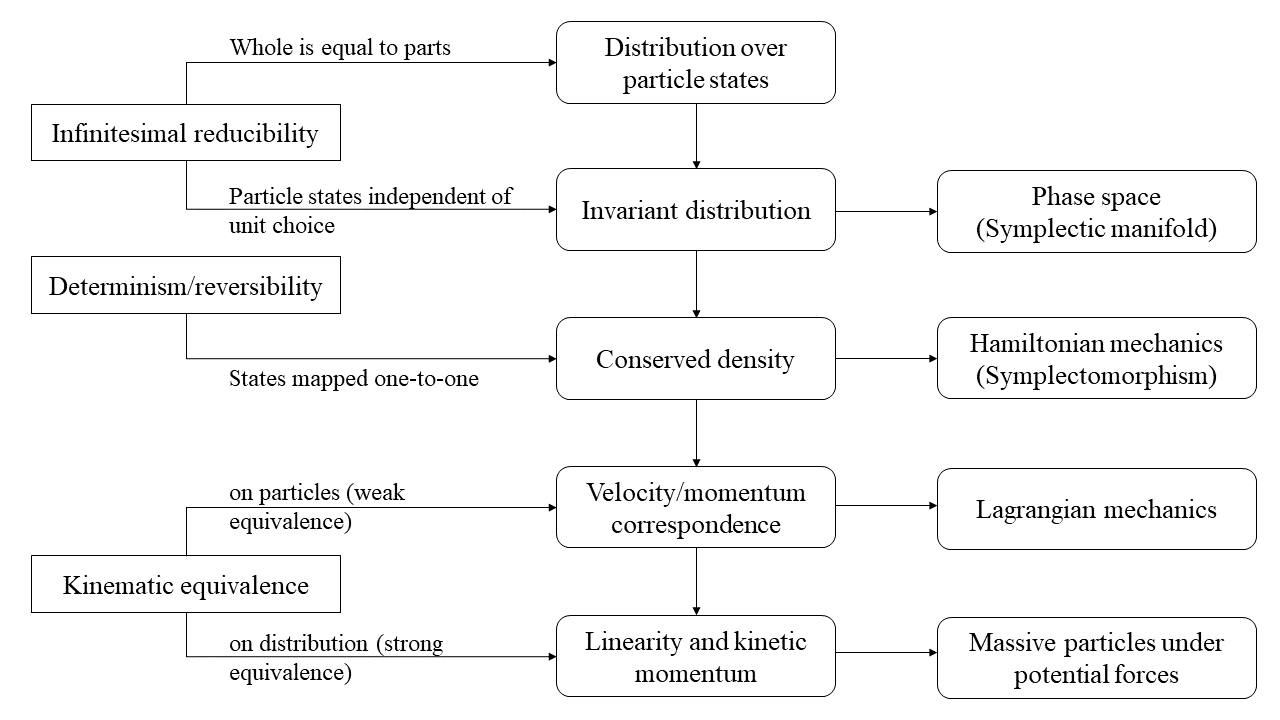
\includegraphics[width=\columnwidth]{images/ClassicalDiagram.png}
	\caption{Assumptions for classical mechanics}\label{fig_classical_diagram}
\end{figure}

The three assumptions lie on the left column. Each assumption leads to one or two key insights that progressively lead to the physical concepts in the middle column. Each of these is then mapped to its corresponding formal framework on the right.

\subsection{Classical phase space}

Classical phase space is recovered under the:
\begin{assump}[Infinitesimal reducibility]
	The state of the system is reducible to the state of its infinitesimal parts. That is, giving the state of the whole system is equivalent to giving the state of its parts, which in turn is equivalent to giving the state of its subparts and so on.
\end{assump}

Under this assumption, the state of the whole is a distribution over the states of the parts. More precisely, let $\mathcal{C}$ be the state space for the whole system. We call particle the limit of recursive subdivision. Let $\mathcal{S}$ be the state space for the particles. Then for each $c \in \mathcal{C}$ we can find one and only one $\rho_c : \mathcal{S} \to \mathbb{R} $ that describes the state of its parts. That is, the state of the whole is a distribution over the infinitesimal parts. If $\mathcal{S}$ is a manifold, $\int_U \rho_c d\mathcal{S}$ gives us the fraction of the system whose parts are in the region $U$ of the state space.

The next step takes the rest of the section. We need to show that $\mathcal{S}$ has the structure of phase space, with its conjugate variables. Mathematically, $\mathcal{S}$ is a symplectic manifold. The key insight is that, on a manifold, $\rho_c$ must transform both as a scalar function (the value must depend on the point and not on the coordinates) and as a density. Classical phase space is the only space that allows these invariant distributions.

The key concept is to keep track of the unit system, so we need precise terminology. We call state variables a set of quantities $\xi^a$ that fully identify a state.\footnote{In mathematical terminology, these are the coordinates of the manifold.} That is, we can write each state $s(\xi^a)$ as a function of the state variables. We call coordinate $q \in \xi^a$ a particular variable that defines a unit. The key problem is to understand how many coordinates we can have for a given set of state variables.

We start with the simplest case, where one coordinate is sufficient to define the unit system, which means the following four conditions:
\begin{enumerate}[noitemsep]
	\item the state variables can be written as $\xi^a = \{ q, k^i \}$
	\item we can arbitrarily change coordinate to $\hat{q}=\hat{q}(q)$
	\item a change of coordinate induces a unique change over the remaining state variables $\hat{k}^j = \hat{k}^j(q, k^i)$
	\item the density is the same regardless of the coordinates used.
\end{enumerate}

Now we show that there can only be one $k^i$. Suppose we change unit $\hat{q}=\hat{q}(q)$. Call the new units $\hat{\xi}^b = \{ \hat{q}, \hat{k}^j\}$. We have $\rho_c(\hat{\xi}^b)=\rho_c(s(\hat{\xi}^b))=\rho_c(s(\xi^a))=\rho_c(\xi^a) = \left|\frac{\partial \hat{\xi}^b}{\partial \xi^a} \right| \rho_c(\hat\xi^b)$. Therefore the Jacobian $\left|\frac{\partial \hat{\xi}^b}{\partial \xi^a} \right|$ must be equal to 1. Note that, since $\hat{q}$ depends only on $q$, $\left|\frac{\partial \hat{\xi}^b}{\partial \xi^a} \right| = \left|\frac{\partial \hat q}{\partial q} \right|\left|\frac{\partial \hat{k}^j}{\partial k^i} \right|$. Suppose there is only one variable. Then we would have $\left|\frac{\partial \hat q}{\partial q} \right| = 1$. But this would mean the unit change cannot be arbitrary. Therefore we must have two or more variables and therefore $\left|\frac{\partial \hat{k}^b}{\partial k^a} \right| = \left|\frac{\partial q}{\partial \hat q} \right|$. This puts a constraint only on the determinant of the transformation. Suppose there are three or more variables. This constraint is not enough to recover the transformation uniquely and therefore $\hat q$  would not fully define the units for all other state variables. This means there must be two variables: $q$ and a single $k$. Coordinate independent areas and densities can only be defined on a two-dimensional manifold.

Now we generalize to multiple coordinates. We say two coordinates are independent if changing the units for one does not induce a change of units for the other. Now suppose our particle state space $\mathcal{S}$ is such that its units are fully defined by $n$ independent coordinates $q^i$. Suppose you change the first coordinate $q^1$ without changing the others. Then we will find a variable $k_1$ that changes as before so that the densities are invariant. Now change the second coordinate $q^2$ in the same way while also fixing $k_1$. Then we find a corresponding $k_2$. We can proceed in the same way until we exhaust all coordinates, which must also mean that there are no state variables left. We find that $\mathcal{S}$ is $2n$-dimensional, and the state variables are $\xi^a = \{ q^i, k_i \}$. We define an independent degree of freedom as the space charted by a pair of such variables.

We can dress the result a bit more formally, and show that $\mathcal{S}$ is a symplectic manifold. To characterize marginal distributions on each degree of freedom, we want to define integrals of the form $\int_{\Sigma} \rho_c \omega(d\Sigma)$ such that the density $\rho_c$ is invariant. Therefore we need a two-form $\omega$ that assigns an infinitesimal area to each infinitesimal surface, and we need $\omega$ to be invariant. Because degrees of freedom are, at least locally, independent, the total number of states in a volume is the product of the possible configurations of each degree of freedom. This means the volume form is proportional to $\omega^n$. This cannot be degenerate (i.e.~it must be nonzero for each infinitesimal volume) since all regions of phase space must, by definition, contain some states.. Therefore $\omega$ itself cannot be degenerate. As the degrees of freedom are independent, the number of states on a surface does not change if we translate it across independent degrees of freedom. If we imagine a parallelepiped, the integral over the surface must be zero (integrals over opposite sides are equal and opposite). Therefore $\mathcal{S}$ must come equipped with a two-form $\omega$ that is closed and not degenerate and therefore $\mathcal{S}$ is a symplectic manifold. By convention, we set $\omega = \hbar dq^i \wedge dk_i = dq^i \wedge dp_i$ where $p_i = \hbar k_i$.

The conclusion is that, under the infinitesimal reducibility assumption, the state space of the system is a coordinate invariant distribution over the state space of the infinitesimal parts. If the state space of the particles is a manifold, then it is a symplectic manifold, which is the only type of manifold that supports coordinate invariant distributions.

\subsection{Classical Hamiltonian mechanics}

Having recovered the classical state space, the law of evolution can be recovered with the following:
\begin{assump}[Deterministic and reversible evolution]\label{assump_detrev}
	Given the present state of the system, all future (determinism) and past (reversibility) states are uniquely identified.
\end{assump}

We first apply the assumptions to the motion of a single particle. Let $\lambda : \mathbb{R} \to \mathcal{S}$ be the evolution over time of the state of a particle. Under the assumption, this will be uniquely identified by the initial state $s_0 = \lambda(t_0)$ at the initial time $t_0$. Secondly, we apply the assumption to the density in the sense that all the particles that start with the same initial state must end up in the same final state and vice-versa. That is, if $\rho(\lambda(t_0), t_0)$ is the density associated to the initial particle at the initial time, we must have that $\rho(\lambda(t), t) = \rho(\lambda(t_0), t_0)$: the density must remain the same throughout the evolution.

Now consider the integral $\int_{\Sigma} \rho \omega(d\Sigma)$. Both the region and the density will be mapped in time to $\hat{\Sigma}$ and $\hat{\rho}$ respectively. The fraction of the system found in the new region will have to be the same as the one found in the old region. That is, $\int_{\Sigma} \rho \omega(d\Sigma) = \int_{\hat{\Sigma}} \rho \hat{\omega}(d\hat{\Sigma})$. Since both the integral and the density have to remain constant during the evolution, then $\omega$ will need to remain the same. That is, the areas in phase space must be mapped to areas of equal size and independent degrees of freedom must be mapped to independent degrees of freedom (or volumes would not be mapped to equal volumes). The evolution is a symplectomorphism and corresponds to Hamiltonian evolution. Intuitively, this is the inverse of Liouville's theorem: instead of positing Hamiltonian evolution and finding conservation of areas and volumes, deterministic and reversible evolution imposes the conservation of areas and volumes which leads to Hamiltonian evolution.

The argument can also be constructed through statistical concepts (i.e.~determinism and reversibility means conservation of variance), thermodynamic concepts (i.e.~determinism and reversibility means only the state of the system is important for the evolution; the system is therefore isolated and must conserve energy) or information theoretic consideration (i.e.~under deterministic and reversible evolution the amount of information does not change, so information entropy has to be conserved).

Other notable results:
\begin{itemize}
	\item phase space is the only space upon which information entropy is coordinate independent and Hamiltonian evolution is precisely the evolution that preserves information entropy
	\item we can construct a classical analogue of the uncertainty principle
	\item the extension to relavistic mechanics only requires proper handling of the time coordinate (and no additional assumptions)
\end{itemize}

\subsection{Geometry of Hamiltonian/Lagrangian mechanics}

The geometry of both Hamiltonian and Lagrangian mechanics can best be understood in the phase space where time is added. This is technically a contact manifold.

For one degree of freedom, we can use standard 3D differential calculus. We have $\xi^a=\{q,p,t\}$, $S^a=\{\frac{dq}{dt},\frac{dp}{dt},\frac{dt}{dt}\}$ and $\theta_a=\{p,0,-H\}$. Note that $\omega = -d \theta$. The equations of motion are given by $S=-curl(\theta)$ and the Lagrangian by $L=\theta \cdot S$. In fact, $curl(\theta)=\{\partial_p \theta_t - \partial_t \theta_p, \partial_t \theta_q - \partial_q \theta_t, \partial_q \theta_p - \partial_p \theta_q\} = \{ -\partial_p H , \partial_q H , - 1 \}$ and $L = \frac{dq}{dt}p - \frac{dt}{dt}H$.

To generalize, we can set $\xi^a=\{q^i,p_i,t\}$, $S^a=\{\frac{dq^i}{dt},\frac{dp_i}{dt},\frac{dt}{dt}\}$ and $\theta_a=\{p_i,0,-H\}$. The Lagrangian is still $L=\theta \cdot S = S^a \theta_a = \frac{dq^i}{dt}p_i - \frac{dt}{dt}H$. The equations of motion should be $d\theta(S, \cdot ) = 0$. In fact, $d\theta = \partial_a \theta_b e^a \wedge e^b = (\partial_a \theta_b - \partial_b \theta_a) e^a \otimes e^b$.
\begin{equation*}
(d\theta)_{ab} = \begin{bmatrix}
0 & \delta^j_i & - \partial_{q^i} H \\
-\delta^i_j & 0 & - \partial_{p_i} H \\
\partial_{q^j} H & \partial_{p_j} H & 0
\end{bmatrix}
\end{equation*}
We find
\begin{align*}
d\theta(S, \cdot )  &= S^a (d\theta)_{ab} e^b = 0 \\
&= (S^{q^i}(d\theta)_{q^ib} + S^{p_i}(d\theta)_{p_ib} + S^{t}(d\theta)_{tb}) e^b \\
&= (S^{q^i}(d\theta)_{q^iq^j} + S^{p_i}(d\theta)_{p_iq^j} + S^{t}(d\theta)_{tq^j}) e^{q^j} + \\
& (S^{q^i}(d\theta)_{q^ip_j} +  S^{p_i}(d\theta)_{p_ip_j} + S^{t}(d\theta)_{tp_j}) e^{p_j} + \\
& (S^{q^i}(d\theta)_{q^it} + S^{p_i}(d\theta)_{p_it} + S^{t}(d\theta)_{tt}) e^t \\
&= (-S^{p_i}\delta^i_j + S^{t}\partial_{q^j} H ) e^{q^j} + \\
& (S^{q^i}\delta^j_i +  S^{t}\partial_{p_j} H) e^{p_j} + \\
& (-S^{q^i} \partial_{q^i} H - S^{p_i} \partial_{p_i} H) e^t \\
\end{align*}
\begin{align*}
S^{p_j} &= S^{t} \partial_{q^j} H \\
S^{q^j} &= - S^{t}\partial_{p_j} H \\
-S^{q^i} \partial_{q^i} H - S^{p_i} \partial_{p_i} H &= S^{t}\partial_{p_i} H \partial_{q^i} H - S^{t} \partial_{q^i} H \partial_{p_i} H = 0
\end{align*}
Note that the last expression is not a new equation: it is identical to zero given the previous two equations.

The equation $- d\theta(S, \cdot ) = \omega(S, \cdot ) = 0$ tells us that the displacement is the only direction that does not contribute states. Therefore the area given by $\omega$ of any surface tangent to the displacement field is zero. The action principle is just a straight consequence of this.

The interesting aspect is that a pseudo-Lagrangian with the associated action principle always exists even in the case where it cannot be expressed as a function of $q$ and $\dot q$. That is, an action principle always works for trajectories in $\{q(t), p(t)\}$.

\subsection{Classical massive particles under potential forces}

Having recovered classical Hamiltonian mechanics, we can further restrict the law of evolution with the following:

\begin{assump}[Kinematic equivalence]
	The kinematics of the system (i.e. trajectories in physical space-time) is enough to recover its dynamics (i.e. evolutions in state space).
\end{assump}


First, as before, we apply the assumption to the particles, which means that for every evolution in phase space there should be one and only one trajectory. Note that each space variable $x^i$ is a coordinate, i.e. a state variable that defines a unit. In fact, the trajectories can be fully described by those units and only those units. So we can say that $q^i=x^i$, each $q^i$ will be paired with a conjugate $p_i$ and each state $\{q^i, p_i\}$ will be mapped to one and only one trajectory. At each point $x^i$, then, infinitely many trajectories must pass, one for each combination of $\{p_i\}$. Since the trajectories are differentiable in $x^i$, we can define a velocity $v^i = d_t x^i$. If the equations of motion were such that $v^i=v^i(q^i)$, then kinematic equivalence would fail as the full trajectory would be determined only by $q^i$. So we must have $v^i=v^i(q^i, p_i)$. The relationship must be invertible or kinematic equivalence would fail. At any given time, then, we must have the following relationship:
\begin{equation}
\begin{aligned}
x^i &= q^i \\
v^j &= d_t x^j = v^j(q^i, p_k)
\end{aligned}
\end{equation}

Let us call weak equivalence the notion that $v^j(q^i, p_k)$ must be invertible at every $q^i$ and therefore we can write $p_k= p_k(x^i, v^j)$ as a function of position and velocity. In this case, the Jacobian matrix  $\frac{\partial v^j}{\partial p_k}$ must be invertible. Since $v^j = d_t q^j = \frac{\partial H}{\partial p_j}$, the Hessian $\frac{\partial^2 H}{\partial p_k \partial p_j}$ must be nonzero everywhere, and therefore must have the same sign which we take to be positive. In this case, and only in this case, we can construct a Lagrangian from a Hamiltonian:
\begin{equation}
L(x^i, v^j) = v^k p_k (x^i, v^j) - H(q^i(x^i), p_k(x^i, v^j))
\end{equation}
These are also exactly the cases where the Lagrangian, using the principle of minimal action, leads to a unique solution.

Now we look at the whole distribution and how it can be expressed as a function of position and velocity. We have $\rho(q^i, p_j) = |J| \rho(x^i, v^j) = \left|\frac{\partial v^i}{\partial p_j}\right| \rho(x^i, v^j)$ since
\begin{equation}
\begin{aligned}
|J| &= \begin{vmatrix}
\frac{\partial x^i}{\partial q^j} & \frac{\partial x^i}{\partial p_j} \\
\frac{\partial v^i}{\partial q^j} & \frac{\partial v^i}{\partial p_j}
\end{vmatrix}
= \begin{vmatrix}
\delta^i_j & 0 \\
\frac{\partial v^i}{\partial q^j} & \frac{\partial v^i}{\partial p_j}
\end{vmatrix} \\
&= \left|\delta^i_j\right| \left|\frac{\partial v^i}{\partial p_j}\right| - \left|0\right| \left|\frac{\partial v^i}{\partial q^j}\right|
= \left|\frac{\partial v^i}{\partial p_j}\right|.
\end{aligned}
\end{equation}
Note that while the value given by $\rho(q^i, p_j)$ is coordinate independent, the value given by $\rho(x^i, v^j)$ depends on the choice of coordinate through $\left|\frac{\partial v^i}{\partial p_j}\right|$. If $x^i$ truly sets the unit system by itself, then $\left|\frac{\partial v^i}{\partial p_j}\right|$ must be a function of position only. Similar considerations will also hold for marginal distributions (i.e.~distributions on a subset of the coordinates) which means all components of $\frac{\partial v^i}{\partial p_j}$ must be a function of position only. We set:
\begin{equation}
\begin{aligned}
\frac{\partial v^i}{\partial p_j} = \frac{1}{m} g^{ij} \\
\frac{\partial p_j}{\partial v^i} = m g_{ji}
\end{aligned}
\end{equation}
where $m$ is the unit conversion constant between velocity and conjugate momentum while $g_{ij}$ represents the linear dependency.

If we integrate, we have:
\begin{equation}
\begin{aligned}
v^i = \frac{1}{m} g^{ij}(p_j - A_j) \\
p_j = m g_{ji} v^i + A_j
\end{aligned}
\end{equation}
where $A_j$ are arbitrary functions. Note that:
\begin{equation}
v^i = d_t q^i = \frac{\partial H }{\partial p_i} = \frac{1}{m} g^{ij}(p_j - A_j) \\
\end{equation}
We integrate yet again and find:
\begin{equation}
H = \frac{1}{2m} (p_j - A_j) g^{ij}(p_j - A_j) + V \\
\end{equation}
where V is another arbitrary function. We recognize this as the Hamiltonian for massive particles under potential forces.

Kinematic equivalence, then, severely constrains the Hamiltonian and gives a physical justification as to why Hamiltonian of that forms are the most important at a fundamental level. They are the ones where all the dynamics is contained in purely kinematic degrees of freedom.

\section{Quantum mechanics and irreducibility}

Quantum mechanics can be recovered swapping reducibility with irreducibility as shown in diagram \ref{fig_quantum_diagram}, which can be used as a guide throughout this section.

\begin{figure}[h]
	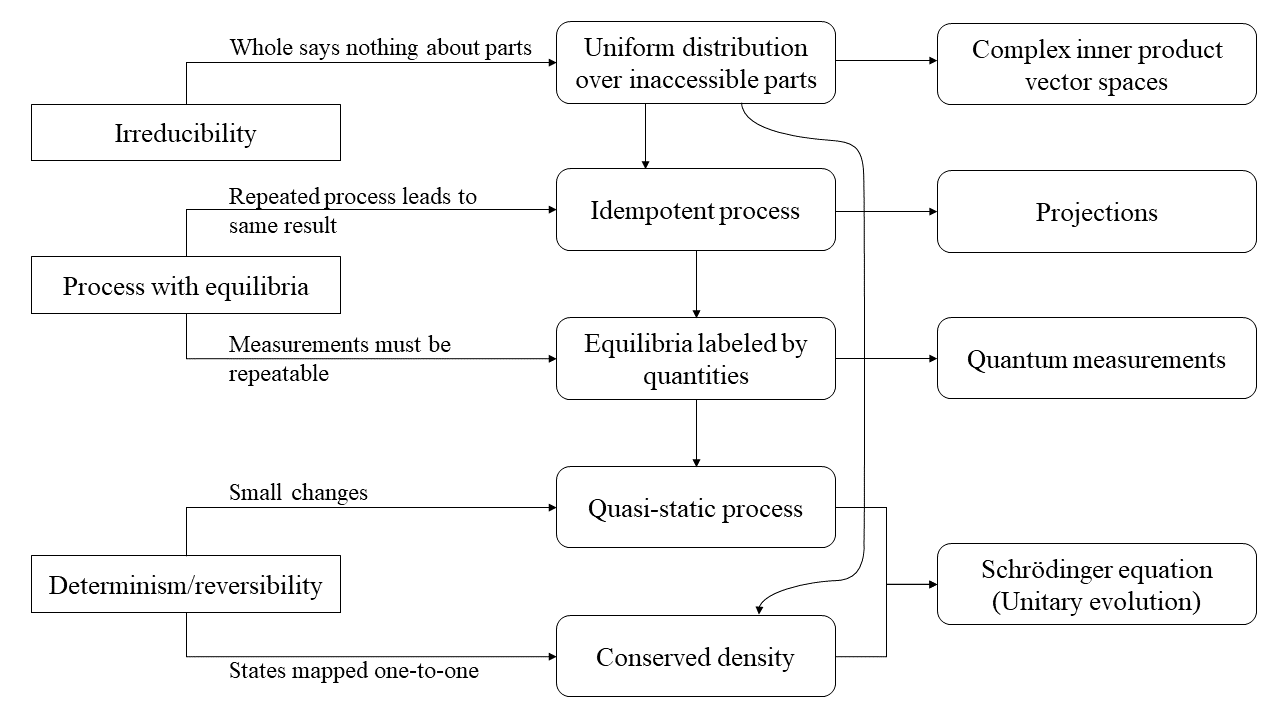
\includegraphics[width=\columnwidth]{images/QuantumDiagram.png}
	\caption{Assumptions for quantum mechanics}\label{fig_quantum_diagram}
\end{figure}

The assumptions lie on the left column. Each assumption leads to one or two key insights that progressively lead to the physical concepts in the middle column. Each of these is then mapped to its corresponding formal framework on the right. Note that ``quasi-static process'' and ``conserved density'' both independently lead to the same result of ``unitary evolution''.

\subsection{Irreducibility}

The state space of quantum mechanics can be recovered under the:

\begin{assump}[Irreducibility]
	The state of the system is irreducible. That is, giving the state of the whole system says nothing about the state of its parts.
\end{assump}

Under this assumption the state of the system is automatically an ensemble over the state of the parts as preparation of the whole leaves the parts unspecified. For the same reason, the entropy of these ensembles must be the same, or some ensembles would provide more or less information about the parts. The whole task, then, is to characterize these ensembles without making specific assumptions on the parts.

Let $\mathcal{C}$ be the state space of the irreducible system. Let us call fragment a part of the irreducible system. The state of a fragment will be associated with a random variable uniformly distributed over the possible fragment states. As discussed in the context of classical mechanics(CITE), distributions over states must be invariant and symplectic manifolds are the only manifolds over which invariant distributions can be defined. As we cannot say anything about the state of the fragments, the dimensionality of this manifold must be irrelevant as long as it is even dimensional. For simplicity, we can choose a two-dimensional one. Therefore we are interested in the space of bi-dimensional uniform distributions formed by a pair of two random variables $A$ and $B$.

The values of the variables themselves are not relevant, as they are not physically accessible by assumption. However, the size of the system $\mu = \int \rho dA \wedge dB$ is relevant. Without loss of generality, we can rescale $A$ and $B$ such that the density $\rho$ is not only uniform but unitary: $\rho = 1$. This way the size of the system is directly proportional to the area covered by the random variables. In other words: the more fragments there are, the more each fragment can swap its state with another without changing the whole, the more uncertainty there is on the state of the fragment, the higher the variance of the random variables.

Since only linear transformations will preserve the uniform distribution, we look to those. These are translations, stretches and rotations. Translations do not lead to other physically distinguishable states since the exact values of $A$ and $B$ are not physically accessible. Stretching of the distribution will correspond to an increase of the size of the system, which is physically accessible. However, only the stretching of the area is of interest. So, without loss of generality, we can set $\sigma_A = \sigma_B = \sigma$ and we have $\mu \propto \sigma^2$. Rotations just change the correlations which, by themselves, are not physically accessible. However, under addition the correlations still result in differences in variance and, indirectly, the size of the system, and therefore are physically interesting. The space of transformations is therefore given by two parameters $a$ and $b$ such that:
\begin{equation}
\begin{aligned}
C &= a A + b B \\
D &= -b A + a B
\end{aligned}
\end{equation}
Equivalently, we can use the complex number $c = a + \imath b$ to characterize the transformation, which we can note as $\tau(c)$. The increase/decrease in size is given by $a^2 + b^2 = (a - \imath b) (a + \imath b) = c^* c$ and the change in correlation is given by the Pearson correlation coefficient $\rho_{A,\tau(c) A} = \cos \arg c$.

Putting it all together, we can characterize the state space $\mathcal{C}$ with a complex vector space. The linear combination represents the mixing of the different stochastic descriptions. Two vectors that only differ by a total phase are physically equivalent since a global change of correlation does not change the distribution.

We can define a scalar product $\langle \cdot | \cdot \rangle$ where the square norm induced corresponds to the size of the system (or equivalently to the strength of the random variable) and the phase difference corresponds to the correlations (the Pearson correlation coefficient). To see this, note the formal equivalence between the variance and norm rules under linear composition:
\begin{equation}
\begin{aligned}
\sigma^2_{X+Y} &= \sigma^2_{X} + \sigma^2_{Y} + 2 \, \sigma_{X} \sigma_{Y} \rho_{X,Y} \\
|\psi+\phi|^2&=|\psi|^2 + |\phi|^2 + 2 |\psi||\phi|\cos(\Delta \theta)
\end{aligned}
\end{equation}
The quadratic form, again, reflects the fact that the size of the system is proportional to the variance of a random variable. Since the size of the system is fixed, we use unitary vectors to represent actual states. The state of the system, then, is represented by a ray in a complex inner product space.

Lastly, we need to define an expectation operator that returns the average value for each physical quantity. This operator will have to be linear under linear combination of quantities:
\begin{equation}
E[aX + bY | \psi] = aE[X | \psi] + bE[Y | \psi].
\end{equation}
It will not be linear under linear combination of states:
\begin{equation}
E[X | \psi + \phi] \neq E[X | \psi] + E[X | \phi].
\end{equation}
Yet, it will have to be proportional to the increase in size and invariant under a total change in correlation: $E[X | \tau(c) \psi] = c^*c E[X | \psi]$. This leads us to associate to each physical quantity a linear Hermitian operator $X$ where $E[X | \psi] = \langle \psi | X | \psi \rangle$. An eigenstate $\psi_0$ of $X$ corresponds to a state where all the elements of the ensemble have exactly the same value. That is, $E[(X - \bar{x})^2 | \psi_0] = 0$.

Note that an inner product space can always be completed into a Hilbert space. This may, however, bring in objects that may not correspond to physical objects (i.e. infinite expectation for some quantities). In general, we believe it is better to regard the (possibly incomplete) inner product space as the physical state space and regard the completion as a mathematical device for calculation. For example, the Schwartz space seems more physically meaningful than the standard $L^2$ space as it gives finite expectation of all polynomials of position and momentum and, moreover, it is closed under Fourier transform.

\subsection{Process with equilibria}

The first type of process we consider is one with equilibria. The measurement process is recovered as a special case.

\begin{assump}[Process with equilibria]
	Given an initial ensemble (i.e.~mixed state), the final ensemble is uniquely determined and remains the same if the process is applied again.
\end{assump}

Under this assumption, the process can be characterized by a projection operator. Let $\rho_1$ be the density matrix that characterizes a mixed state. Since the final mixed state must be uniquely determined by $\rho_1$, it will be $\mathcal{P}(\rho_1)$ for some operator $\mathcal{P}$. Similarly, if $\rho_2$ is another initial mixed state, its final operator will be $\mathcal{P}(\rho_2)$. Note that, given any observable $X$ the expectation $E[X|\rho_1] = \tr(X\rho_1)$ is the trace of $X\rho_1$. Similarly $E[X|\mathcal{P}(\rho_1)] = \tr(X \mathcal{P}(\rho_1))$.

We can always create statistical mixtures of the ensembles and we must have $E[X|a \rho_1 + b \rho_2] = a E[X|\rho_1] + b E[X|\rho_2]$ since these are classical mixtures. But since these are classical mixtures, the final state will also need to obey $E[X|a \mathcal{P}(\rho_1) + b \mathcal{P}(\rho_2)] = a E[X|\mathcal{P}(\rho_1)] + b E[X|\mathcal{P}(\rho_2)]$ for all possible $X$. Which means $\mathcal{P}(a \rho_1 + b \rho_2) = a \mathcal{P}(\rho_1) + b \mathcal{P}(\rho_2)$ Therefore the operator $\mathcal{P}$ is a linear operator. Moreover, the process applied twice must lead to the same result, which means $\mathcal{P}(\mathcal{P}(\rho)) = \mathcal{P}(\rho)$ for any $\rho$. That is, $\mathcal{P}^2 = \mathcal{P}$. Therefore $\mathcal{P}$ is a projection.

Suppose, now, that we want to measure a quantity $X$. We want the final outcome, the final ensemble, to be determined by the initial state, the initial ensemble. We also want the measurement to be consistent in the sense that, if it is repeated immediately after, it should yield the same result. Therefore the process will be a projection. We will also want that the process does not distort the quantity. That is, $E[X|\rho] = E[X|\mathcal{P}(\rho)]$. This means that the eigenstates of $X$ will correspond to equilibria of the process. Moreover, subsequent measurements must give the same value, not just the same mixture. That is, if $X_1$ is the random variable after the first instance of the process and $X_2$ is the random variable after the second instance, $P(X_2 = x| X_1 = x ) = 1$. This means that $E[(X - \bar{x})^2|\mathcal{P}(\rho)] = 0$ which means the eigenstates of $X$ are the only equilibria.

The measurement process is therefore simply a special case of a process with equilibria.

\subsection{Deterministic and reversible evolution}

The second type of process we consider is one that is deterministic and reversible, which is the same as assumption \ref{assump_detrev}.

Under this assumption, the process can be characterized by unitary evolution (i.e.~the Schrodinger equation). There are multiple different ways to see this. The first relates to the more general idea that all deterministic and reversible processes must be isomorphisms in the category of states. Since the state space is an inner product space, the isomorphism is unitary evolution.

The second, is that if there is a set of quantities $X_0$ at time $t_0$ that fully identify the state (i.e. the state is the only eigenstate of those quantities), then there must be a corresponding set of quantities $X_1$ that fully identify the state at time $t_1$. This means that the evolution maps basis to basis. Moreover, given the linearity of statistical mixtures, this will also mean that a statistical distribution over $X_0$ will have to map to the same distribution over $X_1$. Therefore the evolution must map linear combinations of that basis to the same linear combination. The evolution is a linear operator. Since the total size of the irreducible system cannot change, the operator must be unitary.

The third, is by constructing a quasi-static process from processes with equilibria, much like one does in thermodynamics.  The idea is that we have an infinitesimal time step, an initial state $\psi_t$ and a final state $\psi_{t+dt}$. We want $P(\psi_{t+dt} | \psi_t ) = 1$. This means that $|\langle \psi_{t+dt} | \psi_{t} \rangle|^2 = 1$. This can happen only if the difference between initial and final states is infinitesimal. That is, $\langle \psi_{t+dt} | \psi_{t} \rangle = 1 + \imath \epsilon dt$ where $\epsilon$ is a real number. Therefore, by convention, we can write $| \psi_{t+dt} \rangle = I + \frac{H dt}{\imath \hbar} | \psi_{t} \rangle$ where $H$ is a Hermitian operator.

Putting these perspectives together, time evolution is a unitary operator which can be written as $U=e^{\frac{H\Delta t}{\imath \hbar}}$. If we start in an eigenstate of $X$, that is $X | \psi_t \rangle = x_0 | \psi_t \rangle$ we will end in an eigenstate $\hat{X} | \psi_{t + \Delta t} \rangle = x_0 | \psi_{t + \Delta t} \rangle$ of another operator $\hat{X} = e^{\frac{H\Delta t}{\imath \hbar}} X e^{- \frac{H\Delta t}{\imath \hbar}}$.

In fact:
\begin{equation}
\begin{aligned}
e^{\frac{H\Delta t}{\imath \hbar}} X e^{- \frac{H\Delta t}{\imath \hbar}}| \psi_{t + \Delta t} \rangle
&= e^{\frac{H\Delta t}{\imath \hbar}} X e^{- \frac{H\Delta t}{\imath \hbar}} U | \psi_t \rangle \\
&= e^{\frac{H\Delta t}{\imath \hbar}} X e^{- \frac{H\Delta t}{\imath \hbar}} e^{\frac{H\Delta t}{\imath \hbar}} | \psi_t \rangle \\
&= e^{\frac{H\Delta t}{\imath \hbar}} X  | \psi_t \rangle \\
&= e^{\frac{H\Delta t}{\imath \hbar}} x_0  | \psi_t \rangle \\
&= x_0 U | \psi_t \rangle \\
&= x_0 | \psi_{t + \Delta t} \rangle
\end{aligned}
\end{equation}
This is consistent with assuming there is a quasi-static process that, at every $t$, has equilibria identified by $e^{\frac{H (t - t_0)}{\imath \hbar}} X e^{- \frac{H (t - t_0)}{\imath \hbar}}$. Note that, unlike thermodynamics, the equilibria during the evolution are not set by external constraints but by the system itself. That is, $X$ depends on the initial state of the system.

In this light, the measurement processes and the unitary processes can be seen as particular cases of the same type of processes, those with equilibria, which are defined as a black-box from initial to final state. This is consistent with the irreducibility assumption as the inability to describe the dynamics of the parts implicitly assumes that the dynamics of the parts is at equilibrium and sets a time-scale under which the further description of the system (i.e. non-equilibrium dynamics) would require describing the internal dynamics.

\section{Open questions and possible extensions}

\subsection{Directional degrees of freedom}

Suppose we we want to assign a degree of freedom to a direction within an $n$-dimensional physical space. Choosing a direction is the same as choosing a point on the $(n-1)$-dimensional sphere. Since degrees of freedom must be two-dimensional, the sphere must be two-dimensional. Furthermore, the only sphere that can be a symplectic manifold is the two dimensional sphere, which means the only spaces where a direction can correspond to an independent degree of freedom are three dimensional.

To find a pair of conjugate variables, consider the solid angle $d\Omega=\sin \varphi_z d\varphi_z d\theta^{xy}$ where $\varphi_z$ is the azimuthal angle. This is a quantity that is dimensionless and that is proportional to the number of possible directions, therefore we can use it as a measure for the possible configurations. We can express the two form for our space as $\omega(d\theta^{xy}, d\varphi_z) = \hbar d\Omega = \hbar\sin \varphi_z d\varphi_z d\theta^{xy} = d(- \hbar \cos \varphi_z ) \wedge d\theta^{xy} = d\theta^{xy} \wedge d(\hbar \cos \varphi_z )$. Set $S_z= \hbar \cos \varphi_z$ as the component of the normalized vector multiplied by $\hbar$. We have that $\omega(d\theta^{xy}, dS_z) = d\theta^{xy} \wedge dS_z$ therefore $\theta^{xy}$ and $S_z$ are conjugate variables. Which means $\{ \theta^{xy}, S_z \} = 1$

We can now write all the components of the vector in terms of the conjugate variables.
\begin{align*}
S_x &= \hbar \sin \varphi_z \cos \theta^{xy} = \sqrt{\hbar^2 - S_z^2} \cos \theta^{xy}  \\
S_y &= \hbar \sin \varphi_z \sin \theta^{xy} = \sqrt{\hbar^2 - S_z^2} \sin \theta^{xy}\\
S_z &= \hbar \cos \varphi_z = S_z
\end{align*}
These relationships can be used to calculate the Poisson brackets across components. One can then study the motion under a simple linear Hamiltonian $H = B^i S_i$.

What needs to be understood is how this generalizes to the relativistic case.


\subsection{Curvature for particle dynamics}

The assumption of kinematic equivalence already gives us relativistic Hamiltonians. Does it also give us a relationship between the curvature of the metric tensor and the forces acting on the particles?

The setup is the following. Suppose we have two vectors in the extended phase space $d\xi^a = \{dq^\alpha, 0\}$ and $d\nu^a = \{0, dp_\alpha\}$. Using the symplectic form we have the invariant $d\xi^a \omega_{ab}d\nu^b = dq^\alpha dp_\alpha$. Under the kinematic assumption we have $dq^\alpha = dx^\alpha$ and $dp_\alpha = mg_{\alpha\beta}du^\beta + q A_\alpha$. We have $d\xi^a \omega_{ab}d\nu^b = dx^\alpha m g_{\alpha\beta} du^\beta + dx^\alpha q A_\alpha$.

Since the two terms have to match at each point and the symplectic form has the same components at each point, can we constrain the change of the components of $g_{\alpha\beta}$? The general idea would be that components of $g_{\alpha\beta}$ may have to change in space/time coordinately with $A_\alpha$ as to make $d\xi^a \omega_{ab}d\nu^b = dq^\alpha dp_\alpha$ remain the same. Note that derivatives in $q^\alpha$ are taken at constant $p_\alpha$ while derivatives in $x^\alpha$ are taken at constant $u^\alpha$.

\subsection{Thermodynamics}

The current thoughts to recover thermodynamics are based on the work on states and processes within the general theory, which tells us that we can define state spaces only for systems that can, at least in some processes, be described independently from the rest. The process entropy, which in general is defined only for a specific process, can be abstracted and become associated with the states themselves. Therefore we have an equation of state $S(\xi^a)$ where $\xi^a$ form a set of variables that fully identify the state. Moreover, one finds that the state entropy is additive under system composition of independent systems.

In a process with equilibria different evolutions must converge to the same final state, which means the process entropy increases and is maximized at equilibria. This gives the general idea that entropy increases during an irreversible process. These results are therefore valid in general, no matter what type of system is being described.

To find thermodynamics specifically, we need an additional set of assumptions. First, all states are equilibria. Second, all state variables $\xi^a$ are additive under system composition. Third, one of the them, which we call internal energy $U$, is conserved under any evolution, including irreversible evolution. We can then write the equation of state as $S(U, x^i)$ and define the following quantities:
\begin{equation}
\begin{aligned}
\frac{\partial S}{\partial U} &= \beta = \frac{1}{k_B T} \\
\frac{\partial S}{\partial x^i} &= - \beta X_i
\end{aligned}
\end{equation}
We can then express the differentials as:
\begin{equation}
\begin{aligned}
dS &= \frac{\partial S}{\partial U} dU + \frac{\partial S}{\partial x^i} dx^i &= \beta dU - \beta X_i dx^i \\
dU & = T k_B dS + X_i dx^i
\end{aligned}
\end{equation}
This is essentially Gibbs' approach to thermodynamics.

To recover the laws, we need a few more definitions. We define a reservoir $R$ as a system for which the internal energy $U_R$ is the only state variable and the state entropy $S_R$ is a linear function of $U_R$. That is, $\frac{\partial S_R}{\partial U_R} = \beta_R = \frac{1}{k_B T_R}$ is a constant. We call heat $Q=-\Delta U_R$ the energy lost by the reservoir during a transition.

We define a purely mechanical system $M$ as a system for which the state entropy is zero for each state. That is, $S_M(U_M, x^i_M) = 0$. We call work $W = \Delta U_M$ the energy acquired by a purely mechanical system during a transition.

Now, consider a composite system made of a generic system $A$, a reservoir $R$ and a purely mechanical system $M$. Consider a transition where we go to a new equilibrium. Since energy is additive under system composition, let us call $U$ the total energy. Since energy is conserved we have:
\begin{equation}
\begin{aligned}
\Delta U &= 0 = \Delta U_A + \Delta U_R +\Delta U_M = \Delta U_A - Q + W \\
\Delta U_A &= Q - W
\end{aligned}
\end{equation}
Since entropy is extensive, let us call $S$ the total entropy. Since the process is going to an equilibrium, the entropy can only increase. We have:
\begin{equation}
\begin{aligned}
0 &\leq \Delta S = \Delta S_A + \Delta S_R +\Delta S_M = \Delta S_A + \beta_R \Delta U_R + 0 = \Delta S_A + \frac{-Q}{k_B T_R} \\
k_B \Delta S_A &\geq \frac{Q}{T_R}
\end{aligned}
\end{equation}



\iffalse

\chapter{Level of detail}

\section{Granularity}

So far we have studied the properties and constructions that can be defined on top of logical consistency and experimental verifiability. We will now  introduce another primary attribute of statements, the idea that we can compare the level of detail for the description they provide.

We will see that the granularity, the level of detail provided by a statement, cannot be defined in terms of the concepts we previously introduced. We will therefore introduce a new axiom which will allow us to determine which statements provide a finer description and which statement provide the same granularity.

Statement narrowness allows us to say that the statement \statement{the temperature is between 22 and 23 Celsius} is more precise than \statement{the temperature is between 20 and 25 Celsius} but it does not tell us how it compares to \statement{the temperature is between 23 and 25 Celsius}. That is, it can compare only statements that are fully contained in one another, and not statements that are overlapping or incompatible. Ideally, we want to say that \statement{the temperature is between 23 and 25 Celsius} is coarser than \statement{the temperature is between 22 and 23 Celsius}. Saying that the first statements, in fact, is true constrains us to more possibilities than saying that the second is true. It would seem we simply need to keep track quantity intervals or possibility counts, but this does not work. Let's understand what the problems are.

We may think that, at least in the discrete case, we could simply count the possibilities compatible with each statement: the more possibilities, the more the statement is coarser. If two statements are the disjunctions of the same number of possibilities they are of the same granularity. This does not always work. For example, suppose we have a bowl that can contain apples. The domain that counts how many apples are in the bowl will have \statement{there are 2 apples in the bowl} and \statement{there are 5 apples in the bowl} as possibilities. We would be tempted to say they provide the same level of description. Now suppose we extend the domain to count how many of the apples are green. This will have \statement{there are 2 apples in the bowl 1 of which is green} and \statement{there are 5 apples in the bowl 3 of which are green} as possibilities. We would be tempted to say that these too provide the same level of description as each other. But because the two quantities are not independent (i.e. you cannot have more green apples than apples in the bowl) this cannot work. The statement \statement{there are 2 apples in the bowl} would be equivalent to the disjunctions of 3 possibilities in the combined domain: 0, 1 or 2 green apples. The statement \statement{there are 5 apples in the bowl} would be equivalent to the disjunction of 6 possibilities in the combined domain: 0, 1, 2, 3, 4 or 5 green apples. Therefore, it would seem that the second statement covers twice as many cases of the first, so it should be coarser than the first. But if we counted the possibilities in the first domain they were equigranular. So the issue that, depending on the domain, the same statement can break up into a different number of possibilities. Something else needs to tell us which possibilities provide the same level of description.

%TODO: add picture for the apple example

In the continuous case, simply using the cardinality of the possibilities would lead us to say that \statement{the temperature is between 22 and 23 Celsius} and \statement{the temperature is between 20 and 25 Celsius} give us similar description: they both correspond to continuously many possibilities. We may think that using the numeric interval would work, but this also fails in unexpected ways. For example, we may be tempted to say that \statement{the horizontal position of the ball is between 0 and 1 meters} and \statement{the vertical position of the ball is between 0 and 1 meters} provide the same level of description, that they are, as we'll say, equigranular. But suppose the ball is constrained by walls, such that the horizontal position must be within 0 and 1 meters. Then, in this case, the first statement will always be true and tells us nothing about the system. Saying \statement{the vertical position of the ball is between 0 and 1 meters} will be equivalent to saying \statement{the vertical position of the ball is between 0 and 1 meters and the horizontal position is between 0 and 1 meters}. In this case, the first statement is narrower than the second and therefore must correspond to a finer description. As another example, suppose we give the position of a ball in polar coordinates over an infinite plane. The statement \statement{the radial distance is between 0 and 100 meters} corresponds to a circle of radius one. The statement \statement{the angle is between 0 and $\pi$} corresponds to half a plane. The first statement, then, is infinitely finer than the second, even though the numerical values seem to have a finite ratio. Numerical interval, then, don't tell the whole story and can be misleading.

%TODO: add picture for position example

The point is that comparing the granularity of two statements cannot be defined simply on the concepts we have already introduced. It depends on the semantic content and the relationships defined by the context. It requires additional information. It requires an additional axiom.

We will assume that each logical context $\logCtx$ allows us to compare two statements $\stmt_1$ and $\stmt_2$ and say whether the description of one is finer, more detailed, provides more information, than the other. In that case, we would write $\stmt_1 \finer \stmt_2$ meaning the first statement is finer than the second. The finer statement will be the ``smaller'' one. Note the dot in the symbol to remind ourselves we are comparing the granularity of the statements. Note that we can still have two statements, like \statement{this animal is a cat} and \statement{the speed of that particle is between 2 and 3 $m/s$}, that are not comparable: neither is finer than the other.

If two statements are comparable by narrowness, fineness should faithfully reflect the relationship. Therefore, if $\stmt_1$ is narrower than $\stmt_2$ than its description is at a finer level of detail and therefore $\stmt_1$ is also finer than $\stmt_2$. Conversely, if $\stmt_1$ is strictly narrower than $\stmt_2$, then $\stmt_2$ cannot be finer $\stmt_1$. In the same way, fineness must be compatible with negation: if $\stmt_1$ is finer than $\stmt_2$ than $\NOT \stmt_2$ will be finer than $\NOT \stmt_1$. Defining the level of description of a statement, in fact, means defining the level of description of its negation as well. Additionally, the fineness relationship will have to be transitive: if $\stmt_1 \finer \stmt_2$ and $\stmt_2 \finer \stmt_3$ then $\stmt_1 \finer \stmt_3$. These are the only requirements we need to add to our framework.

% TODO: not clear we need this. We also require it to respect negation: if one description is finer than another, then the 

\begin{mathSection}
\begin{axiom}\label{4_axiom_fineness}
	Given two statements $\stmt_1, \stmt_2 \in \logCtx$ we say $\stmt_1$ is \textbf{finer} than $\stmt_2$ (noted $\stmt_1 \finer \stmt_2$) if the description it provides is at least at the same level of detail. Formally, a logical context $\logCtx$ comes equipped with a binary relationship $\finer : \logCtx \times \logCtx \to \Bool$ such that:
	\begin{itemize}
		\item it reflects narrowness; that is, if $\stmt_1 \narrower \stmt_2$ then $\stmt_1 \finer \stmt_2$ and if $\stmt_2 \sbroader \stmt_1$ then $\stmt_2 \nfiner \stmt_1$
		\item it is compatible with negation; that is, if $\stmt_1 \finer \stmt_2$ then $\NOT \stmt_2 \finer \NOT \stmt_1$
		\item it is transitive if $\stmt_1 \finer \stmt_2$ and $\stmt_2 \finer \stmt_3$ then $\stmt_1 \finer \stmt_3$.
	\end{itemize}
\end{axiom}

\begin{prop}
	Statement fineness satisfies the following properties:
	\begin{enumerate}
		\item reflexivity: $\stmt \finer \stmt$
		\item transitivity: if $\stmt_1 \finer \stmt_2$ and $\stmt_2 \finer \stmt_3$ then $\stmt_1 \finer \stmt_3$
	\end{enumerate}
	and is therefore a preorder.
\end{prop}
\begin{proof}
	For reflexivity we have $\stmt \narrower \stmt$ and therefore $\stmt \finer \stmt$. Transitivity is assured by axiom \ref{4_axiom_fineness}.
\end{proof}

\begin{coro}
	Statement fineness is monotonic with respect to statement narrowness. That is, $\stmt_1 \narrower \stmt_2$ implies $\Id(\stmt_1) \finer \Id(\stmt_2)$ where $\Id : \logCtx \to \logCtx$ is the identity function over $\logCtx$.
\end{coro}
\begin{proof}
	Monotonicity is guaranteed by axiom \ref{4_axiom_fineness}.
\end{proof}

\end{mathSection}

From this new axiom we define equigranularity, the notion that two statements provide the same level of description, the same information. We can show that equigranularity is an equivalance relationship which is less restrictive than statement equivalence. That is, two equivalent statements, like \statement{the temperature is between 0 and 1 Celsius} and \statement{the temperature is between 273.15 and 274.15 Kelvin}, are also equigranular but two equigranular statements, like \statement{the temperature is between 0 and 1 Celsius} and \statement{the temperature is between 1 and 2 Celsius}, are not equivalent.

We can also show that fineness is a partial order, not just on the statements, but on equivalent and equigranular classes. We can imagine partitioning the logical context into groups of statements that are equigranular, and fineness will provide a partial order for those sets. If we partition the logical context into groups of equivalent statement, each group will fall into an equigranular group, and will therefore be ordered by fineness as well.

\begin{mathSection}
\begin{defn}
	Two statements are \textbf{comparable} if the level of detail of their description can be compared. Formally, $\stmt_1$ and $\stmt_2$ are comparable if $\stmt_1 \finer \stmt_2$ or $\stmt_2 \finer \stmt_1$. Given a set of statement $S \subseteq \logCtx$ and an element $\stmt[u] \in S$, we define $S^{\stmt[u]} = \{ \stmt \in S \, | \, \stmt \text{ comparable to } \stmt[u] \}$.
\end{defn}
	
\begin{defn}
	Two statements are said \textbf{equigranular} (noted $\stmt_1 \eqgran \stmt_2$) if the description they provide is at the same level of detail. Formally, $\stmt_1 \eqgran \stmt_2$ if $\stmt_1 \finer \stmt_2$ and $\stmt_2 \finer \stmt_1$.
\end{defn}

\begin{coro}
	If $\stmt_1 \eqgran \stmt_2$ then $\NOT \stmt_1 \eqgran \NOT \stmt_2$.
\end{coro}
\begin{proof}
	From $\stmt_1 \eqgran \stmt_2$ we have $\stmt_1 \finer \stmt_2$ and $\stmt_2 \finer \stmt_1$ by definition. From \ref{4_axiom_fineness} we have $\NOT \stmt_2 \finer \NOT \stmt_1$ and $\NOT \stmt_1 \finer \NOT \stmt_2$ and therefore $\NOT \stmt_1 \eqgran \NOT \stmt_2$.
\end{proof}

\begin{prop}
	Statement equigranularity satisfies the following properties:
	\begin{itemize}
		\item reflexivity: $\stmt \eqgran \stmt$
		\item symmetry: if $\stmt_1 \eqgran \stmt_2$ then $\stmt_2 \eqgran \stmt_1$
		\item transitivity: if $\stmt_1 \eqgran \stmt_2$ and $\stmt_2 \eqgran \stmt_3$ then $\stmt_1 \eqgran \stmt_3$
	\end{itemize}
	and is therefore an equivalence relationship.
\end{prop}
\begin{proof}
	For reflexivity, we have $\stmt \narrower \stmt$ which implies $\stmt \finer \stmt$ and therefore $\stmt \eqgran \stmt$. For symmetry, $\stmt_1 \eqgran \stmt_2$ implies $\stmt_1 \finer \stmt_2 \finer \stmt_1$ which also implies $\stmt_2 \eqgran \stmt_1$. For transitivity, suppose $\stmt_1 \eqgran \stmt_2$ and $\stmt_2 \eqgran \stmt_3$. Then $\stmt_1 \finer \stmt_2 \finer \stmt_3 \finer \stmt_2 \finer \stmt_1$ which means $\stmt_1 \eqgran \stmt_3$. 
\end{proof}

\begin{coro}
	Statement equigranularity is also an equivalence relationships among equivalence classes of statements. That is, $\stmt_1 \eqgran \stmt_2$ for all $\stmt_1,\stmt_2 \in \logCtx$ such that $\stmt_1 \equiv \stmt_2$.
\end{coro}
\begin{proof}
	Suppose $\stmt_1 \equiv \stmt_2$. Then $\stmt_1 \narrower \stmt_2 \narrower \stmt_1$ which means $\stmt_1 \finer \stmt_2 \finer \stmt_1$ and $\stmt_1 \eqgran \stmt_2$.
\end{proof}

\begin{coro}
	Statement fineness induces a partial order over the equigranular classes of statements. That is, let $\logCtx_{/\eqgran}$ be quotient of $\logCtx$ by $\eqgran$, let $[\stmt] \in \logCtx_{/\eqgran}$ denote the equivalence class for $\stmt \in \logCtx$. Define $[\stmt_1] \finer [\stmt_2]$ if and only if $\stmt_1 \finer \stmt_2$. Then $\finer : \logCtx_{/\eqgran} \times \logCtx_{/\eqgran} \to \Bool$ is a partial order.
\end{coro}
\begin{proof}
	For reflexivity, $[\stmt] \finer [\stmt]$ since $\stmt \finer \stmt$. For anti-symmetry, suppose $[\stmt_1] \finer [\stmt_2]$ and $[\stmt_2] \finer [\stmt_1]$, then $\stmt_1 \finer \stmt_2 \finer \stmt_1$ and therefore $\stmt_1 \eqgran \stmt_2$ which means $[\stmt_1] = [\stmt_2]$. For transitivity, $[\stmt_1] \finer [\stmt_2] \finer [\stmt_3]$ means $\stmt_1 \finer \stmt_2 \finer \stmt_3$, and therefore $\stmt_1 \finer \stmt_3$ and $[\stmt_1] = [\stmt_3]$.
\end{proof}

\end{mathSection}

This seemingly simple axiom is what allows us to open the door to disparate concepts such as geometry (comparing level of detail in terms of areas and volumes), information theory (comparing level of detail in terms of bits), probability theory (fraction of possibilities that correspond to one statement) and determinism and reversibility (how the level of detail changes through evolution). What we'll see is that all these different mathematical tools in the end are characterizing granularity in different situations.

It is important to understand why the partial order we are introducing, as a mathematical tool, is more general and more powerful than notions of distances, volume, information or probability that, in the end, quantify everything as a real number. Suppose we wanted to assign sizes to geometrical objects within a three dimensional space. We may assign a volume to each three dimensional shape, which would tell us which one is bigger than the other. If we extend this to two dimensional shapes, though, we would assign zero to all of them, so they would look all of the same size. If we assigned areas, we could now tell which surface is greater than the other, but now all volumes would be assigned infinity and all the lines would be assigned zero. There is a clear hierachy here, all lines are smaller then all areas, which are all smaller than all volumes. Within each group we can compare with a finite ratio, but not across groups. A real number, then, can only compare objects within a group, while the relationships of bigger and smaller go across those groups. That is why an ordering relationship is more fundamental: we can use it to compare more cases. Real numbers are useful to quantify the ordering within a specific class of objects.

Also: partial order allows for some quantities to not be comparable.

\section{Next}

The general idea is that if two domains are such that each point can go to any other point through a relationship, then all points and all verifiable statements are granularity-comparable.

\begin{defn}
	An experimental domain $\edomain_X$ is \textbf{uniform} if all possibilities are equigranular. That is, $x_1 \eqgran x_2$ for all $x_1, x_2 \in X$.
\end{defn}

\begin{defn}
	Let $\stmt[u] \in \tdomain_X$ and let $\tdomain_X^{\stmt[u]}$ be the set of comparable statements. A \textbf{measure} on $\tdomain_X$ with unit $\stmt[u]$ is a map $\mu_{\stmt[u]} : \tdomain \to \mathbb{R}$ such that:
	\begin{itemize}
		\item $\mu_{\stmt[u]}(\stmt[u]) = 1$
		\item $\mu_{\stmt[u]}(\stmt_1) \leq \mu_{\stmt[u]}(\stmt_2)$ if $\stmt_1 \finer \stmt_2$
		\item if $\stmt_1 \ncomp \stmt_2$ then $\mu_{\stmt[u]}(\stmt_1 \OR \stmt_2) =  \mu_{\stmt[u]}(\stmt_1) + \mu_{\stmt[u]}(\stmt_2)$
	\end{itemize}
\end{defn}

\begin{prop}
	Let $\edomain$ be a uniform experimental domain. Let $\stmt_1 \in \tdomain$ be a statement compatible with infinitely many possibilities. Then we can find $\stmt_2, \stmt_3 \in \tdomain$ such that $\stmt_2 \ncomp \stmt_3$, $\stmt_2 \eqgran \stmt_3$ and $\stmt_1 \equiv \stmt_2 \OR \stmt_3$.
\end{prop}

\begin{proof}
	
\end{proof}

\begin{thrm}
	Let $\edomain$ be an experimental domain where all statements are comparable to each other. Then given $\stmt[u] \in \tdomain$ we can find $\mu_{\stmt[u]} : \tdomain \to \mathbb{R}$ such that:
	\begin{itemize}
		\item $\mu_{\stmt[u]}(\stmt[u]) = 1$
		\item $\mu_{\stmt[u]}(\stmt_1) \leq \mu_{\stmt[u]}(\stmt_2)$ if and only if $\stmt_1 \finer \stmt_2$
		\item if $\stmt_1 \ncomp \stmt_2$ then $\mu_{\stmt[u]}(\stmt_1 \OR \stmt_2) =  \mu_{\stmt[u]}(\stmt_1) + \mu_{\stmt[u]}(\stmt_2)$
	\end{itemize}
\end{thrm}
\begin{proof}
	This can be posed as a question on measurable spaces. Imposing a measure on a sigma algebra tells us which sets are equal size. Can this be reversed? That is, if we impose which sets are equal size (compatibly with set inclusion), can we get a measure?
\end{proof}

\begin{coro}
	The measure $\mu_{\stmt[u]}$ is unique only if all possibilities are equigranular.
\end{coro}
\begin{proof}
	The issue is that if the possibilities are only comparable, then we can't tell how much the measure of one should be bigger than the other since we can't find finer statements to measure the difference. Therefore we can change the value associated to the possibilities without breaking the ordering. If all possibilities are equigranular, then the finest statements must be given all the same size.
\end{proof}

We can quantify the accuracy numerically only if the possibilities of the domain are equigranular.

Notes: we want to say we can define a measure on a set of comparable statements. In particular, we want all possibilities to be comparable, or we will not be able to say whether we can have a relationship between the points. In fact, if two possibilities are not comparable, the cannot be put in a causal relationship. We want verifiable statements to be comparable, or they cannot be put into an inference relationship.

The fact that each possibility is comparable with each verifiable statement is a consequence that every verifiable statement is narrower than at least one possibility.


\fi

\appendix

\part{Appendix}

\chapter{Reference sheets for math and physics}

\section{Set theory}

\begin{tabular}{p{0.2\textwidth} p{0.3\textwidth} p{0.5\textwidth}}
	& Name & Meaning  \\ 
	\hline 
	$A = \{1,2,3\}$ & set & a collection of elements\\ 
	\hline 
	$\mathbb{N} = \{0, 1, 2, ...\}$ & natural numbers & the set of numbers one uses to count \\ 
	\hline 
	$\mathbb{Z} = \{.., -1, 0, 1, ..\}$ & integers & the set of all whole numbers \\ 
	\hline 
	$\mathbb{Q}$ & rationals & the set of all fractions \\ 
	\hline 
	$\mathbb{R}$ & reals & the set of numbers with infinite precision \\ 
	\hline 
	$\mathbb{C}$ & complex & the set of numbers that represent a two dimensional vector or rotation \\ 
	\hline 
	$a \in A$ & in & whether the element $a$ is contained in $A$ \\ 
	\hline 
	$A \subseteq B$ & subset & a set that only contains elements of the other set\\ 
	\hline 
	$A \subset B$ & proper subset & a set that only contains elements of the other set but not all of them; it is a subset but is not the same set\\ 
	\hline 
	$A \supseteq B$ & superset & a set that contains all elements of the other set\\ 
	\hline 
	$A \supset B$ & proper superset & a set that contains all elements of the other set but not just them; it is a superset but is not the same set\\ 
	\hline 
	$A \cup B$ & union & the set of all elements contained in either sets\\ 
	\hline 
	$A \cap B$ & intersection & the set of all elements contained in both sets \\ 
	\hline 
	$A \setminus B$ & subtraction & the set of elements in $A$ that are not in $B$  \\ 
	\hline 
	$A^C$& complement & the set of all elements that are not in $A$ \\ 
	& & it is equal to $A \setminus U$ where $U$ is the set of all elements, which depends on context \\ 
	\hline 
	$A \times B$ & Cartesian product & the set of all ordered pairs $(a, b)$ with $a \in A$ and $b \in B$  \\ 
	\hline 
	$2^A$ & power set & the set of all possible subsets of $A$  \\ 
	\hline 
\end{tabular} 

\begin{tabular}{p{0.2\textwidth} p{0.3\textwidth} p{0.5\textwidth}}
	& Name & Meaning  \\ 
	\hline 
	$f : A \to B$ & function & a map that for every element $A$ returns an element of $B$ \\ 
	\hline 
	& injective function & a function that every distinct element of $A$ map that for every element $A$ returns an element of $B$ \\ 
	\hline 
	$B^A$ &  & the set of all possible functions $f : A \to B$  \\ 
	\hline 
	$C(A,B)$ & & the set of all continuous functions $f : A \to B$  \\ 
	\hline 
		
\end{tabular} 


\backmatter

\chapter[Credits]{\centering Credits}

\begin{table}[h]
\centering
\begin{tabular}{>{\raggedleft}p{0.5\textwidth} >{\raggedright\arraybackslash}p{0.5\textwidth}}
Created by: & Gabriele Carcassi \\
Written by: & Gabriele Carcassi and Christine A. Aidala \\
& \\
& \\
Subject-matter advisors (Math): \\ \textit{\footnotesize review prompted significant technical changes} & Mark Greenfield (Ch. 1,2,3) \\
Additional subject-matter advisors (Phil): \\ \textit{\footnotesize review prompted significant technical improvements} & Josh Hunt (Ch. 1) \\
& \\
& \\
Diagrams and figures: \\ \textit{\footnotesize contributed one or more} & Saja Gherri (Ch. 1,2) \\
& \\
& \\
Test readers: \\ \textit{\footnotesize review prompted corrections and clarifications} & Uriah Israel, Dan McCusker, Micah Johnson, Everardo Olide, Chami Amarasinghe, Sean Kelly, Andre Antoine \\
& \\
& \\


% Possible role definitions
%\multicolumn{2}{c}{{\LARGE \textbf{Additional consultants}}} \\
%\multicolumn{2}{c}{\emph{Occasional role in providing significant feedback that reshapes some ideas}} \\

%\multicolumn{2}{c}{{\LARGE \textbf{Consultants}}} \\
%\multicolumn{2}{c}{\emph{Continued role in providing significant feedback that reshapes some ideas}} \\

%\multicolumn{2}{c}{{\LARGE \textbf{Testing/Proof-reading}}} \\
%\multicolumn{2}{c}{\emph{Someone who reads drafts on a regular basis and provided useful feedback (i.e. typos or cause minor corrections)}} \\

%\multicolumn{2}{c}{{\LARGE \textbf{Additional testing}}} \\
%\multicolumn{2}{c}{\emph{Someone who occasional reads drafts on a regular basis and provided useful feedback (i.e. typos or cause minor corrections)}} \\
\end{tabular} 
\end{table}


	
\end{document}